\documentclass{rapportENSIAS}
\usepackage{lipsum}
\usepackage{minted}
\usepackage{setspace}
\definecolor{bg}{rgb}{0.95,0.95,0.95} % Adjust the RGB values as needed

\usepackage{titlesec} % For customizing chapter and section titles
\usepackage{tocloft} % For customizing the table of contents
\usepackage{booktabs}
\usepackage{pdfpages}
\usepackage[authoryear]{natbib}  % Active le format auteur-année
\bibliographystyle{apalike} 
\usepackage{amsmath, amsfonts, amsthm, amssymb}
\usepackage{ragged2e}
\usepackage{shorttoc}
\usepackage{etoc}
\usepackage{tocloft} 
\usepackage{pifont}
\usepackage{changepage} % pour adjustwidth
\usepackage{minitoc}
\usepackage{pgfplots}
\usepackage{tikz}
\usetikzlibrary{arrows.meta} % for arrow size
\usepackage[outline]{contour} % glow around text
\contourlength{1.4pt}
\usepackage[noend]{algpseudocode}
\usepackage{algorithm}
\usepackage{cleveref}
\renewcommand{\algorithmiccomment}[1]{\hfill$\triangleright$ #1}


\renewcommand{\cftsubsubsecfont}{\itshape}          % texte des sections en 

% Affichage dans la table des matières : "Chapitre 1"
\renewcommand{\cftchappresnum}{Chapitre~}
\renewcommand{\cftchapaftersnum}{\hspace{1em}}  % espace explicite

% Réserve suffisamment de place pour "Chapitre 10"
\setlength{\cftchapnumwidth}{6em}

\addto\captionsfrench{\renewcommand{\chaptername}{Chapitre}}


\def\frenchcontentsname{Sommaire}
\renewcommand{\mtctitle}{Sommaire du chapitre}

\addto\captionsfrench{%
  \renewcommand{\contentsname}{Table des matières}%
  \renewcommand{\listtablename}{Liste des tableaux}%
  \renewcommand{\listfigurename}{Liste des figures}%
}

% Définition de styles d'environnement
\theoremstyle{plain}
\newtheorem{theorem}{Théorème}[chapter] % ou [chapter] selon ton style

\theoremstyle{plain}
\newtheorem{definition}{Définition}[chapter]

\theoremstyle{plain}
\newtheorem{proposition}{Proposition}[chapter]

\theoremstyle{demonstration}
\newtheorem{demonstration}{Démonstration}[chapter]

\theoremstyle{demonstration}
\newtheorem{preuve}{Preuve}[chapter]

% COLORS
\usepackage{xcolor}
\colorlet{myred}{red!80!black}
\colorlet{myblue}{blue!80!black}
\colorlet{mygreen}{green!60!black}
\colorlet{myorange}{orange!70!red!60!black}
\colorlet{mydarkred}{red!30!black}
\colorlet{mydarkblue}{blue!40!black}
\colorlet{mydarkgreen}{green!30!black}

% STYLES
\tikzset{
  >=latex, % for default LaTeX arrow head
  node/.style={thick,circle,draw=myblue,minimum size=22,inner sep=0.5,outer sep=0.6},
  node in/.style={node,green!20!black,draw=mygreen!30!black,fill=mygreen!25},
  node hidden/.style={node,blue!20!black,draw=myblue!30!black,fill=myblue!20},
  node convol/.style={node,orange!20!black,draw=myorange!30!black,fill=myorange!20},
  node out/.style={node,red!20!black,draw=myred!30!black,fill=myred!20},
  connect/.style={thick,mydarkblue}, %,line cap=round
  connect arrow/.style={-{Latex[length=4,width=3.5]},thick,mydarkblue,shorten <=0.5,shorten >=1},
  node 1/.style={node in}, % node styles, numbered for easy mapping with \nstyle
  node 2/.style={node hidden},
  node 3/.style={node out}
}
%\def\nstyle{int(\lay<\Nnodlen?min(2,\lay):3)} % map layer number onto 1, 2, or 3

\setlength{\parindent}{0pt}

\title{Rapport ENSIAS - Template} %Titre du fichier

\dominitoc
\begin{document}
\setcounter{secnumdepth}{3}    % Permet de numéroter jusqu'à \paragraph
\setcounter{tocdepth}{3} % Ajuste la profondeur de la table des matières (3 = subsubsection)


%----------- Informations du rapport ---------

\titre{Méthodes d'apprentissage profond pour évaluer l'impact de la politique monétaire par la forward guidance sur le stress systémique européen.} %Titre du fichier .pdf
%\UE{UE PRO} %Nom de la UE
\sujet{Mémoire de recherche} %Nom du sujet

\enseignant{Françoise \textsc{Seyte} \\ Roman \textsc{Mestre}} %Nom de l'enseignant

\eleves{Théo \textsc{Guigue} \\
        } %Nom des élèves

\jury{ Roman \textsc{Mestre}\\ 
       Françoise \textsc{Seyte}\\ 
    }

%----------- Initialisation -------------------
        
\fairemarges %Afficher les marges

\begin{spacing}{1.5}

\clearpage
\pagestyle{empty} % aucune en-tête ou pied de page
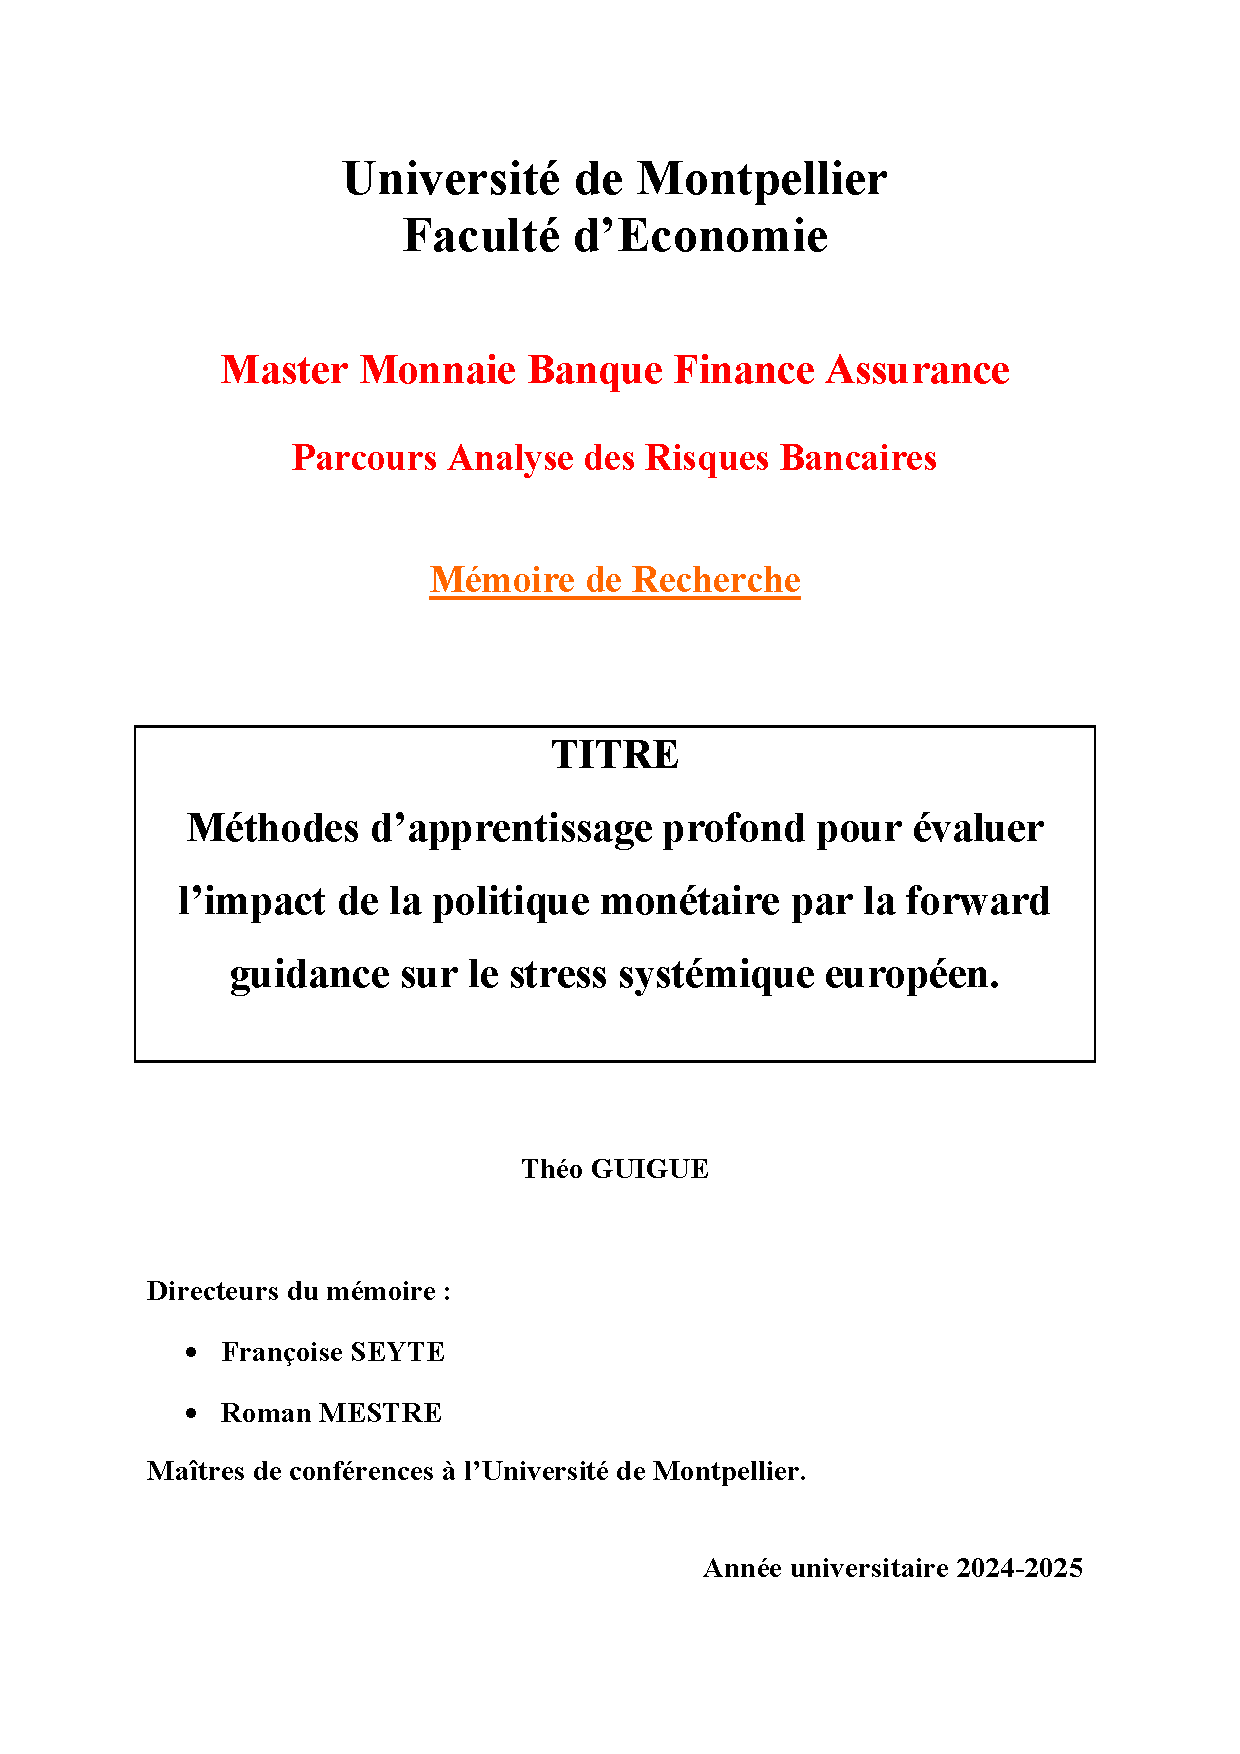
\includepdf[pages=-, pagecommand={}]{page de garde memoire de recherche ARB.pdf}

\newpage

\clearpage
\pagestyle{plain}

\vspace*{0.4\textheight}

\noindent \enquote{\itshape "Le problème central de la prévention des dépressions économiques a été résolu, en pratique, pour de nombreuses décennies."}\bigbreak

\hfill Robert Lucas (prix Nobel d'économie 1995), \textit{Discours présidentiel à l'American Economic Association}, 2003.

\newpage

\phantomsection
\addcontentsline{toc}{chapter}{Remerciements}

\vspace{3em}

\begin{center}
  {\Huge\bfseries Remerciements}
\end{center}

\vspace{1.5em}

\begin{adjustwidth}{2em}{2em}
\begin{sloppypar}

Je tiens à exprimer ma profonde gratitude à Madame \textbf{Françoise Seyte}, pour son accompagnement rigoureux, sa disponibilité constante et la confiance qu’elle m’a accordée tout au long de ce travail en m'y laissant une liberté totale. Sa bienveillance, son exigence méthodologique et la richesse de ses retours ont été déterminantes dans l’élaboration de ce mémoire. Je lui suis infiniment reconnaissant pour l’ensemble de ses conseils, son soutien et l’inspiration qu’elle m’a apportée à chaque étape de cette recherche.\\

Je remercie également Monsieur \textbf{Stéphane Mussard} pour ses conseils éclairés sur les aspects méthodologiques du mémoire, en particulier en ce qui concerne l’apprentissage profond et la modélisation des séries temporelles. Ses suggestions ont grandement enrichi la dimension technique de ce travail, tout en m’incitant à pousser plus loin la rigueur et la précision dans les choix de modélisation.\\

Enfin, je souhaite remercier très chaleureusement Monsieur \textbf{Roman Mestre}, pour son rôle en tant que co-encadrant. Son expertise en macroéconomie monétaire ainsi que ses explications ont contribué à ancrer ce mémoire dans une perspective économique solide et cohérente. Ses conseils ont été précieux pour articuler les enjeux théoriques et empiriques de ce travail.\\

À chacun d’eux, je tiens à témoigner toute ma reconnaissance pour leur accompagnement exigeant, stimulant et toujours bienveillant.
\end{sloppypar}
\end{adjustwidth}

\phantomsection
\addcontentsline{toc}{chapter}{Résumé}

\begin{center}
  {\Huge\bfseries Résumé}
\end{center}

\vspace{1.5em}

\begin{adjustwidth}{2em}{2em}
\begin{sloppypar}
Ce mémoire analyse le rôle de la forward guidance (politique monétaire) de la Banque Centrale Européenne dans la modération ou l’amplification du stress systémique au sein de la zone euro. Dans un contexte post-crise subprimes marqué par des taux d’intérêt à leur borne inférieure suivi d'une normalisation importante post-COVID, la communication anticipative est devenue un instrument central de la politique monétaire. Cependant, son efficacité demeure sujette à débat, notamment lorsque les marchés perçoivent des incohérences entre discours et actions, ou lorsque les chocs macro-financiers rendent les anticipations instables. Afin d’évaluer empiriquement l’impact de la FG sur le stress systémique, ce mémoire adopte une approche pluridisciplinaire mobilisant les outils de traitement automatique du langage et les modèles d’apprentissage profond. À partir d’un corpus de discours officiels de la BCE couvrant la période 2005–2024, plusieurs architectures neuronales sont déployées notamment des Transformers modernes (ModernBERT), modèles séquentiels (Mamba, Mamba-2, Llamba) afin de construire un indicateur sémantique continu de tonalité monétaire. Cet indicateur est ensuite intégré dans des modèles neuroneux temporels (autoencodeurs LSTM et WAE) pour évaluer son pouvoir explicatif sur l’indicateur composite de stress systémique (CISS) développé par la BCE selon différents horizons temporels (court, moyen et long terme). Les résultats mettent en évidence que la FG peut, dans certaines configurations, réduire les tensions sur les marchés financiers, à condition qu’elle soit perçue comme crédible, cohérente et adossée à des mesures concrètes. À l’inverse, une guidance ambiguë ou instable semble perdre de son efficacité, voire amplifier l’incertitude (notamment à long terme). Ce mémoire propose ainsi une lecture renouvelée de la FG comme vecteur de stabilisation systémique, tout en soulignant les limites de son action selon le contexte de normalisation monétaire.
\end{sloppypar}
\end{adjustwidth}

\vspace{2em}

\noindent\textbf{Mots-clés :} \textit{Forward Guidance, Banque Centrale Européenne, Stress Systémique, Deep Learning, Textmining, Politique Monétaire.}



\shorttoc{Sommaire}{0}\addcontentsline{toc}{chapter}{Sommaire}

%------------ Corps du rapport ----------------
\chapter*{Introduction}
\addcontentsline{toc}{chapter}{Introduction}

Depuis les débuts de la politique monétaire moderne, les banques centrales ont cherché à stabiliser l’activité 
économique en régulant les conditions de financement. Durant la majeure partie du XX\textsuperscript{e} siècle, cette 
régulation s’est exercée principalement par l’ajustement des taux d’intérêt directeurs, outil privilégié pour agir sur 
l’inflation, la croissance, ou encore la stabilité externe. Cette logique d’intervention reposait sur un paradigme 
relativement linéaire : en modulant le prix de la monnaie, la banque centrale influençait l’investissement, la 
consommation et, par extension, l’ensemble de l’économie réelle. C’est dans ce cadre que s’est affirmée, à partir des 
années 1990, l’indépendance croissante des banques centrales, accompagnée d’une cible explicite d’inflation, comme 
dans les cas de la Banque d’Angleterre ou de la BCE, créée en 1998 avec pour mandat premier la stabilité des prix 
(Art. 127 TFUE). Cependant, ce cadre d’analyse et d’intervention a été profondément remis en cause par les crises du 
début du XXI\textsuperscript{e} siècle. L’effondrement du système bancaire mondial en 2008, la fragmentation du marché 
obligataire européen durant la crise des dettes souveraines (2010–2012), puis l’épisode de stagnation prolongée 
accompagnée de taux durablement bas, ont mis à l’épreuve la capacité des banques centrales à préserver la stabilité 
financière avec les instruments traditionnels. Lorsque les taux d’intérêt nominaux ont atteint leur borne inférieure 
effective (\textit{zero lower bound}), les leviers classiques ont perdu en efficacité. Dans ce contexte, les autorités monétaires ont été contraintes d’innover.\\

C’est ainsi qu’est apparue, dans les années 2010, une nouvelle catégorie d’outils dits non conventionnels : programmes 
d’achats d’actifs, opérations ciblées de refinancement à long terme, et surtout, Forward Guidance. Cette dernière, 
définie comme une stratégie de communication sur l’orientation future de la politique monétaire, a pour objectif 
d’influencer les anticipations des agents économiques afin de renforcer les effets des mesures prises, même en 
l’absence d’ajustement immédiat des taux. Son efficacité repose sur un mécanisme central de la macroéconomie moderne : 
les décisions économiques présentes dépendent des anticipations futures, lesquelles peuvent être modulées par la 
crédibilité, la clarté et la constance des signaux envoyés par la banque centrale \citep{woodford2012}. 
Parallèlement à cette transformation des instruments monétaires, les préoccupations relatives à la stabilité 
financière se sont accrues. La crise des subprimes a mis en lumière l’existence d’effets de réseau, de phénomènes 
d’illiquidité et de spirales de ventes d’actifs qui, à partir d’un choc initial localisé, peuvent se propager à 
l’ensemble du système économique et menacer sa stabilité. Cette propagation rapide et non linéaire est désignée sous 
le terme de stress systémique. Celui-ci ne se réduit pas à une simple hausse de la volatilité : il exprime une rupture 
de confiance généralisée, une défaillance des canaux de transmission, et une perte de contrôle sur les anticipations 
collectives.\\

La décennie 2010-2020 a été profondément bouleversée par la crise du COVID-19. Face à l’arrêt brutal de l’activité économique et à la hausse généralisée de l’incertitude, la BCE a réactivé massivement sa boîte à outils non conventionnels : achats d’urgence (PEPP), refinancements ultra-accommodants (TLTRO III), et intensification de la forward guidance avec des engagements renforcés sur la trajectoire future des taux et du bilan. La communication de politique monétaire est alors devenue un outil de stabilisation à part entière, jouant un rôle crucial dans la gestion des anticipations des marchés. Mais l’environnement a de nouveau changé à partir de 2022. L’inflation élevée, initialement perçue comme transitoire, s’est enracinée, contraignant la BCE à entamer une phase rapide de resserrement monétaire. Dès lors, un nouveau régime s’installe, marqué par une normalisation des taux d’intérêt, une réduction progressive du bilan, et un repositionnement stratégique de la communication prospective. \citep{hofmann2024ecb} souligne avec justesse que cette transition vers la normalisation a posé des défis inédits pour la forward guidance : les messages prospectifs ont dû s’adapter à une incertitude élevée, à une asymétrie entre les risques de surchauffe et de ralentissement, et à la nécessité de restaurer la crédibilité de la cible d’inflation. Dans cette phase, la FG a évolué d’un instrument d’ancrage à un outil de signalisation conditionnelle, souvent ambiguë, parfois jugée incohérente avec les mesures effectivement prises.

\begin{quote}
\textit{« The ECB’s forward guidance was originally introduced as an instrument to provide additional stimulus when policy rates were close to their lower bound. However, in the post-pandemic context, forward guidance may have lost part of its effectiveness due to shifting macroeconomic risks, market scepticism, and policy reversals. »}
\hfill \citep{hofmann2024ecb}
\end{quote}

Cette séquence souligne un point important qu'il est nécessaire de bien comprendre dans l'environnement macro-monétaire : la FG est devenue un élément structurant de la politique monétaire contemporaine, mais dont les effets ne sont ni constants ni univoques. Son efficacité dépend du régime macro-financier dans lequel elle s’insère, des anticipations qu’elle façonne, et des réactions de marché qu’elle suscite. Dans un monde de plus en plus interconnecté, où les marchés sont instantanément réactifs aux signaux politiques, monétaires et géopolitiques, la surveillance du stress systémique est devenue une priorité pour les régulateurs.\\

Au-delà à ces transformations économiques et institutionnelles, une révolution technologique silencieuse a profondément modifié les méthodes d’analyse des textes économiques : l’émergence de l’intelligence artificielle, et en particulier du deep learning. Ce recours aux méthodes de deep learning n’est pas simplement motivé par un effet de mode technologique, mais par des considérations théoriques et empiriques. Les discours de politique monétaire, en particulier ceux de la BCE, présentent des caractéristiques linguistiques complexes : redondance stratégique, prudence lexicale, multiplicité des registres, présence de signaux implicites. Ces éléments rendent les méthodes économétriques classiques peu adaptées à leur analyse fine, notamment lorsqu’il s’agit d’identifier des tonalités latentes ou d’extraire des signaux prospectifs non linéaires. De plus, la dynamique du stress systémique est elle-même marquée par des non-linéarités et des régimes multiples qui nécessitent des modèles capables d’apprendre des structures complexes à partir des données. Les architectures neuronales modernes, en particulier les Transformers et les autoencodeurs variationnels régularisés, offrent précisément cette capacité d’apprentissage profond, en s’affranchissant des hypothèses paramétriques trop restrictives. Leur utilisation dans ce mémoire répond donc à un double besoin : celui de capter la richesse sémantique des textes économiques, et celui de modéliser les dynamiques complexes du stress financier de manière flexible et performante.\\

Longtemps réservées aux sciences du langage ou de l’image, les techniques d’apprentissage profond ont progressivement conquis la recherche en économie, en finance, et plus récemment en macroéconomie monétaire. Leur capacité à extraire des régularités complexes dans des données non structurées a ouvert de nouvelles perspectives pour l’analyse des discours des banques centrales, des procès-verbaux de réunion, ou encore des communiqués de presse de politique monétaire. Les premières applications ont reposé sur des modèles de classification supervisée ou sur des représentations vectorielles simples comme TF-IDF. Mais depuis la fin des années 2010, ce champ a été bouleversé par l’apparition d’architectures neuronales de type Transformers \citep{vaswani2017attention}, dont les performances dépassent celles des modèles récurrents traditionnels. Leurs mécanismes d’attention permettent de capturer efficacement les dépendances contextuelles dans des séquences textuelles longues, ce qui est particulièrement adapté au traitement des discours économiques, riches en subtilités sémantiques, en métaphores prudentes et en signaux implicites. Ces modèles ont été rapidement adoptés dans les banques centrales elles-mêmes : la BCE, la Fed ou encore la Banque d’Angleterre ont multiplié les travaux internes mobilisant BERT, GPT ou leurs déclinaisons pour évaluer la tonalité des discours, mesurer l’incertitude linguistique ou anticiper les réactions de marché \citep{gali2008,hansen2016}. Plus récemment, de nouvelles variantes de Transformers à mémoire longue ou à structure d’état comme Mamba ou Llamba ont émergé, permettant de mieux modéliser les dépendances temporelles dans des séries de textes économiques publiés à intervalles réguliers. Couplés à des architectures probabilistes comme les autoencodeurs variationnels ou les Wasserstein Auto-Encoders (WAE), ces outils autorisent une modélisation fine et continue de la tonalité monétaire. Cette convergence entre techniques de traitement automatique du langage, apprentissage profond et économétrie appliquée constitue aujourd’hui un champ de recherche en plein essor, dans lequel ce mémoire se propose en prolongation.\\

Donc dans un monde de plus en plus interconnecté, où les marchés sont instantanément réactifs aux signaux politiques, 
monétaires et géopolitiques, la surveillance du stress systémique est devenue une priorité pour les régulateurs avec de nouvelles méthodes qui permettent d'extraire ces signaux. Les 
banques centrales ne peuvent plus se limiter à l’atteinte d’une cible d’inflation ou à la régulation des agrégats 
monétaires. Elles doivent aussi veiller à la stabilité globale du système financier, coordonner leurs actions avec les 
autorités macroprudentielles, et intégrer dans leurs décisions les risques de contagion entre marchés. L’indicateur  composite de stress systémique (CISS), développé par la BCE \citep{hollo2012ciss}, incarne cette volonté de 
quantifier et de surveiller les tensions financières multidimensionnelles dans une logique systémique. Alors, les 
instruments monétaires s’étendent au-delà des ajustements techniques pour devenir des outils de communication 
stratégique. \textbf{L'objectif de ce mémoire est donc d'étudier l'impact de la Forward Guidance de la Banque Centrale Européenne sur le stress systémique, en particulier sa capacité à stabiliser le système économique ou amplifier les tensions en période de crise}. En d’autres termes, la  communication de la banque centrale est-elle en mesure de stabiliser les anticipations collectives et d’éviter les 
comportements mimétiques qui fragilisent le système ? Ou bien, au contraire, peut-elle devenir un facteur 
d’instabilité lorsqu’elle est perçue comme ambiguë, réversible ou incohérente avec les actions prises ? Cette 
interrogation conduit à une problématique plus générale :

\begin{quote}
\textit{Dans quelle mesure la communication anticipative de la politique monétaire européenne (en particulier à travers la forward guidance) permet-elle de réduire l’incertitude des marchés financiers et de prévenir les dynamiques de contagion systémique ? Ou, au contraire, peut-elle, lorsqu’elle est perçue comme ambiguë ou non crédible, amplifier les tensions sur les marchés interconnectés pour se propager à l'ensemble du système ?}
\end{quote}

Répondre à cette problématique suppose de quantifier le contenu sémantique des discours de la BCE, de modéliser leur impact temporel sur des indicateurs agrégés de stress, et d’identifier les conditions (forme, période, tonalité) sous lesquelles la forward guidance agit comme facteur stabilisateur ou déstabilisant. Cela nécessite l’articulation d’une approche théorique, computationnelle et empirique, que ce mémoire s’attache à développer.\\

Ainsi, ce mémoire se propose d’examiner la forward guidance non plus uniquement comme un outil de stabilisation conjoncturelle, mais comme un vecteur potentiel de réduction ou d’amplification du stress systémique au sein de la zone euro. L’hypothèse sous-jacente est que la nature, la fréquence et la cohérence des communications officielles de la BCE peuvent conditionner l’intensité des tensions sur les marchés financiers. Une guidance crédible, perçue comme cohérente et assortie d’engagements opérationnels tangibles, pourrait apaiser les anticipations et réduire les comportements de panique. À l’inverse, une guidance floue ou sujette à révision pourrait accroître l’incertitude et catalyser des dynamiques de contagion financière. Cette réflexion est d’autant plus pertinente dans le cadre européen, où l’unicité de la politique monétaire cohabite avec une diversité institutionnelle, économique et budgétaire propre à engendrer des divergences de perception et des fragilités structurelles. Ce travail de recherche entend donc apporter une contribution originale à la littérature économique et financière, en associant trois dimensions complémentaires. Pour commencer, une lecture historique et analytique de l’évolution de la politique monétaire de la BCE, et de la place grandissante qu’y occupe la forward guidance depuis la crise financière de 2008. Ensuite, une approche textuelle et computationnelle innovante, fondée sur les outils du traitement automatique du langage et de l’apprentissage profond, pour extraire un indicateur sémantique de forward guidance à partir des discours de la BCE. Enfin, une évaluation empirique de l’impact de cet indicateur sur le stress systémique, à travers des modèles neuronaux, avec une attention particulière portée à la robustesse des résultats et aux implications de politique économique. Pour ce faire, le mémoire est structuré en trois chapitres, chacun répondant à une étape clé de la problématique.\\

Le premier chapitre traite donc des fondations théoriques de l’analyse économique. Il débute par une rétrospective de la politique monétaire européenne, depuis la mise en place des taux directeurs par la BCE à la fin des années 1990, jusqu’aux évolutions récentes en contexte post-pandémique. Les instruments traditionnels sont confrontés aux limites de la borne zéro, ce qui ouvre la voie à des outils non conventionnels. La forward guidance est ensuite étudiée dans sa diversité : qualitative, basée sur des délais ou conditionnelle à des indicateurs économiques. Ses mécanismes de transmission sont détaillés à travers le prisme des taux d’intérêt futurs, des anticipations d’inflation, des conditions de financement et des signaux macroéconomiques. Enfin, le chapitre introduit la notion de stress systémique, sa conceptualisation théorique, ses canaux de propagation (effets domino, interdépendances de marché, spirales d’illiquidité), et ses instruments de mesure. L’indicateur composite de stress systémique (CISS) y tient une place centrale, car il permet de quantifier les tensions agrégées dans un cadre temporel et sectoriel.
Le deuxième chapitre est consacré à l’outillage méthodologique mobilisé pour répondre à l’objectif de recherche. Il présente les fondements des réseaux neuronaux appliqués au langage naturel, depuis les word embeddings jusqu’aux Transformers, avec un accent mis sur les variantes modernes utilisées dans ce mémoire (ModernBERT, Mamba, Mamba-2 et Llamba). Ces architectures permettent d’extraire une représentation vectorielle contextualisée des textes, propre à capter la tonalité, les nuances sémantiques et la structure logique des discours de politique monétaire. Le chapitre expose ensuite les principes des autoencodeurs variationnels et en particulier des Wasserstein Auto-Encoders (WAE), utilisés pour la régularisation de l’espace latent textuel et temporel. L’ensemble de ces techniques est mobilisé pour construire un indicateur continu de forward guidance, permettant de quantifier la tonalité monétaire (expansionniste, neutre, restrictive) des discours officiels de la BCE sur une période allant de 2005 à 2024.
Le troisième chapitre met en œuvre l’application empirique. À partir d’un corpus structuré des publications officielles de la BCE (communiqués de politique monétaire, discours présidentiels, conférences de presse), un indicateur de forward guidance est généré pour chaque date de décision. Ce score est ensuite intégré dans différents modèles prédictifs du stress systémique : régressions Ridge pénalisées pour éviter le sur-ajustement, modèles à mémoire courte (LSTM) et modèles à espace d’état (Mamba) pour la dynamique temporelle. Une attention particulière est portée à la comparaison entre modèles, aux horizons temporels d’impact (court, moyen, long terme) et à la robustesse des résultats. L’analyse empirique permet d’identifier les configurations dans lesquelles la FG contribue effectivement à réduire les tensions de marché, et celles où elle perd en efficacité, voire génère de l’instabilité. 
Enfin, ce dernier chapitre s’ouvre sur une discussion normative, qui plaide pour une intégration renforcée entre forward guidance et instruments de régulation macroprudentielle. Il est notamment suggéré que la communication monétaire gagne à être systématiquement adossée à des mesures concrètes, telles que la publication de calendriers d’intervention, l’activation de T-LTRO, ou la coordination avec les politiques de coussins contracycliques. Cette approche intégrée permettrait d’accroître la crédibilité de la guidance et de renforcer son effet de signal en période de tensions financières.\\

En définitive, ce mémoire ambitionne de mettre en lumière la puissance mais aussi les fragilités d’un outil devenu central dans les dispositifs de politique monétaire contemporaine.



\chapter{Politique monétaire, forward guidance et stress systémique dans le cadre européen}
\mtcaddchapter
\minitoc

Dans un monde de plus en plus interconnecté où les crises se succèdent et ne se ressemblent pas, la stabilité économique et financière est l'enjeu le plus important pour assurer le bon fonctionnement du système global. Dans le cadre européen, cette stabilité repose en grande partie sur les actions de la BCE. Depuis sa création, la BCE a pour mission principale de garantir la stabilité des prix, un objectif central inscrit dans les traités européens. Cependant, la politique monétaire menée par la BCE a considérablement évolué au fil du temps, en réponse aux transformations économiques et aux crises successives qui ont mis sous pression le système financier européen. Historiquement, la politique monétaire reposait essentiellement sur des instruments conventionnels, tels que l’ajustement des taux directeurs et le contrôle de la liquidité bancaire à travers des opérations de refinancement. Toutefois, les chocs financiers majeurs de ces dernières décennies (notamment celle de 2008, des dettes souveraines en zone euro, plus récemment le COVID) ont profondément modifié le cadre d’action des banques centrales. Face à des situations inédites de taux d’intérêt proches de zéro et à des risques accrus d’instabilité financière, la BCE a dû innover et adopter de nouveaux outils pour assurer une transmission efficace de la politique monétaire. Parmi ces évolutions, la forward guidance s’est imposée comme un instrument central. Cette approche, qui consiste à fournir des indications sur l’orientation future de la politique monétaire, vise à influencer les anticipations des marchés et à renforcer l’impact des décisions monétaires sur l’économie réelle. En période de taux d’intérêt bas prolongés, où la marge de manœuvre des banques centrales se réduit, la forward guidance joue un rôle essentiel en stabilisant les anticipations et en facilitant la transmission de la politique monétaire. Cependant, son efficacité repose largement sur la crédibilité de la banque centrale et sur la cohérence des signaux envoyés aux investisseurs.

Parallèlement à ces évolutions monétaires, le stress systémique est devenu une préoccupation importante des décideurs économiques et des institutions financières. Le stress systémique désigne des tensions financières de grande ampleur qui, lorsqu’elles émergent, peuvent compromettre la stabilité du système financier dans son ensemble, il est signifié de réaction en chaîne ou d'effet domino. Ces tensions peuvent résulter de chocs exogènes, comme une crise bancaire, une forte volatilité des marchés ou encore une dégradation soudaine des conditions de financement. Si ces tensions ne sont pas contenues à temps, elles peuvent se propager rapidement via des effets de contagion et entraîner des répercussions négatives sur l’ensemble de l’économie. Les crises financières récentes ont illustré la vulnérabilité des marchés face à ces épisodes de stress prolongé. La crise des subprimes en 2008, qui a déclenché un effondrement mondial du système financier, et la crise des dettes souveraines en zone euro, qui a exacerbé les divergences entre les économies européennes, ont montré à quel point l’interconnexion des marchés pouvait amplifier la transmission des chocs. Ces événements ont poussé la BCE et d’autres institutions de régulation à renforcer leur surveillance des risques systémiques et à développer des outils de mesure plus sophistiqués. L’un des instruments clés dans ce domaine est l’Indicateur Composite de Stress Systémique (CISS), conçu pour évaluer les tensions financières en agrégeant plusieurs dimensions du stress de marché. Cet indicateur permet d’anticiper les périodes de vulnérabilité et de guider les actions des autorités monétaires afin de limiter les risques de contagion. Dans ce contexte, l’interaction entre politique monétaire, forward guidance et stress systémique constitue un sujet de recherche essentiel pour mieux comprendre comment la communication stratégique des banques centrales peut influencer la stabilité financière. Alors que la forward guidance est censée réduire l’incertitude et stabiliser les marchés en fournissant une trajectoire claire pour les taux d’intérêt, son impact sur le stress systémique reste une question ouverte. Dans certaines situations, une forward guidance mal calibrée ou perçue comme peu crédible peut au contraire accentuer la volatilité des marchés et amplifier les tensions financières.\\

L’objectif de ce chapitre est donc mettre en exergue et d’analyser comment la politique monétaire et la forward guidance interagissent avec le stress systémique en zone euro. Cette réflexion se structurera autour de trois grands axes. Les fondements de la politique monétaire en zone euro seront tout d’abord examinés. Cette section reviendra sur les objectifs et les instruments de la BCE, en mettant en lumière les transformations qu’a connues la politique monétaire européenne face aux crises successives. L’évolution des outils monétaires, de l’ère des instruments conventionnels aux politiques non conventionnelles, sera détaillée afin d’offrir une vision claire du cadre d’action actuel de la BCE. La forward guidance sera ensuite analysée comme un instrument clé de la politique monétaire moderne. Après une présentation de ses différentes formes cette section étudie les mécanismes par lesquels la forward guidance influence les anticipations et les marchés financiers. Les défis liés à sa mise en œuvre, notamment en matière de crédibilité et de cohérence des signaux monétaires, seront également abordés. La problématique du stress systémique et son interaction avec la forward guidance seront enfin approfondies. Cette dernière section mettra en évidence le rôle du CISS dans l’évaluation du stress financier et examinera comment la communication des banques centrales peut atténuer ou, au contraire, amplifier les tensions sur les marchés. L’importance de la coordination entre politique monétaire et régulation macroprudentielle sera également discutée, afin de comprendre comment ces deux leviers peuvent être articulés pour mieux gérer le risque systémique.

\section{Fondements de la politique monétaire}

Depuis sa création en 1998, la BCE a adopté une stratégie monétaire fondée sur une approche analytique et l’utilisation d’instruments adaptés aux évolutions du contexte économique et financier. Alors, l’objectif de cette section est d’analyser les fondements de la politique monétaire en zone euro, en mettant en évidence ses objectifs, ses stratégies et ses instruments. Cette analyse se déploie en trois temps. Tout d'abord, par une définition et objectifs de la politique monétaire avec une présentation des principes fondamentaux qui guident la politique monétaire en mettant l’accent sur le mandat de la BCE, son cadre institutionnel et les objectifs qu’elle poursuit. Aussi, il sera également présenté comment ces objectifs ont évolué dans le temps, notamment en réponse aux crises financières. Ensuite, il sera abordé les piliers de la stratégie monétaire de la BCE. Dans ce cadre, il sera mis en évidence l'analyse adopté par la BCE, en détaillant l’approche des deux piliers (analyse économique et monétaire) qui guide ses décisions. Cette section mettra en exergue les fondements théoriques et empiriques de cette stratégie, ainsi que les critiques qui lui sont adressées. Pour finir, l'évolution des instruments de la politique monétaire sera présenté historiquement ; l’ère de la stabilité initiale (1999-2008), marquée par l’utilisation d’outils conventionnels. La crise financière et la transformation de la politique monétaire (2008-2015), qui a vu l’introduction de mesures non conventionnelles comme les opérations de refinancement à long terme et les programmes d’achats d’actifs. La période post-crise et les défis de l’inflation basse (2015-2021), avec un recours accru à la forward guidance et aux politiques d’assouplissement quantitatif. La phase de normalisation et le choc inflationniste (2022-2024), qui marque un retour progressif à une politique plus restrictive face à une inflation élevée. Cela permettra de comprendre comment la BCE a dû adapter sa stratégie et ses outils en réponse aux défis économiques et financiers comtemporains, et comment la politique monétaire en zone euro est devenue un élément structurant de la stabilité macroéconomique et financière. Cette exploration permettra également de mieux comprendre l’importance croissante de la communication et des interactions entre la politique monétaire et les marchés financiers dans un contexte de plus en plus complexe et incertain.

\subsection{Définition et objectifs de la politique monétaire}

La politique monétaire repose sur un cadre d’analyse structuré permettant d’anticiper et de gérer les fluctuations économiques. Dans le cas de la BCE, cette approche s’articule autour de deux piliers complémentaires, combinant une évaluation des dynamiques économiques à court et moyen terme et une surveillance des évolutions monétaires susceptibles d’influencer l’inflation. Ces deux dimensions permettent d’assurer une prise de décision fondée sur une vision globale des risques pesant sur la stabilité des prix et l’activité économique.

\subsubsection{Définition}

La politique monétaire désigne l’ensemble des actions entreprises par une banque centrale pour réguler l’offre de monnaie et influencer les conditions financières dans une économie. Son objectif principal est d’assurer la stabilité des prix, c’est-à-dire maintenir l’inflation à un niveau compatible avec une croissance économique stable. La  BCE, en tant qu’autorité monétaire de la zone euro, a inscrit cet objectif dans son mandat, conformément à l’article 127 du Traité sur le Fonctionnement de l’Union Européenne (TFUE). La cible d’inflation est définie comme proche mais inférieure à 2\% à moyen terme (BCE, 2021).\\

Outre la stabilité des prix, la politique monétaire poursuit d’autres objectifs secondaires, notamment le soutien à la croissance économique et à l’emploi, conformément à l’approche flexible adoptée par la BCE depuis la crise financière de 2008 (Draghi, 2014). La stabilité financière, bien que non explicitement inscrite dans le mandat initial, est devenue une préoccupation majeure, comme en témoignent les mesures non conventionnelles mises en place après la crise des dettes souveraines en zone euro \citep{smets2003}.

\subsubsection{Les deux pilliers}

Depuis sa création en 1998, la BCE a adopté une stratégie monétaire fondée sur l’approche des "deux piliers", introduite par \citep{issing2001}. Cette approche permet d’évaluer les risques pesant sur la stabilité des prix en combinant une analyse économique et une analyse monétaire.\\

Le premier pilier, basé sur l’analyse économique, vise à évaluer les évolutions conjoncturelles susceptibles d’influencer l’inflation à court et moyen terme. Il repose sur l’examen de plusieurs indicateurs macroéconomiques, notamment la croissance du PIB, qui permet d’anticiper la dynamique économique globale, et le taux de chômage, qui donne des indications sur les pressions inflationnistes via le marché du travail \citep{blanchard1986}. Par ailleurs, l’évolution des prix des matières premières et des chocs d’offre externes est analysée pour détecter d’éventuels facteurs exogènes affectant l’inflation. Enfin, les conditions de financement, incluant les taux d’intérêt et l’accès au crédit bancaire, sont prises en compte pour évaluer la transmission de la politique monétaire et son effet sur l’activité économique \citep{smets2003}.\\

Le deuxième pilier, fondé sur l’analyse monétaire, repose sur l’idée que l’évolution de la masse monétaire joue un rôle clé dans la dynamique de l’inflation à long terme, en accord avec les théories monétaristes \citep{friedman1968}. Ainsi, la BCE surveille la croissance des agrégats monétaires, notamment M3, qui mesure la quantité de monnaie en circulation et son impact potentiel sur l’inflation. L’évolution du crédit bancaire est également étudiée, car elle reflète la transmission de la politique monétaire et son influence sur la consommation et l’investissement. En complément, la BCE analyse le comportement des institutions financières et les dynamiques des taux d’intérêt pour détecter d’éventuelles tensions financières susceptibles d’affecter l’économie réelle. Toutefois, certains économistes, comme \citep{gali2008}, ont critiqué la pertinence du second pilier, estimant que la relation entre masse monétaire et inflation est devenue plus floue dans un environnement de taux bas.\\

En réaction à des pilliers, une manière courante de modéliser la réaction de la politique monétaire aux variations macroéconomiques est la règle de Taylor, qui définit le taux d'intérêt nominal $i_t$ en fonction de l'inflation et de l'écart de production mais aussi de ses valeurs passées :

\begin{equation}
i_t = r^* + \pi_t + \sum_{k=0}^{K} \alpha_k (\pi_{t-k} - \pi^*) + \sum_{j=0}^{J} \beta_j (y_{t-j} - y^*)
\end{equation}

où  \( i_t \) est le taux directeur de la BCE à l’instant \( t \), \( r^* \) est le taux d’intérêt naturel, \( \pi_t \) est le taux d’inflation observé, \( \pi^* \) est la cible d’inflation de la BCE (proche mais inférieure à 2\%), \( y_t \) est le PIB réel, \( y^* \) est le PIB potentiel, \( \alpha \) et \( \beta \) sont les paramètres de réaction de la BCE à l’inflation et à l'écart de production. Cette équation traduit la manière dont la BCE ajuste ses taux en fonction de l’inflation et de l’écart de production. Une hausse de l’inflation au-delà de la cible ou une surchauffe économique incite la BCE à relever ses taux, tandis qu’une faible inflation ou un ralentissement économique justifie une politique monétaire plus accommodante.\\

Pour assurer la réalisation de ses objectifs, la politique monétaire s’appuie sur un ensemble d’instruments dont la nature et l’utilisation ont évolué au fil du temps. Si les outils traditionnels fondés sur la gestion des taux d’intérêt ont longtemps constitué la principale action des banques centrales, les bouleversements économiques et financiers des deux dernières décennies ont conduit à un élargissement et à une redéfinition de ces instruments.

\subsection{Évolution des instruments de la politique monétaire européenne}

L’évolution de la politique monétaire européenne reflète les transformations majeures qu’a connues la BCE face aux crises et aux mutations économiques. D’abord, la période de stabilité initiale (1999-2008) est abordée, illustrant une gestion classique des taux d’intérêt et de la liquidité bancaire. Ensuite, l’impact de la crise financière de 2008 et l’introduction d’instruments non conventionnels sont examinés, marquant une rupture avec les pratiques antérieures. La période post-crise et la problématique de l’inflation basse (2015-2021) sont ensuite analysées, soulignant l’importance croissante du quantitative easing et de la forward guidance. Enfin, la normalisation monétaire entamée à partir de 2022 face au choc inflationniste est présentée, mettant en lumière les défis actuels de la BCE dans un environnement économique incertain.\\

\subsubsection{L'ère de la stabilité initiale (1999-2008)}

Lors de sa création en 1999, la BCE a adopté une approche conventionnelle de la politique monétaire, inspirée des principes établis par la Bundesbank allemande. Durant cette période, l’outil principal de la BCE reposait sur la gestion des taux directeurs, notamment le taux de refinancement principal, utilisé pour contrôler l’inflation et stabiliser la croissance économique.\\

Durant cette décennie, la politique monétaire de la BCE était relativement prévisible et suivait une logique cyclique : les taux d’intérêt étaient ajustés en fonction de l’évolution de l’inflation et de la croissance. Par exemple, après la récession de 2001-2002 consécutive à l’éclatement de la bulle technologique, la BCE a progressivement réduit ses taux pour soutenir l’activité économique, avant de les relever à partir de 2005 pour contrer les tensions inflationnistes \citep{angeloni2003}. L’ensemble des opérations de refinancement (MRO, LTRO) était également utilisé dans une logique d’ajustement régulier de la liquidité bancaire, sans nécessiter d’intervention massive.

\newpage

Cependant, malgré cette stabilité apparente, des fragilités structurelles se sont développées, notamment une forte expansion du crédit et une augmentation de la prise de risque sur les marchés financiers, accentuées par une intégration croissante des économies européennes au sein de la zone euro \citep{bernanke2001}. Ces déséquilibres allaient se matérialiser de manière brutale avec la crise financière de 2008, marquant la fin de cette période de relative sérénité monétaire.

\subsubsection{La crise financière et la transformation de la politique monétaire (2008-2015)}

L’effondrement de Lehman Brothers en septembre 2008 marque un tournant important pour la politique monétaire mondiale et oblige la BCE à revoir en profondeur ses instruments d’intervention \citep{reinhart2009}. Face à un effondrement du crédit interbancaire, la BCE réduit drastiquement son taux de refinancement, passant de 4,25\% en juillet 2008 à 1\% en mai 2009 (ECB, 2009). Cependant, la persistance des tensions financières et la fragmentation du marché obligent l’institution à adopter des instruments non conventionnels, marquant une rupture avec son cadre initial et les traités européens signés à l'origine.\\

La BCE introduit ainsi les opérations de refinancement à long terme (LTROs), accordant des prêts massifs aux banques pour stabiliser le système financier \citep{coeuré2013}. Ces mesures visent à restaurer la transmission de la politique monétaire en assurant aux banques une liquidité suffisante pour financer l’économie réelle. Cependant, la crise des dettes souveraines de la zone euro (2010-2012) expose les limites des outils traditionnels : les écarts de taux entre les obligations d’État des différents pays de la zone euro s’élargissent dangereusement, menaçant l’intégrité même de l’union monétaire \citep{degrauwe2012}.\\

Face à cette crise existentielle, la BCE innove avec l’annonce du programme "Outright Monetary Transactions" (OMT) en 2012, qui permet d’acheter des obligations souveraines sous conditions. Mais c’est surtout le discours de Mario Draghi en juillet 2012, affirmant que la BCE fera "tout ce qu’il faudra" pour préserver l’euro, qui marque un tournant décisif (Draghi, 2012). Cette déclaration stabilise les marchés, illustrant l’importance croissante de la communication stratégique comme instrument de politique monétaire.

\subsubsection{La période post-crise et le défi de l’inflation basse (2015-2021)}

Après la crise des dettes souveraines, la zone euro entre dans une phase prolongée de faible inflation, voire de risque de déflation. La reprise économique reste fragile, et les anticipations d’inflation sont mal ancrées \citep{blanchard2015}. Confrontée à cette situation, la BCE adopte un arsenal monétaire encore plus expansif, mettant en place des mesures inédites dans l’histoire de la politique monétaire européenne.\\

L’instrument clé de cette période est le programme d’achats d’actifs (Quantitative Easing, QE) lancé en mars 2015 sous le nom de Public Sector Purchase Programme (PSPP). Ce programme consiste à acheter massivement des obligations souveraines et privées afin de faire baisser les taux d’intérêt à long terme et stimuler l’investissement et la consommation \citep{gürkaynak2015}. En complément, la BCE approfondit sa forward guidance, en s’engageant à maintenir des taux bas "aussi longtemps que nécessaire" pour ancrer les anticipations inflationnistes \citep{woodford2012}.\\

Une autre innovation majeure est l’introduction des opérations ciblées de refinancement à long terme (TLTROs), qui incitent les banques à accorder plus de crédits aux entreprises et ménages en leur offrant des conditions avantageuses \citep{altavilla2019}. Malgré ces efforts, l’inflation reste structurellement inférieure à l’objectif, en raison de facteurs démographiques, technologiques et de faiblesse de la demande \citep{blanchard2019}.\\

Le choc de la pandémie de Covid-19 en 2020 pousse la BCE à aller encore plus loin avec le Programme d’Achat d’Urgence face à la Pandémie (PEPP), un QE flexible visant à éviter une fragmentation financière excessive et à stabiliser l’économie. Ces actions marquent l’apogée des instruments non conventionnels, avec une politique monétaire extrêmement accommodante pour soutenir la reprise.

\subsubsection{Le choc inflationniste et la normalisation de la politique monétaire (2022-2024)}

Après une décennie de politique ultra-accommodante, le contexte change brutalement en 2022 avec un choc inflationniste majeur. La sortie de la pandémie, les perturbations des chaînes d’approvisionnement et la flambée des prix de l’énergie, exacerbée par la guerre en Ukraine, propulsent l’inflation bien au-delà de l’objectif de 2\%, atteignant 10,6\% en octobre 2022 (ECB, 2022).\\

Face à cette situation, la BCE amorce une normalisation rapide de sa politique monétaire sous la présidence de Christine Lagarde. En juillet 2022, elle met fin à son programme d’achats d’actifs, puis engage une série de hausses des taux directeurs, la première en plus de 10 ans. Le taux de refinancement, qui était à 0\% depuis 2016, est progressivement remonté pour atteindre 4,5\% en 2023 (ECB, 2023).\\

Cette phase de resserrement monétaire vise à freiner la demande et contenir l’inflation, au prix d’un ralentissement économique. Cependant, la BCE doit gérer un équilibre délicat entre lutte contre l’inflation et risque de récession, tout en évitant une fragmentation excessive des marchés obligataires de la zone euro. Pour y parvenir, elle introduit en 2022 le Transmission Protection Instrument (TPI), destiné à limiter les écarts de taux entre les États membres \citep{lane2023}.\\

En 2024, bien que l’inflation ait commencé à ralentir, les incertitudes restent fortes, et la BCE doit ajuster son action en fonction des perspectives économiques et financières. Cette période illustre le retour à une politique monétaire plus classique, mais avec un cadre profondément transformé par l’expérience des crises précédentes et l’usage d’instruments non conventionnels.\\

Parallèlement à ces ajustements, le rôle de la forward guidance et de la communication monétaire devient de plus en plus central. La BCE doit désormais convaincre les marchés que son action est efficace sans créer d’effets secondaires indésirables. L’incertitude économique oblige la banque centrale à ajuster ses discours et ses projections pour éviter des mouvements de panique ou d’anticipations excessives d’une récession \citep{nakamura2018}. Cette évolution illustre une tendance structurelle : la politique monétaire ne repose plus uniquement sur des décisions techniques, mais aussi sur la manière dont ces décisions sont perçues et anticipées par les acteurs économiques.\\

Ainsi, l’évolution de la politique monétaire européenne reflète les défis successifs auxquels la BCE a dû faire face, passant d’une gestion traditionnelle des taux d’intérêt à l’utilisation d’instruments non conventionnels en réponse aux crises financières et à la faiblesse persistante de l’inflation. Ainsi, il est essentiel de comprendre avant tout comment la politique monétaire se diffuse à travers les marchés.

\subsection{Transmission de la politique monétaire et interactions avec les marchés}

Avant d’examiner le rôle spécifique de la forward guidance dans le dispositif de transmission de la politique monétaire, il convient de revenir sur les fondements généraux de cette transmission. Celle-ci repose sur un ensemble de canaux identifiés dans la littérature, par lesquels les décisions de la banque centrale influencent l’économie réelle. Ces canaux, à la fois théoriques et empiriques, permettent d’évaluer l'efficacité des instruments monétaires selon les contextes macro-financiers.

\subsubsection{Les canaux de transmission de la politique monétaire : fondements théoriques et empiriques}

La transmission de la politique monétaire à l'économie réelle s'effectue à travers plusieurs canaux identifiés dans la littérature économique : le canal des taux d'intérêt, le canal du crédit bancaire, le canal du taux de change, et le canal des anticipations. Ces canaux sont largement étudiés dans les travaux de \citep{bernanke1995}, \citep{mishkin1996}, \citep{mishkin2001} et plus récemment par \citep{gertler2015} et \citep{boivin2010}. Ces mécanismes permettent d'évaluer l'efficacité des politiques monétaires menées par les banques centrales.\\

Le canal des taux d'intérêt repose sur l'idée que la politique monétaire influence directement les taux de marché à court terme, modifiant ainsi le coût du capital pour les entreprises et les ménages. Selon \citep{clarida2000}, les ajustements de taux directeurs sont censés influencer les décisions d'investissement et de consommation. Cependant, comme le souligne \citep{adrian2010}, en période de stress financier, la transmission peut être entravée par une augmentation des primes de risque.\\

Le canal du crédit bancaire souligne l’importance des institutions financières comme intermédiaires indispensables. Selon \citep{kashyap2000}, la contraction monétaire réduit la disponibilité du crédit en augmentant les contraintes de financement des banques, entraînant une diminution des prêts aux agents économiques. Ce phénomène est particulièrement exacerbé en période de crise financière, comme l'ont démontré \citep{ivashina2010} lors de la crise de 2008.

Le canal du taux de change est particulièrement pertinent dans les économies ouvertes. \citep{obstfeld2005} mettent en évidence que les variations des taux d'intérêt directeurs influencent fortement le taux de change et par conséquent les flux commerciaux et financiers. \citep{rey2015} montre que dans un contexte de forte mobilité internationale des capitaux, les marchés financiers internationaux amplifient ces effets, conduisant à une synchronisation accrue des cycles économiques à travers les pays.

Le canal des anticipations est fondé sur le concept de forward guidance, étudié notamment par \citep{woodford2012} et \citep{delnegro2015}. Ce canal met l'accent sur la capacité des banques centrales à influencer les anticipations des agents économiques à travers une communication crédible et transparente concernant l'orientation future des politiques monétaires.

\subsubsection{Interactions avec les marchés financiers : implications pour la politique monétaire}

Les marchés financiers jouent un rôle clé dans l'amplification ou l'atténuation des effets des politiques monétaires. Une littérature croissante, dont \citep{brunnermeier2014} et \citep{adrian2014}, souligne comment les conditions financières peuvent influencer la transmission monétaire en périodes normales comme en périodes de crise.

En période de tensions financières, comme observés durant la crise financière globale, les marchés deviennent particulièrement sensibles aux signaux des banques centrales, exacerbant les effets des annonces de politique monétaire. \citep{brunnermeier2009} montrent notamment comment les contraintes de liquidité sur les marchés financiers peuvent aggraver la transmission des chocs monétaires négatifs à l'économie réelle.

Par ailleurs, les travaux de \citep{gilchrist2012} et \citep{caldara2019} mettent en évidence l'importance des primes de risque financières comme indicateur clé influençant la transmission monétaire. En effet, des augmentations significatives des primes de risque peuvent neutraliser partiellement l'effet expansionniste d'une baisse des taux directeurs, notamment lorsque les marchés financiers anticipent une augmentation du risque de défaut.

Enfin, la communication et la crédibilité des banques centrales constituent des dimensions fondamentales pour gérer les interactions avec les marchés financiers. Selon \citep{hansen2016}, une communication claire réduit l'incertitude sur les marchés financiers et améliore ainsi la transmission monétaire. Inversement, une communication ambigüe peut aggraver la volatilité des marchés et compliquer l'atteinte des objectifs de politique monétaire.\\

L’analyse des fondements de la politique monétaire en zone euro a mis en évidence la transformation progressive du cadre d’intervention de la BCE face aux évolutions économiques et financières. Initialement fondée sur une gestion classique des taux directeurs, la politique monétaire européenne a dû s’adapter aux crises successives en développant des instruments non conventionnels, allant du quantitative easing aux opérations de refinancement à long terme. Cette évolution témoigne d’un passage d’une politique monétaire basée uniquement sur l’action des taux à une intégrant la communication stratégique et la gestion des anticipations. La transmission de la politique monétaire reste complexe, influencé par plusieurs canaux tels que les taux d’intérêt, le crédit bancaire, les marchés financiers et le taux de change. Ces mécanismes de transmission sont fortement dépendants du contexte économique et des réactions des agents financiers, rendant essentielle une communication claire et crédible de la banque centrale. L’interaction croissante entre la politique monétaire et les marchés financiers souligne l'importance d’un cadre cohérent de communication pour éviter des effets indésirables tels que la volatilité excessive des marchés ou une mauvaise interprétation des intentions de la banque centrale. Pour ce faire, il sera ensuite analysé en détail les mécanismes et enjeux de la forward guidance en étudiant ses différentes formes, son impact sur les anticipations des marchés et son rôle dans la transmission de la politique monétaire.


\section{La forward guidance : mécanismes et enjeux}

 Dans un environnement de taux bas et d’incertitude macroéconomique, la communication des banques centrales est devenue un outil essentiel de la politique monétaire. La forward guidance, qui consiste à donner des indications explicites sur l’orientation future des taux d’intérêt et d’autres instruments monétaires, joue un rôle central dans la formation des anticipations des marchés, des entreprises et des ménages \citep{hofmann2024ecb}. Cet article analyse le rôle de la forward guidance de la BCE dans la normalisation de sa politique monétaire. Il évalue également si la nouvelle approche de la BCE, basée sur des décisions "réunion par réunion" et dépendantes des données, peut renforcer la confiance du public et orienter les marchés financiers dans la direction souhaitée. Ce mécanisme est particulièrement important lorsque les taux atteignent leur borne inférieure effective, rendant les outils traditionnels de la politique monétaire moins efficaces. Il sera alors examiné les mécanismes sous-jacents de la forward guidance, ses différentes formes, ainsi que ses effets sur l’économie et les marchés financiers. Il est également porté une interrogation sur ses limites et les défis liés à son utilisation par les banques centrales. Pour ce faire il sera d'abord présenté une définition ainsi qu'une présentation des formes de la forward guidance tout en commençant précisément par définir la forward guidance et ses différentes formes. À travers l’exemple de la BCE, il sera analysé l’évolution de cette communication, depuis une guidance qualitative jusqu’à une approche conditionnelle basée sur des indicateurs économiques spécifiques. Ensuite, il sera mis en exergue les principaux canaux par lesquels la forward guidance influence l’économie. Il sera notamment étudié comment elle affecte les anticipations de taux futurs, les conditions financières des marchés d’actifs, l’ancrage des anticipations d’inflation, la transmission du crédit et son rôle en tant que signal sur l’état de l’économie. Enfin, il sera mis en lumière les défis liés à la forward guidance. Son efficacité dépend fortement du contexte macroéconomique et de la crédibilité des banques centrales. C'est pourquoi il sera discuté notamment des difficultés liées à sa mesure empirique, du rôle des anticipations des agents économiques et des risques d’incohérence temporelle qui peuvent nuire à sa crédibilité. 

\subsection{Définition et formes de la forward guidance}

La forward guidance s’est imposée comme un outil central de la politique monétaire moderne, particulièrement dans un environnement marqué par des taux d’intérêt bas et des incertitudes macroéconomiques accrues. Ce paragraphe examine d’abord la définition et les fondements théoriques de la forward guidance, en mettant en évidence son importance dans la transmission monétaire et son utilisation comme substitut aux outils traditionnels en période de contrainte sur les taux. Ensuite, elle explore les différentes formes qu’elle peut prendre, notamment dans le cas européen, où la BCE a progressivement adapté sa communication pour renforcer son efficacité. Cette transformation est passée d'une forward guidance qualitative à une approche basée sur des délais, puis conditionnelle plus précise.

\subsubsection{Définition}

La forward guidance est une stratégie de communication utilisée par les banques centrales pour influencer les anticipations des agents économiques concernant l’orientation future de la politique monétaire. Elle consiste à donner des indications explicites sur l’évolution prévue des taux d’intérêt directeurs ou d’autres instruments monétaires, dans le but de façonner les anticipations des marchés financiers, des entreprises et des ménages. Selon \citep{woodford2012}, la forward guidance permet aux banques centrales de moduler l’impact de leurs décisions présentes sur les anticipations de taux futurs, influençant ainsi les conditions financières et économiques avant même que des ajustements concrets de la politique monétaire ne soient mis en œuvre. L’objectif de la banque centrale est donc de minimiser l’écart de l’inflation à sa cible et l’écart de production, ce qui revient à minimiser la fonction de perte quadratique :

\begin{equation}
\ell_t = \frac{1}{2} \left[ (\pi_t - \pi^*)^2 + \lambda y_t^2 \right]
\end{equation}

\citep{blinder2017} ajoutent que la forward guidance peut être utilisée comme un substitut ou un complément aux outils monétaires traditionnels, notamment lorsque les taux d’intérêt atteignent leur borne inférieure effective (zero lower bound, ZLB) et ne peuvent plus être réduits davantage. \citep{blinder2000} définit une banque centrale comme crédible si « les gens croient qu’elle fera ce qu’elle dit », même si elle n’est soumise à aucune règle contraignante et qu’elle a un intérêt à ne pas respecter son engagement. D'autre part \citep{linta2024} explore la relation entre la forward guidance et la crédibilité des banques centrales. Elle souligne l'importance d'une communication transparente et cohérente pour assurer l'efficacité de la forward guidance en tant qu'outil de politique monétaire. En effet, la crise financière mondiale, la baisse tendancielle du taux d’intérêt réel d’équilibre, ainsi que la période prolongée de taux nominaux bloqués dans les principales économies avancées ont conduit à une réévaluation de la fréquence et de la gravité des épisodes contraints par la borne inférieure, ainsi que de l’efficacité des cadres de politique monétaire existants pour assurer la stabilité macroéconomique. Les banques centrales ont donc acquis une expérience significative dans l’utilisation d’instruments de politique monétaire non conventionnels, tels que la forward guidance sur l’orientation future des taux d’intérêt et les achats d’actifs à grande échelle. Ces instruments ont permis d’atténuer les effets négatifs de la borne inférieure sur l’activité économique et ont été essentiels pour préserver la stabilité des prix. 

\subsubsection{Les différentes formes de forward guidance : le cas européen}

La BCE a adopté la forward guidance à partir de 2013, dans un contexte de taux d’intérêt bas et de faible inflation après la crise financière mondiale et la crise des dettes souveraines en zone euro. Depuis, la BCE a utilisé différentes formes de forward guidance pour orienter les anticipations des marchés et influencer les conditions financières et économiques de la zone euro \citep{hofmann2024ecb}.\\

La forward guidance qualitative \citep{blinder2017}. La BCE a d’abord opté pour une forward guidance qualitative, en adoptant une communication vague et générale sur l’orientation future de sa politique monétaire. Cette approche s'est traduite par des déclarations telles que : \textit{« La politique monétaire restera accommodante aussi longtemps que nécessaire. »} Ce type de guidance a été introduit officiellement par la BCE en juillet 2013 sous la présidence de Mario Draghi, avec l’objectif de clarifier l’orientation de la politique monétaire après une longue période d’incertitude. À cette époque, la BCE souhaitait rassurer les marchés sur la pérennité de ses mesures de soutien face aux tensions économiques persistantes en zone euro. Toutefois, ce type de forward guidance a montré ses limites, car les marchés financiers et les agents économiques avaient du mal à anticiper avec précision la durée et l’ampleur de la politique monétaire accommodante. L'absence d'indications précises a limité l’impact de cette communication sur les taux d’intérêt à long terme et sur l’inflation anticipée.\\

La forward guidance basée sur des délais \citep{blinder2017} : une communication plus engageante. Face à la persistance de l’inflation faible et aux attentes de marché mal ancrées, la BCE a progressivement renforcé sa forward guidance en adoptant une approche basée sur des délais (calendar-based forward guidance). Dans cette forme, la BCE fixe une période précise durant laquelle les taux resteront à un niveau bas. Par exemple, dans ses communications, la BCE a précisé : \textit{« Les taux d’intérêt resteront à leur niveau actuel ou à un niveau inférieur au moins jusqu’à l’été 2019. » (Mario Draghi, conférence de presse, 2018)}. Ce type de guidance a eu pour effet de renforcer la prévisibilité de la politique monétaire et de réduire la volatilité des anticipations des marchés financiers. Cependant, un inconvénient majeur de cette approche est qu’elle contraint la banque centrale : si les conditions économiques évoluent plus rapidement que prévu, elle peut se retrouver coincée par son propre engagement, risquant de perdre en crédibilité si elle doit modifier sa politique avant la fin de la période annoncée. Un exemple notable est celui de la BCE en 2021-2022, où une hausse imprévue de l’inflation a conduit à un resserrement monétaire plus rapide que prévu, remettant en question la forward guidance précédente qui indiquait un maintien prolongé des taux bas.\\

La forward guidance conditionnelle \citep{blinder2017} : un engagement dépendant des données économiques. Pour éviter les limites des deux approches précédentes, la BCE a progressivement évolué vers une forward guidance conditionnelle (state-dependent forward guidance), où ses décisions futures sont liées à des indicateurs économiques spécifiques. Par exemple, dans sa stratégie adoptée en juillet 2021, la BCE a précisé que ses taux d’intérêt resteront bas jusqu’à ce que l’inflation atteigne durablement son objectif :
\textit{« Nous nous attendons à ce que les taux directeurs restent à leurs niveaux actuels ou plus bas jusqu’à ce que nous voyions l’inflation atteindre 2\% bien avant la fin de notre horizon de projection et de manière durable. » (Christine Lagarde, 2021)}.\\

L’évolution de la forward guidance au sein de la BCE illustre la montée en puissance de la communication stratégique comme instrument de politique monétaire. Cependant, pour comprendre l’impact de la forward guidance il est indispensable d’analyser les mécanismes par lesquels ces signaux se diffusent dans l’économie réelle.

\subsection{Mécanismes de transmission}

La forward guidance influence l’économie à travers plusieurs canaux de transmission qui interagissent avec les marchés financiers et les décisions des agents économiques. Cette section examine les principaux mécanismes à travers lesquels la communication des banques centrales modifie les comportements des investisseurs, des entreprises et des ménages.

\subsubsection{Anticipations des taux futurs}

Le premier mécanisme passe par l’anticipation des taux d’intérêt futurs. En annonçant sa volonté de maintenir les taux à un niveau bas pour une période prolongée, la banque centrale réduit les taux d’intérêt à long terme, qui intègrent les attentes de taux futurs. Cela favorise une baisse des coûts d’emprunt pour les entreprises et les ménages, stimulant ainsi l’investissement et la consommation. Ce mécanisme est particulièrement important lorsque les taux directeurs sont contraints par la borne inférieure effective (effective lower bound), rendant impossible une réduction supplémentaire des taux nominaux à court terme.\\ 

L'étude de \citep{coenen2021macroeconomic} examine l'efficacité de trois instruments de politique économique dans un contexte de faibles taux d'intérêt : la forward guidance dépendante de l'état, les achats d'actifs à grande échelle et les stimulus budgétaires basés sur les dépenses publiques. En s'appuyant sur le Nouveau Modèle de la Zone Euro (NAWM II) développé par la Banque centrale européenne, les auteurs évaluent ces politiques dans un cadre où la borne inférieure effective sur les taux d'intérêt nominaux contraint l'action monétaire. Leurs résultats mettent en évidence que, sans intervention, cette contrainte peut provoquer d’importantes distorsions macroéconomiques, notamment en maintenant une inflation inférieure à l’objectif et en freinant la croissance économique. Cependant, lorsque la forward guidance est pleinement crédible, elle constitue l’outil le plus efficace pour contrer ces effets négatifs, permettant ainsi de compenser largement les déséquilibres macroéconomiques. Toutefois, si cette forward guidance est perçue comme imparfaitement crédible, une combinaison d’instruments, incluant les achats d’actifs à grande échelle et les mesures de relance budgétaire, peut s’avérer presque aussi efficace. En particulier, les achats d’actifs renforcent la crédibilité de la forward guidance par un effet de signalisation, incitant ainsi les agents économiques à ajuster leurs anticipations de manière plus cohérente avec les objectifs de la banque centrale. Enfin, dans un scénario où le taux d’intérêt réel d’équilibre demeure proche de zéro à long terme, les auteurs soulignent la nécessité d’une approche combinée, mobilisant simultanément ces trois instruments pour réduire durablement les distorsions macroéconomiques. Ces conclusions mettent en exergue l’importance de la crédibilité des banques centrales et la nécessité d’adopter une stratégie intégrée afin de préserver la stabilité macroéconomique dans un environnement de taux d’intérêt durablement bas.\\

D'autre part, \citep{andrade2019}, à travers le Survey of Professional Forecasters, mettent en évidence l'existence d'un type de prévisionniste pessimiste qui, pendant la période de forward guidance, fait confiance à la Réserve fédérale (Fed) pour maintenir les taux d'intérêt bas, mais s'attend simultanément à une faible activité macroéconomique. Ce prévisionniste interprète donc l’annonce comme un signal de détérioration des conditions économiques, ce qui reflète un manque de confiance dans la capacité de la Fed à atteindre ses objectifs.\\

Le taux d’intérêt à long terme \( i_t^{LT} \) est défini comme la moyenne des taux courts futurs attendus :

\begin{equation}
i_t^{LT} = \sum_{k=0}^{\infty} \theta_k \mathbb{E}_t [i_{t+k}]
\end{equation}

où \( \theta_k \) est un facteur de pondération décroissant avec l’horizon temporel \( k \). Si la forward guidance ancre les taux d'intérêt attendus à \( i_t^{FG} \), il est obtenu :

\begin{equation}
\mathbb{E}_t [i_{t+k}] = i_t^{FG} + \rho_k
\end{equation}

où \( \rho_k \) représente un choc exogène. Ainsi, la courbe des taux devient :

\begin{equation}
i_t^{LT} = i_t^{FG} + \sum_{k=0}^{\infty} \theta_k \rho_k
\end{equation}

La banque centrale suit une règle de Taylor anticipative :

\begin{equation}
i_t = r^* + \mathbb{E}_t [\pi_{t+1}] + \alpha (\mathbb{E}_t [\pi_{t+1}] - \pi^*) + \beta (\mathbb{E}_t [y_{t+1}] - y^*)
\end{equation}

Si la forward guidance est crédible, alors :

\begin{equation}
\mathbb{E}_t [i_{t+1}] = i_t^{FG}
\end{equation}

En substituant dans la règle de Taylor :

\begin{equation}
i_t^{FG} = r^* + \mathbb{E}_t [\pi_{t+1}] + \alpha (\mathbb{E}_t [\pi_{t+1}] - \pi^*) + \beta (\mathbb{E}_t [y_{t+1}] - y^*)
\end{equation}

Ce qui donne la condition d'équilibre pour fixer la forward guidance :

\begin{equation}
i_t^{FG} - r^* = \mathbb{E}_t [\pi_{t+1}] + \alpha (\mathbb{E}_t [\pi_{t+1}] - \pi^*) + \beta (\mathbb{E}_t [y_{t+1}] - y^*)
\end{equation}

Il est donc évident que la forward guidance influence directement les anticipations des taux futurs et se transmet à l'économie via la réduction de l’incertitude sur les taux futurs \( i_t^{LT} \).\\

Par exemple, lors de sa réunion du 4 juillet 2013, la BCE a introduit pour la première fois une forward guidance explicite en déclarant que : \textit{« Le Conseil des gouverneurs s’attend à ce que les taux d’intérêt directeurs restent à leur niveau actuel ou à un niveau inférieur pour une période prolongée »}. Cette annonce visait à ancrer les anticipations dans un contexte de faible inflation et de reprise fragile, sans modifier immédiatement les taux. De même, en mars 2016, la BCE a combiné des taux négatifs, un programme d’achats d’actifs (QE), et une guidance précisant que les taux resteraient \textit{« à leurs niveaux actuels, ou plus bas, bien au-delà de l’horizon des achats »}. Ces décisions peuvent être interprétées à travers le modèle précédent : la forward guidance fixe un taux anticipé $i_t^{FG}$, qui influence la courbe des taux $i_t^{LT}$ via la somme pondérée des anticipations futures. Cela permet de transmettre plus efficacement la politique monétaire à l’économie réelle, notamment via le crédit et l’investissement, en réduisant l’incertitude sur les taux futurs. En liant la FG à une règle de Taylor anticipative, on comprend que la BCE ajuste son signal en fonction de ses anticipations d’inflation et d’activité : un signal de taux bas traduit soit une stratégie accommodante pour stimuler l’économie, soit, comme le souligne \citep{andrade2019}, une lecture pessimiste par les agents sur l’état futur de la conjoncture, révélant les ambiguïtés d’interprétation de la communication stratégique.

\subsubsection{Canal des conditions financières des marchés d'actifs}

La forward guidance affecte également l'économie en influençant les prix des actifs financiers. Une annonce de politique monétaire accommodante peut entraîner une baisse des rendements obligataires et une hausse des cours boursiers, améliorant ainsi la richesse des ménages (effet richesse). En parallèle, la baisse des taux d'intérêt pousse les investisseurs à rechercher des actifs plus risqués, ce qui stimule les marchés financiers et facilite le financement des entreprises.\\

\citep{swanson2021}, analyse l'impact des politiques monétaires non conventionnelles de la Réserve fédérale, notamment la forward guidance et les achats d'actifs à grande échelle (LSAPs), sur les marchés financiers durant la période où les taux d'intérêt étaient proches de zéro. Cette politique a significativement influencé les taux des bons du Trésor à court terme, les rapprochant des effets observés avec le taux des fonds fédéraux en période normale. Les achats d'actifs ont eu un effet notable sur les taux des obligations à long terme, tant du Trésor que des entreprises, surpassant l'impact de la forward guidance et du taux des fonds fédéraux sur ces maturités. En somme, l'étude de Swanson démontre que la forward guidance et les achats d'actifs ont eu des effets substantiels et statistiquement significatifs sur les marchés financiers, comparables en ampleur à ceux du taux des fonds fédéraux avant la contrainte de la borne inférieure zéro. La forward guidance a été particulièrement efficace pour influencer les taux à court terme, tandis que les LSAPs ont eu un impact plus marqué sur les taux à long terme.\\

Alors en reprenant \citep{swanson2021}, s'il est considéré un actif financier dont le prix \( P_t \) est déterminé par l’actualisation des flux futurs \( D_{t+k} \) (dividendes, coupons) en fonction des taux d’intérêt attendus \( i_{t+k} \).

\begin{equation} 
P_t = \sum_{k=1}^{\infty} \frac{\mathbb{E}_t [D_{t+k}]}{(1 + \mathbb{E}_t [i_{t+k}])^k} 
\end{equation}

Lorsque la banque centrale annonce une politique monétaire accommodante via la forward guidance, elle influence \( \mathbb{E}_t [i_{t+k}] \) de la manière suivante :

\begin{equation}
\mathbb{E}_t [i_{t+k}] = i_t - \theta \cdot FG_t
\end{equation}

où \( FG_t \) est l’annonce de forward guidance à \( t \), \( \theta > 0 \) est le coefficient d’impact de la guidance sur les taux d’intérêt. Ainsi, une forward guidance plus accommodante (\( FG_t \) positif) réduit les taux futurs attendus, ce qui augmente le prix des actifs \( P_t \), stimulant ainsi l’investissement et la consommation via l’effet richesse.

\subsubsection{Ancrages des anticipations d'inflations}

En annonçant sa politique future, la banque centrale peut influencer les anticipations d'inflation des ménages et des entreprises. Une forward guidance crédible ancre les anticipations d'inflation au niveau cible, évitant ainsi une spirale déflationniste lorsque l'économie est en sous-performance. En anticipant une inflation future plus élevée, les entreprises augmentent leurs prix et les ménages accélèrent leurs décisions de consommation, stimulant ainsi l'activité économique. \citep{coenen2021macroeconomic} soulignent que l'efficacité de la forward guidance dépend fortement de la crédibilité de la banque centrale dans l’ancrage des anticipations.

\subsubsection{Canal du crédit et de la transmission bancaire}

En abaissant les taux d'intérêt attendus, la forward guidance affecte également les coûts de financement des banques et, par extension, l'offre de crédit à l'économie. Des taux bas incitent les banques à accorder plus de prêts, favorisant ainsi l'investissement des entreprises et la consommation des ménages. Toutefois, si la forward guidance dure trop longtemps, elle peut réduire la rentabilité des banques et les inciter à rationner le crédit, ce qui peut limiter ses effets stimulants. \citep{bernanke1995} décrivent comment la politique monétaire influence l'offre de crédit via le canal bancaire. L’offre de crédit par les banques peut être modélisée à travers une équation inspirée du modèle de prêt bancaire de \citep{bernanke1988credit}, reliant le volume de crédit \( L_t \) aux taux d’intérêt et à la rentabilité bancaire.

\begin{equation} L_t = \psi \left( \mathbb{E}_t [i_{t+k}] - r_d \right) - \kappa R_t 
\end{equation}

où \( L_t \) est l’offre de crédit bancaire à \( t \), \( \mathbb{E}_t [i_{t+k}] \) est le taux d’intérêt futur anticipé, \( r_d \) est le coût de financement des banques (dépôts et autres sources de financement), \( R_t \) représente la rentabilité bancaire (marge d’intérêt nette), \( \psi > 0 \) mesure la sensibilité de l’offre de crédit aux taux d’intérêt futurs, \( \kappa > 0 \) représente l’effet négatif de la baisse de rentabilité sur l’offre de prêts. Lorsque la forward guidance signale des taux bas prolongés, cela réduit \( \mathbb{E}_t [i_{t+k}] \), stimulant par la suite l’offre de crédit via la baisse des coûts d’emprunt des entreprises et des ménages. Puis, le processus réduit la rentabilité des banques en comprimant les marges d’intérêt, ce qui peut, à terme, limiter l’offre de prêts (\( R_t \) diminue, ce qui réduit \( L_t \) si la forward guidance est prolongée).

\subsubsection{ Le canal des effets de signalisation et de la crédibilité}

Enfin, la forward guidance agit via un effet de signalisation : elle renseigne les agents économiques non seulement sur l'orientation future des taux, mais aussi sur l’évaluation que la banque centrale fait de la conjoncture économique. Si la forward guidance est perçue comme un engagement fort, elle peut renforcer la confiance des marchés et stabiliser les anticipations. En revanche, une forward guidance ambiguë ou non crédible peut provoquer de l’incertitude et diminuer son efficacité.\\

\citep{nakamura2018}, examinent comment les annonces de politique monétaire de la Réserve fédérale américaine influencent les anticipations des agents économiques concernant l'état futur de l'économie. Les auteurs constatent qu'une augmentation des taux d'intérêt par la Fed entraîne non seulement une hausse des taux nominaux et réels à long terme, mais aussi une augmentation des prévisions de croissance économique. Ce résultat est contraire aux prédictions des modèles standards, qui anticipent une baisse de la croissance suite à un resserrement monétaire. Cette observation suggère que les décisions de politique monétaire communiquent aux marchés des informations sur les perspectives économiques. Par exemple, une hausse des taux peut être interprétée comme un signal de confiance de la Fed dans la solidité de l'économie, incitant les agents à revoir à la hausse leurs anticipations de croissance. La forward guidance, en plus de signaler la trajectoire future des taux, fournit des indications sur l'évaluation par la banque centrale de la conjoncture économique. Ainsi, une annonce de maintien des taux bas pourrait être perçue comme une anticipation de conditions économiques moins favorables, influençant les anticipations des agents en conséquence. C'est pourquoi un vecteur de crédibilité peut être ajouté dans la modélisation classique. L’inflation future est supposée suivre une courbe de Phillips anticipative :

\begin{equation}
\mathbb{E}_t [\pi_{t+1}] = \gamma \pi_t + \delta y_t + \varepsilon_t
\end{equation}

\( \gamma \) persistance de l’inflation (entre 0 et 1), \( \delta > 0 \) : sensibilité de l’inflation à l’output gap, \( \varepsilon_t \sim \mathcal{N}(0, \sigma^2) \) : choc de demande aléatoire.  L’écart de production suit une dynamique sous forme d’équation d’IS modifiée :

\begin{equation}
y_t = -\phi (i_t - \mathbb{E}_t [\pi_{t+1}] - r^*) + \eta_t
\end{equation}

avec \( \phi > 0 \) : sensibilité de la demande aux taux d’intérêt et \( \eta_t \sim \mathcal{N}(0, \sigma_\eta^2) \) un choc d’offre aléatoire. Il est ensuite possible de remplacer \( \mathbb{E}_t [\pi_{t+1}] \) dans l’équation classique de Taylor\footnote{Sous l'espérance conditionnelle $\mathbb{E}_t$, le choc $\varepsilon_t$ est pris en compte, tandis que $\eta_t$, réalisé à l'instant $t$, n'intervient pas dans l'anticipation de $y_{t+1}$.} :

\begin{equation}
i_t = r^* + \mathbb{E}_t [\pi_{t+1}] + \alpha (\mathbb{E}_t [\pi_{t+1}] - \pi^*) + \beta (\mathbb{E}_t [y_{t+1}] - y^*)
\end{equation}

En substituant la courbe de Phillips :

\begin{equation}
i_t = r^* + (\gamma \pi_t + \delta y_t) + \alpha (\gamma \pi_t + \delta y_t - \pi^*) + \beta (\mathbb{E}_t [y_{t+1}] - y^*)  
\end{equation}

Soit en déplaçant les termes :

\begin{equation}
i_t - r^* = (1 + \alpha) \gamma \pi_t + (1 + \alpha) \delta y_t - \alpha \pi^* + \beta (\mathbb{E}_t [y_{t+1}] - y^*)
\end{equation}

Or, l’output gap suit :

\begin{equation}
y_t = -\phi (i_t - \mathbb{E}_t [\pi_{t+1}] - r^*) + \eta_t
\end{equation}

En anticipant à \( t+1 \) :

\begin{equation}
\mathbb{E}_t [y_{t+1}] = -\phi (\mathbb{E}_t [i_{t+1}] - \mathbb{E}_t [\pi_{t+2}] - r^*)
\end{equation}

Par substitution dans l’équation de Taylor, il est obtenu une relation récursive :

\begin{equation}
i_t = r^* + (1+\alpha) \gamma \pi_t + (1+\alpha) \delta y_t - \alpha \pi^* - \beta \phi (\mathbb{E}_t [i_{t+1}] - \mathbb{E}_t [\pi_{t+2}] - r^*)
\end{equation}

Ainsi, si la forward guidance est crédible, alors les agents forment leurs anticipations rationnellement soit que $\mathbb{E}_t [i_{t+1}] = i_t$, ce qui donne : 

\begin{equation}
i_t = r^* + (1+\alpha) \gamma \pi_t + (1+\alpha) \delta y_t - \alpha \pi^* - \beta \phi (i_t - \mathbb{E}_t [\pi_{t+2}] - r^*)  
\end{equation}

Cela signifie que la forward guidance permet de fixer les attentes et d’influencer directement l’inflation et l’output gap, ce qui renforce la transmission monétaire.
En revanche, si la credibilité est faible, alors $i_t$ devient instable et renforce le stress.\\

\citep{linta2024} décrit comment la crédibilité de la banque centrale, mesurée par le degré d'unanimité au sein de son comité de politique monétaire, influence l'efficacité de la forward guidance. En utilisant des données à haute fréquence dans le cadre institutionnel de la BCE, l'étude révèle que l'absence d'unanimité au sein du Conseil des gouverneurs incite les marchés financiers à douter de l'engagement de la BCE concernant ses promesses de forward guidance. Ainsi, malgré des annonces accommodantes, les marchés anticipent un possible resserrement de la politique monétaire, ce qui atténue l'impact escompté de la forward guidance. En revanche, une unanimité affichée ne semble pas renforcer significativement l'efficacité de cette communication.\\

L’analyse des mécanismes de transmission met en évidence la complexité et la richesse des canaux par lesquels la forward guidance influence l’économie réelle. Cependant, si cet outil présente des atouts certains, notamment en période de contrainte sur les taux d’intérêt, il comporte aussi de nombreuses limites.

\subsection{Avantages et limites}

La forward guidance est un outil puissant de la politique monétaire, mais son efficacité est sujette à plusieurs limites et défis. Ce paragraphe examine les principales difficultés liées à son utilisation, en mettant en évidence les contraintes empiriques et théoriques qui compliquent son évaluation et son efficacité.

\subsubsection{La forward guidance inobservable difficile à quantifier}

L’un des principaux défis de l’analyse de la forward guidance réside dans son caractère inobservable. Contrairement aux instruments traditionnels de la politique monétaire, tels que la variation des taux directeurs ou les achats d’actifs, la forward guidance repose uniquement sur des déclarations de la banque centrale, sans action immédiate et directement mesurable. Son efficacité dépend donc entièrement de la manière dont elle est perçue par les agents économiques, notamment les marchés financiers, les entreprises et les ménages.\\

L’un des principaux obstacles à l’évaluation empirique de la forward guidance est l’absence d’un indicateur directement observable permettant de mesurer la force de l’engagement de la banque centrale. En effet, si une banque centrale annonce son intention de maintenir les taux bas pendant une période prolongée, comment s’assurer que les agents économiques perçoivent cet engagement comme crédible et contraignant ?\\

Les études empiriques tentent de contourner ce problème en analysant les réactions des marchés financiers suite aux annonces de forward guidance. \citep{swanson2021} montre par exemple que la forward guidance a eu un impact significatif sur les taux d’intérêt à long terme, mais cet effet varie selon la crédibilité perçue de la banque centrale. \citep{campbell2012} soulignent également que les marchés peuvent réagir différemment selon l’interprétation qu’ils font des annonces de politique monétaire, rendant ainsi difficile une évaluation systématique de leur impact.

\subsubsection{Le rôle des anticipations et des modèles économiques}

Dans un cadre théorique, la forward guidance fonctionne en influençant les anticipations des agents économiques concernant l’évolution future des taux d’intérêt et de la politique monétaire. Or, ces anticipations sont elles-mêmes inobservables, obligeant les économistes à utiliser des modèles basés sur des simulations et des approximations statistiques. Par exemple, \citep{nakamura2018} montrent que la forward guidance transmet des informations non seulement sur l’orientation future des taux, mais aussi sur l’état futur de l’économie, ce qui complique encore davantage son identification empirique. \citep{delnegro2015} utilisent des modèles DSGE pour tenter de quantifier l’impact de la forward guidance sur l’inflation et la croissance, mais leurs résultats dépendent fortement des hypothèses sous-jacentes sur la formation des anticipations des agents.

\subsubsection{Une efficacité dépendante du contexte macroéconomique}

L’efficacité de la forward guidance varie selon le contexte macroéconomique et le niveau de crédibilité de la banque centrale. Par exemple, en période de taux bas contraints par la borne inférieure effective, la forward guidance peut jouer un rôle essentiel en influençant les taux à long terme \citep{eggertsson2003}. En revanche, si les marchés doutent de la capacité de la banque centrale à maintenir ses engagements (par exemple en raison de pressions inflationnistes imprévues), son efficacité est réduite. Une étude de \citep{coenen2021macroeconomic} montre ainsi que lorsque la forward guidance est imparfaitement crédible, elle doit être complétée par d’autres instruments comme les achats d’actifs pour assurer un impact significatif sur l’économie. Cela fait échos à \citep{lucas1976}, la forward guidance repose sur l’anticipation rationnelle des agents : si les agents changent leur comportement en réponse à un changement de règle de politique monétaire, alors les effets estimés de cette politique ne sont plus valides une fois qu'elle est mise en œuvre.

\subsubsection{Risque d’incohérence temporelle et de perte de crédibilité}

Un autre problème réside dans le risque d’incohérence temporelle. La forward guidance implique que la banque centrale s’engage aujourd’hui à une politique future. Mais si, dans quelques années, les conditions économiques évoluent de manière imprévue, elle pourrait être tentée de ne pas respecter son engagement, ce qui nuirait à sa crédibilité.\\

\citep{blinder2000} souligne que la crédibilité d’une banque centrale repose sur la confiance des agents économiques : si ces derniers anticipent un revirement de politique avant la fin de la période annoncée, l’impact de la forward guidance est fortement réduit. \citep{kiley2018} montre également que lorsque les engagements de forward guidance sont perçus comme temporaires ou réversibles, leur effet sur les taux d’intérêt et l’activité économique est limité.\\

L'analyse de la forward guidance a montré son rôle central dans la politique monétaire moderne, en particulier lorsque les taux d'intérêt sont contraints par leur borne inférieure effective. En influençant directement les anticipations des agents économiques, elle permet d’agir sur les taux d'intérêt à long terme, les conditions financières et la stabilité macroéconomique. Son efficacité repose néanmoins sur plusieurs conditions, notamment la crédibilité de la banque centrale, la clarté des signaux envoyés aux marchés et l'adéquation entre les engagements pris et l'évolution des conditions économiques. Si la forward guidance a prouvé son utilité en tant qu’outil de stabilisation et de relance, elle présente aussi des limites et des risques, notamment en matière de crédibilité et de cohérence temporelle. Une guidance mal calibrée ou perçue comme réversible peut perdre son efficacité, voire générer de l’instabilité sur les marchés financiers. C’est pourquoi son utilisation doit être accompagnée d’une régulation macroprudentielle et d’autres instruments monétaires afin de minimiser les effets indésirables sur le système financier. Dans cette optique, il est nécessaire de s’intéresser à la notion de stress systémique en Europe, en analysant ses causes, ses mécanismes de propagation et ses conséquences pour la stabilité économique. Une attention particulière sera portée à l’indicateur composite de stress systémique (\textit{CISS}).

\section{Stress systémique dans le cadre européen}

La stabilité du système financier constitue une condition essentielle au bon fonctionnement des économies modernes, en particulier dans le cadre européen, où l’intégration des marchés financiers a été profondément développée. Cependant, cette interconnexion croissante entre les institutions financières, les marchés et les économies nationales a également accru le risque de propagation des crises. Ainsi, des épisodes de stress systémique peuvent émerger, compromettant non seulement la stabilité des marchés financiers, mais également celle de l’économie réelle. La compréhension des dynamiques du stress systémique en Europe revêt dès lors une importance capitale pour les décideurs économiques et les institutions financières, qui doivent être en mesure d’anticiper et d’atténuer les effets des crises financières. Le stress systémique peut être défini comme la matérialisation du risque systémique, c'est-à-dire l’émergence de tensions significatives au sein du système financier, susceptibles d’entraîner des effets en cascade affectant l’ensemble de l’économie. En période de forte incertitude, il est observé que des chocs localisés, initialement circonscrits à un segment du marché, se propagent rapidement à d’autres secteurs via différents canaux. Parmi ces canaux figurent notamment l’interconnexion des institutions financières, qui intensifie la transmission des risques, les réactions synchronisées des investisseurs, qui amplifient la volatilité des prix des actifs, ainsi que la dépendance des entreprises et des ménages au financement bancaire. Ces phénomènes ont été particulièrement mis en évidence lors de la crise financière mondiale de 2008 et de la crise des dettes souveraines en zone euro, deux épisodes qui ont révélé d’importantes vulnérabilités au sein du marché financier européen. Il est donc mené une analyse approfondie des mécanismes du stress systémique en Europe sera menée en plusieurs étapes. Tout d’abord, les bases théoriques seront posées afin de définir le risque systémique dans ses différentes dimensions. Une distinction sera établie entre les formes d’événements systémiques et leurs niveaux d’intensité, permettant ainsi d’identifier les mécanismes de propagation des crises financières. Ensuite, les manifestations du stress financier seront étudiées à travers l’observation des principaux symptômes affectant les marchés, tels que l’augmentation de la volatilité des actifs, l’élargissement des primes de risque ou encore la dégradation des conditions de liquidité. Une bonne mesure du stress systémique est ensuite présentée via l’indicateur composite de stress systémique (\textit{CISS}), qui constitue un outil essentiel pour mesurer et anticiper les tensions financières en Europe. Son évolution historique sera retracée, depuis les premiers indicateurs sectoriels jusqu’à son développement actuel, intégrant une approche globale prenant en compte les interdépendances entre marchés. Sa méthodologie de construction et son mode de calcul seront détaillés, en mettant en évidence la manière dont il permet de capter les dynamiques de propagation du stress financier. Une évaluation de son efficacité dans l’identification des périodes de vulnérabilité systémique sera également proposée, afin de mieux comprendre son rôle dans la surveillance et la prévention des crises financières. Enfin, une analyse des interconnexions entre les principaux segments du marché, actions, changes et interbancaire, sera menée. Il sera mis en lumière les mécanismes de contagion, qui jouent un rôle central dans l’amplification des crises financières et leur transmission à l’ensemble du système économique. Tout cela permettra de souligner les défis posés par le stress systémique dans le cadre européen et d’illustrer l’importance des outils de surveillance dans l’élaboration de politiques monétaires et macroprudentielles adaptées à la préservation de la stabilité financière.

\subsection{Définition et généralités sur le stress systémique}

Dans ce paragraphe il est défini le stress systémique comme la matérialisation du risque systémique, pouvant entraîner des crises financières majeures. Elle distingue les chocs idiosyncratiques, limités à une institution, des chocs systémiques qui affectent l’ensemble du système financier et l’économie réelle.

\subsubsection{Contexte théorique : risque systémique et stress financier}

Le risque systémique, dans un sens très général, n’est en aucun cas un phénomène limité à l’économie ou au système financier. L’illustration la plus naturelle de ce concept peut être trouvée dans le domaine de la santé et des maladies épidémiques. Dans les cas les plus graves (par exemple, la Grande Peste au Moyen Âge), une contamination généralisée par une maladie peut décimer une part significative de la population. C'est aussi un concept en macroéconomie monétaire qui désigne la probabilité qu’un choc ou une perturbation dans une partie du système financier entraîne des effets en chaîne susceptibles de compromettre son bon fonctionnement dans son ensemble. Ce type de risque se distingue des risques idiosyncratiques, qui sont spécifiques à une institution ou un marché particulier \textit{(microéconomique)} et qui, en l’absence d’interconnexion forte, ne se propagent pas nécessairement à l’ensemble du système. Le risque systémique est souvent associé aux crises financières, aux défaillances bancaires de grande ampleur, aux effondrements de marché et aux perturbations graves dans la transmission du crédit et des flux de capitaux. Lorsqu’il se matérialise, il peut affecter profondément l’économie réelle en réduisant la confiance des investisseurs, en freinant la consommation et l’investissement, et en aggravant les périodes de récession. In fine, ce risque peut entraîner la chute de l'ensemble du système. \\

Le stress systémique est interprété comme la part du risque systémique qui s’est déjà matérialisée. Le risque systémique, quant à lui, est défini comme le risque que l’instabilité financière devienne si généralisée qu’elle entrave le fonctionnement du système financier au point d’avoir un impact négatif significatif sur la croissance économique et le bien-être \citep{debandt2000systemic}, \citep{debandt2009systemic}.\\

Une distinction est faite entre deux perspectives du risque systémique.
La perspective horizontale, qui se focalise exclusivement sur le système financier. Elle analyse la manière dont les tensions émergent et se propagent au sein des marchés financiers, des institutions bancaires et des autres intermédiaires financiers. Cette approche met l’accent sur les dynamiques internes du système financier, telles que les effets de contagion, les liens interbancaires, la corrélation entre les classes d’actifs et les comportements procycliques des investisseurs.\\
Puis, une perspective verticale, qui prend en compte l’interaction bidirectionnelle entre le système financier et l’économie réelle. Elle étudie comment l’instabilité financière influence la consommation, l’investissement, l’emploi et la croissance économique, et, à l’inverse, comment les cycles économiques et les politiques économiques peuvent eux-mêmes générer ou atténuer les tensions macro-monétaires.\\

Donc, il faut comprendre que le risque systémique ne se limite pas aux banques et aux marchés financiers. Il concerne également les entreprises non financières, les ménages et les administrations publiques, qui sont tous affectés par les fluctuations des conditions de crédit, les variations des taux d’intérêt et la stabilité du système monétaire. Par exemple, une crise bancaire majeure peut entraîner un rationnement du crédit, limitant l’accès au financement pour les entreprises et freinant leur capacité à investir et à créer de l’emploi. De même, un effondrement du marché boursier peut réduire la richesse des ménages et affecter leur propension à consommer, ce qui produit un ralentissement économique et, potentiellement, une récession.

\subsubsection{Niveaux des évènements de risque systémique}

Il est défini un événement systémique au sens restreint comme un événement où la diffusion de "mauvaises nouvelles" concernant une institution financière, ou même sa faillite, ou encore l’effondrement d’un marché financier, entraîne, de manière séquentielle, des effets négatifs considérables sur une ou plusieurs autres institutions financières ou marchés, pouvant conduire à leur propre faillite ou effondrement. La zone ombrée dans la \autoref{fig:systemic_vents} englobe ces événements systémiques au sens restreint. L’élément essentiel de cette définition est l’"effet domino", où un choc initial limité (idiosyncratique) se propage d’une institution à l’autre ou d’un marché à l’autre.\\

Les événements systémiques au sens large, indiqués par des croix dans les zones ombrées et non ombrées de la \autoref{fig:systemic_vents}, englobent non seulement les événements mentionnés ci-dessus, mais aussi les effets négatifs simultanés sur un grand nombre d’institutions ou de marchés résultant de chocs graves et généralisés (systémiques). Il est évident que dans la mesure où ces impacts se produisent simultanément, cette catégorie inclut également les effets généralisés dus à la diffusion d’une nouvelle information (signaux).\\

Un événement systémique au sens restreint est qualifié de fort si les institutions affectées en second tour ou ultérieurement finissent effectivement par faire faillite à la suite du choc initial, bien qu’elles aient été fondamentalement solvables ex ante. De même, un événement est qualifié de fort si les marchés touchés dans les phases ultérieures s’effondrent, alors qu’ils ne l’auraient pas fait sans le choc initial. Ces instances particulièrement graves d’événements systémiques au sens restreint seront désignées sous un terme spécifique de contagion lorsque l'effet externe se traduit par une faillite ou un effondrement de marché. À l’inverse, si l’effet externe reste inférieur à une faillite ou à un crash, on parle d’événement systémique faible. De manière similaire, les événements systémiques liés à des chocs systémiques sont qualifiés de forts si une part significative des institutions financières ou des marchés affectés subissent effectivement des faillites ou des effondrements simultanés. Dans le cas contraire, ces événements sont qualifiés de faibles.

\begin{figure}
    \centering
    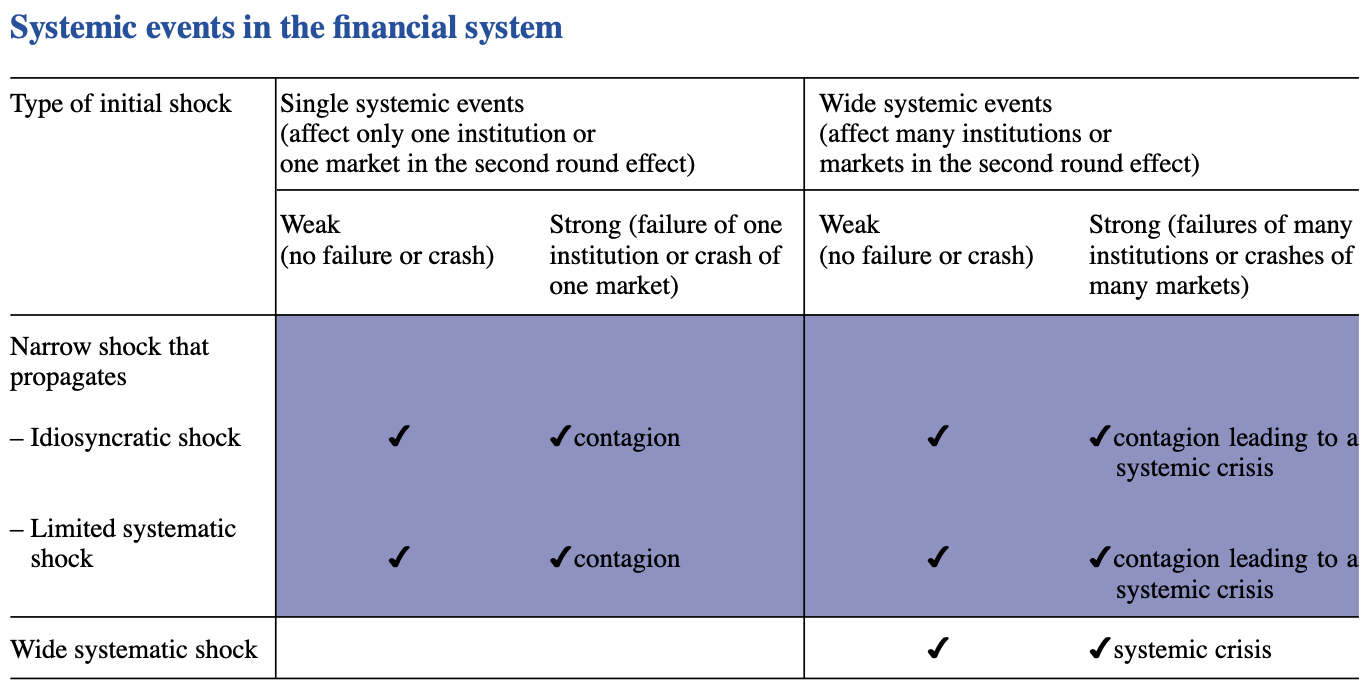
\includegraphics[width=1.0\linewidth]{images/systemic_events.png}
    \caption{\justifying \ding{51} signifie que la combinaison d’événements définie par la cellule constitue un événement systémique. La zone ombrée décrit les cas d’événements systémiques au sens restreint.
Les événements systémiques au sens large incluent également les cellules marquées \ding{51} dans la dernière ligne \citep{debandt2000systemic}.}
    \label{fig:systemic_vents}
\end{figure}

Sur la base de cette terminologie, une crise systémique (au sens restreint ou large) peut être définie comme un événement systémique qui affecte un nombre significatif d’institutions financières ou de marchés de manière forte, compromettant ainsi gravement le bon fonctionnement du système financier ou d’une partie essentielle de celui-ci. Le bon fonctionnement du système financier est ici entendu comme sa capacité à canaliser efficacement l’épargne vers les investissements productifs offrant les meilleurs rendements.\\

Par exemple, une crise financière systémique peut entraîner un rationnement extrême du crédit dans l’économie réelle, phénomène connu sous le nom de credit crunch. La distinction entre événements systémiques et crises systémiques est essentielle, car les mesures de gestion de crise varient en fonction de la nature du choc à l’origine du problème. Un choc idiosyncratique qui risque de provoquer une contagion nécessite une approche différente d’un choc systémique généralisé, qui engendre une déstabilisation simultanée de plusieurs segments du système financier. Cependant, dans la pratique, les situations de crise mêlent souvent chocs globaux et défaillances contagieuses. Par exemple, un ralentissement macroéconomique peut fragiliser des institutions financières, augmentant ainsi le risque de contagion des faillites individuelles. De même, un choc initial peut nécessiter l’effondrement de plusieurs institutions financières pour que la contagion se matérialise pleinement.

\subsubsection{Les symptômes observables du stress financier}

Les périodes de stress financier se manifestent par plusieurs symptômes observables qui traduisent les tensions et dysfonctionnements affectant les marchés financiers et le système bancaire. L’un des premiers signes d’un stress systémique est une volatilité accrue des prix des actifs. En temps normal, les fluctuations des prix des actions, obligations ou devises sont principalement dictées par les fondamentaux économiques et les anticipations des investisseurs. Cependant, en période de forte incertitude, les marchés deviennent plus instables, avec des variations de prix plus marquées et plus fréquentes. Cette volatilité reflète une augmentation des comportements spéculatifs et une réduction de la liquidité, rendant les transactions plus difficiles et amplifiant les mouvements de prix, parfois de manière excessive.\\

Un autre symptôme majeur du stress financier est une chute significative de la valorisation des actifs financiers. Lorsque les investisseurs anticipent une détérioration des conditions économiques ou des défaillances au sein du système financier, ils réévaluent leurs portefeuilles et procèdent à des ventes massives, ce qui entraîne un effondrement des prix des actifs. Ce phénomène a été particulièrement marqué lors de la crise financière de 2008, où la dévalorisation des actifs adossés aux crédits hypothécaires subprime a provoqué une spirale baissière, forçant de nombreuses institutions financières à enregistrer des pertes colossales. Cette perte de confiance généralisée se répercute sur l’ensemble du système financier, aggravant la crise et freinant la reprise économique.\\

Parallèlement, les primes de risque de défaut et de liquidité connaissent une forte augmentation en période de stress systémique. La prime de risque de défaut, qui reflète la probabilité qu’un emprunteur ne puisse pas honorer ses engagements financiers, tend à s’accroître lorsque les perspectives économiques se dégradent ou que la solvabilité des institutions financières est remise en question. Ce phénomène s’observe notamment à travers l’écartement des spreads obligataires, c’est-à-dire l’augmentation de l’écart entre les rendements des obligations d’État considérées comme sûres (telles que les Bunds allemands) et celles des pays ou entreprises perçus comme plus risqués. De même, la prime de liquidité augmente lorsque les investisseurs exigent une compensation plus élevée pour détenir des actifs difficiles à revendre en cas de besoin urgent de liquidités. Cela entraîne des distorsions dans la transmission des signaux de prix et exacerbe l’instabilité des marchés financiers.\\

Le stress systémique représente la manifestation concrète du risque systémique, dont les effets peuvent être dévastateurs pour l’économie si aucune mesure n’est prise pour le contenir. En distinguant les perspectives horizontale et verticale du risque systémique, il est possible d’adopter une approche plus complète pour analyser son impact et identifier les leviers d’intervention les plus efficaces. L’évaluation du risque systémique, notamment via des indicateurs comme le CISS, permet aux décideurs économiques d’anticiper les périodes de tension et d’adopter des politiques monétaires et macroprudentielles adaptées pour limiter la propagation des crises et préserver la stabilité financière.

\subsection{L'indicateur composite de stress systémique}

La stabilité du système financier repose sur l'équilibre des interactions entre les différents segments de marché. Cependant, cet équilibre est régulièrement menacé par des tensions systémiques, amplifiées par l'interconnexion croissante des marchés. Dans ce contexte, des outils d'analyse et de surveillance, tels que le \textit{Composite Indicator of Systemic Stress} (\textit{CISS}), se révèlent essentiels pour comprendre et anticiper les risques systémiques. Conçu pour capturer les signaux de stress financier à travers différents segments, cet indicateur composite intègre les spécificités des marchés actions, des changes, obligataire, des intermédiaires financiers et monétaires, tout en tenant compte de leurs interactions dynamiques.\\

Tout d'abord, il est introduit les fondements du \textit{CISS}, en expliquant son objectif principal : fournir une mesure agrégée du stress systémique tout en capturant les interdépendances entre les segments de marché. Puis, il est exploré son évolution depuis des outils plus sectoriels, tels que le \textit{SovCISS}, jusqu'à sa formulation actuelle, qui intègre des notions de corrélation dynamique entre marchés. Enfin, une attention particulière est portée à la formulation mathématique du \textit{CISS}, mettant en évidence les méthodologies de pondération et de calcul pour cet indicateur.

\subsubsection{Construction de l'indicateur composite de stress systémique}

Le \textit{CISS} est un outil central pour surveiller les tensions systémiques, en offrant une mesure agrégée du stress financier à travers différents segments de marché. Ce paragraphe explore d’abord sa présentation générale, en détaillant son rôle dans l’identification des risques systémiques. Ensuite, l’évolution de cet indicateur depuis le \textit{SovCISS} est discutée, mettant en lumière son passage d’un indicateur centré sur les obligations souveraines à une approche globale intégrant plusieurs segments financiers. Enfin, sa formulation mathématique est présentée, expliquant comment les sous-indicateurs sont normalisés, pondérés et agrégés pour refléter les interconnexions et les corrélations dynamiques entre les marchés. Cette structure vise à clarifier la construction et l’utilité de cet outil dans la gestion des risques financiers.

\subsubsection{Généralités}

Le \textit{CISS} est un outil clé pour la surveillance de la stabilité financière dans les économies modernes, notamment au sein de l'Union européenne. Conçu pour offrir une vue d'ensemble des tensions sur les marchés financiers, cet indicateur composite permet aux régulateurs, en particulier la BCE, d’évaluer le risque systémique en temps réel et d’adapter leurs politiques en conséquence. Le \textit{CISS} a pour objectif principal de détecter les périodes où les tensions financières se manifestent simultanément sur plusieurs segments des marchés, ce qui reflète un risque accru de perturbation de l’ensemble du système financier.\\

Le stress systémique désigne la situation où une instabilité financière locale ou sectorielle s'étend et affecte la stabilité de l'ensemble du système financier. Cette extension peut être provoquée par des interconnexions entre différents segments des marchés financiers, des comportements synchronisés des acteurs économiques, ou encore par des canaux de contagion tels que la liquidité ou la confiance des investisseurs. Lorsqu'une crise se généralise, elle peut perturber le fonctionnement normal des marchés, compromettant ainsi la fourniture de crédit, la stabilité des taux d'intérêt et des taux de change, ainsi que le bon déroulement des institutions financières. Cela peut, à terme, affecter gravement l'économie réelle en réduisant la croissance, en augmentant le chômage et en déstabilisant les secteurs productifs.\\

Dans ce contexte, le \textit{CISS} permet de capter les signaux de tensions financières à travers différents marchés, qu'il s'agisse du marché des actions, des obligations, du marché monétaire ou des changes. En captant ces signaux simultanément, le \textit{CISS} évalue si les tensions dans un segment particulier sont susceptibles de se propager aux autres segments, créant un effet de contagion susceptible de perturber l’ensemble du système financier.\\

Le \textit{CISS} se base sur l'idée que les marchés financiers ne fonctionnent pas en autarcie. Au contraire, ils sont fortement interconnectés, et une crise dans l'un d'eux peut rapidement se propager aux autres via divers canaux. Par exemple, une crise de liquidité sur le marché monétaire peut forcer les banques à vendre massivement leurs actifs financiers, y compris des actions ou des obligations, pour couvrir leurs besoins en liquidité, ce qui augmente la volatilité sur les marchés des actions et obligataires. De même, des fluctuations importantes sur le marché des changes, par exemple une dépréciation rapide d'une monnaie majeure comme l'euro ou le dollar, peuvent provoquer des ajustements significatifs dans les portefeuilles des investisseurs et des entreprises, avec des répercussions sur les marchés actions et obligations. \\

Ce dernier tient compte de ces interconnexions en agrégeant plusieurs sous-indicateurs de stress issus de différents segments du marché. Ces sous-indicateurs mesurent des aspects spécifiques du stress financier, comme la volatilité des prix des actions, les écarts de taux entre les obligations souveraines et les obligations d'entreprises, ou encore les tensions sur les taux interbancaires. En combinant ces informations dans un seul indicateur composite, le CISS offre une mesure globale du risque systémique, tout en accordant une attention particulière aux périodes où les tensions apparaissent simultanément sur plusieurs segments des marchés.\\

Aussi, des caractéristiques majeures de l'indicateur sont qu'il accorde une importance particulière aux corrélations dynamiques entre les différents segments du marché. En période normale, les tensions sur un marché peuvent rester localisées et ne pas se propager aux autres segments. Cependant, en période de crise, ces corrélations tendent à augmenter, ce qui signifie que les chocs dans un segment particulier, comme le marché des actions, ont plus de chances de se transmettre aux autres segments, comme le marché des changes ou le marché monétaire. Le CISS capture cette augmentation des corrélations en attribuant un poids plus important aux périodes où plusieurs marchés sont simultanément sous pression. Ainsi, plus les tensions sont corrélées entre les marchés, plus le CISS augmentera, signalant un risque systémique accru. Cette approche permet de différencier les périodes de stress localisé, qui peuvent ne pas représenter un risque pour l'ensemble du système financier, des périodes de stress systémique, où la contagion entre les segments du marché est plus probable. Cela aide les régulateurs à concentrer leurs efforts sur les périodes où les risques systémiques sont les plus élevés et à ajuster leur politique monétaire ou macroprudentielle en conséquence.\\

L'une des raisons pour lesquelles le CISS est particulièrement précieux pour les régulateurs comme la BCE est qu'il permet de détecter les risques avant qu'ils ne deviennent visibles à travers d'autres indicateurs économiques. En surveillant en permanence l'état des différents segments des marchés financiers, le CISS permet aux régulateurs de réagir de manière proactive aux signes de stress systémique. Cela est particulièrement important dans les économies modernes, où les marchés financiers jouent un rôle essentiel dans l'allocation des ressources et le financement de l'activité économique. De plus, le CISS est un outil précieux pour la politique macroprudentielle, qui vise à prévenir les crises financières avant qu'elles ne se matérialisent. En identifiant les périodes de risque systémique élevé, les régulateurs peuvent prendre des mesures pour renforcer la résilience du système financier, pour illustrer en augmentant les exigences de fonds propres des banques, en imposant des limites sur l'exposition aux risques ou en renforçant les liquidités des institutions financières. L'objectif est de prévenir la contagion des crises financières, de sorte que même en cas de choc sur un segment particulier du marché, le reste du système financier reste suffisamment solide pour absorber ce choc sans s'effondrer.\\

Ainsi, l'utilité de l'indicateur ne se limite pas à la surveillance des marchés financiers. Il joue également un rôle crucial dans la protection de l'économie réelle contre les perturbations financières. Lorsqu'une crise financière devient systémique, elle affecte non seulement les marchés financiers, mais aussi l'économie dans son ensemble. Les entreprises trouvent plus difficile de se financer, les ménages réduisent leurs dépenses en raison des incertitudes économiques, et les banques deviennent plus réticentes à prêter, ce qui aggrave encore la contraction de l'activité économique. En aidant à prévenir les crises systémiques, le CISS contribue indirectement à la stabilité de l'économie réelle, en assurant que les marchés financiers continuent de fonctionner de manière fluide, même en période de tension.\\ 

Après ces généralités il convient de comprendre l'histoire de l'indicateur avant d'aborder son développement.

\subsubsection{Du SovCISS au CISS}

Avant l'introduction du \textit{CISS}, la BCE et d'autres institutions financières utilisaient un autre indicateur appelé \textit{SovCISS} (Sovereign Composite Indicator of Systemic Stress), conçu spécifiquement pour mesurer le stress systémique lié aux marchés des obligations souveraines. Le \textit{SovCISS} a été développé à une époque où les crises de dette souveraine, en particulier celles qui ont frappé la zone euro entre 2010 et 2012, étaient au centre des préoccupations des régulateurs. Cet indice visait à capter les tensions sur les marchés des obligations d'État, en tenant compte des spreads entre les obligations souveraines des pays membres de la zone euro et les obligations dites « sans risque », comme celles de l'Allemagne. En période de crise, les écarts entre les taux d’intérêt des obligations d’États comme ceux de la Grèce ou de l’Italie par rapport à l’Allemagne augmentaient de manière significative, signalant une perte de confiance des investisseurs dans la capacité des gouvernements à honorer leurs dettes.\\

Cependant, bien que le \textit{SovCISS} ait été un outil utile pour comprendre les dynamiques de la crise de la dette souveraine, il est devenu évident qu'un indice uniquement centré sur les obligations souveraines était insuffisant pour mesurer les risques systémiques globaux. Les crises financières récentes, comme celle des subprimes de 2007-2008, ont montré que les crises systémiques ne se limitaient pas à un seul segment, mais résultaient d'une propagation rapide des tensions entre les différents marchés financiers. Ainsi, la BCE a reconnu la nécessité de développer un indicateur plus global, capable de capter les interactions et les tensions simultanées à travers plusieurs segments financiers, tels que les marchés des changes, des actions, des obligations privées, et des banques. C’est dans ce contexte que le \textit{CISS} a été introduit.\\

Le \textit{CISS} surpasse le \textit{SovCISS} en ce qu’il intègre une mesure de la corrélation dynamique entre les segments du marché. Alors que le \textit{SovCISS} se concentrait principalement sur les tensions dans le secteur des obligations souveraines, le \textit{CISS} capte les tensions qui se propagent à travers tous les segments, offrant ainsi une vision plus complète du stress systémique. Il permet non seulement de surveiller les tensions dans chaque segment, mais aussi d’évaluer comment ces tensions interagissent et s’amplifient entre eux. Le passage du \textit{SovCISS} au \textit{CISS} est une évolution dans la manière dont les régulateurs financiers, et en particulier la BCE, appréhendent les crises systémiques : d’une approche sectorielle centrée sur les obligations souveraines à une approche globale qui prend en compte l'ensemble des segments du système financier et leurs interconnexions.

\subsubsection{Le développement du \textit{CISS}}

Les crises financières récentes, notamment la crise des subprimes de 2007-2008, ont montré à quel point les chocs financiers pouvaient rapidement se propager à travers différents segments du système financier, déclenchant ainsi des crises systémiques d’une ampleur sans précédent. Avant la création du \textit{CISS}, les outils de surveillance disponibles, bien qu'utiles pour comprendre certains aspects des marchés financiers, étaient trop fragmentés et ne permettaient pas de saisir pleinement l'ampleur ni la portée des risques systémiques. Ces outils étaient principalement axés sur des indicateurs spécifiques à chaque segment, tels que les taux interbancaires, les spreads obligataires ou la volatilité des marchés actions, sans intégrer de manière adéquate les interconnexions entre les différents segments. Cela créait une lacune dans la surveillance globale des risques financiers, notamment en ce qui concerne l’anticipation de crises systémiques.\\

L'indicateur répond à ce besoin en fournissant une mesure agrégée du stress systémique, capable de capturer les tensions qui surviennent simultanément dans plusieurs secteurs du système financier. Ce cadre analytique plus intégré s’est révélé essentiel après la crise des subprimes, une période où les indicateurs traditionnels avaient échoué à identifier les signes avant-coureurs d’une crise mondiale. La crise de 2007-2008 a particulièrement mis en lumière les insuffisances des indicateurs sectoriels pour surveiller et anticiper les risques financiers. Les outils utilisés à cette époque étaient trop compartimentés, focalisés sur des segments isolés des marchés, ce qui empêchait de saisir l'ampleur des interconnexions et de l’effet de contagion qui allait finalement provoquer un effondrement général du système financier. Le CISS a été conçu pour combler cette lacune en offrant une vue d’ensemble des risques systémiques en agrégeant les tensions dans les principaux segments financiers : le secteur bancaire, les marchés obligataires, les marchés des actions, les marchés des changes, et d’autres segments financiers clés.\\

Son développement repose sur des concepts tirés de la théorie des portefeuilles, développée par Harry Markowitz dans les années 1950. Cette théorie met en évidence le rôle crucial de la diversification pour optimiser un portefeuille d’actifs en termes de rentabilité maximale et de risque minimal. De la même manière, cet indicateur applique ce principe à la gestion du risque systémique en combinant plusieurs segments du système financier tout en tenant compte des corrélations temporelles entre eux. Chaque segment est susceptible de subir des chocs qui peuvent se propager aux autres segments par le biais de multiples canaux de transmission. L’indicateur reflète donc non seulement les tensions dans chaque segment, mais aussi la manière dont ces tensions interagissent et s’amplifient à travers les interconnexions systémiques. C'est donc un outil global particulièrement pertinent pour mesurer le risque systémique à un instant donné.\\

En outre, cet indicateur permet de surveiller en temps réel les tensions qui se manifestent dans les différents segments du système financier. Cela en fait une métrique particulièrement précieuse pour les banques centrales et les autorités financières, car il leur offre la possibilité de détecter les signes précoces de crises potentielles et de mettre en place des mesures préventives pour stabiliser le système. En identifiant les périodes de stress simultané sur plusieurs segments, il permet d’anticiper les crises avant qu’elles ne deviennent trop graves et d’intervenir de manière proactive. Il constitue également un outil d’analyse rétrospective, permettant d’examiner les crises passées et d’évaluer les niveaux de stress atteints durant ces périodes critiques. Il est donc possible d’établir des comparaisons entre différentes crises financières et d’en analyser les dynamiques propres, facilitant ainsi l’évaluation des politiques et des mesures mises en place pour répondre à ces crises.\\

Par exemple, en comparant les niveaux atteints durant la crise des subprimes à ceux observés pendant la crise de la dette souveraine en Europe, il est possible d’évaluer l’efficacité des réponses monétaires et fiscales appliquées dans chacun de ces cas. Ce type d’analyse comparative permet également de tirer des enseignements utiles pour la gestion des futures crises. Une analyse approfondie des dynamiques de chaque crise aide les régulateurs à mieux comprendre les mécanismes de propagation des tensions financières et à ajuster leurs outils en conséquence.\\

Cet indicateur agit également comme un outil de rétroaction particulièrement utile pour les décideurs politiques et monétaires. Après une intervention de la banque centrale, une baisse significative de l’indicateur signalerait que les mesures prises ont effectivement contribué à réduire les tensions dans le système financier. Cette capacité d’évaluer les réponses politiques et monétaires en temps réel confère à cet outil un rôle unique dans la gestion des crises financières. Contrairement aux indicateurs traditionnels qui ne captent que des aspects isolés du marché, il permet une vision plus holistique des risques, facilitant ainsi des réponses politiques plus efficaces et mieux ciblées.\\

Il est décomposé en cinq indices principaux, chacun représentant un segment majeur du marché financier, tels que le secteur bancaire, les marchés obligataires, les marchés des actions, les marchés des changes et les autres segments financiers pertinents. Chacun de ces indices est ensuite subdivisé en sous-indices qui capturent des aspects spécifiques de leurs segments respectifs, comme la volatilité des actions, les spreads des obligations souveraines ou les tensions sur les taux interbancaires. Cette structure hiérarchisée permet à l’outil d’offrir une vision à la fois large et détaillée des tensions financières, tout en tenant compte des interdépendances entre les segments. L’agrégation de ces indices, en tenant compte des corrélations entre eux, permet de générer un indicateur composite qui mesure le niveau global de risque systémique auquel est confronté le système financier.\\

L’innovation apportée par cet indicateur réside donc dans sa capacité à offrir une mesure intégrée et dynamique des risques financiers. Contrairement aux approches traditionnelles, qui se concentrent sur l’intensité des tensions dans des segments spécifiques, il prend en compte la propagation et la diffusion de ces tensions à travers l’ensemble du système financier. Cela permet aux régulateurs de mieux comprendre la manière dont les chocs financiers se propagent entre les différents segments et d’anticiper l’apparition de crises systémiques. En intégrant à la fois l’intensité des tensions et leur diffusion à travers le système, cet outil devient central pour la gestion et l’anticipation des crises financières.

%Graphique 

\subsubsection{Formulation mathématique du \textit{CISS}}

Le \textit{CISS} repose sur cinq indices, chacun étant lui-même subdivisé en plusieurs sous-indices. Ces indices principaux sont pondérés en fonction de leur importance relative, avec des coefficients spécifiques attribués à chaque sous-indice, ce qui permet d'obtenir une mesure globale du risque systémique. Les poids attribués aux indices déterminent leur influence sur le calcul final du \textit{CISS}. La construction mathématique suivante est reprise de \citep{hollo2012ciss}.

\begin{enumerate}
    \item  30\% pour le marché intermédiaire
    \item 25\% pour le marché des actions 
    \item 15\% pour le marché obligataire 
    \item 15\% pour le marché monétaire
    \item 15\% pour le marché des changes
\end{enumerate}

Pour chaque segment de marché, trois indicateurs de stress financier sont sélectionnés, notés \( x_{t,i,j} \). Soit un ensemble de valeurs observées \( x_1, x_2, \dots, x_n \) pour un indicateur spécifique. On ordonne ces valeurs de telle sorte que \( x_{[1]} \leq x_{[2]} \leq \dots \leq x_{[n]} \), où \( x_{[r]} \) représente le \( r \)-ième ordre de valeur. De plus,

\begin{itemize}
    \item \( t \) représente le temps,
    \item \( i \) indique le segment de marché (\( i = 1, 2, 3, 4, 5 \) pour les marchés monétaires, obligations, actions, intermédiaires financiers, et changes),
    \item \( j \) correspond à chaque indicateur spécifique dans le segment (\( j = 1, 2, 3 \)).
\end{itemize}

Ces indicateurs sont normalisés en utilisant leur fonction de distribution cumulative empirique \( F(x_{t,i,j}) \), ce qui donne le score normalisé :
\begin{equation}
z_{t,i,j} = F(x_{t,i,j}) = \frac{r}{n}
\end{equation}
où \( r \) est le rang de \( x_{t,i,j} \) dans un ensemble de \( n \) observations, ordonnées de manière croissante. La transformation est mise à jour de manière récursive pour chaque nouvelle observation \( T \) :
\begin{equation}
z_{T,i,j} = F_{T}(x_{T,i,j}) = \frac{r}{T}
\end{equation}

Par la suite, pour chaque segment de marché \( i \), un sous-indice \( s_{t,i} \) est construit en prenant la moyenne arithmétique des trois indicateurs normalisés :
\begin{equation}
s_{t,i} = \frac{1}{3} \sum_{j=1}^{3} z_{t,i,j}
\end{equation}

Enfin, les cinq sous-indices sont agrégés dans un indicateur composite \( CISS_t \) en utilisant des poids \( w_i \) représentant leur importance pour l'activité économique réelle. Le vecteur de poids est \( w = [0.15, 0.15, 0.25, 0.30, 0.15] \). Le CISS est calculé en tenant compte des corrélations dynamiques entre les segments :
\begin{equation}
CISS_t = \left( w \circ s_t \right)^T C_t \left( w \circ s_t \right) = \sum_{i=1}^{5} \sum_{j=1}^{5} w_i w_j s_{t,i} s_{t,j} \rho_{t,ij}
\end{equation}
où \( w \circ s_t \) représente le produit de Hadamard (élément par élément) entre le vecteur de poids \( w \) et le vecteur des sous-indices \( s_t = [s_{t,1}, s_{t,2}, s_{t,3}, s_{t,4}, s_{t,5}] \), et \( C_t \) est la matrice de corrélation des sous-indices.\\

Aussi, la matrice de corrélation \( C_t \) est une matrice symétrique \( 5 \times 5 \), où chaque élément \( \rho_{t,ij} \) représente la corrélation entre les sous-indices \( s_{t,i} \) et \( s_{t,j} \) :

\begin{equation}
C_t = \begin{bmatrix}
1 & \rho_{t,12} & \rho_{t,13} & \rho_{t,14} & \rho_{t,15} \\
\rho_{t,12} & 1 & \rho_{t,23} & \rho_{t,24} & \rho_{t,25} \\
\rho_{t,13} & \rho_{t,23} & 1 & \rho_{t,34} & \rho_{t,35} \\
\rho_{t,14} & \rho_{t,24} & \rho_{t,34} & 1 & \rho_{t,45} \\
\rho_{t,15} & \rho_{t,25} & \rho_{t,35} & \rho_{t,45} & 1 \\
\end{bmatrix}
\end{equation}

Les éléments de la matrice \( C_t \) sont calculés en fonction des covariances \( \sigma_{t,ij} \) et des écarts-types des sous-indices respectifs \( \sigma_{t,i} \) et \( \sigma_{t,j} \) :

\begin{equation}
\rho_{t,ij} = \frac{\sigma_{t,ij}}{\sqrt{\sigma_{t,i}^2 \cdot \sigma_{t,j}^2}}
\end{equation}

Les covariances et variances sont calculées de manière récursive avec des moyennes mobiles exponentielles :

\begin{equation}
\sigma_{t,i}^2 = \lambda \sigma_{t-1,i}^2 + (1 - \lambda) \tilde{s}_{t,i}^2
\end{equation}

\begin{equation}
\sigma_{t,ij} = \lambda \sigma_{t-1,ij} + (1 - \lambda) \tilde{s}_{t,i} \tilde{s}_{t,j}
\end{equation}

où \( \lambda \) est un paramètre de lissage, typiquement autour de 0.93 \citep{hollo2012ciss}, et \( \tilde{s}_{t,i} \) est le sous-indice centré autour de sa moyenne historique.\\

Le stress systémique constitue une menace majeure pour la stabilité du système financier européen, amplifiée par les interconnexions croissantes entre les segments de marché et les institutions financières. Sa compréhension nécessite une analyse fine des dynamiques de contagion, des niveaux d'intensité des événements systémiques, ainsi que des symptômes observables lors des épisodes de crise. Dans ce contexte, l’indicateur composite de stress systémique (\textit{CISS}) s’impose comme un outil de surveillance particulièrement pertinent. Il permet ainsi d’anticiper les phases critiques et d’ajuster les réponses politiques en conséquence. Toutefois, la surveillance des risques systémiques ne saurait se limiter à une lecture technique des indicateurs. Elle nécessite également une réflexion sur les leviers d’action mobilisables pour limiter la propagation des crises. Parmi ces leviers, la politique monétaire — et en particulier la forward guidance — joue un rôle croissant dans la gestion des anticipations et des tensions sur les marchés financiers.\\

C’est pourquoi il est ensuite proposé d’examiner les interactions entre la forward guidance et le stress systémique, en analysant dans quelle mesure une communication stratégique efficace de la banque centrale peut contribuer à prévenir, amortir ou au contraire amplifier les épisodes de turbulence financière.

\section{Stress systémique et forward guidance}

L’analyse du lien entre la forward guidance et le stress systémique constitue un champ d’étude encore relativement peu exploré, malgré l’importance croissante de ces deux concepts dans la politique monétaire moderne. La forward guidance est largement reconnue comme un instrument central permettant aux banques centrales d’influencer les anticipations des agents économiques et de renforcer la transmission de la politique monétaire. Parallèlement, le stress systémique, qui résulte de perturbations majeures affectant l’ensemble du système financier, représente une préoccupation majeure pour les autorités monétaires et macroprudentielles. Toutefois, la manière dont la forward guidance interagit avec le stress systémique demeure peu étudiée dans la littérature. Alors que de nombreuses recherches ont porté sur le rôle des taux d’intérêt et des mesures non conventionnelles dans la stabilité financière, peu d’études se sont focalisées sur l’impact spécifique des stratégies de communication des banques centrales dans la prévention ou l’amplification des tensions financières. Dans un contexte où la BCE et d’autres institutions monétaires s’appuient de plus en plus sur la forward guidance pour stabiliser les marchés et orienter les anticipations, il apparaît essentiel de comprendre dans quelle mesure cet outil peut influencer le niveau de stress systémique. La forward guidance peut-elle réellement réduire les tensions financières en apportant de la visibilité aux investisseurs et aux intermédiaires financiers ? Ou, au contraire, peut-elle accroître le stress systémique en cas de perte de crédibilité ou de mauvaise interprétation par les marchés ? Ce paragraphe propose d’analyser ces questions en approfondissant les interactions entre ces deux dynamiques fondamentales.L’examen de cette relation se fera en trois étapes. Tout d’abord, l’impact de la forward guidance sur le stress systémique fera l'objet d'une étude, en mettant en lumière les mécanismes par lesquels cet outil peut contribuer à atténuer ou, au contraire, à exacerber les tensions sur les marchés financiers. Il analysera notamment comment une forward guidance claire et crédible peut jouer un rôle stabilisateur en période de crise, en réduisant l’incertitude et en limitant la volatilité des marchés. Toutefois, les risques liés à une mauvaise gestion de la forward guidance seront également explorés, notamment en ce qui concerne la perte de crédibilité des banques centrales et les distorsions de marché qu’une politique mal calibrée peut engendrer.Ensuite, l’interaction entre la forward guidance et la régulation macroprudentielle sera abordée. Il sera examiné dans quelle mesure la forward guidance peut compléter ou entrer en conflit avec les mesures de stabilité financière mises en place par les autorités macroprudentielles. La nécessité d’une coordination entre ces deux approches est mise en évidence, afin d’éviter que les effets de la forward guidance ne compromettent l’efficacité des mesures prudentielles, et inversement. Enfin, une attention particulière portera sur les limites et les défis d’une coordination insuffisante entre la politique monétaire et la régulation macroprudentielle. Cela montrera comment une communication mal alignée avec les mesures macroprudentielles peut générer de l’incertitude et accroître le stress systémique, notamment lorsque les signaux envoyés aux marchés financiers deviennent contradictoires. À travers cette analyse, sont ainsi mises en évidence les implications de la forward guidance pour la stabilité du système financier et les précautions à prendre pour éviter qu’elle ne devienne une source supplémentaire de stress systémique

\subsection{Impact de la forward guidance sur le stress systémique}

La forward guidance, en influençant les anticipations des agents économiques, peut aussi jouer un rôle dans la réduction ou l’amplification du stress systémique au sein du système financier. Le stress systémique, souvent provoquées par des crises de liquidité, des faillites bancaires ou des pertes de confiance généralisées dans le système financier. Dans ce contexte, la capacité des banques centrales à ancrer efficacement les anticipations via la forward guidance peut contribuer à limiter les risques de propagation des crises.

\subsubsection{La forward guidance comme outil de réduction du stress systémique}

Une forward guidance claire, crédible et bien communiquée peut jouer un rôle stabilisateur en période de stress systémique. L’un des principaux canaux par lesquels elle agit est la réduction de l’incertitude macroéconomique et financière. En fournissant aux agents économiques des indications précises sur l’orientation future des taux d’intérêt et des conditions monétaires, la forward guidance permet d’ancrer les anticipations et de limiter la volatilité excessive des marchés \citep{woodford2012}).\\

Par exemple, lors de la crise des dettes souveraines en 2012, la déclaration de Mario Draghi affirmant que la BCE ferait "whatever it takes" pour préserver l’euro a eu un effet immédiat de réduction du stress systémique. Cette simple communication a permis de restaurer la confiance des investisseurs et d'éviter une fragmentation accrue des marchés obligataires de la zone euro \citep{Acharya2015}. La forward guidance peut donc jouer un rôle similaire à celui d’un pare-feu psychologique, en signalant aux marchés que la banque centrale est prête à intervenir pour stabiliser le système financier.\\

De plus, en périodes de crises financières, la forward guidance peut atténuer le risque de contagion en fixant un cap clair sur l’évolution future des conditions monétaires. Une politique monétaire imprévisible ou perçue comme hésitante peut engendrer des comportements procycliques, où les investisseurs réduisent leur exposition au risque de manière excessive, aggravant ainsi la crise. En maintenant des engagements crédibles sur la trajectoire des taux d’intérêt, la forward guidance permet d’éviter des ventes massives d’actifs et un durcissement excessif des conditions financières \citep{swanson2021}.

\subsubsection{Risques et effets indésirables de la forward guidance sur le stress systémique}

Si la forward guidance peut être un instrument stabilisateur, elle présente aussi des risques potentiels qui peuvent, sous certaines conditions, aggraver le stress systémique. L’un des principaux dangers réside dans une perte de crédibilité de la banque centrale. Lorsque les marchés perçoivent que la forward guidance n’est pas suivie d’actions cohérentes, cela peut créer un climat d’incertitude accru, qui amplifie la volatilité des marchés financiers.\\

Un exemple marquant de ce phénomène est le "Taper Tantrum" de 2013, où l’annonce prématurée d’un ralentissement des achats d’actifs par la Réserve fédérale américaine (Fed) a provoqué une flambée des taux d’intérêt à long terme et un effondrement des marchés émergents. Cette réaction excessive s’explique par un changement soudain de forward guidance, mal anticipé par les investisseurs \citep{gürkaynak2015}. Cet épisode illustre comment une mauvaise gestion des attentes peut engendrer une crise de liquidité et de confiance, exacerbant ainsi le stress systémique.\\

Un autre problème réside dans le risque de distorsions financières et de prise de risque excessive. Une forward guidance trop accommodante, en signalant un maintien prolongé des taux bas, peut inciter les investisseurs à rechercher des rendements plus élevés en prenant des risques excessifs. Ce phénomène, connu sous le nom de "search for yield", peut gonfler des bulles financières et fragiliser le système bancaire en période de resserrement monétaire. Par exemple, la période prolongée de taux bas après la crise financière de 2008 a favorisé une accumulation de dettes privées et une montée des valorisations boursières, augmentant la vulnérabilité du système financier en cas de choc externe.

\newpage

Le stress systémique résulte souvent d’interactions entre déséquilibres macroéconomiques, comportements. Alors, il est essentiel d’examiner comment la forward guidance peut s’articuler avec d’autres outils de gestion du risque systémique, notamment la régulation macroprudentielle.

\subsection{Interactions entre forward guidance et régulation macroprudentielle dans la gestion du stress systémique}

Dans ce paragraphe il est montré l’interaction entre la forward guidance et la régulation macroprudentielle dans la gestion du stress systémique. La complémentarité entre ces deux outils permet de stabiliser les anticipations des marchés et de limiter les déséquilibres financiers liés à des politiques monétaires accommodantes prolongées.  Cependant, en l’absence de coopération étroite, des conflits d’objectifs peuvent apparaître, augmentant l’incertitude et la volatilité des marchés. L’étude de ces interactions est donc essentielle pour affiner la communication des banques centrales et renforcer la stabilité financière.

\subsubsection{La complémentarité entre forward guidance et régulation macroprudentielle}

La forward guidance, en tant qu'outil central de communication des banques centrales, joue un rôle déterminant en influençant les anticipations des marchés financiers. Son objectif est de clarifier les intentions futures en matière de politique monétaire afin d’orienter les attentes des acteurs économiques vers des scénarios souhaités par les autorités monétaires. Cependant, cette stratégie doit nécessairement interagir de manière étroite avec la régulation macroprudentielle, dont la finalité principale est de limiter l'accumulation de risques systémiques susceptibles de déstabiliser l'économie globale. Selon les travaux pionniers de \citep{BorioZhu2012}, la coordination étroite entre la forward guidance et les instruments de régulation macroprudentielle permet une gestion plus efficace du stress systémique. En effet, une politique macroprudentielle rigoureuse peut renforcer la crédibilité et l'efficacité de la forward guidance en rassurant les acteurs économiques sur le fait que les risques financiers demeureront maîtrisés, même en situation prolongée de taux d'intérêt très bas. \citep{FilardoHofmann2014} soulignent à cet égard que la confiance dans la stabilité financière rend les anticipations des acteurs économiques plus robustes, facilitant ainsi l'atteinte des objectifs de la politique monétaire. \citep{GalatiMoessner2018} approfondissent cette analyse en montrant que la combinaison stratégique de la forward guidance avec des politiques macroprudentielles permet une stabilisation accrue des anticipations des marchés financiers. Cette combinaison réduit significativement les risques de formation de bulles spéculatives, lesquelles constituent une menace importante pour la stabilité financière à long terme. Ainsi, en évitant les excès d'optimisme ou de pessimisme sur les marchés, cette coordination améliore considérablement l'efficacité globale de la politique monétaire. Par ailleurs, \citep{Smets2014} insiste sur l'importance d'une coordination proactive entre ces deux politiques. Une telle approche anticipative permet aux banques centrales et aux autorités macroprudentielles d’ajuster de manière optimale les anticipations des agents économiques, minimisant ainsi l'incertitude et la volatilité financière qui peuvent surgir lors de périodes prolongées de politique monétaire accommodante. En agissant conjointement, les autorités monétaires et prudentielles sont ainsi mieux placées pour gérer efficacement les périodes complexes où l’équilibre économique est particulièrement sensible aux variations d’anticipations des marchés.

\subsubsection{Risques et limites d’une coordination insuffisante}

Cependant, l’absence d’une coordination adéquate entre forward guidance et régulation macroprudentielle peut générer des conflits et réduire significativement l’efficacité des politiques mises en œuvre. \citep{farhi2016} soulignent explicitement que, sans une coopération étroite, les objectifs de stabilisation financière peuvent entrer en conflit direct avec ceux de la politique monétaire, particulièrement lorsque des taux d'intérêt bas prolongés incitent les acteurs financiers à adopter des comportements de prise de risque excessifs. Ce phénomène peut alors conduire à une accumulation dangereuse de déséquilibres financiers, menaçant la stabilité du système économique. \citep{claessens2013} préconisent ainsi une approche intégrée impliquant un échange actif et continu d'informations entre les banques centrales et les autorités macroprudentielles. Selon eux, une telle coordination permet d’éviter efficacement les effets secondaires indésirables des politiques individuelles. Par exemple, elle réduit les risques de formation de bulles spéculatives ou de surchauffe des marchés, tout en limitant les comportements risqués encouragés par des conditions monétaires accommodantes prolongées. Par ailleurs, \citep{rey2015} met en garde contre les conséquences potentiellement graves d’une coordination insuffisante. Des politiques contradictoires ou mal coordonnées peuvent en effet générer des signaux confus pour les marchés financiers, augmentant ainsi l’incertitude et aggravant le stress systémique. Cette confusion peut conduire à une volatilité accrue et à une instabilité financière qui, à son tour, nuit gravement à la réalisation des objectifs économiques globaux. Plus récemment, \citep{linta2024} met en évidence l'importance de la crédibilité dans l'efficacité de la forward guidance, soulignant que cette crédibilité dépend en grande partie d'une des votes en conseil des gouverneurs.\\

Dans ce cadre, étudier spécifiquement l'impact de la forward guidance sur le stress systémique est important pour les régulateurs. Une meilleure compréhension de cet impact permettrait aux décideurs publics d'affiner leur communication et de calibrer précisément leurs messages afin de réduire l’incertitude sur les marchés financiers, limitant ainsi les risques d’instabilité et de crises systémiques potentielles. Également, en analysant précisément les mécanismes par lesquels la forward guidance influence les anticipations des acteurs économiques, les régulateurs pourraient mieux anticiper et contrôler les comportements de prise de risque excessifs qui accompagnent souvent les périodes prolongées de politique monétaire accommodante. Enfin, une recherche approfondie sur ce sujet pourrait également fournir des orientations précieuses quant à l’articulation optimale entre la forward guidance et les mesures macroprudentielles, permettant ainsi aux régulateurs de mieux coordonner ces politiques et d’améliorer globalement l’efficacité de leur gestion du risque systémique.

\newpage

Dans ce chapitre, l'analyse du lien entre stress systémique et forward guidance met en évidence le rôle central que joue la communication des banques centrales dans la stabilité financière. En influençant les anticipations des agents économiques, la forward guidance peut à la fois réduire l’incertitude et limiter la volatilité des marchés, contribuant ainsi à la prévention des crises financières. Cependant, son efficacité repose sur deux piliers fondamentaux : la crédibilité des engagements des banques centrales et la cohérence des signaux envoyés aux marchés. Une forward guidance bien calibrée peut atténuer les tensions financières en ancrant les anticipations et en stabilisant les conditions monétaires, comme l’a illustré la réponse de la BCE lors de la crise des dettes souveraines.Toutefois, des risques demeurent. Une communication inadaptée ou une perte de crédibilité peuvent accentuer le stress systémique en créant de l’incertitude et en amplifiant les mouvements de marché. De plus, l’effet de la forward guidance sur les comportements d’investissement peut, en période prolongée de taux bas, favoriser des prises de risque excessives et la formation de bulles financières, augmentant ainsi la vulnérabilité du système financier.\\

L’interaction entre la forward guidance et la régulation macroprudentielle apparaît dès lors comme un levier essentiel pour assurer une gestion efficace du stress systémique. Une coordination renforcée entre ces deux outils permettrait de stabiliser les anticipations tout en limitant l’accumulation des déséquilibres financiers. À l’inverse, une absence de coordination ou des signaux contradictoires entre politique monétaire et régulation macroprudentielle risquent de fragiliser davantage le système financier, compromettant ainsi l’objectif de stabilité macroéconomique. Ainsi, la compréhension approfondie des interactions entre stress systémique et forward guidance constitue un enjeu majeur pour les banques centrales et les régulateurs financiers. Face à des crises financières de plus en plus interconnectées, il apparaît essentiel d’affiner les outils de communication monétaire et d’assurer une complémentarité efficace avec les mesures macroprudentielles. L’analyse du stress systémique et de ses déterminants, notamment à travers des indicateurs comme le \textit{CISS}, doit ainsi s’intégrer pleinement dans l’élaboration des stratégies monétaires et prudentielles. En définitive, une forward guidance efficace et cohérente avec les objectifs de stabilité financière représente un instrument puissant pour prévenir les crises et renforcer la résilience du système financier européen.\\

Afin d'étudier correctement le rôle de la forward guidance dans la dynamique du stress systémique, il est indispensable de modéliser rigoureusement ses mécanismes de transmission et ses effets différés sur les marchés financiers. En effet, les annonces de politique monétaire ne produisent pas des réactions instantanées, linéaires ou uniformes : leur impact dépend fortement des anticipations, des conditions de marché préexistantes, et peut se manifester de manière progressive ou différenciée selon les canaux de transmission. Le caractère temporel, non linéaire et parfois latent de ces réactions économiques appelle à mobiliser des outils capables de capturer des dépendances de long terme, de modéliser des régimes dynamiques sous-jacents. Le second chapitre se consacre ainsi à l’exploration des architectures neuronales avancées les plus pertinentes pour cette tâche afin de mémoriser et représenter les signaux de politique monétaire, dans le but de mesurer leur effet sur les dynamiques de stress systémique.
\chapter{Méthodologies d'analyse par\\ Deep Learning}
\minitoc

La modélisation du langage naturel a connu, au cours des deux dernières décennies, une transformation radicale sous l’effet des avancées en apprentissage profond. Cette révolution est particulièrement significative dans les domaines où l’interprétation du langage joue un rôle dans la dynamique des marchés et des anticipations, comme c’est le cas pour les discours de politique monétaire. Les progrès récents dans les architectures neuronales ont non seulement permis des performances importantes dans la compréhension automatique des textes, mais ils ont également modifié la manière dont les économistes peuvent modéliser l’impact du langage institutionnel sur les variables macroéconomiques et financières \citep{vaswani2017attention, devlin2018bert}. Dans ce contexte, qui vise à quantifier et analyser les effets de la forward guidance de la Banque centrale européenne sur le stress systémique via les indicateurs comme le CISS, il est nécessaire de s’appuyer sur des outils de modélisation capables de capturer la complexité linguistique des discours tout en conservant une structure temporelle compatible avec les dynamiques économiques. Cela nécessite une compréhension approfondie des architectures neuronales modernes, à la fois sur le plan théorique, algorithmique et empirique. Ce chapitre se donne pour objectif de dresser une typographie structurée des principales architectures de Deep Learning appliquées au traitement du langage naturel (NLP), en mettant l’accent sur trois familles majeures : les perceptrons multicouches (MLP) en guise d'introduction, les Transformers, et les modèles d’espace d’état linéaire à mémoire longue (LSSL), dont Mamba et Llamba représentent les dernières avancées. Les MLP (Multilayer Perceptrons) constituent la fondation du Deep Learning. Dès les travaux pionniers sur le perceptron de \citep{rosenblatt1957perceptron}, puis son extension à des architectures à plusieurs couches dans les années 1980-90 grâce à la rétropropagation \citep{rumelhart1986learning, lecun1998gradient}, les réseaux de neurones ont progressivement acquis la capacité d’approximer des fonctions complexes dans des espaces de grande dimension \citep{cybenko1989approximation}. Bien que leur usage dans le traitement du langage soit limité par leur nature statique et leur absence de mémoire séquentielle, les MLP constituent une base indispensable pour comprendre les représentations non linéaires apprises par les réseaux profonds. Le véritable tournant a eu lieu avec l’introduction des Transformers par \citep{vaswani2017attention}, qui a proposé une architecture novatrice basée uniquement sur le mécanisme d’attention, sans aucune récursivité ni convolution. Le modèle s’affranchit des limitations des RNN en permettant un accès direct à l’ensemble de la séquence, ce qui facilite l’apprentissage de dépendances à long terme tout en permettant une parallélisation efficace. Les Transformers ont rapidement dominé le domaine du NLP, comme en témoignent leurs incarnations dans BERT \citep{devlin2018bert}, GPT \citep{radford2018gpt1, radford2019gpt2, brown2020gpt3}, T5 \citep{raffel2020t5} et plus récemment dans des variantes adaptées à des contextes computationnels plus contraints \citep{gu2022trainhippo, qin2023transnormerllm}. Ces architectures s’appuient sur des fondements mathématiques profonds : la structure attentionnelle peut être interprétée comme une forme de projection contextuelle dans un espace de haute dimension, où chaque mot est représenté conditionnellement aux autres via des poids appris \citep{cho2014learning}. Sur le plan économique, cela permet de capturer finement les nuances contextuelles des discours monétaires, comme les changements de ton, les anticipations implicites ou encore les effets de signaux faibles présents dans les discours de forward guidance. Malgré leur puissance, les Transformers souffrent de deux limitations importantes : leur coût quadratique en mémoire et en calcul, et leur traitement fondamentalement discret du temps, ce qui peut poser problème pour la modélisation de phénomènes économiques continus ou multi-échelles. Pour répondre à ces limites, une nouvelle classe de modèles s’est récemment imposée : les Linear State Space Models (LSSM), qui modélisent explicitement la dynamique temporelle à l’aide d’équations différentielles linéaires ou de systèmes dynamiques en temps continu \citep{gu2021combining, gu2023mamba}. Les architectures de type Mamba introduisent un formalisme mixte, combinant l’efficacité de la convolution (avec des noyaux appris en temps continu) et la structure modulaire des états cachés issus des systèmes linéaires. Elles permettent ainsi d’intégrer efficacement des signaux à longue portée sans recourir à l’attention, tout en maintenant une expressivité comparable. La variante Llamba \citep{bick2025llamba}, récemment introduite, va plus loin en remplaçant les convolutions standards par des modules de type Linear Recurrent Operator, offrant une expressivité et une capacité de compression temporelle plus fine. Afin de pouvoir appliqué l'impact de la Forward Guidance sur le CISS il sera finalement developpé des méthodes de Deep Learning appliquées aux séries temporelles. Les réseaux à mémoire longue de type Long Short-Term Memory seront présentés. Proposés initialement par \citep{hochreiter1997long}, ces réseaux se sont imposés comme une solution performante pour la capture des dépendances temporelles de longue portée. Leur structure interne, reposant sur des mécanismes de portes et des cellules mémoire, a permis d’améliorer la prédiction dans des environnements où les effets différés et les transmissions lentes, tels que ceux associés à la politique monétaire \citep{qin2023transnormerllm}. Ensuite, les autoencodeurs avec distance de Wasserstein seront étudiés. Introduits par \citep{tolstikhin2018wasserstein}, ces modèles se fondent sur une approche de transport optimal de l’encodage et de la génération de données. En permettant une représentation latente structurée des séries temporelles, les WAE ont été utilisés pour l’extraction de régimes cachés, la compression de l’information et la génération de trajectoires économiques plausibles dans des cadres contrefactuels \citep{chung2015recurrent, fraccaro2016sequential}.  L’ensemble de ces modèles sera analysé tant du point de vue de leur architecture que de leurs fondements mathématiques et algorithmiques. Tous ces modèles sont alors pertinents pour la modélisation du stress systémique, tel que mesuré par l’indicateur CISS.

\section{Fondamentaux des réseaux de neurones}

Le deep learning repose en grande partie sur la formalisation mathématique et l'efficacité empirique des réseaux de neurones artificiels (RNA), qui sont devenus les pionniers de la modélisation moderne des données. Inspirés du fonctionnement biologique des neurones dans le cerveau humain \citep{mcculloch1943logical}, ces modèles permettent de capturer des relations non linéaires entre variables grâce à une succession de transformations affines et d’activations non linéaires. Cette capacité d’approximation, combinée à une grande flexibilité architecturale, en fait des instruments particulièrement puissants pour l’analyse et la prédiction dans des contextes hétérogènes, allant de la reconnaissance visuelle à la modélisation de séries temporelles \citep{lecun2015deep, schmidhuber2015deep}. L’efficacité des RNA repose non seulement sur leur structure modulaire, mais également sur les algorithmes d’optimisation numériques qui permettent l’ajustement de leurs paramètres internes à partir des données. Ces méthodes exploitent les gradients de la fonction de perte pour guider l’apprentissage, en s’appuyant sur des principes mathématiques et des techniques informatiques \citep{rumelhart1986learning, bottou2010large}. Le présent paragraphe a pour objectif d’introduire les fondements théoriques essentiels à la compréhension des réseaux de neurones profonds. Il est consacrée, tout d'abord, à la structure interne des RNA : elle détaille la modélisation d’un neurone artificiel, les fonctions d’activation couramment utilisées, ainsi que la construction des architectures multicouches de type perceptron (MLP). En particulier, le théorème d’universalité de l’approximation \citep{cybenko1989approximation, hornik1989multilayer} sera mis en lumière, en tant que justification théorique centrale de la capacité d’approximation des MLP. Le paragraphe poursuit sur les mécanismes d’apprentissage et d’optimisation. Elle présente en détail les algorithmes de descente de gradient et leurs variantes (stochastique, mini-batch, momentum, Adam), ainsi que l’algorithme fondamental de rétropropagation du gradient \citep{lecun1998gradient}, qui permet de calculer efficacement les dérivées nécessaires à l’entraînement des réseaux. Enfin, les principales stratégies de régularisation (telles que le dropout \citep{srivastava2014dropout}, la normalisation de batch \citep{ioffe2015batch}, ou encore l’arrêt anticipé \citep{prechelt1998early}) seront introduites afin d’illustrer les techniques mises en œuvre pour limiter le surapprentissage et améliorer la généralisation des modèles appris.

\subsection{Structure générale d'un réseau de neurones}

Les réseaux de neurones artificiels (RNA) constituent l’un des paradigmes fondamentaux de l’apprentissage automatique. Leur architecture s’inspire du fonctionnement biologique du cerveau, en particulier du modèle de traitement de l'information par les neurones interconnectés. Derrière ce modèle fondamental du deep learning réside un formalisme mathématique important, fondé sur la composition de fonctions linéaires et non linéaires, capable d’approximer des relations entre variables sans faire d'hypothèse sur la forme fonctionnelle (paramétrique), contrairement aux méthodes classiques. Il sera d'abord abordé la structure générale des réseaux de neurones supervisés, en commençant par leur unité de base : le neurone artificiel. Ensuite, il sera analysé comment ces neurones sont organisés en couches, et comment l’empilement de ces couches donne naissance à des architectures profondes de type perceptron multicouche (MLP), aujourd’hui omniprésentes dans les applications modernes de l’intelligence artificielle. Enfin, il sera abordé les propriétés d’approximation universelle des MLP, qui justifient théoriquement leur usage comme estimateurs non paramétriques, et poseront les fondations de l’algorithme d’optimisation utilisé pour les entraîner : la rétropropagation du gradient \citep{lecun1998gradient}.

\subsubsection{Neurones artificiels et fonctions d’activation}

Un neurone artificiel constitue l’unité de base des réseaux de neurones. Il modélise, de manière simplifiée, le comportement d’un neurone biologique. Il prend en entrée un vecteur de réels \( \mathbf{x} = (x_1, x_2, \dots, x_n)^\top \in \mathbb{R}^n \), que l'on interprète comme les activations des neurones de la couche précédente. Chaque entrée \( x_i \) est associée à un poids synaptique \( w_i \in \mathbb{R} \). Le neurone effectue d’abord une \textit{sommation pondérée} de ces entrées, à laquelle s’ajoute un biais \( b \in \mathbb{R} \). Cette opération linéaire est donnée par :

\begin{equation}
z = \sum_{i=1}^{n} w_i x_i + b = \mathbf{\mathcal{W}}^\top \mathbf{x} + b,
\end{equation}

où \( \mathbf{\mathcal{W}} = (w_1, w_2, \dots, w_n)^\top \in \mathbb{R}^n \) est le vecteur des poids.

Ensuite, le neurone applique une fonction d’activation non linéaire \( \sigma : \mathbb{R} \rightarrow \mathbb{R} \) à cette somme afin de produire son activation finale :

\begin{equation}
\sigma(z) = \sigma\left( \sum_{i=1}^{n} w_i x_i + b \right).
\end{equation}

La fonction d’activation \( \sigma \) introduit une non-linéarité essentielle pour permettre au réseau de modéliser. Il est possible alors de réecrire : 

\begin{equation}
y = \sigma \left(\sum_{i=1}^{n} w_i x_i + b\right) = \sigma (\mathbf{\mathcal{W}}^\top \mathbf{x} + b) 
\label{eq:perceptron}
\end{equation}

Les fonctions d’activation usuelles incluent différentes formes :

\begin{itemize}
    \item[-] \textbf{Sigmoïde} (fonction logistique) :
    \[
    \sigma(x) = \frac{1}{1 + e^{-x}}
    \]
    
    \item[-] \textbf{Tangente hyperbolique} (tanh) : 
    \[
    \text{tanh}(x) = \frac{e^{x} - e^{-x}}{e^{x} + e^{-x}}
    \]
    
    \item[-] \textbf{Rectified Linear Unit (ReLU)} :
    \[
    \text{ReLU}(x) = \max(0, x)
    \]
    
    \item[-] \textbf{Leaky ReLU} :
    \[
    \text{LeakyReLU}(x) = 
    \begin{cases}
    x & \text{si } x > 0 \\
    \alpha x & \text{sinon}
    \end{cases}
    \quad \text{où } \alpha \in (0,1) 
    \]
    
    \item[-] \textbf{Softplus} (approximation lisse de ReLU) :
    \[
    \text{Softplus}(x) = \ln(1 + e^x)
    \]
    
    \item[-] \textbf{Fonction de Heaviside} (ou seuil) :
    \[
    \theta(x) = 
    \begin{cases}
    1 & \text{si } x > 0 \\
    0 & \text{sinon}
    \end{cases}
    \]
\end{itemize}

Chaque fonction d’activation présente des propriétés distinctes, influençant les capacités d'apprentissage et les performances du réseau de neurones. La fonction sigmoïde permet une sortie bornée entre 0 et 1, souvent utilisée pour les problèmes de classification binaire, tandis que la fonction tanh borne la sortie entre -1 et 1. La fonction ReLU, quant à elle, introduit une non-linéarité tout en facilitant la convergence rapide des algorithmes d’optimisation. La fonction Leaky ReLU corrige un défaut majeur de la ReLU, l’extinction du gradient pour les valeurs négatives, en autorisant une pente non nulle (généralement très faible) lorsque $x <0$, ce qui permet une meilleure propagation du gradient. La fonction Softplus est une version lissée de la ReLU, elle est dérivable partout et peut donc être utile dans des contextes nécessitant une optimisation plus stable. Enfin, la fonction Heaviside, ou fonction seuil, est une activation discontinue qui modélise une prise de décision binaire stricte. Elle fut utilisée historiquement dans les premiers perceptrons, mais elle n’est plus utilisée dans les réseaux modernes en raison de sa non-différentiabilité, ce qui empêche l’apprentissage par rétropropagation du gradient.

\begin{figure}[H]
    \centering
    % Première ligne : Sigmoïde & Tanh
\begin{minipage}{0.45\textwidth}
\centering
\begin{tikzpicture}
\begin{axis}[
    width=7.5cm,
    height=5cm,
    title={Sigmoïde},
    axis lines=middle,
    xlabel={$x$},
    ylabel={$f(x)$},
    xmin=-6, xmax=6,
    ymin=-0.5, ymax=1.5,
    samples=200,
    domain=-6:6,
    grid=both
]
\addplot[blue, thick] {1 / (1 + exp(-x))};
\end{axis}
\end{tikzpicture}
\end{minipage}
\hfill
\begin{minipage}{0.45\textwidth}
\centering
\begin{tikzpicture}
\begin{axis}[
    width=7.5cm,
    height=5cm,
    title={Tangente hyperbolique},
    axis lines=middle,
    xlabel={$x$},
    ylabel={$f(x)$},
    xmin=-6, xmax=6,
    ymin=-1.5, ymax=1.5,
    samples=200,
    domain=-6:6,
    grid=both
]
\addplot[green!70!black, thick] {tanh(x)};
\end{axis}
\end{tikzpicture}
\end{minipage}

\vspace{0.1cm}

% Deuxième ligne : ReLU & Softplus
\begin{minipage}{0.45\textwidth}
\centering
\begin{tikzpicture}
\begin{axis}[
    width=7.5cm,
    height=5cm,
    title={ReLU},
    axis lines=middle,
    xlabel={$x$},
    ylabel={$f(x)$},
    xmin=-6, xmax=6,
    ymin=-1, ymax=6,
    samples=200,
    domain=-6:6,
    grid=both
]
\addplot[red, thick] {max(0, x)};
\end{axis}
\end{tikzpicture}
\end{minipage}
\hfill
\begin{minipage}{0.45\textwidth}
\centering
\begin{tikzpicture}
\begin{axis}[
    width=7.5cm,
    height=5cm,
    title={Softplus},
    axis lines=middle,
    xlabel={$x$},
    ylabel={$f(x)$},
    xmin=-6, xmax=6,
    ymin=-1, ymax=6,
    samples=200,
    domain=-6:6,
    grid=both
]
\addplot[orange!80!black, thick] {ln(1 + exp(x))};
\end{axis}
\end{tikzpicture}
\end{minipage}

\vspace{0.2cm}

% LIGNE 3 : Heaviside & Leaky ReLU
\begin{minipage}{0.45\textwidth}
\centering
\begin{tikzpicture}
\begin{axis}[
    width=7.5cm, height=5cm,
    title={Heaviside},
    axis lines=middle,
    xlabel={$x$}, ylabel={$f(x)$},
    xmin=-6, xmax=6, ymin=-0.2, ymax=1.2,
    samples=2, domain=-6:6,
    grid=both]
\addplot[magenta, thick, domain=-6:0] {0};
\addplot[magenta, thick, domain=0.01:6] {1};
\end{axis}
\end{tikzpicture}
\end{minipage}
\hfill
\begin{minipage}{0.45\textwidth}
\centering
\begin{tikzpicture}
\begin{axis}[
    width=7.5cm, height=5cm,
    title={Leaky ReLU},
    axis lines=middle,
    xlabel={$x$}, ylabel={$f(x)$},
    xmin=-6, xmax=6, ymin=-1, ymax=6,
    samples=200, domain=-6:6,
    grid=both]
\addplot[cyan!70!black, thick, domain=-6:6] { (x < 0) * 0.1 * x + (x >= 0) * x };
\end{axis}
\end{tikzpicture}
\end{minipage}


    \caption{Comparaison graphique des principales fonctions d’activation}
    \label{fig:enter-label}
\end{figure}

\begin{figure}[H]
    \centering
    \begin{tikzpicture}[>=latex, thick, scale=1, every node/.style={scale=1}]

  % Entrées
  \node[draw, circle, fill=green!20!black,draw=mygreen!30!black,fill=mygreen!25] (x1) at (-2,3) {$x_1$};
  \node[draw, circle, fill=green!20!black,draw=mygreen!30!black,fill=mygreen!25] (x2) at (-2,1) {$x_2$};
  \node[draw, circle, fill=green!20!black,draw=mygreen!30!black,fill=mygreen!25] (x3) at (-2,-1) {$x_3$};

  % Sommeur
  \node[draw, circle, minimum size=1cm] (sum) at (2,1) {$\displaystyle\sum$};

  % Biais
  \node[draw, circle, minimum size=24pt] (bias) at (2.02,4.90) {};
  \node at (2.02,4.90) {$b^{(2)}_1$};
  \draw[->] (bias) -- (sum);

  % Flèches entrantes avec poids
  \draw[->] (x1) -- (sum) node[pos=0.2, yshift=11pt] {$\omega^{(2)}_{1,1}$};
  \draw[->] (x2) -- (sum) node[pos=0.2, yshift=10pt] {$\omega^{(2)}_{1,2}$};
  \draw[->] (x3) -- (sum) node[pos=0.2, yshift=13pt] {$\omega^{(2)}_{1,3}$};

  % Activation
  \node[draw, rectangle, minimum width=0.6cm, minimum height=0.6cm] (g) at (4.5,1) {$\sigma$};
  \node at (4.5,1.7) {Activation};

  \draw[->] (sum) -- (g);

  % Sorties
  \node[draw, circle, fill=red!40] (y1) at (8.5,2) {$\hat{y}_1$};
  \node[draw, circle, fill=red!40] (y2) at (8.5,0) {$\hat{y}_2$};

  \draw[->] (g) -- (y1) node[pos=0.7, yshift=12pt] {$\omega^{(3)}_{1,1}$};
  \draw[->] (g) -- (y2) node[pos=0.7, yshift=12pt] {$\omega^{(3)}_{2,1}$};

  % Cercle autour du neurone (niveau)
  % Cercle de highlight D'ABORD (au fond)
  \fill[blue!30, opacity=0.2] (3,1) circle [x radius=3cm, y radius=3cm];
  \draw[blue!60, thick] (3,1) circle [x radius=3cm, y radius=3cm];

\end{tikzpicture}

    \caption{Constitution d'un neurone pour un RNA}
    \label{fig:enter-label}
\end{figure}

La forme décrite dans l'équation \eqref{eq:perceptron} est celle d'un perceptron simple proposé par \citep{rosenblatt1957perceptron} qui est un modèle à un seul neurone, sans couche cachée. Il réalise une classification binaire en appliquant une fonction seuil à la somme pondérée des entrées où \( \theta \) est la fonction de Heaviside définie par :

\begin{equation}
\theta(z) = 
\begin{cases}
1 & \text{si } z > 0, \\
0 & \text{sinon}.
\end{cases}
\end{equation}

Ce modèle ne permet d'apprendre que des frontières de décision linéaires. Son incapacité à résoudre des problèmes non linéairement séparables, comme la fonction XOR, a motivé l’introduction des architectures plus profondes, notamment le perceptron multicouche (MLP) proposé par \citep{rumelhart1986learning} grâce à la rétroprogation du gradient.\\

Ainsi, si le neurone artificiel constitue l’unité élémentaire du calcul, c’est en les combinant au sein de couches successives que l’on construit des architectures plus expressives, capables de capturer des relations. Désormais, il faut étudier comment ces neurones sont organisés en couches et comment leur empilement donne naissance à des réseaux de neurones profonds de type feedforward.

\subsubsection{Couches cachées, architecture feedforward}

Avant de définir le MLP, il convient de mettre en exergue la notation matricielle d'un réseau de neuronnes. Soit une couche d’entrée constituée de \( n \) neurones avec activations \( \mathbf{a}^{(0)} = \left(a_1^{(0)}, a_2^{(0)}, \dots, a_n^{(0)}\right)^\top \in \mathbb{R}^n \), cette entrée est transformée par une couche cachée de \( m \) neurones selon :

\begin{equation}
\mathbf{a}^{(1)} = \sigma\left( \mathbf{\mathcal{W}}^{(0)} \mathbf{a}^{(0)} + \mathbf{b}^{(0)} \right),
\end{equation}

où :
\begin{itemize}
  \item \( \mathbf{\mathcal{W}}^{(0)} \in \mathbb{R}^{m \times n} \) est la matrice des poids de la première couche,
  \item \( \mathbf{b}^{(0)} \in \mathbb{R}^{m} \) est le vecteur des biais associés,
  \item \( \sigma(\cdot) \) est une fonction d’activation appliquée composante par composante,
  \item \( \mathbf{a}^{(1)} = \left(a_1^{(1)}, a_2^{(1)}, \dots, a_m^{(1)}\right)^\top \in \mathbb{R}^m \) est le vecteur des activations en sortie de la première couche cachée.
\end{itemize}

Chaque neurone \( a_j^{(1)} \) de la couche cachée calcule son activation via la formule :

\begin{equation}
a_j^{(1)} = \sigma\left( \sum_{i=1}^n w_{j,i}^{(0)} a_i^{(0)} + b_j^{(0)} \right),
\end{equation}

où \( w_{j,i}^{(0)} \) est le poids reliant le neurone \( i \) de la couche précédente au neurone \( j \), et \( b_j^{(0)} \) est le biais associé. Schématiquement il est obtenu la \autoref{fig:mlp_vectoriel} : 

\begin{figure}[H]
    \centering
    \begin{tikzpicture}[x=2.7cm, y=1.8cm]

  % Paramètres
  \def\NI{5} % Nombre de neurones d'entrée
  \def\NO{4} % Nombre de neurones de sortie
  \def\dyOut{1.1} % Espacement vertical de la couche de sortie
  \def\yshift{0.2} % Décalage pour les "..."

  % Couche d'entrée (espacement fixe)
  \foreach \i in {1,2,3,4}{
    \pgfmathsetmacro{\y}{\NI/2 - \i}
    \node[node in] (NI-\i) at (0,\y) {$a_{\i}^{(0)}$};
  }
  % Dernier neurone + pointillés
  \pgfmathsetmacro{\y}{\NI/2 - 5 - \yshift}
  \node[node in] (NI-5) at (0,\y) {$a_{n}^{(0)}$};
  \path (NI-5) --++ (0,1+\yshift) node[midway,scale=1.2] {$\vdots$};

  % Couche de sortie (espacement augmenté)
  \def\dy{\dyOut}
  \foreach \i in {4,3,2}{
    \pgfmathsetmacro{\y}{(\NO-1)*\dy/2 - \dy*(\i - 1)}
    \node[node] (NO-\i) at (1,\y) {$a_{\i}^{(1)}$};
    \foreach \j in {1,2,3,4,5}{
      \draw[connect,myblue!20] (NI-\j) -- (NO-\i);
    }
  }

  % Dernier neurone de sortie (en surbrillance)
  \pgfmathsetmacro{\y}{(\NO-1)*\dy/2 - \dy*(0)}
  \node[node hidden] (NO-1) at (1,\y) {$a_{m}^{(1)}$};
  \foreach \j/\label in {1/1, 2/2, 3/3, 4/4, 5/n}{
    \draw[connect,white,line width=1.2] (NI-\j) -- (NO-1);
    \draw[connect] (NI-\j) -- (NO-1)
      node[pos=0.5] {\contour{white}{$w_{1,\label}$}};
  }

  % Pointillés de sortie (placés au bon endroit)
  \path (NO-4) --++ (0,1.0) node[midway,scale=1.2] {$\vdots$};

  % Notation simplifiée
  \def\agr#1{{\color{mydarkgreen}a_{#1}^{(0)}}}

  % Équations explicites et vectorielles
  \node[below=16,right=11,mydarkblue,scale=0.95] at (NO-1)
    {$\begin{aligned}
       &= \color{mydarkred}\sigma\left( \color{black}
            w_{1,1}\agr{1} + w_{1,2}\agr{2} + \ldots + w_{1,n}\agr{n} + b_1^{(0)}
          \color{mydarkred}\right)\\
       &= \color{mydarkred}\sigma\left( \color{black}
            \sum_{i=1}^{n} w_{1,i}\agr{i} + b_1^{(0)}
           \color{mydarkred}\right)
     \end{aligned}$};

  \node[right,scale=0.9] at (1.3,-0.5)
    {$\begin{aligned}
      {\color{mydarkblue}
      \begin{pmatrix}
        a_{1}^{(1)} \\[0.3em]
        a_{2}^{(1)} \\
        \vdots \\
        a_{m}^{(1)}
      \end{pmatrix}}
      &=
      \color{mydarkred}\sigma\left[ \color{black}
      \begin{pmatrix}
        w_{1,1} & w_{1,2} & \ldots & w_{1,n} \\
        w_{2,1} & w_{2,2} & \ldots & w_{2,n} \\
        \vdots  & \vdots  & \ddots & \vdots  \\
        w_{m,1} & w_{m,2} & \ldots & w_{m,n}
      \end{pmatrix}
      {\color{mydarkgreen}
      \begin{pmatrix}
        a_{1}^{(0)} \\[0.3em]
        a_{2}^{(0)} \\
        \vdots \\
        a_{n}^{(0)}
      \end{pmatrix}}
      +
      \begin{pmatrix}
        b_{1}^{(0)} \\[0.3em]
        b_{2}^{(0)} \\
        \vdots \\
        b_{m}^{(0)}
      \end{pmatrix}
      \color{mydarkred}\right]\\[0.5em]
      {\color{mydarkblue}\mathbf{a}^{(1)}}
      &= \color{mydarkred}\sigma\left( \color{black}
           \mathbf{\mathcal{W}}^{(0)} {\color{mydarkgreen}\mathbf{a}^{(0)}}+\mathbf{b}^{(0)}
         \color{mydarkred}\right)
    \end{aligned}$};

\end{tikzpicture}

    \caption{Propagation avant dans un réseau de neurones avec une couche cachée}
    \label{fig:mlp_vectoriel}
\end{figure}

De manière générale, dans un réseau profond à \( L \) couches (hors couche d'entrée), les activations à la couche \( \ell \) (pour \( \ell = 1, \dots, L \)) sont données par la récurrence :

\begin{equation}
\mathbf{a}^{(\ell)} = \sigma^{(\ell)}\left( \mathbf{\mathcal{W}}^{(\ell-1)} \mathbf{a}^{(\ell-1)} + \mathbf{b}^{(\ell-1)} \right)
\label{eq:mlp}
\end{equation}

avec \( \mathbf{\mathcal{W}}^{(\ell-1)} \in \mathbb{R}^{m_\ell \times m_{\ell-1}} \), \( \mathbf{b}^{(\ell-1)} \in \mathbb{R}^{m_\ell} \), où \( m_\ell \) désigne le nombre de neurones à la couche \( \ell \).

La sortie finale \( \hat{\mathbf{y}} \) du réseau est alors exprimée comme :

\begin{equation}
\hat{\mathbf{y}} = \mathbf{a}^{(L)} = f(\mathbf{x}; \Theta)
\end{equation}

où \( \Theta = \{ \mathbf{\mathcal{W}}^{(\ell)}, \mathbf{b}^{(\ell)} \}_{\ell=0}^{L-1} \) désigne l’ensemble des paramètres du modèle. Un perceptron multicouche (ou \textit{Multi-Layer Perceptron}), peut alors être représenté par l'équation \eqref{eq:mlp} qui est une architecture de réseau de neurones artificiels à propagation directe (feedforward), composée d’une couche d’entrée, d’une ou plusieurs couches cachées, et d’une couche de sortie comme le montre la \autoref{fig:mlp}. Chaque couche est entièrement connectée à la suivante, sans rétroconnexion c'est ce que l'on appelle le "feed-forward". Donc, le MLP modélise une fonction \( f : \mathbb{R}^n \rightarrow \mathbb{R}^k \) par une composition de transformations affines suivies d’activations non linéaires. Pour un réseau de profondeur \( L \) avec $\mathbf{a}^{(0)} = \mathbf{x} \in \mathbb{R}^n$.  

\begin{figure}[H]
    \centering
    \begin{tikzpicture}[x=2.2cm, y=1.2cm, >=latex]

% Styles
\tikzstyle{neuron} = [circle, draw=black, thick, minimum size=25pt, inner sep=0pt]
\tikzstyle{input neuron} = [neuron, green!20!black,draw=mygreen!30!black,fill=mygreen!25]
\tikzstyle{hidden neuron 1} = [neuron, blue!20!black,draw=myblue!30!black,fill=myblue!20]
\tikzstyle{hidden neuron 2} = [neuron, blue!20!black,draw=myblue!30!black,fill=myblue!20]
\tikzstyle{output neuron} = [neuron, orange!20!black,draw=myorange!30!black,fill=myorange!20]
\tikzstyle{connect} = [draw=myblue!30]
\tikzstyle{annot} = [text width=4em, text centered]

% Nombre de neurones
\def\nI{5}
\def\nH{6}
\def\nO{2}

% Encadrement zones
\filldraw[fill=green!10, draw=green!40!black, thick, rounded corners, opacity=0.3]
  (-0.3, 0.5) rectangle (0.3, \nI + 0.5);
\node at (0, -0.6) {\sffamily \textbf{Couche d'entrée}};

\filldraw[fill=blue!10, draw=blue!60, thick, rounded corners, opacity=0.3]
  (1.2, -0.2) rectangle (3.3, \nH + 0.2);
\node at (2.2, -0.6) {\sffamily \textbf{Couches cachées}};

\filldraw[fill=orange!10, draw=orange!60, thick, rounded corners, opacity=0.3]
  (4.2, 1.5) rectangle (4.8, 5.5);
\node at (4.5, -0.6) {\sffamily \textbf{Couche de sortie}};

% Couche d'entrée
\foreach \i in {1,...,\nI}
  \node[input neuron] (I-\i) at (0, \i) {$a_{\i}^{(0)}$};

% Première couche cachée
\foreach \i in {1,...,\nH}
  \node[hidden neuron 1] (H1-\i) at (1.5, \i - 0.5) {$a_{\i}^{(1)}$};

% Deuxième couche cachée
\foreach \i in {1,...,\nH}
  \node[hidden neuron 2] (H2-\i) at (3, \i - 0.5) {$a_{\i}^{(2)}$};

% Couche de sortie (2 neurones)
\node[output neuron] (O-1) at (4.5, 5) {$\hat{y}_1$};
\node[output neuron] (O-2) at (4.5, 2) {$\hat{y}_2$};

% Connexions I -> H1
\foreach \i in {1,...,\nI}
  \foreach \j in {1,...,\nH}
    \draw[connect, thin] (I-\i) -- (H1-\j);

% Connexions H1 -> H2
\foreach \i in {1,...,\nH}
  \foreach \j in {1,...,\nH}
    \draw[connect, thin] (H1-\i) -- (H2-\j);

% Connexions H2 -> O
\foreach \i in {1,...,\nH}
  \foreach \j in {1,2}
    \draw[connect, thin] (H2-\i) -- (O-\j);

% Annotations couches
\node[align=center] at (0,6.6) {$\mathbf{x}$};
\node[align=center] at (1.5,6.6) {$\mathbf{a}^{(1)}$};
\node[align=center] at (3,6.6) {$\mathbf{a}^{(2)}$};
\node[align=center] at (4.5,6.6) {$\hat{\mathbf{y}}$};

% Étiquettes des poids
\node at (0.75,2.8) {$\mathbf{\mathcal{W}}^{(0)}$};
\node at (2.25,2.8) {$\mathbf{\mathcal{W}}^{(1)}$};
\node at (3.75,2.8) {$\mathbf{\mathcal{W}}^{(2)}$};

\end{tikzpicture}
    \caption{MLP à 2 couches cachées feedforward}
    \label{fig:mlp}
\end{figure}

Le MLP est un estimateur universel : il est capable d’approximer toute fonction mesurable à valeurs réelles avec une précision arbitraire, pourvu qu’il possède un nombre suffisant de neurones et une activation non linéaire c'est le théorème d'universalité.

\begin{theorem}[\citep{cybenko1989approximation}]
Soit \( \sigma : \mathbb{R} \rightarrow \mathbb{R} \) une fonction d’activation continue, bornée, non constante, et sigmoïde (c’est-à-dire telle que \( \lim_{x \to -\infty} \sigma(x) = 0 \) et \( \lim_{x \to +\infty} \sigma(x) = 1 \)). Alors, pour toute fonction continue \( f \in C([0,1]^n) \) et tout \( \varepsilon > 0 \), il existe un entier \( N \in \mathbb{N} \), des poids \( w_i \in \mathbb{R}^n \), des biais \( b_i \in \mathbb{R} \) et des coefficients \( \alpha_i \in \mathbb{R} \) tels que la fonction :

\begin{equation}
\hat{f}(x) = \sum_{i=1}^{N} \alpha_i \, \sigma(w_i^\top x + b_i)
\end{equation}

vérifie :
\begin{equation}
\sup_{x \in [0,1]^n} \left| f(x) - \hat{f}(x) \right| < \varepsilon.
\end{equation}
\end{theorem}

Autrement dit, un réseau de neurones à une seule couche cachée contenant un nombre suffisant de neurones, utilisant une fonction d’activation sigmoïde, peut approximer toute fonction continue sur un compact de \( \mathbb{R}^n \), à une précision arbitraire. Ce théorème a été étendu à d'autres fonctions d’activation (comme ReLU, tanh) et à d’autres classes de fonctions cibles (espaces \( L^p \), fonctions mesurables, etc.). Il fournit une justification théorique majeure à l'utilisation des MLP pour l'apprentissage supervisé.\\

Une fois présenté la structure interne des réseaux de neurones, depuis l’unité de base (le neurone artificiel) jusqu’aux architectures profondes de type perceptron multicouche. Cette modélisation reste cependant statique tant que les paramètres ne sont pas ajustés. La section suivante introduit donc le processus d’apprentissage, au cœur du fonctionnement de ces modèles, en détaillant les algorithmes d’optimisation qui permettent d’ajuster les poids pour minimiser l’erreur de prédiction.

\subsection{Apprentissage et optimisation}

L’apprentissage des réseaux de neurones repose sur l’ajustement progressif de leurs paramètres internes (principalement les poids et les biais) afin de minimiser une fonction de coût mesurant l’écart entre les prédictions du modèle et les valeurs cibles issues des données d’entraînement. Ce processus repose sur des méthodes d’optimisation numérique, souvent itératives, permettant d’orienter le modèle vers une solution qui généralise correctement aux données non vues. Les principes fondamentaux de l’optimisation dans les réseaux de neurones seront exposés. L’accent sera d’abord mis sur l’algorithme de descente de gradient, qui constitue le cadre de base de la plupart des méthodes d’apprentissage. Ses variantes, telles que la descente stochastique, le mini-batch, ou encore les algorithmes à mémoire comme le momentum et Adam\footnote{En deep learning, Adam est un algorithme d’optimisation très populaire, utilisé pour entraîner les réseaux de neurones. Son nom signifie Adaptive Moment Estimation.}, seront introduites afin de mieux répondre aux architectures profondes. Ensuite, l’algorithme de rétropropagation du gradient, essentiel pour l’entraînement efficace des réseaux multicouches, sera ensuite formellement détaillé. Ce mécanisme permet de propager les erreurs depuis la couche de sortie vers les couches précédentes, afin de calculer les dérivées partielles requises pour la mise à jour des paramètres. Enfin, les principales techniques de régularisation utilisées pour lutter contre le surapprentissage seront présentées. Il sera notamment question de la régularisation $\ell^2$, du dropout, de la batch normalization et de l’early stopping. Ces méthodes visent à améliorer la capacité du réseau à généraliser, tout en assurant une meilleure stabilité de l’apprentissage.

\subsubsection{Descente de gradient et variantes}

L'algorithme de descente de gradient est une méthode itérative d'optimisation permettant de minimiser une fonction différentiable \( E: \mathbb{R}^d \to \mathbb{R} \). Dans le cadre de l'apprentissage supervisé par réseaux de neurones, \( E \) représente généralement une fonction de coût (ou fonction de perte) mesurant l'écart entre les sorties prédites par le modèle et les valeurs cibles issues des données d’entraînement.

Soit un vecteur de paramètres (ou poids) \( \boldsymbol{w} \in \mathbb{R}^d \), l'objectif est de résoudre :
\begin{equation}
    \min_{\boldsymbol{w} \in \mathbb{R}^d} E(\boldsymbol{w})
\end{equation}

La descente de gradient consiste à effectuer, à chaque itération \( t \in \mathbb{N} \), une mise à jour du vecteur \( \boldsymbol{w} \) selon :
\begin{equation}
    \boldsymbol{w}^{(t+1)} = \boldsymbol{w}^{(t)} - \lambda_t \nabla E(\boldsymbol{w}^{(t)}),
\end{equation}

où \( \lambda_t > 0 \) est le \textit{taux d’apprentissage} (ou pas de descente), et \( \nabla E(\boldsymbol{w}^{(t)}) \) est le gradient de \( E \) évalué en \( \boldsymbol{w}^{(t)} \).

Lorsque la fonction \( E \) est \( \mathcal{C}^1 \) (continûment différentiable), le gradient \( \nabla E(\boldsymbol{w}) \) pointe vers la direction de plus forte croissance locale de \( E \), et son opposé vers la direction de la décroissance maximale. 

Sous certaines conditions sur \( E \) (forte convexité, Lipschitzianité du gradient), la suite \( (\boldsymbol{w}^{(t)})_{t \in \mathbb{N}} \) converge vers un minimum local, voire global si \( E \) est convexe.

\paragraph{Convergence (cas convexe)} Si \( E \) est \( L \)-Lipschitz-gradient et \( \lambda_t = \lambda \in (0, 1/L) \), alors la descente de gradient vérifie :
\begin{equation}
    E(\boldsymbol{w}^{(t)}) - E(\boldsymbol{w}^*) \leq \frac{\| \boldsymbol{w}^{(0)} - \boldsymbol{w}^* \|^2}{2\lambda t}
\end{equation}

où \( \boldsymbol{w}^* \) est un minimum global.

\paragraph{Application aux réseaux de neurones} 
Dans le cas d’un réseau de neurones, il est noté \( w_{ij}^{(\ell)} \) le poids connectant le neurone \( j \) de la couche \( \ell-1 \) au neurone \( i \) de la couche \( \ell \). La mise à jour associée à ce paramètre est alors donnée par :
\begin{equation}
    w_{ij}^{(\ell)} \leftarrow w_{ij}^{(\ell)} - \lambda \cdot \frac{\partial E}{\partial w_{ij}^{(\ell)}}
\end{equation}

avec :
\begin{equation}
    \frac{\partial E}{\partial w_{ij}^{(\ell)}} = e_i^{(\ell)} \cdot a_j^{(\ell-1)},
\end{equation}

où \( e_i^{(\ell)} \) est l’erreur rétropropagée (\autoref{sec:retropropagation}) au neurone \( i \) de la couche \( \ell \), et \( a_j^{(\ell-1)} \) l’activation du neurone \( j \) de la couche précédente. Cette formulation résulte directement de l'application de la règle de la chaîne. Ce schéma est à la base de l'entraînement de tout réseau de neurones via rétropropagation, et constitue le socle de nombreuses variantes comme la descente de gradient stochastique (SGD), le momentum ou Adam, présentées ci-dessous.

\paragraph{Descente de gradient stochastique (SGD)}
Au lieu de calculer le gradient complet \( \nabla E \) sur l’ensemble du jeu de données, il est effectué la mise à jour après chaque exemple \( (x^{(i)}, t^{(i)}) \) :
\begin{equation}
    \boldsymbol{w}^{(t+1)} = \boldsymbol{w}^{(t)} - \lambda \nabla E^{(i)}(\boldsymbol{w}^{(t)})
\end{equation}
Cela introduit du bruit bénéfique pour sortir de certains minima locaux et permet des itérations plus rapides.

\paragraph{Mini-batch gradient descent}
Il est utilisé une moyenne des gradients sur un sous-ensemble \( \mathcal{B} \) d’exemples (batch de taille \( B \)) :
\begin{equation}
    \boldsymbol{w}^{(t+1)} = \boldsymbol{w}^{(t)} - \lambda \cdot \frac{1}{B} \sum_{i \in \mathcal{B}} \nabla E^{(i)}(\boldsymbol{w}^{(t)})
\end{equation}
Cela stabilise l’apprentissage tout en conservant une efficacité computationnelle.

\paragraph{Momentum}
Ici, il ya l'introduction d'une "vitesse" \( \boldsymbol{v}^{(t)} \) accumulant les gradients :
\begin{align}
    \boldsymbol{v}^{(t+1)} &= \beta \boldsymbol{v}^{(t)} - \lambda \nabla E(\boldsymbol{w}^{(t)}) \\
    \boldsymbol{w}^{(t+1)} &= \boldsymbol{w}^{(t)} + \boldsymbol{v}^{(t+1)}
\end{align}
\( \beta \in [0,1] \) contrôle l’inertie. Cela permet d’accélérer la convergence et d’atténuer les oscillations dans des vallées de la fonction de coût.

\paragraph{Adam (Adaptive Moment Estimation)}
Algorithme qui combine l’adaptativité d’AdaGrad avec l’effet mémoire du momentum. Il maintient deux estimations :
\begin{align}
    m_t &= \beta_1 m_{t-1} + (1 - \beta_1) \nabla E(\boldsymbol{w}^{(t)}) \\
    v_t &= \beta_2 v_{t-1} + (1 - \beta_2) \left[\nabla E(\boldsymbol{w}^{(t)})\right]^2
\end{align}
Après correction du biais :
\begin{equation}
    \boldsymbol{w}^{(t+1)} = \boldsymbol{w}^{(t)} - \lambda \cdot \frac{\hat{m}_t}{\sqrt{\hat{v}_t} + \varepsilon},
\end{equation}
avec :
\begin{equation}
    \hat{m}_t = \frac{m_t}{1 - \beta_1^t}, \quad \hat{v}_t = \frac{v_t}{1 - \beta_2^t}
\end{equation}
Adam est aujourd’hui l’algorithme d’optimisation par défaut dans de nombreux contextes de deep learning.\\

Les méthodes d’optimisation présentées précédemment reposent toutes sur la capacité à calculer efficacement les dérivées partielles de la fonction de coût par rapport aux paramètres du réseau. Cette opération est rendue possible grâce à l’algorithme de rétropropagation du gradient, qui permet de propager l’erreur de la sortie vers les couches cachées du réseau tout en respectant la structure différentiable du modèle. 

\subsubsection{Algorithme de rétropropagation du gradient}\label{sec:retropropagation}

L'algorithme de rétropropagation du gradient (ou 	\textit{backpropagation}) \citep{lecun1998gradient} permet de minimiser l'erreur entre la sortie réelle du réseau et la sortie attendue sur un ensemble de données d’apprentissage. Le principe est d’ajuster les poids synaptiques du réseau de neurones à l’aide d’un algorithme de descente de gradient, en calculant les dérivées partielles de la fonction de perte par rapport à chaque poids.

\newpage

Soit \( \textbf{a}^{(0)}=\mathbf{x} \in \mathbb{R}^n \) un vecteur d'entrée et \( \mathbf{\widehat{y}} \in \mathbb{R}^m \) le vecteur cible (sortie désirée). Chaque couche \( \ell \in \{1, \dots, L\} \) du réseau transforme les activations de la couche précédente \( \mathbf{a}^{(\ell-1)} \) en activations \( \mathbf{a}^{(\ell)} \) selon :

\begin{equation}
\mathbf{z}^{(\ell)} = \mathbf{\mathcal{W}}^{(\ell)} \mathbf{a}^{(\ell-1)} + \mathbf{b}^{(\ell)}, \quad  \mathbf{a}^{\ell}=\sigma^{(\ell)}\left(\mathbf{z}^{(\ell)}\right)
\end{equation}

où \( \sigma^{(\ell)} \) est la fonction d’activation de la couche \( \ell \). Soit en écriture non matricielle : 

\begin{equation}
     z_{j}^{(\ell)}=\sigma^{(\ell)}{\Big (}\sum _{k}w_{jk}^{(\ell)}a_{k}^{(\ell-1)}{\Big )},
\quad  a_{j}^{(\ell)}=\sigma^{(\ell)}\left(z_{j}^{(\ell)} \right )
\end{equation}

En utilisant ensuite les erreurs propagées pour calculer le gradient de la fonction de coût \( \mathcal{L} \), définie par :

\begin{equation}
\mathcal{L} = \frac{1}{2} \sum_{i=1}^{m} \left( y_i - \widehat{y}_i \right)^2
\end{equation}

À la couche de sortie, il est défini le vecteur de sortie \( \mathbf{y} = \mathbf{a}^{(L)} \), et l'erreur est donnée par :

\begin{equation}
\frac{\partial \mathcal{L}}{\partial z_i^{\text{sortie}}} = \frac{\partial \displaystyle{\left (\frac{1}{2}  \sum_{k} \left ( y_i-\sigma(z_i^{\text{sortie}}) \right )^2 \right )}}{\partial z_i^{\text{sortie}}}
=e_i^{\text{sortie}} = \sigma'(z_i^{\text{sortie}})(y_i-\widehat{y_i})
\end{equation}

Pour chaque couche \( \ell = L-1, L-2, \dots, 1 \), l'erreur se propage vers l’arrière selon :

\begin{equation}
{\displaystyle e_{j}^{(\ell-1)}=g'^{(\ell-1)}(z_{j}^{(\ell-1)})\sum _{i}w_{ij}^{(\ell)}e_{i}^{(\ell)}}
\end{equation}

Le gradient de \( \mathcal{L} \) par rapport aux poids \( w_{ij}^{(\ell)} \) est donné par :

\begin{equation}
\frac{\partial \mathcal{L}}{\partial w_{ij}^{(\ell)}} 
=
\frac{\partial \mathcal{L}}{\partial a^{(\ell)}_i} \times \frac{\partial a^{(\ell)}_i}{\partial z_i^{(\ell)}} \times \frac{\partial z_i^{(\ell)}}{\partial w_{ij}^{(\ell)}}
= e_i^{(\ell)} a_j^{(\ell-1)}
\end{equation}

Chaque poids est alors mis à jour selon la règle :

\begin{equation}
w_{ij}^{(\ell)} \leftarrow w_{ij}^{(\ell)} - \lambda \frac{\partial \mathcal{L}}{\partial w_{ij}^{(\ell)}} = w_{ij}^{(\ell)} - \lambda e_i^{(\ell)} a_j^{(\ell-1)}
\end{equation}

où \( \lambda \in (0,1) \) est le taux d'apprentissage.

\newpage

\begin{demonstration}
Soit $L \in \mathbb{N}^*$ le nombre de couches (à l'exclusion de la couche d'entrée).  
Soient $d_0, d_1, \dots, d_L \in \mathbb{N}^*$ les dimensions de chaque couche.

\medskip

Paramètres : Pour chaque $\ell \in \{1, \dots, L\}$ :
\begin{itemize}
    \item $\mathcal{W}^{(\ell)} \in \mathbb{R}^{d_\ell \times d_{\ell-1}}$ : matrice de poids
    \item $b^{(\ell)} \in \mathbb{R}^{d_\ell}$ : vecteur de biais
    \item $\phi^{(\ell)} : \mathbb{R}^{d_\ell} \to \mathbb{R}^{d_\ell}$ : fonction d’activation non-linéaire
\end{itemize}
\medskip

Propagation avant :
\[
\begin{aligned}
a^{(0)} &= x \in \mathbb{R}^{d_0} \\
z^{(\ell)} &= \mathcal{W}^{(\ell)} a^{(\ell-1)} + b^{(\ell)} \\
a^{(\ell)} &= \phi^{(\ell)}(z^{(\ell)}) \quad \text{pour } \ell = 1, \dots, L
\end{aligned}
\]

Fonction du réseau de neurones :
\[
f_\theta(x) := a^{(L)}, \quad \theta = \{ (\mathcal{W}^{(\ell)}, b^{(\ell)}) \}_{\ell=1}^{L}
\]

Définissons le terme d’erreur pour chaque couche $\ell$ du réseau :
\[
\delta^{(\ell)} := \frac{\partial \mathcal{L}}{\partial z^{(\ell)}} \in \mathbb{R}^{d_\ell}
\]

\medskip

Pour la dernière couche, lorsque la fonction de perte est : $\mathcal{L}(a^{[L]}, y)$, on applique la règle de dérivation en chaîne :
\[
\delta^{(L)} = \frac{\partial \mathcal{L}}{ \partial z^{(L)}} = \frac{\partial \mathcal{L}}{ \partial a^{(L)}} \times \frac{\partial a^{(L)}}{ \partial z^{(L)}}
\]
ce qui donne :
\[
\delta^{(L)} = \nabla_{a^{(L)}} \mathcal{L} \circ \phi^{(L)'}(z^{(L)})
\]

où $\nabla_{a^{(L)}} \mathcal{L} = a^{(L)} - y$ (cas d'une perte quadratique).

\medskip

Étape récursive pour $\ell = L-1, \dots, 1$ : on commence par cette dérivée :
\[
\frac{\partial \mathcal{L}}{\partial a^{(\ell)}} 
= \left( \frac{\partial \mathcal{L}}{\partial z^{(\ell+1)}} \cdot \frac{\partial z^{(\ell+1)}}{\partial a^{(\ell)}} \right) 
= \delta^{(\ell+1)} \cdot \mathcal{W}^{(\ell+1)}
\]
Le terme d’erreur devient alors :
\[
\delta^{(\ell)} = \left( \mathcal{W}^{(\ell+1)^\top} \delta^{(\ell+1)} \right) \circ \phi^{(\ell)'}(z^{(\ell)})
\]

\medskip

Gradients des paramètres :
\[
\begin{aligned}
\frac{\partial \mathcal{L}}{\partial \mathcal{W}^{(\ell)}} &= \delta^{(\ell)} (a^{(\ell-1)})^\top, \quad \frac{\partial \mathcal{L}}{\partial b^{(\ell)}} = \delta^{(\ell)}
\end{aligned}
\]
\end{demonstration}

Ce résultat permet de calculer efficacement tous les gradients par propagation en arrière, sans recalculer l’ensemble des dérivées individuellement. Bien que l’algorithme de rétropropagation permette d’entraîner efficacement les réseaux de neurones en ajustant les paramètres selon le gradient de l’erreur, il ne garantit pas à lui seul une bonne généralisation. En pratique, les réseaux profonds possèdent une très grande capacité d’approximation, ce qui les rend particulièrement sensibles au surapprentissage. Il est donc nécessaire d’introduire des mécanismes de régularisation afin de prévenir ce phénomène et d’assurer une performance stable sur des données nouvelles.

\subsubsection{Régularisation et techniques d'évitement du surapprentissage}

L’un des défis majeurs en apprentissage profond est d’éviter le \textit{surapprentissage} (\textit{overfitting}), c’est-à-dire une trop forte mémorisation des données d’entraînement, au détriment de la généralisation. Plusieurs techniques de régularisation sont employées pour contrôler la capacité du modèle :

\begin{itemize}
    \item \textbf{Régularisation \( \ell^2 \) (ridge)} : cela consiste à ajouter un terme \( \lambda \|\mathbf{\mathcal{W}}\|_2^2 \) à la fonction de coût pour pénaliser les poids trop grands. La fonction de coût devient :
    \begin{equation}
        \mathcal{L}_{reg} = \mathcal{L} + \frac{\lambda}{2} \sum_{l} \sum_{i,j} \left(w_{ij}^{(l)}\right)^2
    \end{equation}
    \item \textbf{Régularisation \( \ell^1 \) (lasso)} : favorise la parcimonie en ajoutant \( \displaystyle{\lambda \sum |w_{ij}^{(l)}}| \) à la fonction de coût.
    \item \textbf{Dropout} : technique stochastique où, à chaque itération, certains neurones (et leurs connexions) sont ignorés avec une probabilité \( p \). Cela évite que le réseau ne devienne dépendant de chemins particuliers.
    \item \textbf{Early stopping} : surveillance de la performance sur un ensemble de validation. Si l'erreur de validation augmente pendant que celle d’entraînement baisse, l’apprentissage s'arrête.
    \item \textbf{Batch Normalization} : normalise les activations intermédiaires pour accélérer l'apprentissage et réduire la sensibilité à l'initialisation.
\end{itemize}

Combinées aux techniques d’optimisation précédentes, ces méthodes permettent d’améliorer significativement la robustesse et la performance des réseaux de neurones.\\

En somme, les réseaux de neurones artificiels constituent un cadre mathématique général pour l'apprentissage supervisé, fondé sur la composition de couches linéaires et non linéaires. La structure des MLP, combinée à des fonctions d’activation adéquates et à des algorithmes d’optimisation efficaces tels que la rétropropagation du gradient, permet d’approximer une grande variété de fonctions cibles avec une précision arbitraire. L’introduction de techniques de régularisation comme le dropout, la normalisation de batch ou l’arrêt anticipé a permis d’améliorer significativement la robustesse et la capacité de généralisation de ces modèles, ouvrant la voie à des architectures plus profondes.\\

Cependant, malgré leur expressivité, les MLP traditionnels peinent à capturer efficacement les dépendances structurelles à long terme présentes dans certaines données séquentielles ou textuelles. C’est dans ce contexte que les architectures à attention, et en particulier les Transformers, ont été introduites. Proposés initialement pour les tâches de traitement du langage naturel par \citep{vaswani2017attention}, les Transformers ont rapidement révolutionné le domaine de l’apprentissage profond, en exploitant un mécanisme d’attention permettant de traiter simultanément l’ensemble des entrées sans recours à la récurrence. Le paragraphe suivant est donc consacré à l’étude détaillée de cette architecture, de ses fondements théoriques à ses applications contemporaines.

\section{Transformers}

Depuis leur introduction par \citep{vaswani2017attention}, les Transformers ont profondément bouleversé l’intelligence artificielle, en particulier dans le traitement automatique du langage naturel (TALN ou NLP). L’article fondateur Attention is All You Need a inauguré une architecture novatrice fondée exclusivement sur des mécanismes d’attention, rompant avec les approches séquentielles traditionnelles basées sur les réseaux récurrents ou convolutionnels. En modélisant les dépendances contextuelles à travers une attention globale, parallélisable et différentiable, les Transformers ont permis des gains considérables en efficacité computationnelle, en performance de généralisation, et en scalabilité sur de grandes quantités de données. Cette architecture a rapidement donné naissance à une série de modèles pré-entraînés de plus en plus puissants, tels que BERT \citep{devlin2018bert}, GPT \citep{radford2018gpt1,radford2019gpt2}, RoBERTa \citep{liu2019roberta}, T5 \citep{raffel2020t5}, ou encore DeBERTa \citep{he2021deberta}, établissant les Transformers comme le modèle des systèmes d’IA contemporains.\\

Le succès des Transformers repose sur plusieurs aspects : la représentation distribuée des mots sous forme de vecteurs continus (embeddings), l’attention multi-tête permettant l’agrégation d’information contextuelle hétérogène, et une structure encodeur/décodeur adaptée à une large variété de tâches. Ce paragraphe traite donc  en profondeur ces composantes architecturales, en mettant en évidence les innovations mathématiques et algorithmiques sous-jacentes. Après avoir décrit les mécanismes de tokenisation et d'encodage positionnel, l'attention sera portée sur les principes du self-attention, puis sur l'extension multi-head. Enfin, les encodeurs bidirectionnels tels que BERT et les variantes modernes comme ModernBERT \citep{warner2024modernbert} seront analysés, afin de comprendre les évolutions récentes des modèles de représentation contextuelle dans le cadre de l'apprentissage profond.

\subsection{L'architecture}

L’efficacité des Transformers repose sur une architecture articulée autour de trois mécanismes fondamentaux : la représentation vectorielle des entrées, l’attention multi-tête, et la structuration modulaire en blocs encodeurs et décodeurs. Contrairement aux réseaux neuronaux traditionnels, qui traitent les données séquentiellement, les Transformers adoptent un traitement global et parallèle des séquences, ce qui favorise une meilleure captation des dépendances à longue portée. Les différentes composantes architecturales des Transformers seront introduites progressivement. Il sera d’abord question des représentations vectorielles, de la tokenisation et des embeddings positionnels, éléments fondamentaux pour projeter le texte brut dans un espace numérique exploitable. Ensuite, les mécanismes d’attention (en particulier le \textit{self-attention} et son extension \textit{multi-head}) seront étudiés en détail, avant de conclure sur la structure globale encodeur-décodeur.

\subsubsection{Représentations vectorielles, tokenisation et embeddings} 

Dans l’architecture Transformer, comme dans la plupart des modèles de traitement du langage naturel modernes, les mots ne sont pas directement traités sous leur forme brute (c'est-à-dire sous forme textuelle), mais sous forme de représentations vectorielles continues appelées embeddings. Avant d’être transformés en embeddings, les textes bruts sont d’abord découpés en unités appelées \textit{tokens}, via un processus de tokenisation (Figure \ref{fig:tokenization_example}). Contrairement à la simple séparation en mots, les modèles modernes utilisent des méthodes de tokenisation sous-morphologique, telles que Byte-Pair Encoding (BPE) ou WordPiece, qui permettent de représenter efficacement des mots rares ou inconnus à l’aide de sous-unités fréquentes. 

\begin{figure}[H]
    \centering
    \begin{tikzpicture}[every node/.style={font=\sffamily}, node distance=1.2cm and 2cm, align=center]
        % Sentence input
        \node (sentence) at (0, 4) {\texttt{"We love NLP!"}};

        % Tokenization box
        \node[draw, rounded corners=10pt, fill=pink!60, text=white, minimum width=3.5cm, minimum height=1cm] (tokenization) at (0, 2.5) {\textbf{Tokenization}};

        % Tokens on a straight line
        \node (we) at (-3, 0) {\texttt{"We"}};
        \node (love) at (-1, 0) {\texttt{"love"}};
        \node (nlp) at (1, 0) {\texttt{"NLP"}};
        \node (punct) at (3, 0) {\texttt{"!"}};

        % Arrows
        \draw[->, thick, pink!70!black] (sentence) -- (tokenization);
        \draw[->, thick, pink!70!black] (tokenization) -- (we);
        \draw[->, thick, pink!70!black] (tokenization) -- (love);
        \draw[->, thick, pink!70!black] (tokenization) -- (nlp);
        \draw[->, thick, pink!70!black] (tokenization) -- (punct);
\end{tikzpicture}
    \caption{Illustration du processus de tokenisation simple : transformation d'une phrase en unités élémentaires (tokens)}
    \label{fig:tokenization_example}
\end{figure}

Chaque token est ensuite associé à un vecteur dense appris, formant ainsi la base des embeddings d'entrée du modèle. Ces embeddings capturent des propriétés sémantiques et syntaxiques des mots, en projetant les termes dans un espace vectoriel (Figure \ref{fig:embedding_example}) où les distances entre vecteurs reflètent la proximité sémantique.

\begin{figure}[H]    
    \centering
    \begin{tikzpicture}[scale=0.8, every node/.style={scale=0.8}]
        % Input Objects
        \node[draw, rectangle, rounded corners, fill=blue!10] (obj1) at (0, 2) {Token 1};
        \node[draw, rectangle, rounded corners, fill=blue!10] (obj2) at (0, 0) {Token 2};
        \node[draw, rectangle, rounded corners, fill=blue!10] (obj3) at (0, -2) {Token 3};

        % Embedding Model
        \node[draw, diamond, aspect=2, fill=purple!10, minimum width=4cm, minimum height=4cm] (embed) at (4, 0) {Embedding Model};

        % Embedding Vectors
        \node[draw, rectangle, rounded corners, fill=purple!5] (vec1) at (9, 2) {[0.12, 0.75, -0.33 ...]};
        \node[draw, rectangle, rounded corners, fill=purple!5] (vec2) at (9, 0) {[0.85, 0.21, 0.88 ...]};
        \node[draw, rectangle, rounded corners, fill=purple!5] (vec3) at (9, -2) {[-0.05, 0.68, 0.5 ...]};

        % Vector labels
        \node[fill=gray!20] at (12, 2) {Vector 1};
        \node[fill=gray!20] at (12, 0) {Vector 2};
        \node[fill=gray!20] at (12, -2) {Vector 3};

        % Arrows
        \draw[->, thick] (obj1) -- (embed);
        \draw[->, thick] (obj2) -- (embed);
        \draw[->, thick] (obj3) -- (embed);

        \draw[->, thick] (embed) -- (vec1);
        \draw[->, thick] (embed) -- (vec2);
        \draw[->, thick] (embed) -- (vec3);
\end{tikzpicture}
    \caption{Schéma d'un modèle d'embedding transformant des objets en vecteurs numériques}
    \label{fig:embedding_example}
\end{figure}

Historiquement, les embeddings les plus connus tels que Word2Vec \citep{mikolov2013distributed,mikolov2013efficient} et GloVe \citep{pennington2014glove} ont permis des avancées majeures dans le NLP en démontrant que les relations entre mots peuvent être capturées dans un espace vectoriel continu. FastText \citep{bojanowski2017enriching,joulin2017bag} a ensuite étendu ces approches en incorporant des informations sous-morphologiques, améliorant ainsi les représentations pour les langues morphologiquement riches ou pour des mots rares.\\

Dans le cadre des Transformers, une innovation supplémentaire a été introduite avec les positional embeddings \citep{vaswani2017attention}, essentiels pour compenser l'absence de structure récurrente qui fournissait initialement l'information sur l'ordre des mots dans des modèles comme les RNN \citep{hochreiter1997long,cho2014learning}. Les positional embeddings permettent aux Transformers d’intégrer l'information de séquence, en ajoutant aux embeddings classiques des informations de position des mots dans la séquence d'entrée. Chaque position $p$ est encodée par une paire de valeurs $[\sin(\omega_i p), \cos(\omega_i p)]$ pour chaque dimension $i$, où $\omega_i = 1 / 10000^{2i/d}$ \citep{vaswani2017attention} définit une progression géométrique des fréquences. Il faut obtenir une matrice $\mathcal{M}_k$ qui applique un décalage de $k$ positions à une position $p$, c'est-à-dire :

\begin{equation}
\mathcal{M}_k \cdot \begin{bmatrix} \sin(\omega_i p) \\ \cos(\omega_i p) \end{bmatrix} = \begin{bmatrix} \sin(\omega_i (p + k)) \\ \cos(\omega_i (p + k)) \end{bmatrix}
\end{equation}

En appliquant les formules de somme d'angles :
\begin{align*}
\sin(\omega_i(p + k)) &= \sin(\omega_i p)\cos(\omega_i k) + \cos(\omega_i p)\sin(\omega_i k) \\
\cos(\omega_i(p + k)) &= \cos(\omega_i p)\cos(\omega_i k) - \sin(\omega_i p)\sin(\omega_i k)
\end{align*}

Il est posible d'écrire le décalage comme une multiplication matricielle :

\begin{equation}
\mathcal{M}_k = \begin{bmatrix} \cos(\omega_i k) & \sin(\omega_i k) \\ -\sin(\omega_i k) & \cos(\omega_i k) \end{bmatrix}
\end{equation}

Cette matrice $M_k$ est une matrice de rotation classique en dimension 2. Cela signifie que le déplacement d'un token de $k$ positions correspond à une rotation de son embedding positionnel sur le cercle unité. Les positional embeddings sinusoïdaux permettent une modélisation naturelle des relations relatives entre tokens, pas seulement des positions absolues. C'est cette propriété qui inspire les encodages positionnels plus récents comme RoPE (Rotary Positional Embedding), où les relations sont explicitement décodées comme des rotations.\\

Les modèles ultérieurs basés sur Transformers, comme BERT \citep{devlin2018bert}, utilisent également des embeddings spécifiques pour différencier les segments dans les tâches impliquant plusieurs phrases, ainsi que des embeddings spéciaux pour dénoter le début ou la fin des séquences, augmentant davantage la richesse expressive de leurs représentations. Une fois les entrées textuelles converties en représentations vectorielles enrichies, il devient nécessaire de modéliser leurs interactions contextuelles. C’est précisément le rôle du mécanisme de self-attention, l'apport des Transformers, qui permet à chaque élément de la séquence d’adapter dynamiquement sa représentation en fonction de l’ensemble des autres tokens.

\subsubsection{Self-attention}

Le mécanisme de \textit{self-attention} est l'apport principal de l'architecture Transformer \citep{vaswani2017attention}. Il permet à chaque token d'une séquence d'interagir avec tous les autres, en pondérant leur influence respective pour produire une nouvelle représentation enrichie du contexte global.\\

L'idée est de calculer, pour chaque token, une représentation pondérée de tous les autres tokens de la séquence. Cette pondération est déterminée de manière dynamique, selon leur pertinence contextuelle. Autrement dit, un mot va « regarder » les autres mots et « décider » de l’importance de chacun dans son propre encodage.\\

Chaque vecteur d'entrée $x_i$ est projeté linéairement dans trois espaces vectoriels : les requêtes $Q$, les clés $K$ et les valeurs $V$ :
\begin{equation}
Q = \mathbf{X}\mathcal{W}^Q, \quad K = \mathbf{X}\mathcal{W}^K, \quad V = \mathbf{X}\mathcal{W}^V
\end{equation}
où $\mathbf{X} \in \mathbb{R}^{n \times d_{model}}$ est la matrice des embeddings d'entrée, et $\mathcal{W}^Q$, $\mathcal{W}^K$, $\mathcal{W}^V$ sont des matrices de poids. Ensuite les scores d'attention sont calculés par le produit scalaire entre chaque requête et toutes les clés :

\begin{equation}
\text{score}_{ij} = \frac{Q_i \times K_j^T}{\sqrt{d_k}}
\end{equation}

puis il est appliqué une softmax pour normaliser les scores :

\begin{equation}
\alpha_{ij} = \text{softmax}(\text{score}_{ij})
\end{equation}

La sortie est une combinaison pondérée des vecteurs de valeurs :
\begin{equation}
\text{Attention}(Q, K, V) = \text{softmax}\left(\frac{QK^T}{\sqrt{d_k}}\right)V 
\end{equation}

Le mécanisme d'attention capture les dépendances longues distances de manière efficace, il est parallélisable contrairement aux RNN, ce qui accélère considérablement l'entraînement. Enfin, il permet une meilleure interprétabilité grâce aux poids d’attention. La procédure peut ainsi être vue schématiquement dans la Figure \ref{fig:self_attention_diagram}.

\begin{figure}[H]
    \centering
        \begin{tikzpicture}[every node/.style={font=\sffamily, align=center}, box/.style={draw, minimum height=1.5cm, minimum width=1.5cm}, scale=1.1]
        % Input X
        \node[box, fill=green!20, label=left:{\small Inputs}] (x) at (0,0) {$\mathbf{X}$};

        % Weights
        \node[box, fill=gray!20, label=below:{\small Weights}] (wq) at (3,2.5) {$\mathcal{W}_q^\top$};
        \node[box, fill=gray!20, label=below:{\small Weights}] (wk) at (3,0) {$\mathcal{W}_k^\top$};
        \node[box, fill=gray!20, label=below:{\small Weights}] (wv) at (3,-2.5) {$\mathcal{W}_v^\top$};

        % Q, K, V
        \node[box, fill=blue!20] (q) at (6,2.5) {$\mathbf{Q}$};
        \node[box, fill=blue!20] (k) at (6,0) {$\mathbf{K}$};
        \node[box, fill=blue!20] (v) at (6,-2.5) {$\mathbf{V}$};

        % Attention matrix
        \node[box, fill=cyan!20, label=below:{\small Attention matrix}] (qk) at (9,1.25) {$\mathbf{QK}^\top$};
        \node[box, fill=cyan!20] (a) at (13,1.25) {$\mathbf{A}$};
        \node[draw, fill=black, text=white, minimum width=1.2cm, minimum height=0.8cm] at (11, 1.6) {Softmax};

        % Output Z
        \node[box, fill=pink!30, label=below:{\small Outputs}] (z) at (13, -2.5) {$\mathbf{Z}$};

        % Connections
        \draw[->, thick] (x) -- (wq);
        \draw[->, thick] (x) -- (wk);
        \draw[->, thick] (x) -- (wv);

        \draw[->, thick] (wq) -- (q);
        \draw[->, thick] (wk) -- (k);
        \draw[->, thick] (wv) -- (v);

        \draw[->, thick] (q) -- (qk);
        \draw[->, thick] (k) -- (qk);
        \draw[->, thick] (qk) -- (a);
        \draw[->, thick] (a) -- (z);
        \draw[->, thick] (v) -- (z);
    \end{tikzpicture}
    \caption{Schéma du mécanisme de self-attention : les entrées $\mathbf{X}$ sont projetées en $\mathbf{Q}$, $\mathbf{K}$, $\mathbf{V}$, puis combinées par pondération contextuelle.}
    \label{fig:self_attention_diagram}
\end{figure}

Si le mécanisme de self-attention permet à un token de s'ajuster à son contexte global, sa capacité reste toutefois limitée lorsqu’il s’agit de capturer simultanément plusieurs types de relations contextuelles. Pour pallier cette restriction, l’architecture Transformer introduit l’attention multi-tête, une extension naturelle qui permet d’apprendre en parallèle des représentations complémentaires du contexte.

\subsubsection{Multi-head attention}

Afin d’enrichir la capacité de modélisation du contexte, les Transformers emploient le mécanisme d’attention multi-tête, qui exécute plusieurs attentions parallèles avec des projections linéaires différentes. Chaque « tête » apprend à se concentrer sur un aspect différent de la séquence. Le mécanisme d’attention multi-tête (\textit{multi-head attention}) généralise l’attention simple en exécutant plusieurs opérations d’attention en parallèle sur des sous-espaces de plus faible dimension.\\

Soit une séquence d’entrée représentée par une matrice $\mathbf{X} \in \mathbb{R}^{n \times d}$, où $n$ est le nombre de tokens et $d$ la dimension du modèle. On applique $h$ têtes d’attention indépendantes.\\

Pour chaque tête $i \in \{1, \dots, h\}$, il est projeté $\mathbf{X}$ dans trois espaces via des matrices apprises spécifiques :
\begin{equation}
Q_i = \mathbf{X} \mathcal{W}^Q_i, \quad K_i =  \mathbf{X} \mathcal{W}^K_i, \quad V_i =  \mathbf{X} \mathcal{W}^V_i   
\end{equation}
avec $\mathcal{W}^Q_i, \mathcal{W}^K_i, \mathcal{W}^V_i \in \mathbb{R}^{d \times d_h}$, où $d_h = d / h$.
Le mécanisme d’attention est alors appliqué comme un scalaire :

\begin{equation}
\text{head}_i = \text{Attention}(Q_i, K_i, V_i) = \text{softmax}\left(\frac{Q_i K_i^T}{\sqrt{d_h}}\right) V_i
\end{equation}

Les sorties des $h$ têtes sont concaténées, puis projetées via une matrice de sortie :

\begin{equation}
\text{MultiHead}(X) = \text{Concat}(\text{head}_1, \dots, \text{head}_h) \mathcal{W}^O
\end{equation}

avec $\mathcal{W}^O \in \mathbb{R}^{d \times d}$. Les dimensions des tenseurs sont : 

\begin{itemize}
    \item $\mathbf{X} \in \mathbb{R}^{n \times d}$ : séquence d’entrée
    \item $Q_i, K_i, V_i \in \mathbb{R}^{n \times d_h}$ : projections pour la tête $i$
    \item $\text{head}_i \in \mathbb{R}^{n \times d_h}$
    \item $\text{Concat}(\text{head}_1, ..., \text{head}_h) \in \mathbb{R}^{n \times d}$
    \item $\text{MultiHead}(X) \in \mathbb{R}^{n \times d}$
\end{itemize}

Cette idée, inspirée des travaux antérieurs sur l’auto-attention contextuelle, a permis des gains significatifs en performance et en généralisation sur de nombreuses tâches NLP, comme démontré dans BERT \citep{devlin2018bert}, GPT \citep{radford2018gpt1, radford2019gpt2}, et T5 \citep{raffel2020t5}.\\

Ainsi, en combinant plusieurs têtes d’attention, le modèle acquiert une capacité à représenter différentes facettes du contexte linguistique. Néanmoins, ces mécanismes doivent s'insérer dans une structure cohérente. C’est précisément le rôle de l’architecture complète du Transformer, qui intègre l’attention multi-tête au sein d’un empilement organisé autour d’encodeurs et de décodeurs.

\subsubsection{Architecture générale : encodeur et décodeur}

L’architecture complète du Transformer, telle que proposée dans l’article fondateur de \citep{vaswani2017attention}, repose sur une structure modulaire composée de deux grands blocs : un encodeur et un décodeur. Bien que cette séparation soit également présente dans les architectures séquentielles traditionnelles, comme les RNN, le Transformer s’en distingue par l’abandon total des connexions temporelles récurrentes au profit de mécanismes d’attention parallélisables.\\

La \autoref{fig:encoder_decoder} illustre le principe général d’un schéma encodeur-décodeur tel qu’on le retrouve dans les RNN. L’encodeur y traite la séquence d’entrée en générant une représentation contextuelle compressée, ensuite exploitée par le décodeur pour générer une séquence de sortie, souvent de manière auto-régressive. Ce paradigme reste conceptuellement valable dans le cas des Transformers, bien que l’implémentation diffère profondément.

\begin{figure}[H]
    \centering
    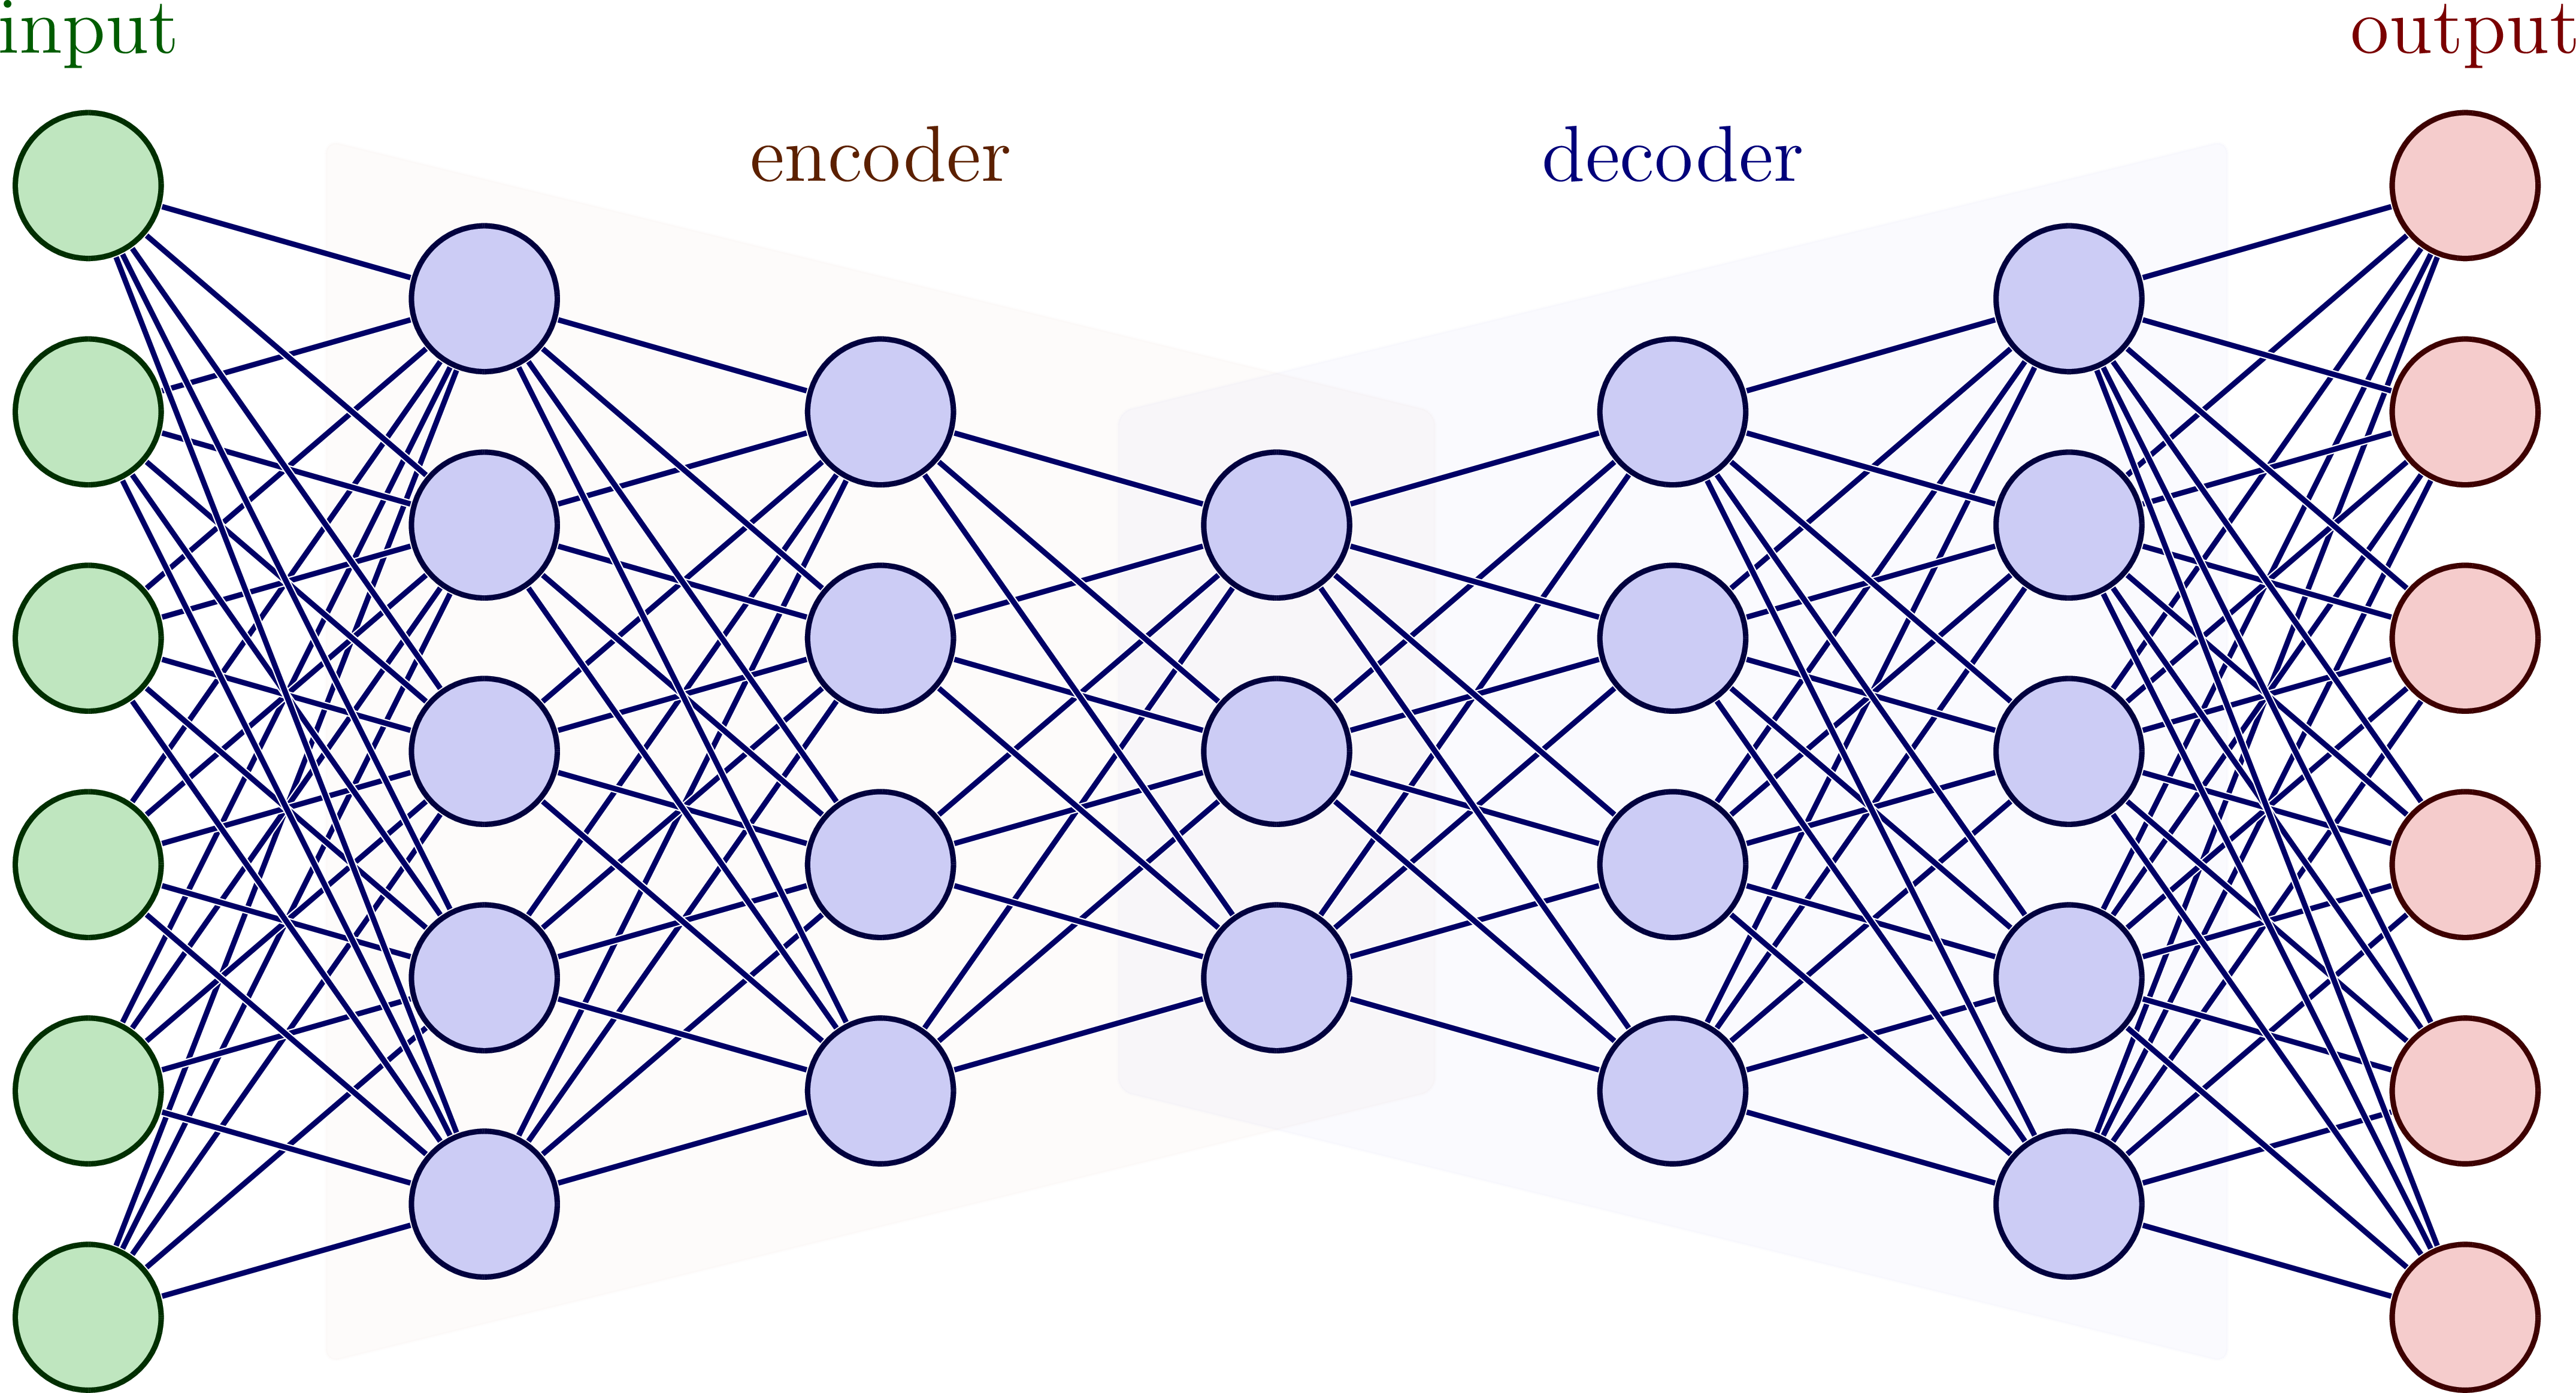
\includegraphics[width=0.9\linewidth]{images/encoder_decoder.png}
    \caption{Schéma du fonctionnement d'un encoder et d'un decodeur}
    \label{fig:encoder_decoder}
\end{figure}

Dans le Transformer, chaque bloc encodeur est constitué de plusieurs couches identiques empilées. Chacune de ces couches comprend : 
\begin{itemize} 
    \item une couche d’auto-attention multi-tête (self-attention) permettant à chaque token de la séquence d’entrée d’interagir avec les autres tokens, 
    \item un réseau feedforward positionnel appliqué de manière indépendante à chaque position, 
    \item des connexions résiduelles et une normalisation de couche (layer normalization) pour stabiliser et accélérer l’apprentissage. 
\end{itemize}

Le bloc décodeur repose sur une structure similaire, avec deux différences majeures : 
\begin{itemize} 
    \item une première couche de masked self-attention, empêchant chaque token de voir les tokens futurs (condition essentielle pour la génération auto-régressive), 
    \item une couche d’attention croisée (cross-attention) qui permet à chaque token généré de s’appuyer sur les représentations produites par l’encodeur.
\end{itemize}

Donc, le modèle Transformer complet, tel que présenté dans \citep{vaswani2017attention} ici en \autoref{fig:architecture_complete_transformers}, montre une visualisation détaillée de l’architecture complète d’un Transformer, avec empilement de couches identiques et passage des informations entre blocs encodeur et décodeur.

\begin{figure}[H]
    \centering
    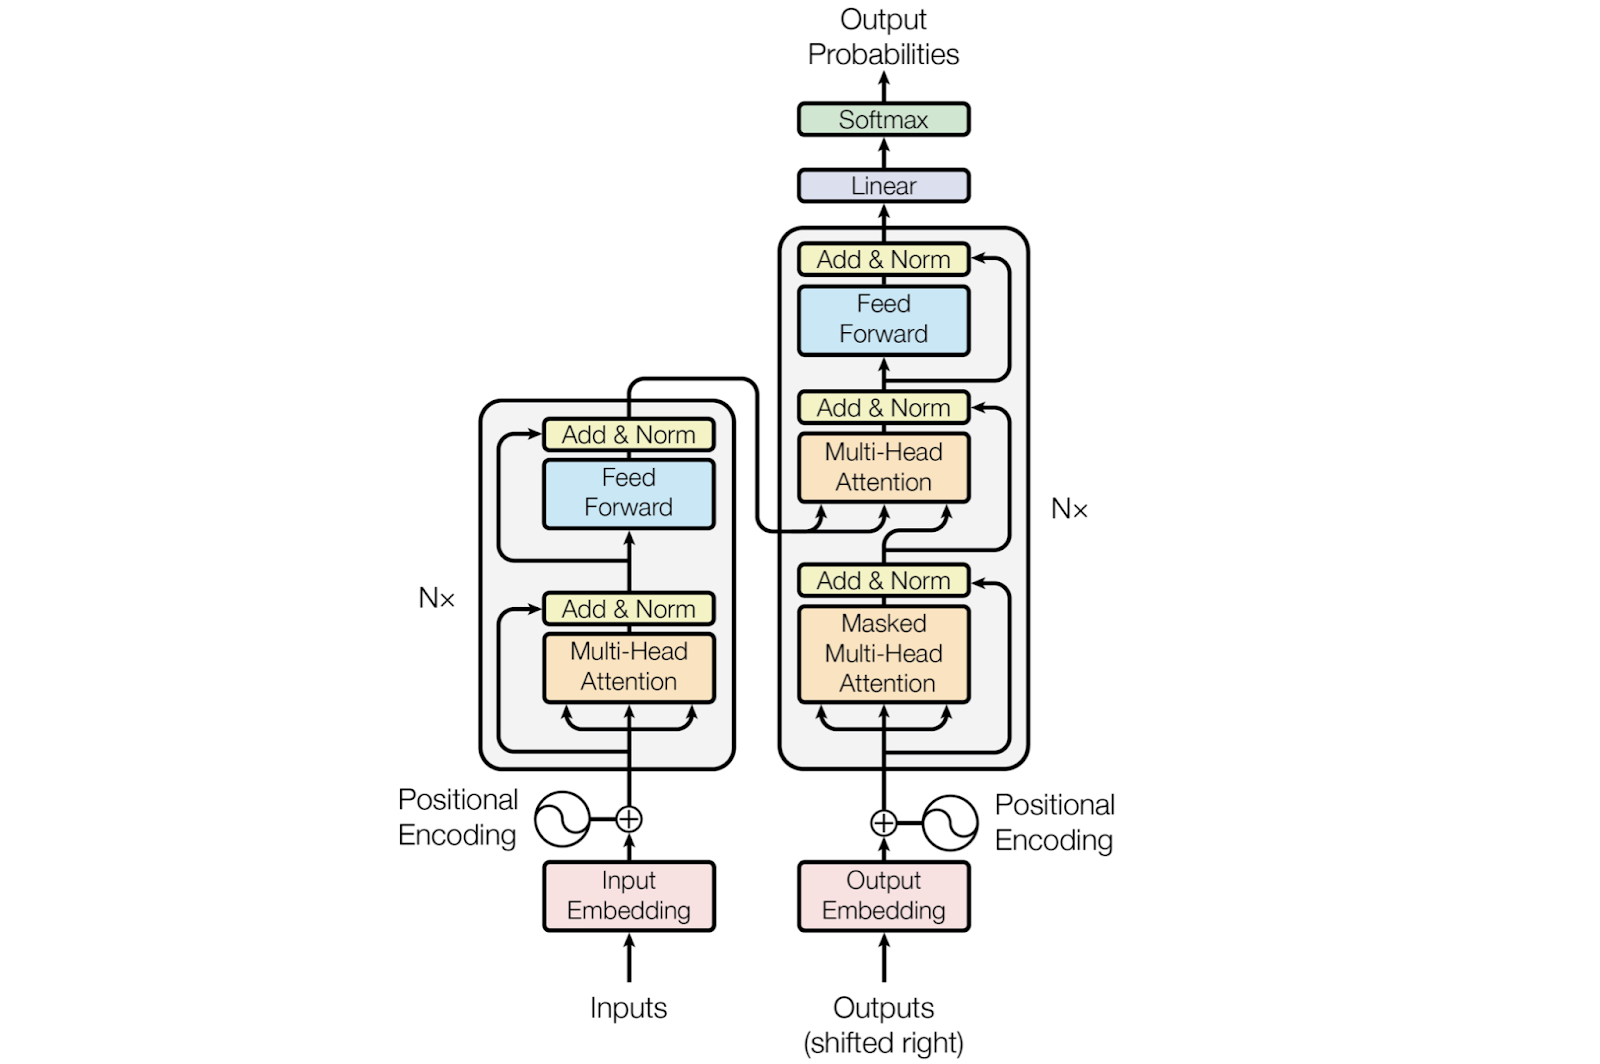
\includegraphics[scale=0.3]{images/transformers.png}
    \caption{Architecture complète du modèle transformers}
    \label{fig:architecture_complete_transformers}
\end{figure}

Selon les tâches visées, différentes variantes de cette architecture peuvent être utilisées. Par exemple, BERT repose uniquement sur la pile encodeur, ce qui le rend adapté aux tâches de classification ou d’extraction d’information. À l’inverse, les modèles comme GPT n’utilisent que la pile décodeur, car ils sont conçus pour la génération de texte. Enfin, les modèles T5 \citep{raffel2020t5} ou BART \citep{lewis2019bart} combinent encodeur et décodeur pour des tâches de traduction, de résumé ou de génération conditionnée.\\

En somme, l’architecture Transformer repose sur un agencement hiérarchique de mécanismes d’attention, complétés par des réseaux feedforward et des opérations de normalisation. Ce cadre modulaire, parallélisable et extensible a permis de dépasser les limites structurelles des réseaux récurrents, en particulier pour le traitement de longues séquences. L’utilisation conjointe de l’attention multi-tête, des encodages positionnels, et de blocs empilés confère au Transformer une capacité remarquable à modéliser les dépendances globales et locales dans les données séquentielles. Ce socle architectural a donné naissance à une large famille de modèles dérivés, chacun adapté à des tâches spécifiques. Parmi eux, BERT constitue une avancée importante en introduisant un pré-entraînement bidirectionnel basé sur cette architecture. 

\subsection{Encodage bidirectionnel profond}

L’efficacité des Transformers dans les tâches de traitement du langage repose essentiellement sur leur capacité à capter des dépendances de contexte à travers le mécanisme d’attention. Néanmoins, la structure modulaire de ces modèles permet des spécialisations architecturales adaptées aux besoins spécifiques des tâches : l’encodeur est utilisé pour extraire des représentations riches à partir d’un texte en entrée, tandis que le décodeur est employé pour la génération séquentielle. Parmi les approches exploitant uniquement la pile encodeur, le modèle BERT a introduit une innovation en adoptant un encodage bidirectionnel profond, permettant de tenir compte simultanément du contexte gauche et droit d’un mot. Ce paradigme bidirectionnel s’est avéré particulièrement performant pour les tâches de classification, de reconnaissance d'entités nommées ou encore de compréhension de texte. À travers ce paragraphe, seront analysés les fondements du modèle BERT, ses mécanismes de pré-entraînement multi-tâches (MLM et NSP), ainsi que ses variantes modernes comme ModernBERT, qui visent à étendre les performances et l'efficacité du modèle original en intégrant les dernières avancées en matière d'architecture et d’optimisation.

\subsubsection{BERT}

Le modèle \textbf{BERT} (\textit{Bidirectional Encoder Representations from Transformers}), introduit par \citep{devlin2018bert}, marque une avancée majeure dans le domaine du traitement automatique du langage naturel. Contrairement aux modèles précédents, comme ELMo \citep{peters2018deep} ou GPT \citep{radford2018gpt1}, BERT repose sur une approche bidirectionnelle de l'encodage, permettant au modèle de prendre en compte simultanément le contexte gauche et le contexte droit d’un mot à chaque couche de traitement.\\

Avant BERT, deux grandes stratégies dominaient le transfert d'apprentissage en NLP. L'approche \textit{feature-based}, représentée par ELMo, consistait à utiliser des représentations contextuelles pré-entraînées comme caractéristiques dans des architectures spécifiques à chaque tâche. D'autre part, l'approche \textit{fine-tuning}, popularisée par OpenAI GPT, consistait à pré-entraîner un modèle de langage unidirectionnel, puis à affiner tous ses paramètres sur une tâche cible.\\

BERT combine le meilleur des deux mondes avec une architecture unifiée qui peut être fine-tunée sur une grande variété de tâches sans modifications substantielles. Son architecture repose uniquement sur la pile encodeur du Transformer, sans composant de décodeur, ce qui convient parfaitement aux tâches de classification ou d'extraction. Deux versions principales ont été proposées :
\begin{itemize}
    \item \textbf{BERT\textsubscript{BASE}} : 12 couches (transformer blocks), dimension cachée $H=768$, 12 têtes d'attention, 110M paramètres.
    \item \textbf{BERT\textsubscript{LARGE}} : 24 couches, $H=1024$, 16 têtes, 340M paramètres.
\end{itemize}

Les performances de BERT ont établi de nouveaux records sur de nombreuses tâches, notamment le benchmark GLUE, SQuAD (question-réponse) et SWAG (inférence de bon sens). Son succès a rapidement engendré une série de variantes et d'améliorations, telles que RoBERTa, ALBERT ou encore DistilBERT.\\

L'apport de BERT s’explique en grande partie par une stratégie de pré-entraînement  reposant sur deux objectifs complémentaires : le Masked Language Modeling (MLM) et le Next Sentence Prediction (NSP). Ces mécanismes seront présentés dans ce qui suit.

\subsubsection{Méthode de pré-entraînement (Masked Language Model et Next Sentence Prediction)}

La phase de pré-entraînement de BERT repose sur deux objectifs principaux : le Masked Language Modeling (MLM) et la Next Sentence Prediction (NSP), qui permettent de doter le mod\`ele d'une représentation contextuelle bidirectionnelle profonde, adaptée à de nombreuses tâches en aval.\\

Le MLM, inspiré de la tâche de Cloze \citep{taylor1953cloze}, consiste à masquer de manière aléatoire une portion des tokens de la séquence d'entrée, et à prédire ces tokens à partir du contexte bidirectionnel fourni par les autres mots. Formellement, à partir d'une séquence $\mathbf{X} = (x_1, \dots, x_n)$, il est choisit 15\% des positions $\mathcal{M} \subset \{1, \dots, n\}$ à prédire. Pour chaque position $i \in \mathcal{M}$ :
\begin{itemize}
    \item 80\% du temps, est remplacé $x_i$ par le token [MASK],
    \item 10\% du temps, est remplacé $x_i$ par un mot aléatoire de l'espace lexical,
    \item 10\% du temps, est gardé $x_i$ inchangé.
\end{itemize}

Le mod\`ele apprend à prédire le mot d'origine $x_i$ à partir de l'encodage $T_i$ du token masqué via une softmax sur le vocabulaire $V$ :

\begin{equation}
\hat{x}_i = \operatorname*{argmax}_{v \in V} \; \mathrm{softmax}(T_i^\top E_v)
\end{equation}

o\`u $E_v$ est l'embedding du mot $v$. Cette méthode permet donc un apprentissage bidirectionnel à chaque couche du Transformer, contrairement aux modèles de langage traditionnels unidirectionnels. Toutefois, pour limiter l'écart entre l'entraînement et l'utilisation, le mot masqué n'est pas toujours remplacé par [MASK].\\

Le NSP, quant à lui, vise à apprendre des représentations de paires de phrases et à capturer les relations inter-phrastiques, essentielles pour des tâches comme l'inférence ou la réponse à une question.

À partir de deux phrases $A$ et $B$ extraites du corpus :
\begin{itemize}
    \item dans 50\% des cas, $B$ est bien la suite directe de $A$ (label : \texttt{IsNext}),
    \item dans 50\% des cas, $B$ est une phrase aléatoire du corpus (label : \texttt{NotNext}).
\end{itemize}

Le modèle apprend à prédire cette relation à partir du vecteur cachée $C$ associée au token [CLS] :

\begin{equation}
P(\text{IsNext}|A,B) = \mathrm{softmax}(\mathcal{W}^\top C + b)
\end{equation}
o\`u $W$ et $b$ sont les poids du classifieur NSP. BERT est pré-entraîné sur deux grands corpus non annotés : le \textit{BooksCorpus} (800M mots) et \textit{Wikipedia} anglais (2.5 milliards de mots), en extrayant uniquement les passages textuels.\\

L'apprentissage combine les deux objectifs avec une fonction de perte composée :

\begin{equation}
\mathcal{L} = \mathcal{L}_{\text{MLM}} + \mathcal{L}_{\text{NSP}}
\end{equation}

Les auteurs utilisent Adam avec warm-up et une décroissance linéaire du taux d'apprentissage, un dropout à 0.1 et une activation GELU \citep{hendrycks2016gaussian}. La \autoref{fig:pre-entrainement-bert} présente la séquence de pré-entraînement profond à gauche, multi-tâches et bidirectionnel  qui constitue l'apport de BERT vers une adaptation à des tâches spécifiques à droite sur une large variété de tâches NLP (c'est le fine tuning).

\begin{figure}[H]
    \centering
    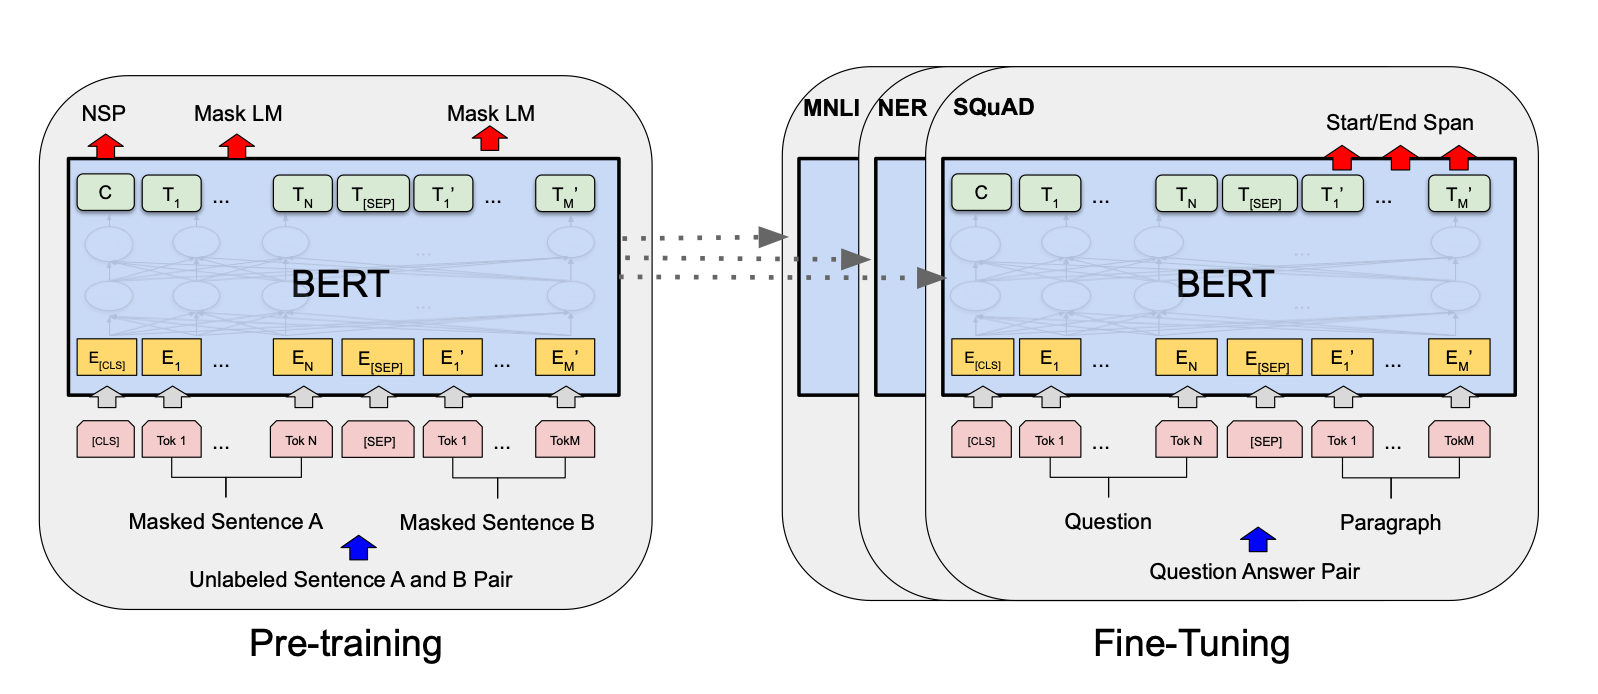
\includegraphics[scale=0.6]{images/BERT_entrainement.png}
    \caption{Méthode de pré-entraînement du modèle BERT}
    \label{fig:pre-entrainement-bert}
\end{figure}

Malgré ses avancées, BERT présente certaines limitations structurelles héritées de son époque, notamment en matière d’efficacité computationnelle, de capacité à traiter de longs contextes et d’utilisation d’architectures aujourd’hui considérées comme sous-optimales. Afin d’y remédier, plusieurs améliorations ont été proposées dans la littérature récente. Parmi elles, le modèle ModernBERT incarne une synthèse des meilleures pratiques actuelles par \citep{warner2024modernbert}.

\subsubsection{ModernBERT}

ModernBERT est un encodeur Transformer de nouvelle génération introduit par \citep{warner2024modernbert} pour remédier aux limitations connues de BERT, tout en intégrant les avancées modernes en architectures de modèles de langage. Conçu pour les usages discriminatifs (classification, retrieval, NLU), il constitue une optimisation de Pareto significative par rapport à BERT et ses dérivés, sur les axes de performance, d'efficacité mémoire et de vitesse d'inférence. Alors que les LLMs de type décodeur comme GPT dominent l'actualité, les encodeurs restent essentiels pour les tâches de compréhension de texte, de recherche d'information et de production de vecteurs denses utilisables dans des pipelines hybrides (RAG, réindexation, etc.). Or, ces tâches s'appuient encore largement sur BERT et RoBERTa \citep{liu2019roberta}, conçus entre 2018 et 2020. ModernBERT adopte une vision de rupture, fondée sur les outils matures de la génération moderne : RoPE, GeGLU, attention locale, etc.\\

Ce dernier possède des innovations architecturales principales :
\begin{itemize}
 \item Encodage positionnel Rotary (RoPE) : ModernBERT adopte l'encodage positionnel par rotation introduit dans RoFormer \citep{su2021roformer}. Plutôt que d'ajouter un vecteur de position comme dans BERT, RoPE applique une rotation aux vecteurs de requêtes et de clés en fonction de leur position. L'encodage positionnel est défini comme une rotation dans des sous-espaces 2D :

\begin{equation}
    f_{q,k}(x_i, i) = R_{\Theta, i} W_{q,k} x_i
\end{equation}

où $R_{\Theta, i} \in \mathbb{R}^{d \times d}$ est une matrice de rotation bloc-diagonale :

\begin{equation}
    R_{\Theta, i} = \text{diag}\left(
    \begin{bmatrix}
    \cos(i\theta_1) & -\sin(i\theta_1) \\
    \sin(i\theta_1) & \cos(i\theta_1)
    \end{bmatrix},
    \dots,
    \begin{bmatrix}
    \cos(i\theta_{d/2}) & -\sin(i\theta_{d/2}) \\
    \sin(i\theta_{d/2}) & \cos(i\theta_{d/2})
    \end{bmatrix}
    \right)
\end{equation}

avec :

\begin{equation}
    \theta_j = 10000^{-2(j-1)/d}
\end{equation}

Le produit scalaire entre une requête $q_m$ et une clé $k_n$ devient alors :

\begin{equation}
    q_m^\top k_n = (R_{\Theta,m} W_q x_m)^\top (R_{\Theta,n} W_k x_n)
    = x_m^\top W_q^\top R_{\Theta,m}^\top R_{\Theta,n} W_k x_n
\end{equation}

En définissant une matrice de rotation relative :

\begin{equation}
    R_{\Theta,n-m} := R_{\Theta,m}^\top R_{\Theta,n}
\end{equation}

il est obtenu l'expression finale du score d'attention :

\begin{equation}
    q_m^\top k_n = x_m^\top W_q^\top R_{\Theta,n-m} W_k x_n
\end{equation}

Cette formulation encode implicitement l'information de position relative entre tokens dans le score d'attention, tout en restant compatible avec les transformations linéaires habituelles du Transformer (\autoref{fig:rope_diagram}).

\begin{figure}[H]
    \centering
    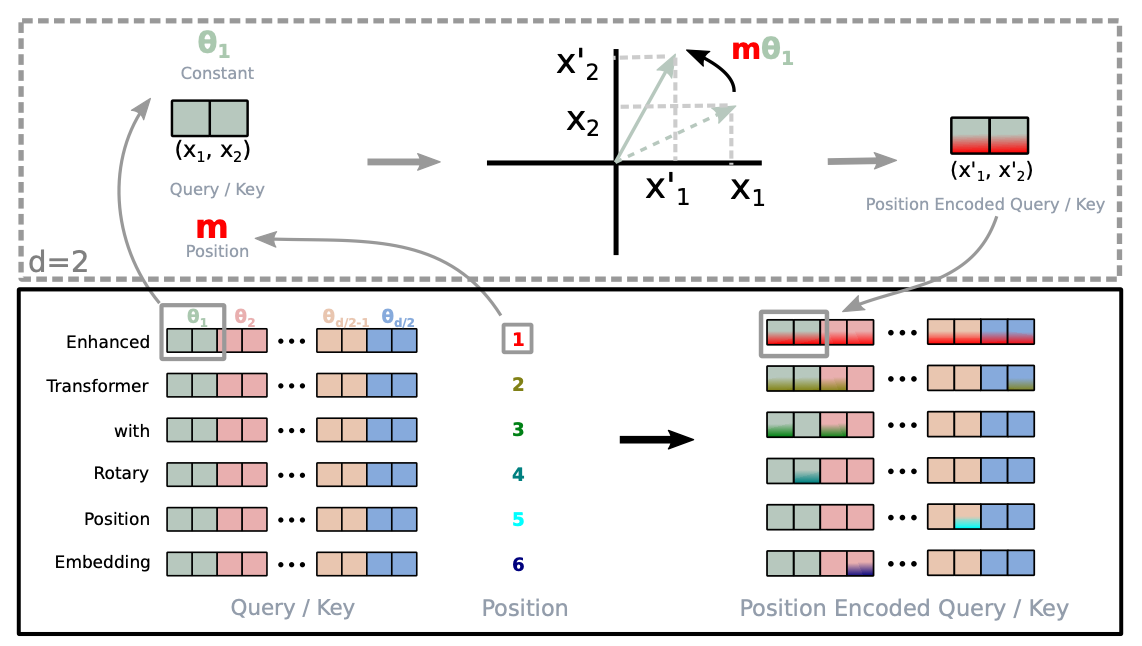
\includegraphics[width=0.9\linewidth]{images/ROPE.png}
    \caption{Implementation of Rotary Position Embedding (RoPE), adaptée de \citep{su2021roformer}}
    \label{fig:rope_diagram}
\end{figure}
    \item Normalisation pré-actuation (PreNorm) : chaque bloc Transformer sécrit comme :
    \[
    \mathbf{X}_{\text{out}} = \mathbf{X} + \text{FFN}(\text{LN}(\mathbf{X}))
    \]
    avec FFN une couche feed-forward et LN la normalisation couche.

    \item Activation GeGLU : la fonction non linéaire est remplacée par :
    \[
    \text{GeGLU}(x) = (x W_1) \odot \text{GELU}(x W_2)
    \]
    avec $W_1, W_2$ deux projections apprises tracées dans le plan (\autoref{fig:geglu_plot}).

    \begin{figure}[H]
    \centering
    \begin{tikzpicture}
        \begin{axis}[
            axis lines = middle,
            xlabel = $x$,
            ylabel = {GeGLU$(x)$},
            samples = 200,
            domain = -4:4,
            width=10cm,
            height=6cm,
            grid = major,
            thick,
            smooth,
            legend pos=south east,
        ]
            \addplot [blue] {x * 0.5 * (1 + tanh(sqrt(2/pi)*(x + 0.044715 * x^3)))};
        \end{axis}
    \end{tikzpicture}
    \caption{Représentation de la fonction GeGLU basée sur l’approximation de GELU}
    \label{fig:geglu_plot}
    \end{figure}

    \item Alternance d'attention globale et locale : les couches d'attention locale utilisent des fen\^etres de 128 tokens avec RoPE $\theta = 10{,}000$, les couches globales ont une rotation plus lente $\theta = 160{,}000$ pour capturer les dépendances longues. Plus précisément, les couches d'attention de ModernBERT sont organisées selon un motif où deux couches consécutives utilisent une attention locale, suivies d'une couche à attention globale. L'attention locale dans ces couches, chaque token n'assiste qu'à une fenêtre glissante centrée autour de lui. Par défaut, cette fenêtre est de taille 128 tokens. Concrètement, pour un token de position $i$, seuls les tokens $j$ tels que $|i - j| \leq 64$ sont pris en compte dans le calcul d'attention. Cela réduit la complexité de l'attention de $\mathcal{O}(n^2)$ à $\mathcal{O}(n w)$ où $w$ est la taille de la fenêtre (ici 128). Cette attention locale est enrichie par RoPE avec $\theta = 10{,}000$, adapté aux échelles courtes. Toutes les positions s'attendent mutuellement. Elle est appliquée toutes les trois couches, et utilise une version lente de RoPE ($\theta = 160{,}000$), permettant de capturer des dépendances sémantiques distantes.

    \item Unpadding complet : avant calcul de l'attention, les tokens de padding sont supprimés, réduisant la complexité effective du traitement.

    \item FlashAttention est une méthode d'implémentation de l'attention softmax qui permet un calcul exact en mémoire optimisée, exploitant la parallélisation matérielle des GPU modernes (Tensor Cores, CUDA pipelines). Contrairement à l'implémentation naïve qui calcule puis stocke toute la matrice $QK^\top$, FlashAttention découpe le calcul en blocs (\textit{tiling}) afin de minimiser les accès mémoire et d'éviter l'écriture de matrices intermédiaires en RAM. La version utilisée dans ModernBERT (FlashAttention-2 ou 3 selon le backend). Il permet une exactitude numérique garantie à une précision de $10^{-5}$ par calcul de softmax à somme compensée. Le calcul est fait directement pendant l'accumulation des blocs, réduisant la consommation mémoire à $\mathcal{O}(n d)$ au lieu de $\mathcal{O}(n^2)$ pour la matrice d'attention. Tri par longueur des séquences dans un batch, permettant un groupement efficace des tokens valides dans les buffers CUDA, ce qui améliore la coalescence mémoire. Aussi, il est compatible avec les optimisations comme l'	extit{unpadding}, le RoPE et l'attention locale/globale, ce qui le rend idéal pour des encodeurs long-contexte comme ModernBERT.
\end{itemize}

Le pré-entraînement de ce nouveau modèle repose uniquement sur le MLM, sans NSP, mais avec un taux de masquage à 30\%. Également, il y a une tokenisation BPE inspirée d'OLMo, avec 83 tokens spécifiques et une taille de vocabulaire de 50,368. L'Optimiseur StableAdamW avec warmup de 2\% et décroissance linéaire. Afin il y a un Packing dynamique des séquences pour maintenir un batch GPU dense et stable.\\

Deux configurations de modèles sont proposés dans le papier :
\begin{itemize}
    \item ModernBERT-base : 22 couches, 768 dimensions, 149M param\`etres
    \item ModernBERT-large : 28 couches, 1024 dimensions, 395M param\`etres
    \item Contexte maximal : 8192 tokens
\end{itemize}

\newpage

Les résultats empiriques en \autoref{fig:pareto-modernbert} démontrent l'optimisation de Pareto de ModernBERT : 

\begin{figure}[H]
    \centering
    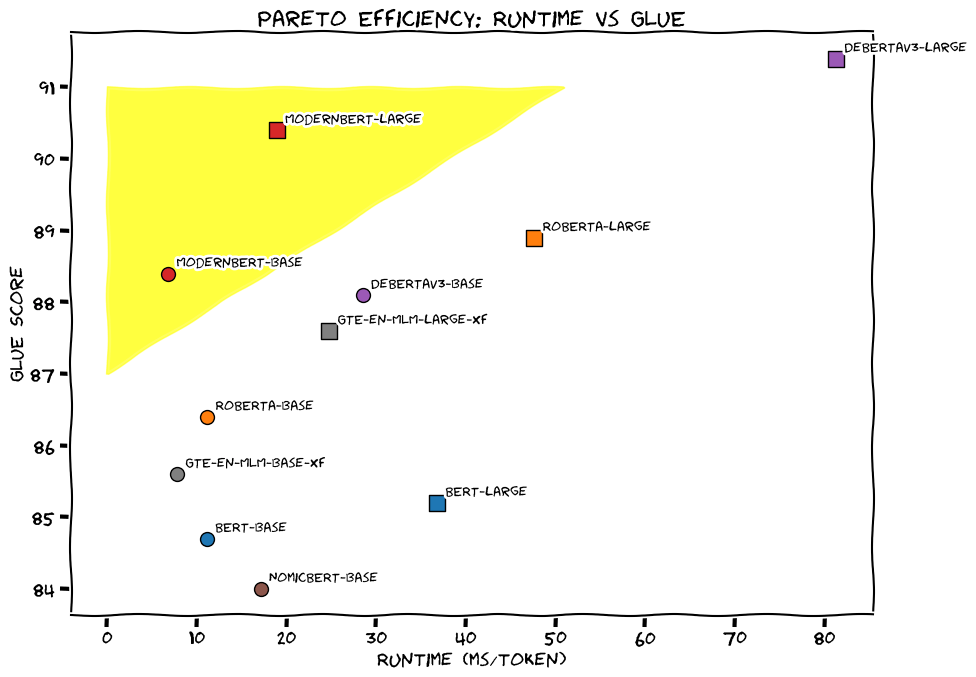
\includegraphics[width=0.9\linewidth]{images/modernbert_pareto_curve.png}
    \caption{Comparaison de l'efficience de Pareto Runtime vs GLUE}
    \label{fig:pareto-modernbert}
\end{figure}

Concernant les principales métriques de ModernBERT, le papier montre que pour GLUE benchmark surpasse DeBERTaV3-base tout en utilisant uniquement du MLM. Concernant BEIR / MLDR, il y a une meilleure précision en retrieval dense (BM25+encoder) et multi-vectoriel (ColBERT). Pour Code understanding, SOTA sur CodeSearchNet et StackQA, grâce à la présence de code dans le corpus de 2T tokens. Enfin, pour l'efficacité il y a jusqu'à 2$\times$ de rapidité que DeBERTaV3 pour des entrées longues. ModernBERT op\`ere asini une synth\`ese intelligente entre le paradigme LLM moderne et les besoins classiques de l'encodage, tout en conservant un design modulaire, open-source, et utilisable directement pour des cas d'usage industriels en retrieval, RAG ou classification.\\

L'architecture Transformer a fait évolué le champ du traitement automatique du langage, en remplaçant les mécanismes séquentiels classiques par une attention auto-référente efficace et massivement parallélisable. La première sous-section a détaillé les composants fondamentaux du modèle Transformer, en insistant sur le rôle  de la self-attention, des embeddings positionnels et du mécanisme multi-head, avant de présenter l’agencement général encodeur/décodeur. Ensuite, l’attention a été portée sur les architectures dérivées centrées sur l’encodage profond, avec en particulier BERT et ModernBERT, deux variantes qui illustrent l’évolution des modèles vers plus de profondeur. Toutefois, les Transformers présentent certaines limitations, notamment en ce qui concerne leur complexité quadratique en longueur de séquence, leur capacité à capturer des dépendances locales de manière efficace, ou encore leur intégration dans des systèmes contraints en ressources. Pour répondre à ces défis, de nouvelles architectures ont été proposées, mêlant modélisation continue, principes de l’espace d’état linéaire et efficience temporelle. L’une des plus prometteuses de cette nouvelle génération est l’architecture Mamba publié pour la première fois fin 2023.

\section{Architecture Mamba}

L’architecture Mamba s’inscrit dans une nouvelle génération de modèles séquentiels, conçus pour traiter efficacement des entrées de grande longueur tout en surmontant les limitations structurelles des architectures traditionnelles. Elle repose sur une intégration novatrice entre les mathématiques des \textit{State Space Models}, issus du contrôle et des systèmes dynamiques linéaires, et la flexibilité expressive des réseaux neuronaux profonds. En proposant une alternative aux Transformers, Mamba conserve une complexité temporelle linéaire,  tout en introduisant un mécanisme de sélection contextuelle, permettant une adaptation dynamique du modèle en fonction du contenu local des entrées pour la modélisation de longues séquences.\\

Les fondements théoriques de Mamba sont d'abord présentés, à travers une analyse des modèles linéaires à espace d’état, de leur formulation continue, puis de leur discrétisation numérique pour un usage efficace en contexte discret. Ensuite, l’introduction du mécanisme de sélection est détaillée. Ce mécanisme sera replacé dans le cadre plus large de l’architecture complète de Mamba, en lien avec les blocs MLP modernes et les réseaux récurrents. Mamba-2 est ensuite exposée. Ce dernier formalise une dualité structurée entre les SSMs et l’attention quadratique causale, permettant d’exploiter les deux modes de traitement dans un cadre unifié, plus efficace et plus parallèle. Enfin,  le modèle est présenté Llamba, une déclinaison récente et optimisée de Mamba-2, spécifiquement conçue pour la distillation depuis de grands modèles Transformers (tels que Llama-3). Llamba illustre l'application industrielle de Mamba dans des contextes contraints, tout en maintenant des performances grâce à une architecture légère et rapide à l’inférence.

\subsection{Fondements de Mamba}

La compréhension de l’architecture Mamba nécessite, avant, une étude des bases mathématiques sur lesquelles elle s’appuie. Contrairement aux modèles à attention, Mamba hérite directement de la théorie des systèmes dynamiques linéaires, en particulier des modèles à espace d’état, largement utilisés en contrôle automatique et traitement du signal. Ces modèles offrent une structure pour décrire l’évolution temporelle d’un système en fonction de ses entrées, à travers des équations différentielles ou des équations de récurrence discrètes. Ainsi, sont d’abord rappelés les principes théoriques des SSMs, leur formulation continue, ainsi que les principales méthodes de discrétisation permettant leur implémentation en environnement numérique. Ces éléments permettent à Mamba d'avoir ses propres innovations. En particulier, l’architecture repose sur l’idée que les dynamiques internes du système ne doivent plus être invariantes dans le temps, mais au contraire \textit{sélectivement adaptatives}, conditionnées par le contenu des séquences d’entrée. Cette perspective marque une rupture avec les SSMs classiques, et prépare la transition vers les mécanismes dynamiques spécifiques à Mamba détaillés dans les sous-sections suivantes.

\subsubsection{Contexte théorique : séquences longues et modèles linéaires structurés}

L'architecture Mamba, introduite en 2023 par \citep{gu2023mamba}, constitue une avance significative dans le domaine de la modélisation des séquences longues. Elle s'inscrit dans un effort de recherche visant à surmonter les limitations bien connues des Transformers en matière de complexité computationnelle et de capacité de généralisation sur des séquences de grande longueur.\\

Les Transformers, depuis leur introduction par \citep{vaswani2017attention}, ont dominé la modélisation de séquences dans une grande variété de domaines, allant du traitement du langage naturel à la génomique en passant par la vision par ordinateur. Leur capacité à capturer les dépendances globales grâce au mécanisme d'attention en a fait l'architecture de référence. Toutefois, ce mécanisme implique une complexité en temps et en mémoire quadratique en la longueur de la séquence, soit \( \mathcal{O}(L^2) \). Cela devient coûteux pour des entrées longues, telles que des documents complets, des séquences d'ADN, ou des flux audio continus.\\

Pour réduire cette complexité, plusieurs lignes de recherche ont émergé. Certaines se sont concentrées sur des variantes de l'attention, en tentant d'en rendre le coût sous-linéaire ou linéaire, comme dans Linformer, Performer, Longformer, ou Hyena \citep{poli2023hyena}. D'autres approches, plus radicales, ont proposé de s'affranchir totalement de l'attention pour revenir à des modèles récurrents ou convolutifs, tout en les modernisant grâce à une structuration mathématique inspirée de la physique et du contrôle : les State Space Models.\\

Les SSM structurés, popularisés par le modèle \textbf{S4} \citep{sun2023retnet}, offrent une alternative intéressante en modélisant une dynamique linéaire dans un espace latent, contrôlée par les entrées. Leur grande force réside dans leur complexité linéaire en la taille de la séquence, tout en permettant des calculs parallélisables via des convolutions efficaces. Ces modèles se sont montrés prometteurs sur des données audio, séquentielles continues, et génomiques.\\

Cependant, une limitation persistante des SSMs classiques est leur invariance temporelle : les paramètres gouvernant l'évolution de l'état latent (tels que les matrices de transition et les vecteurs d'entrée) sont fixes dans le temps. Cela rend ces modèles peu adaptatifs, notamment dans des contextes où l'information à mémoriser ou à ignorer varie en fonction du contenu. En d'autres termes, ils sont incapables de \textit{sélectionner dynamiquement} les informations pertinentes à conserver ou à oublier.\\

C'est cette limitation que Mamba cherche à lever. En introduisant le concept de Selective State Space Models, Mamba déforme le cadre traditionnel des SSMs pour permettre une dépendance explicite du contenu des entrées dans les dynamiques internes du modèle. Concrètement, les paramètres du modèle (tels que le vecteur de mise à jour de l'état ou le vecteur de sortie) deviennent eux-mêmes des fonctions non-linéaires des entrées. Cela permet une forme de sélection contextuelle, où le modèle apprend à filtrer, mettre en pause ou mettre à jour l'information en fonction du contenu local.\\

Ce changement de paradigme est profond : Mamba conserve les avantages d'efficacité des SSMs, mais acquiert la flexibilité fonctionnelle des architectures à attention. Pour y parvenir sans explosion de coûts mémoires, les auteurs conçoivent un algorithme de scan efficace sur GPU, qui simule le passage récursif à travers les états sans matérialiser l'ensemble de la trajectoire. Cette implémentation hautement optimisée permet à Mamba d'atteindre une vitesse d'inférence comparable à celle des RNNs tout en surpassant les Transformers sur plusieurs benchmarks, y compris sur des données textuelles, audio ou biologiques.\\

Cette première mise en contexte a permis de souligner les défis posés par les longues séquences ainsi que les limitations des architectures existantes, notamment l'invariance temporelle des modèles à espace d’état classiques. Pour mieux comprendre les fondements de Mamba et sa capacité à surmonter ces obstacles, il convient à présent de présenter les State Space Models avec leur formulation continue et discrète.

\subsubsection{State Space Models (SSM)}

Les modèles à espace d’état (State Space Models, ou SSM) constituent une classe puissante de modèles mathématiques largement utilisée dans les domaines du contrôle optimal, du traitement du signal et plus récemment de la modélisation de séquences longues. Leur formalisme repose sur la décomposition d’un système dynamique linéaire en deux équations fondamentales : une équation d’état et une équation d’observation.\\

La version continue d’un SSM linéaire temporellement invariant (LTI) est donnée par le système d’équations différentielles suivant :

\begin{equation}
\begin{cases}
\frac{d}{dt} h(t) = A h(t) + B u(t) \\
\quad y(t) = C h(t)
\end{cases}
\label{eq:ssm_continu}
\end{equation}

avec :
\begin{itemize}
    \item $h(t) \in \mathbb{R}^N$ : vecteur d'état caché à l'instant $t$,
    \item $u(t) \in \mathbb{R}^d$ : entrée externe (input),
    \item $y(t) \in \mathbb{R}^d$ : sortie observée,
    \item $A \in \mathbb{R}^{N \times N}$ : matrice de transition,
    \item $B \in \mathbb{R}^{N \times d}$ : matrice de contrôle,
    \item $C \in \mathbb{R}^{d \times N}$ : matrice d'observation.
\end{itemize}

Une méthode classique pour discrétiser le système continu \eqref{eq:ssm_continu} est le schéma d’intégration du trapèze, à mi-chemin entre les points $t$ et $t+1$. Elle est aussi connue comme la méthode bilinéaire ou Tustin. Il faut intégrer l’équation d’état sur l’intervalle $[t, t+\Delta]$ :

\begin{equation}
    h(t+\Delta) = h(t) + \int_t^{t+\Delta} \left( A h(s) + B u(s) \right) ds
\end{equation}

En appliquant la règle du trapèze, il est approximé l'intégrale par :
\begin{equation}
    h(t+\Delta) \approx h(t) + \frac{\Delta}{2} \left[ (A h(t) + B u(t)) + (A h(t+\Delta) + B u(t+\Delta)) \right]
\end{equation}

En regroupant les termes :
\begin{align*}
    h(t+\Delta) - \frac{\Delta}{2} A h(t+\Delta) &\approx h(t) + \frac{\Delta}{2} A h(t) + \frac{\Delta}{2} B \left( u(t) + u(t+\Delta) \right) \\
    \left( I - \frac{\Delta}{2} A \right) h(t+\Delta) &\approx \left( I + \frac{\Delta}{2} A \right) h(t) + \Delta B u_{\text{avg}}(t)
\end{align*}

avec $u_{\text{avg}}(t) = \frac{1}{2}(u(t) + u(t+\Delta))$. En posant :
\begin{equation}
\bar{A} = \left( I - \frac{\Delta}{2} A \right)^{-1} \left( I + \frac{\Delta}{2} A \right), \quad
\bar{B} = \left( I - \frac{\Delta}{2} A \right)^{-1} \Delta B
\end{equation}

ainsi la dynamique discrète :
\begin{equation}
    h_{t+1} = \bar{A} h_t + \bar{B} u_{\text{avg}}(t)
\end{equation}

Cette méthode garantit une bonne stabilité numérique, et est souvent utilisée dans les implémentations SSM modernes à cause de sa précision accrue par rapport à la méthode d’Euler explicite. La sortie observée reste :

\begin{equation}
    y_t = C h_t
\end{equation}

Cette récurrence peut s’écrire sous la forme d’une convolution. Pour cela, il suffit d’itérer les équations du système :

\begin{equation}
    x_k = \bar{A} x_{k-1} + \bar{B} u_k, \quad y_k = \bar{C} x_k
\end{equation}

Commençons par la première ligne du système :

étape 0 :
\begin{equation*}
    x_0 = \bar{B} u_0
\end{equation*}

étape 1 :
\begin{equation*}
    x_1 = \bar{A} x_0 + \bar{B} u_1 = \bar{A} \bar{B} u_0 + \bar{B} u_1
\end{equation*}

étape 2 :
\begin{equation*}
    x_2 = \bar{A} x_1 + \bar{B} u_2 = \bar{A}^2 \bar{B} u_0 + \bar{A} \bar{B} u_1 + \bar{B} u_2
\end{equation*}

Il est possible de constater que $x_k$ peut s’écrire comme une combinaison linéaire pondérée des entrées $u_0, \dots, u_k$ par des puissances successives de $\bar{A}$. Passant ensuite à la seconde ligne du système, où il est injecté les $x_k$ :

étape 0 :
\begin{equation*}
    y_0 = \bar{C} x_0 = \bar{C} \bar{B} u_0
\end{equation*}

étape 1 :
\begin{equation*}
    y_1 = \bar{C} x_1 = \bar{C} (\bar{A} \bar{B} u_0 + \bar{B} u_1) = \bar{C} \bar{A} \bar{B} u_0 + \bar{C} \bar{B} u_1
\end{equation*}

étape 2 :
\begin{equation*}
    y_2 = \bar{C} x_2 = \bar{C} (\bar{A}^2 \bar{B} u_0 + \bar{A} \bar{B} u_1 + \bar{B} u_2) = \bar{C} \bar{A}^2 \bar{B} u_0 + \bar{C} \bar{A} \bar{B} u_1 + \bar{C} \bar{B} u_2
\end{equation*}

Il est alors identifié un noyau de convolution discret :
\begin{equation}
    \bar{K}_k = (\bar{C}\bar{B}, \bar{C}\bar{A}\bar{B}, \dots, \bar{C}\bar{A}^k\bar{B})
\end{equation}

La sortie $y_k$ est donc donnée par :
\begin{equation}
    y_k = \sum_{\tau=0}^k \bar{K}_{k - \tau} u_{\tau} = (\bar{K} * u)_k
\end{equation}

Cette forme convolutionnelle est la base des implémentations rapides par transformée de Fourier (FFT) dans les SSMs modernes. Cette observation est essentielle pour l'implémentation efficace des SSMs : plut\^ot que de simuler les états $h_t$ un par un (récurrence lente), on peut calculer la sortie par convolution FFT avec le noyau $K$, ce qui permet un parallélisme GPU maximal.\\

Toutefois dans \citep{gu2021combining}, les auteurs démontrent que la méthode de discrétisation ZOH permet d'obtenir un meilleur résultat : 

\begin{equation}
    \frac{d}{dt} h(t) = A h(t) + B u(t), \quad y(t) = C h(t)
\end{equation}

Le but de la discrétisation par la méthode ZOH est d’obtenir une version discrète à pas fixe $\Delta$ de ce système. On suppose que l’entrée $u(t)$ est constante sur chaque intervalle $[k\Delta, (k+1)\Delta)$. La solution analytique de l'équation différentielle linéaire est :

\begin{equation}
    h(t + \Delta) = e^{A \Delta} h(t) + \int_0^\Delta e^{A (\Delta - \tau)} B u(t) \, d\tau
\end{equation}

Sous l’hypothèse ZOH ($u(t+\tau) = u(t)$ pour $\tau \in [0, \Delta]$), cela devient :

\begin{equation}
    h_{k+1} = e^{A \Delta} h_k + \left( \int_0^\Delta e^{A (\Delta - \tau)} \, d\tau \right) B u_k
\end{equation}
Or,
\begin{equation}
    \int_0^\Delta e^{A (\Delta - \tau)} d\tau = \left( \int_0^\Delta e^{A s} ds \right) = A^{-1} (e^{A \Delta} - I)
\end{equation}

(en supposant $A$ inversible).\\

D'où la forme discrète du système :
\begin{align}
    \bar{A} &= e^{A \Delta} \\
    \bar{B} &= (e^{A \Delta} - I) A^{-1} B \\
    \bar{C} &= C
\end{align}

La dynamique discrète est donc :
\begin{equation}
    h_{k+1} = \bar{A} h_k + \bar{B} u_k, \quad y_k = \bar{C} h_k
\end{equation}

Cette méthode a l’avantage de préserver la structure exponentielle de la solution du système, ce qui est utile dans les modèles comme S4 ou Mamba où les SSMs sont appliqués à des séquences temporelles longues.\\

Dans le cas d’un modèle à une dimension ($A = -\lambda$ scalaire, $B = 1$), il est obtenu : 
\begin{equation}
    \bar{A} = e^{-\lambda \Delta}, \quad \bar{B} = (1 - e^{-\lambda \Delta}) / \lambda
\end{equation}

Pour résumé il est obtenu avec les deux méthodes : 

\begin{table}[H]
\centering
\sffamily
\renewcommand{\arraystretch}{1.8}
\begin{tabular}{|c|c|c|}
\hline
\textbf{Discrétisation} & \textbf{Bilinéaire} & \textbf{ZOH} \\
\hline
\multirow{}{}{\textbf{Récurrence}} &
$\bar{A} = \left(I - \frac{\Delta}{2} A\right)^{-1}\left(I + \frac{\Delta}{2} A\right)$ &
$\bar{A} = e^{A\Delta}$ \\
& $\bar{B} = \left(I - \frac{\Delta}{2} A\right)^{-1} \Delta B$ &
$\bar{B} = (\bar{A} - I) A^{-1} B$ \\
& $\bar{C} = C$ & $\bar{C} = C$ \\
\hline
\textbf{Convolution} & $\bar{K}_k = (\bar{C}\bar{B}, \bar{C}\bar{A}\bar{B}, \dots, \bar{C}\bar{A}^k\bar{B})$ & $\bar{K} = \left( C e^{A\cdot k\Delta}(e^{A\Delta} - I)A^{-1}B \right)_{0 \leq k < L}$ \\
\hline
\end{tabular}
\caption{Discrétisation des équations d'état et expression du noyau de convolution}
\end{table}

Pour la ZOH, après avoir déroulé les calculs, on obtient en fin de compte :

\begin{equation}
    y_k = \sum_{j=0}^k \bar{C} \bar{A}^j \bar{B} u_{k-j} = \sum_{j=0}^k \bar{K}_j u_{k-j}
\end{equation}

Ce noyau peut \^etre précalculé ou appris de manière efficace, et est essentiel pour la parallélisation des calculs dans les SSMs modernes.\\

Dans le noyau de convolution développé plus haut, les coefficients $\bar{C}$ et $\bar{B}$ peuvent \^etre considérés comme des scalaires (ou vecteurs) apprenables. Concernant la matrice $\bar{A}$, il a été vu qu'elle intervient à la puissance $k$ au temps $k$, ce qui peut devenir co\^uteux en calcul pour des longues séquences. Une stratégie classique pour rendre les puissances de $\bar{A}$ faciles à calculer est de supposer que $\bar{A}$ est diagonale :

\begin{equation}
A = \begin{bmatrix}
\lambda_1 & 0 & \cdots & 0 \\
0 & \lambda_2 & \cdots & 0 \\
\vdots & \vdots & \ddots & \vdots \\
0 & 0 & \cdots & \lambda_n
\end{bmatrix} \Rightarrow A^k = \begin{bmatrix}
\lambda_1^k & 0 & \cdots & 0 \\
0 & \lambda_2^k & \cdots & 0 \\
\vdots & \vdots & \ddots & \vdots \\
0 & 0 & \cdots & \lambda_n^k
\end{bmatrix}
\end{equation}

Par le théorème spectral de l’algèbre linéaire, cela correspond à une classe de matrices dites normales. En pratique, le choix de la discrétisation (Euler, trapèze, etc.) et de l’initialisation de $\bar{A}$ joue un rôle crucial dans les performances du modèle. Il a été observé empiriquement que des matrices $A$ aléatoires donnent de très mauvais résultats, tandis qu’une initialisation issue de la matrice HiPPO (High-Order Polynomial Projection Operator) conduit à une nette amélioration (de 60 \% à 98\% de précision sur MNIST seq.).\\

La matrice HiPPO a été introduite dans \citep{gu2020hippo} puis reprise dans les modèles S4 \citep{sun2023retnet} et LSSL. Elle prend la forme suivante :

\begin{equation}
A_{nk} = \begin{cases}
(-1)^{n-k} (2k+1), & n > k \\
k + 1, & n = k \\
0, & n < k
\end{cases}
\end{equation}

Cette matrice n’est pas diagonale, ni même normale, mais elle peut être décomposée comme la somme d’une matrice normale et d’une matrice de rang faible, connue sous le nom de décomposition NPLR (Normal Plus Low Rank) :

\begin{equation}
A = V \Lambda V^{-1} + P Q^T
\end{equation}

La matrice $A$ peut être approchée par une matrice diagonalisable $A_0 = V \Lambda V^{-1}$, où $\Lambda$ est une matrice diagonale contenant les valeurs propres dominantes de $A$, et $V$ la base propre associée (approximative ou exacte). L’écart entre $A$ et $A_0$ est capturé par un terme $A - A_0 = P Q^T$, où $P$ et $Q$ sont de faible rang. Cela revient à dire que l’information non diagonalisable de $A$ est contenue dans une perturbation à faible rang. Ainsi, la structure $A = V \Lambda V^{-1} + P Q^T$ capture le comportement principal de $A$ via $\Lambda$ (facile à exponentier) et sa complexité contextuelle par $P Q^T$.\\

Les auteurs de S4 montrent que cette classe de matrices peut être exploitée efficacement par trois techniques algorithmiques : série génératrice tronquée, noyaux de Cauchy, et identité de Woodbury (cf. Algorithme 1 \autoref{fig:ssm-s4}). Les détails de la preuve montrant qu’une matrice NPLR peut être utilisée comme une matrice diagonale à coût efficace figurent dans les appendices B et C du papier \citep{sun2023retnet}. Dans une suite de travaux intitulée How to Train Your HiPPO \citep{gu2022trainhippo}, les auteurs ont affiné la manière de construire et d’initialiser la matrice HiPPO, donnant naissance à une version mise à jour du modèle connue sous les noms de S4 V2 ou S4 Updated, à opposer à S4 Original. Enfin, certains auteurs comme Ankit Gupta ont proposé d’utiliser directement une matrice diagonale apprise (plutôt qu’une structure NPLR), une approche aujourd’hui largement adoptée pour sa simplicité d’implémentation et ses bonnes performances pratiques.\\

Malgré leur efficacité, les SSMs LTI souffrent de plusieurs limitations. D’abord, l’invariance temporelle empêche l’adaptation dynamique aux entrées. Ensuite, le filtre convolutionnel $K$ est fixe pour toutes les entrées. Enfin, ils n’ont pas de mécanisme explicite de sélection contextuelle. C’est dans ce contexte que s’inscrit l’architecture Mamba, qui propose de lever ces limitations tout en conservant les avantages structurels des SSMs par un mécanisme de sélection.

\subsubsection{Mécanisme de sélection dans les SSMs}

Dans les modèles à espace d’état linéaire traditionnels, la dynamique est régie par des matrices fixes :
\begin{equation}
    h_t = \bar{A} h_{t-1} + \bar{B} x_t, \quad y_t = \bar{C} h_t
\end{equation}
Ces paramètres (\(\bar{A}, \bar{B}, \bar{C}\)) sont typiquement issus de la discrétisation d’un système linéaire continu, via une méthode comme le schéma bilinéaire ou ZOH, et restent invariants au cours du temps. Toutefois, un tel système ne peut pas s’adapter dynamiquement au contenu des entrées. Pour y remédier, le mécanisme de sélection introduit par Mamba permet de moduler dynamiquement le comportement du système à chaque pas de temps, en rendant le pas de temps \(\Delta_t\) dépendant de l’entrée \(x_t\).\\

Le mécanisme de sélection repose sur la modulation de la dynamique via un paramètre $\Delta_t$ appris conditionnellement à l’entrée :
\begin{equation}
    \Delta_t = \tau_\Delta (\text{Param} + s_\Delta(x_t))
\end{equation}
avec :
\begin{itemize}
    \item $\tau_\Delta$ : fonction d’activation positive et différentiable (par exemple softplus ou exp)
    \item $s_\Delta$ : projection linéaire (MLP ou Linear) de l’entrée $x_t$
\end{itemize}

Ce paramètre $\Delta_t$ est ensuite utilisé pour discrétiser le SSM de façon dynamique :
\begin{equation}
    \bar{A}_t, \bar{B}_t = \texttt{discretize}(\Delta_t, A, B)
\end{equation}

La récurrence devient alors :
\begin{equation}
    h_t = \bar{A}_t h_{t-1} + \bar{B}_t x_t, \quad y_t = \bar{C}_t h_t
\end{equation}

Le modèle peut choisir d’oublier ou de propager certaines entrées selon leur contenu. Il permet également de faire le lien entre les dynamiques discrètes récurrentes et continues. La sélection est continue et permet l’entraînement via gradient. Ce mécanisme est important dans l’architecture Mamba, où il est appliqué au niveau de la couche SSM pour permettre un traitement adaptatif et efficace des séquences longues.

\begin{figure}[H]
\centering
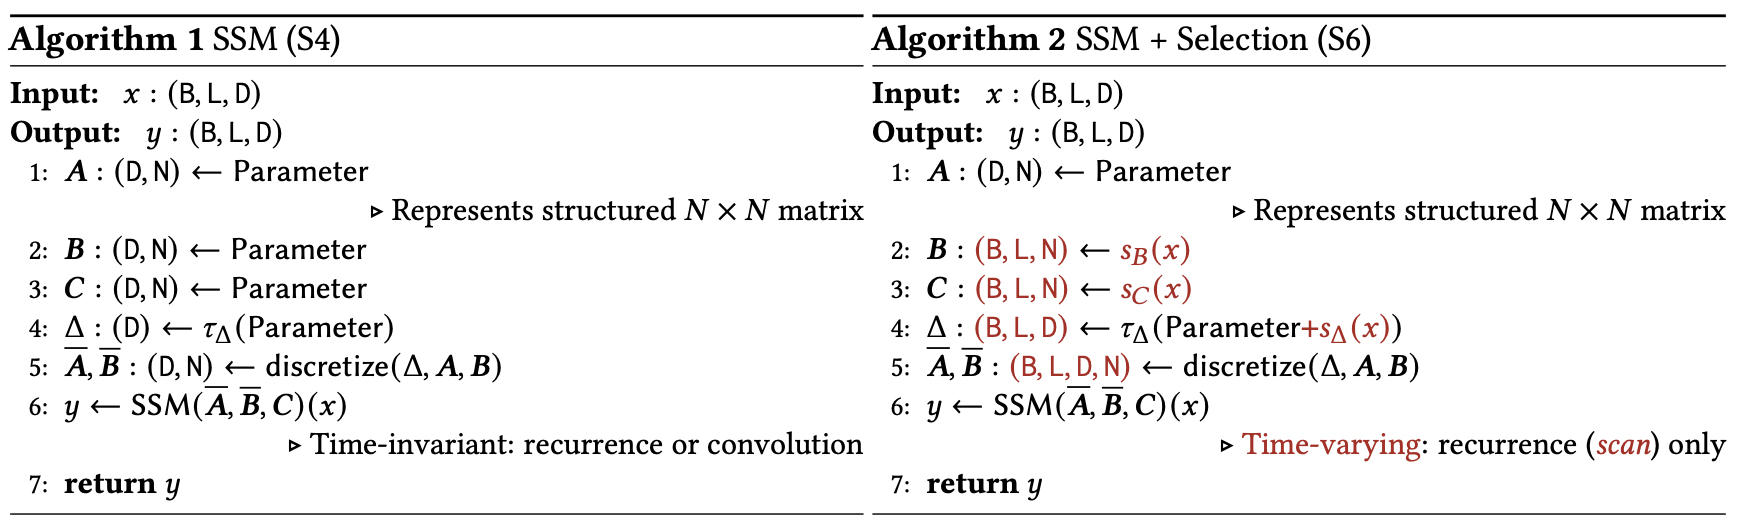
\includegraphics[scale=0.5]{images/algos_ssm_S4.png}
\caption{Algorithmes SSM S4 et SSM + Selection (S6)}
\label{fig:ssm-s4}
\end{figure}

La \autoref{fig:ssm-s4} compare l’implémentation classique (S4) avec celle enrichie du mécanisme de sélection (Mamba), en montrant l’évolution vers une dynamique dépendante du contenu, étape par étape.\\

Le mécanisme de sélection, en permettant de moduler dynamiquement les coefficients du modèle en fonction du contenu des entrées, constitue le cœur de l’innovation introduite par Mamba. Dans la section suivante, sera présentée l’architecture complète de Mamba, qui intègre ce mécanisme au sein d’un bloc modulaire, combinant efficacement transformations linéaires, non-linéarités, et traitement séquentiel parallèle. Cette architecture s’inscrit dans la continuité des RNNs modernes tout en introduisant des éléments conceptuellement proches des MLPs profonds.

\subsubsection{Architecture Mamba}

Le mécanisme de sélection introduit dans Mamba peut être interprété comme une généralisation des mécanismes de porte classiques des RNNs. Il a été observé que les portes des RNNs sont liées à la discrétisation de systèmes dynamiques en temps continu, une idée bien établie dans la littérature (voir \citep{funahashi1993approximation}, \citep{tallec2018can}). Dans cette optique, le paramètre $\Delta$ utilisé dans les SSMs s’interprète comme jouant un rôle généralisé des coefficients de porte des RNNs. Cette perspective permet d’établir un lien conceptuel entre les mécanismes heuristiques de porte et les fondations mathématiques rigoureuses des SSMs discrétisés. Ce lien est formalisé par le résultat au théorème 2.2.

\newpage

\begin{theorem}
Lorsque \( N = 1 \), \( A = -1 \), \( B = 1 \), \( s_{\Delta} = \text{Linear}(x) \), et \( \tau_{\Delta} = \text{softplus} \), alors la récurrence du SSM sélectif (Algorithme 2) devient :
\begin{align}
    g_t &= \sigma(\text{Linear}(x_t)) \\
    h_t &= (1 - g_t) h_{t-1} + g_t x_t
\end{align}
\end{theorem}

Il s’agit ici d’une amélioration du lemme 3.1 de \citep{gu2021combining}, généralisée à la discrétisation ZOH et aux portes dépendantes de l’entrée. La preuve complète est fournie dans l’annexe C de l’article original. Cette formulation met en évidence l’utilisation de $s_{\Delta}$ comme transformation linéaire de l’entrée, et de $\tau_{\Delta}$ comme activation de type softplus pour obtenir un coefficient $\Delta_t$ positif et différentiable. En particulier, lorsqu’une entrée $x_t$ doit être totalement ignorée — comme c’est le cas dans certaines tâches synthétiques — il est nécessaire que tous les canaux $D$ l’ignorent. Pour cela, il est proposé de projeter $x_t$ sur une dimension scalaire, puis de répéter cette valeur sur les $D$ canaux via une diffusion (broadcasting).\\

L’architecture d’un bloc Mamba peut s’interpréter comme une généralisation unifiée des blocs H3 et des MLPs à portes (Gated MLPs). Comme présenté en \autoref{fig:bloc-mamba}.

\begin{figure}[H]
    \centering
    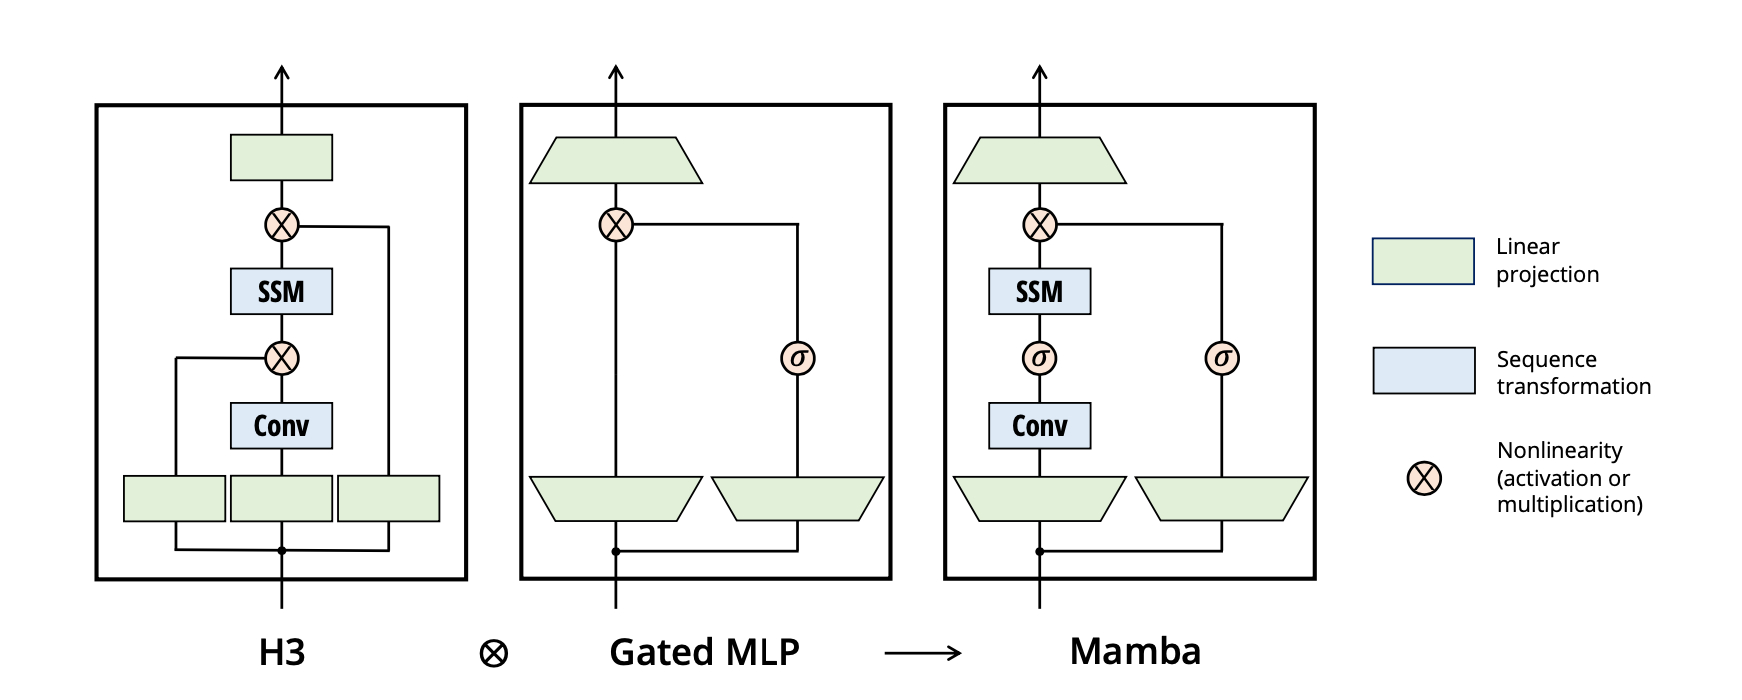
\includegraphics[width=1.0\linewidth]{images/mamba_architecture.png}
    \caption{\justifying Conception simplifiée de bloc combine le bloc H3 — qui constitue la base de la plupart des architectures à espace d’état — avec le bloc MLP, omniprésent dans les réseaux de neurones modernes. Au lieu d’alterner entre ces deux types de blocs, il est répété simplement le bloc Mamba de manière homogène. Par rapport au bloc H3, Mamba remplace la première porte multiplicative par une fonction d’activation. Par rapport au bloc MLP, Mamba ajoute un SSM (State Space Model) dans la branche principale. Pour la fonction d’activation $\sigma$, on utilise SiLU / Swish.}
    \label{fig:bloc-mamba}
\end{figure}

Elle intègre un SSM (State Space Model) comme transformation séquentielle principale, combiné à des projections linéaires et activations adaptatives. Premièrement, le Bloc H3 comporte deux branches parallèles (Conv et SSM), dont les sorties sont multipliées (gating). Ensuite, le Gated MLP structure purement MLP avec un produit entre une projection linéaire et une activation $\sigma$ de l’entrée (souvent SiLU). Pour finir, Mamba remplace le premier produit de H3 par une activation non-linéaire, et insère un SSM après une convolution. Le signal est donc filtré par la convolution, activé, puis intégré dynamiquement par le SSM. Le résultat est ensuite modulé par une autre activation. Le bloc Mamba applique donc les étapes suivantes :
\begin{enumerate}
    \item Deux projections linéaires en entrée (via Conv1D)
    \item Une branche passe dans un SSM (avec discrétisation adaptative)
    \item L’autre est activée via une fonction $\sigma$ (typiquement SiLU/Swish)
    \item Le produit à la sortie constitue l’output du bloc (gate multiplicatif)
\end{enumerate}

Ainsi, Mamba combine la structure hiérarchique (Conv + SSM) avec un mécanisme de sélection adaptatif (via $\Delta$) et la simplicité des blocs MLP modernes. Le tout forme un bloc homogène, empilé de manière répétée comme dans un Transformer. Contrairement à l’attention, le traitement est linéaire en la longueur de la séquence.\\

Mamba donc repose sur une refondation théorique des modèles à espace d’état linéaire, enrichis par un mécanisme de sélection contextuelle qui permet une adaptation dynamique aux entrées, tout en conservant une efficacité computationnelle linéaire. Cette architecture unifie plusieurs idées issues des réseaux de neurones modernes en les ancrant dans une modélisation continue et discrétisée de façon stable. Cette synthèse permis à Mamba de surpasser les Transformers sur plusieurs benchmarks séquentiels, tout en s'exécutant plus rapidement en inférence. Toutefois, malgré ses performances prometteuses, certaines limitations subsistent, notamment en termes de parallélisation des passes avant (forward pass) et de compatibilité avec les mécanismes d’attention traditionnels. C’est dans ce contexte qu’intervient Mamba-2, une extension  qui introduit une dualité structurée entre les modèles à espace d’état et l’attention quadratique, tout en renforçant la capacité de traitement parallèle. 

\subsection{Mamba-2}

Mamba-2 constitue une réponse directe aux limites de Mamba. Il propose un cadre unifié en articulant les SSMs autour d’une structure matricielle semi-séparable permettant une dualité explicite entre récurrence et attention. Cette reformulation ouvre la voie à un traitement parallèle plus rapide, tout en conservant les avantages structurels des SSMs. L’architecture est repensée pour faciliter la parallélisation des blocs, réduire les coûts d’inférence, et intégrer des schémas multi-têtes plus expressifs. Il est d'abord exposé les principales différences entre Mamba et Mamba-2, tant du point de vue algorithmique que de l’architecture du bloc élémentaire. Il est ensuite introduit le cadre théorique de la Structured State-Space Duality (SSD), qui établit une équivalence mathématique entre certains SSMs et des mécanismes d’attention quadratique structurée. L’exploitation algorithmique des matrices semi-séparables est démontré. Pour finir, l’architecture du bloc Mamba-2 est détaillée pour finir plusieurs optimisations systèmes sont analysées, conçues pour tirer parti du matériel moderne (multi-GPU).

\subsubsection{Différences et évolutions par rapport à Mamba}

La version Mamba-2 \citep{dao2024mamba2} constitue une amélioration théorique, algorithmique et systémique significative par rapport à la première version de Mamba \citep{gu2023mamba}. Alors que Mamba exploitait des State Space Models sélectifs avec des paramètres temporellement variables ($A_t, B_t, C_t$), Mamba-2 repose sur une version affinée de ces SSM sélectifs, tout en les intégrant dans un cadre dualisé plus riche, appelé Structured State-Space Duality (SSD).\\

Mamba-2 montre que certains SSMs structurés sont mathématiquement équivalents à une classe d’attention quadratique à masque structuré, au travers d'une matrice semi-séparable (semiseparable matrix). Cela permet de bénéficier à la fois de la forme récurrente linéaire (entraînement efficace) et de la forme quadratique (computation matricielle parallélisable). Simplification structurelle de $A$. Dans Mamba-2, la matrice $A_t$ de la récurrence est réduite à une identité multipliée par un scalaire, ce qui abaisse les coûts de pré-traitement et permet des calculs plus efficaces sur GPU/TPU. Utilisation de dimensions de tête $P$ plus grandes. Contrairement à Mamba où $P = 1$, Mamba-2 adopte des têtes multiples analogues à celles des Transformers (typiquement $P = 64$ ou $128$), facilitant l’usage de multiplications matricielles. Bloc parallélisable. Les projections linéaires dépendantes des données (par exemple $s_B(x)$) sont désormais placées en début de bloc, ce qui autorise une parallélisation tensorielle (comme dans Megatron). Intégration de structures analogues aux têtes d’attention. Mamba-2 introduit la notion de Grouped-Value Attention (GVA), une analogie des têtes multi-values (MVA) pour SSMs, permettant des variations d’architecture plus riches.\\

Empiriquement, Mamba-2 pareto-domine les Transformers++ et Mamba original à taille comparable sur les tâches de modélisation de langage. Par exemple, un modèle Mamba-2 avec 2.7B de paramètres entraîné sur 300B tokens dépasse les performances de Mamba 2.8B, Pythia 2.8B et même Pythia 6.9B sur The Pile. Les gains de temps d'entraînement sont aussi significatifs : jusqu’à 8 fois plus rapide que Mamba avec l’algorithme SSD. Enfin, les lois de scaling à la Chinchilla sont aussi vérifiées pour Mamba-2, renforçant son potentiel comme fondation pour des modèles de grande taille. Il est donc nécessaire de démontrer cette équivalence mathématique entre SSD et attention quadratique.

\subsubsection{Structured State-Space Duality (SSD) et attention quadratique}

L'un des apports théoriques majeurs de Mamba-2 est l'introduction du cadre de la Structured SSD, qui unifie les représentations récurrentes (type SSM) avec les mécanismes d'attention structurée.\\

Le point de départ est le système à espace d'état linéaire sélectif discretisé, de la forme :
\begin{equation}
    h_t = \bar{A}_t h_{t-1} + \bar{B}_t x_t, \quad y_t = \bar{C}_t h_t
\end{equation}

En développant cette récurrence\footnote{Pour simplifier les écritures, dans la suite toutes les matrices sont considérées comme discrétisées : $\bar{A} = A, \bar{B}=B, \bar{C}=C$.} dans le temps (\textit{unrolling}), on peut exprimer $h_t$ par :

\begin{equation}
\begin{split}
    h_t &= A_t h_{t-1} + B_t x_t \\
        &= A_t (A_{t-1} h_{t-2} + B_{t-1} x_{t-1}) + B_t x_t \\
        &= A_t A_{t-1} h_{t-2} + A_t B_{t-1} x_{t-1} + B_t x_t \\
        &= \dots \\
        &= \left(\prod_{i=s+1}^{t} A_i\right) B_s x_s + \dots + B_t x_t
\end{split}
\end{equation}

Ainsi, en injectant dans $y_t = C_t h_t$, on obtient :
\begin{align}
    y_t &= C_t h_t = C_t \left( \sum_{s=1}^{t} \left( \prod_{i=s+1}^{t} A_i \right) B_s x_s \right) = \sum_{s=1}^t K_{t,s} x_s
\end{align}

où le noyau $K \in \mathbb{R}^{L \times L}$ est appelé noyau convolutif ou matrice de transfert temporelle :
\begin{equation}
    K_{t,s} := C_t \left(\prod_{i=s+1}^{t} A_i\right) B_s
\end{equation}

Lorsque les matrices $A_t$ sont diagonales (ou m\^eme scalaires, c'est-à-dire $A_t = \lambda_t I$), les produits matriciels successifs deviennent scalaires (ou diagonaux), ce qui permet de factoriser les termes :
\begin{equation}
    \prod_{i=s+1}^t A_i = \exp\left(\sum_{i=s+1}^t \ln A_i\right)
\end{equation}
Dans le cas scalaire, on peut donc poser :
\begin{align*}
    U_t &= C_t \prod_{i=1}^t A_i \\
    V_s^\top &= \left(\prod_{j=1}^s A_j^{-1}\right) B_s
\end{align*}
ce qui donne :
\begin{equation}
    K_{t,s} = U_t V_s^T \quad \text{pour } s < t, \quad \text{et } 0 \text{ sinon}
\end{equation}

Ce type de matrice $K$ est appelé matrice semi-séparable causale, et se note $K = \text{tril}(UV^\top)$. Cette forme est mathématiquement équivalente à une attention causale quadratique sans normalisation (type Softmax), où $U_t$ joue le r\^ole de requ\^ete ($q_t$) et $V_s$ celui de clé ($k_s$) :
\begin{equation}
    y_t = \sum_{s < t} q_t^T k_s x_s
\end{equation}
avec $q_t = U_t$, $k_s = V_s$. La dualité SSD décrit ainsi un pont théorique entre la récurrence linéaire des SSMs (traitement à faible mémoire et en ligne) et les architectures attentionnelles (accès aléatoire à la séquence, traitement parallélisé).

\subsubsection{Matrices semi-separables et algorithme SSD}

Les bénéfices du développement du cadre théorique SSD entre les SSMs, l’attention et les matrices structurées résident dans l’utilisation de ces connexions pour améliorer à la fois les modèles et les algorithmes. Il est démontré que plusieurs algorithmes permettant de calculer efficacement les modèles SSD peuvent être dérivés d’algorithmes existants pour la multiplication de matrices structurées. Le résultat principal, sur le plan computationnel, est un algorithme capable de combiner les deux modes de traitement dans les modèles SSD : le mode linéaire (récursif) et le mode quadratique (attention). Cet algorithme est aussi efficace que les SSMs classiques en termes de coût computationnel (avec une complexité linéaire en la longueur de la séquence), tout en étant aussi adapté au matériel (hardware-friendly) que l’attention, en reposant essentiellement sur des multiplications matricielles.\\

\begin{definition}
Une matrice $M \in \mathbb{R}^{T \times T}$ est dite \textbf{N-semi-séparable} si toute sous-matrice strictement triangulaire inférieure a un rang au plus $N$.
\end{definition}

\begin{theorem}
Une matrice $M$ est N-SSS si elle peut s’écrire sous la forme :
\begin{equation}
    M_{ji} = C_j^\top A_{j} A_{j-1} \cdots A_{i+1} B_i \quad \text{pour } j \geq i
\end{equation}
avec $A_t \in \mathbb{R}^{N \times N}$, $B_t, C_t \in \mathbb{R}^{N}$.
\end{theorem}

Sous la forme globale, 
\begin{equation}
    y = Mx = \sum_{s=0}^t C_t^\top A_{t} A_{t-1} \cdots A_{s+1} B_s x_s
\end{equation}

\begin{definition}[Cas spécial 1-semi séparable]
Dans ce cas, $A_t$ devient un scalaire $a_t$, et la matrice $M$ est donnée par :
\begin{equation}
    M_{ji} = \prod_{k=i+1}^{j} a_k \quad \text{(cumprod)}
\end{equation}
\end{definition}

Il est possible de diviser la séquence en $B = T/Q$ chunks qui sont des blocs de taille $Q$.

\begin{equation}
M =
\begin{bmatrix}
M^{(0,0)} & 0        & 0        & \cdots & 0 \\
M^{(1,0)} & M^{(1,1)} & 0        & \cdots & 0 \\
M^{(2,0)} & M^{(2,1)} & M^{(2,2)} & \cdots & 0 \\
\vdots    & \vdots    & \vdots    & \ddots & \vdots \\
M^{(B-1,0)} & M^{(B-1,1)} & M^{(B-1,2)} & \cdots & M^{(B-1,B-1)}
\end{bmatrix}
\end{equation}

Dans le développement, le Bloc Diagonal (Local : Input $\rightarrow$ Output) :
\begin{equation}
    M^{(j,j)} = \text{SSM}(A_{jQ:(j+1)Q},\ B_{jQ:(j+1)Q},\ C_{jQ:(j+1)Q})
\end{equation}

Les blocs diagonaux sont simples à traiter, car ils correspondent à des sous-problèmes auto-similaires de taille plus petite. Le bloc $j$-ième correspond au calcul de la sortie :
\[ 
\text{SSM}(A_R, B_R, C_R)(x_R)
\]
pour l'intervalle $R = jQ : (j + 1)Q = (jQ, jQ + 1, \ldots, jQ + Q - 1)$.\\


L'élément clé est que ce bloc peut être calculé avec n'importe quelle méthode souhaitée. En particulier, pour de petites tailles de chunk $Q$, ce sous-problème est plus efficacement résolu en utilisant la forme quadratique duale SMA. De plus, les chunks peuvent être calculés en parallèle. Ces sous-problèmes peuvent être interprétés comme : « quelle est la sortie par chunk en supposant que l'état initial (du chunk) est nul ». Autrement dit, pour le chunk $j$, il est calculé les sorties correctes en ne tenant compte que des entrées locales $x_{jQ : (j + 1)Q}$.\\

Le Bloc Hors-Diagonale (Low Rank : Inter-chunk) :
\begin{equation}
    M^{(j,i)} =
    \left[
    \begin{array}{c}
        C_{jQ}^\top A_{jQ:(i+1)Q-1} \\
        \vdots \\
        C_{(j+1)Q - 1}^\top A_{(j+1)Q - 1:(i+1)Q - 1}
    \end{array}
    \right]
    \cdot
    \left[
    \begin{array}{c}
        B_{iQ}^\top A_{iQ+1:(i+1)Q -1} \\
        \vdots \\
        B_{(i+1)Q - 1}^\top
    \end{array}
    \right]^\top
\end{equation}

Chaque bloc est de rang \( \leq N \). Par exemple, \autoref{fig:exemple_blocs}, pour \( T = 9 \) avec une décomposition en chunks de longueur \( Q = 3 \). Les cellules ombrées représentent les factorisations de rang faible des blocs hors-diagonaux de la matrice semi-séparable.

\begin{figure}[H]
    \centering
    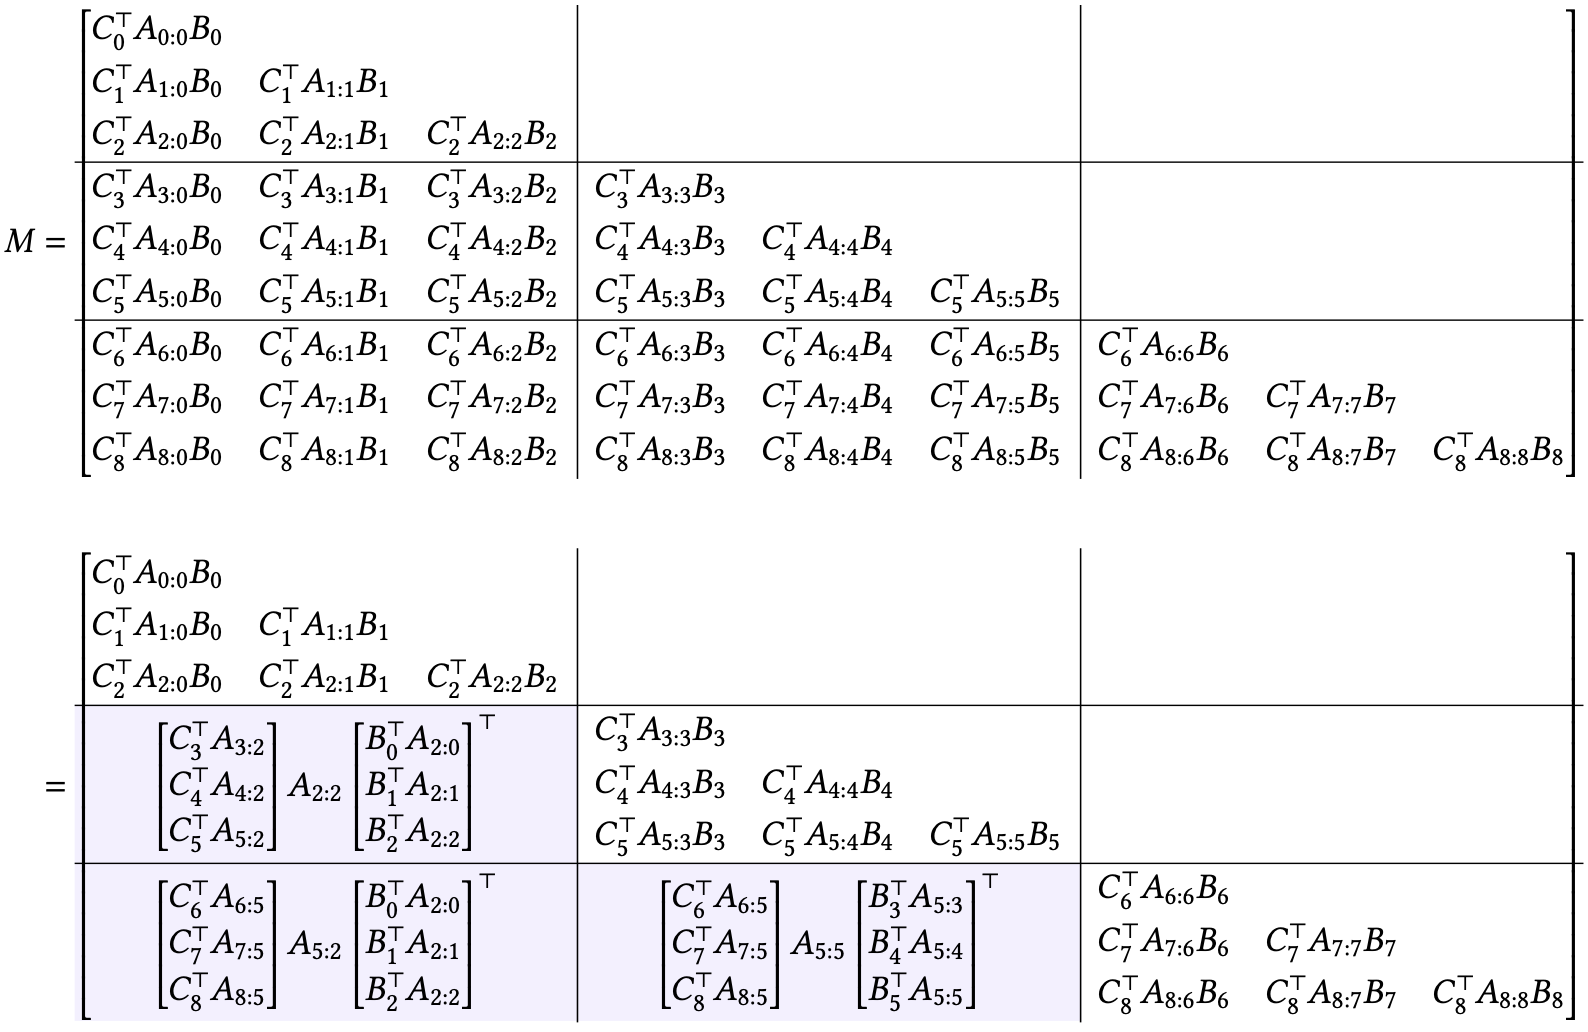
\includegraphics[width=1.0\linewidth]{images/matrices_semi_separables.png}
    \caption{\( T = 9 \) avec une décomposition en chunks de longueur \( Q = 3 \)}
    \label{fig:exemple_blocs}
\end{figure}

Il est possible à partir de cette structure de décomposer le problème en deux parties. Cela revient à diviser la sortie d’un chunk \( y_{jQ:(j+1)Q} \) en deux composantes :  
\begin{itemize}
    \item l’effet des entrées dans le chunk, soit \( x_{jQ:(j+1)Q} \) ;
    \item l’effet des entrées précédentes au chunk, soit \( x_{0:jQ} \).
\end{itemize}

La factorisation de rang faible consiste en trois termes, et il y a donc trois composantes distinctes dans le calcul associé. Dans cette factorisation, on utilise la terminologie suivante :

\begin{itemize}
    \item Les termes de la forme :
    \[
    \begin{bmatrix}
    B_0^\top A_{2:0} \\
    B_1^\top A_{2:1} \\
    B_2^\top A_{2:2}
    \end{bmatrix}
    \]
    sont appelés les facteurs droits ou blocs-$B$ (\emph{right factors} ou \emph{$B$-block-factors}). Cette étape consiste à effectuer la multiplication par les blocs-$B$ (facteurs droits) de la factorisation de rang faible. Pour chaque chunk, il s'agit d'une multiplication de matrice de taille $(N, Q)$ par $(Q, P)$, où $N$ est la dimension de l’état caché et $P$ est la dimension de la tête. Le résultat est un tenseur de dimension $(N, P)$ pour chaque chunk, ce qui correspond à l’état caché $h$ à l’issue du chunk. Cela peut s’interpréter comme : \og quel est l’état final produit par un chunk si l’on suppose que l’état initial de ce chunk est nul \fg. En d’autres termes, cela calcule $h_{jQ+Q-1}$ en supposant que $x_{0:jQ} = 0$.

    \item Les termes comme $A_{5:2}$ sont appelés les facteurs centraux ou blocs-$A$ (\emph{center factors} ou \emph{$A$-block-factors}). Cette étape calcule l’effet des blocs-$A$ (facteurs centraux) dans la factorisation de rang faible. À l’étape précédente, les états finaux de chaque chunk ont une forme globale de dimension $(T/Q, N, P)$. Ils sont multipliés maintenant par une matrice 1-SS construite à partir de :
    \[
    A_{2Q-1:Q-1},\ A_{3Q-1:2-Q-1},\ \dots,\ A_{T-1:T-Q-1}
    \]
    Cette étape peut être réalisée avec n’importe quel algorithme de multiplication de matrice 1-SS (à savoir, l’opérateur scan scalaire SSM ou \emph{cumprodsum}).
    \item Les termes de la forme :
    \[
    \begin{bmatrix}
    C_6^\top A_{6:5} \\
    C_7^\top A_{7:5} \\
    C_8^\top A_{8:5}
    \end{bmatrix}
    \]
    sont appelés les facteurs gauches ou blocs-$C$ (\emph{left factors} ou \emph{$C$-block-factors}). Cette étape réalise la multiplication par les blocs-$C$ (facteurs gauches) dans la factorisation de rang faible. Pour chaque chunk, cette opération peut \^etre vue comme une contraction matricielle de type $\text{contract}(QN, NP \rightarrow QP)$. On peut l'interpréter comme suit : \og quelle est la sortie par chunk si l'on dispose du bon état initial $h_{jQ-1}$ et que les entrées locales $x_{jQ:(j+1)Q}$ sont nulles \fg. En d'autres termes, pour le chunk $j$, cela permet de calculer les sorties correctes en ne tenant compte que des entrées précédentes $x_{0:jQ}$.
\end{itemize}

\begin{figure}[H]
    \centering
    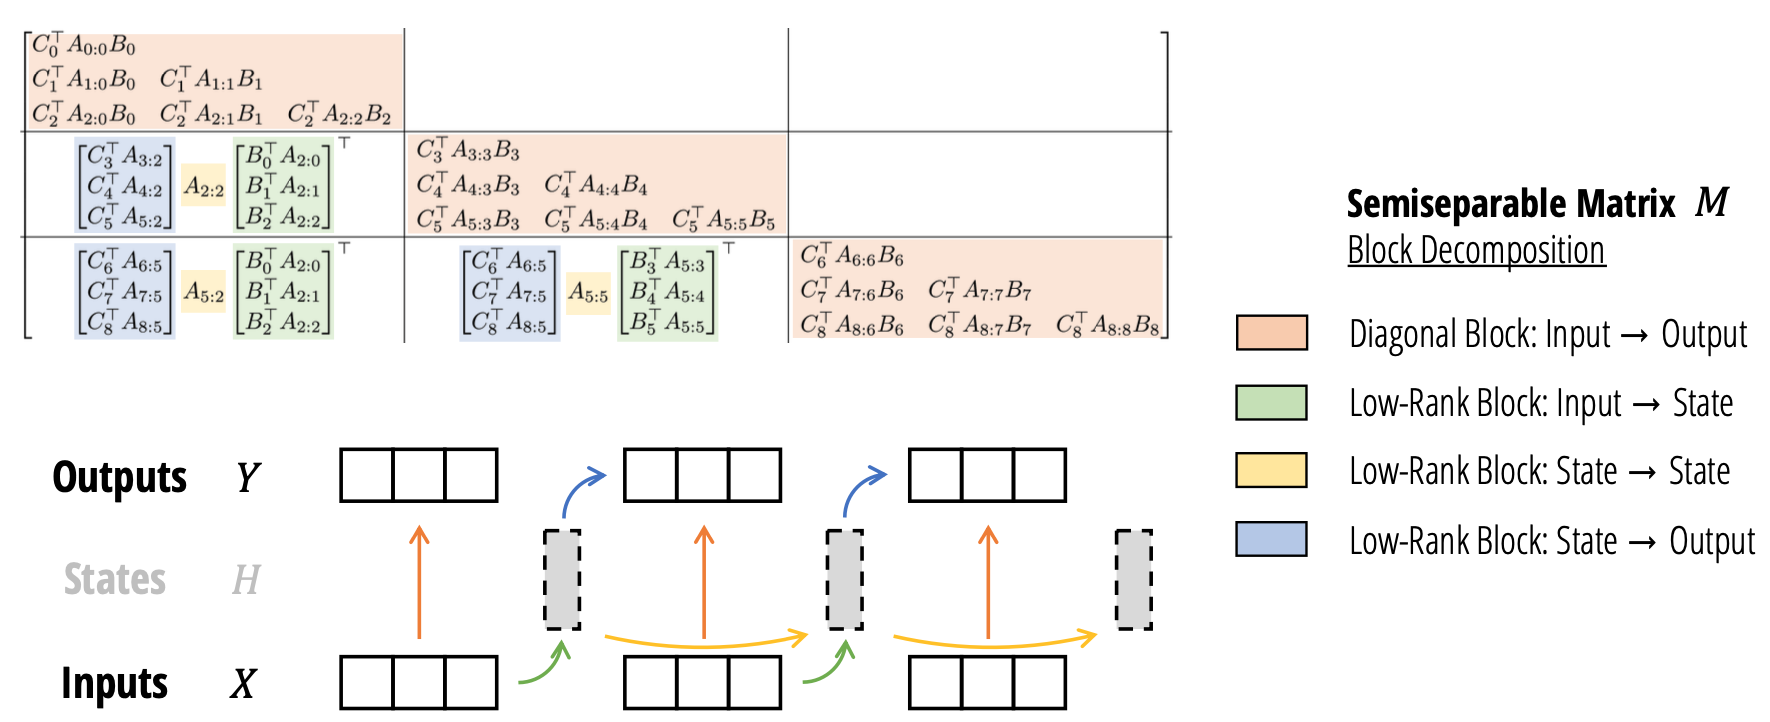
\includegraphics[width=1.0\linewidth]{images/sdd_algorithm.png}
    \caption{\justifying \textbf{(Algorithme SSD.)} En utilisant le point de vue transformation matricielle des modèles à espace d'état pour les réécrire sous forme de matrices semi-séparables, il est développé un calcul plus efficace matériellement du modèle SSD à travers un algorithme de multiplication matricielle par décomposition en blocs \citep{dao2024mamba2}.}
    \label{fig:ssd_algo}
\end{figure}

Cette multiplication matricielle présénté par l'algorithme SSD en \autoref{fig:ssd_algo} admet aussi une interprétation comme un modèle à espace d'état, où les blocs correspondent au découpage de la séquence d'entrée et de sortie en chunks. Les blocs diagonaux représentent les calculs intra-chunk, tandis que les blocs hors-diagonaux représentent les calculs inter-chunks, transmis via l'état caché du SSM. Concrètement, l'algorithme SSD décompose l'action du noyau convolutionnel temporel $K \in \mathbb{R}^{T \times T}$ en blocs diagonaux (intra-chunk) et hors-diagonaux (inter-chunk), où les blocs inter-chunks sont approximés par des produits de matrices de rang faible. Cette décomposition exploite la représentation semi-séparable des modèles SSM, pour lesquels la sortie $y_t$ peut s’écrire comme une somme pondérée des entrées passées selon la formule :

\begin{equation}
y_t = \sum_{s=1}^t K_{t,s} x_s = \sum_{s=1}^t C_t \left( \prod_{i=s+1}^{t} A_i \right) B_s x_s
\end{equation}

où les poids $K_{t,s}$ correspondent à une convolution causale générée par la dynamique linéaire du système. L’idée centrale de SSD est donc de transcrire cette relation récurrente en une forme matricielle factorisable, c’est-à-dire :

\begin{equation}
K = \mathrm{tril}(UV^\top)
\end{equation}

avec $\displaystyle U_t = C_t \prod_{i=1}^t A_i$ et $V_s^\top = \displaystyle \left( \prod_{j=1}^s A_j^{-1} \right) B_s$, ce qui correspond à une factorisation de rang faible causale.\\

L’algorithme SSD exploite donc cette factorisation en divisant la séquence en blocs temporels, puis en distinguant en les calculs locaux (intra-chunk), résolus via des SSM classiques sur une fenêtre glissante. Mais aussi par des les interactions longue portée (inter-chunk), traitées efficacement grâce à une factorisation de rang faible des contributions passées, via les matrices blocs-$A$, blocs-$B$, blocs-$C$.\\

Après avoir exposé le cadre théorique sous-jacent à l'algorithme SSD et sa mise en œuvre à travers les matrices semi-séparables, il est désormais possible d'en comprendre l'intégration concrète dans l'architecture Mamba-2, en particulier à travers la conception de ses blocs computationnels et les choix de factorisation mis en œuvre pour optimiser l'inférence et l'entraînement.

\subsubsection{Architecture Mamba-2}

Le bloc Mamba-2 est défini comme une simplification de l'architecture Mamba initiale. Les projections linéaires séquentielles y sont supprimées, ce qui réduit la complexité computationnelle. 

\begin{figure}[H]
    \centering
    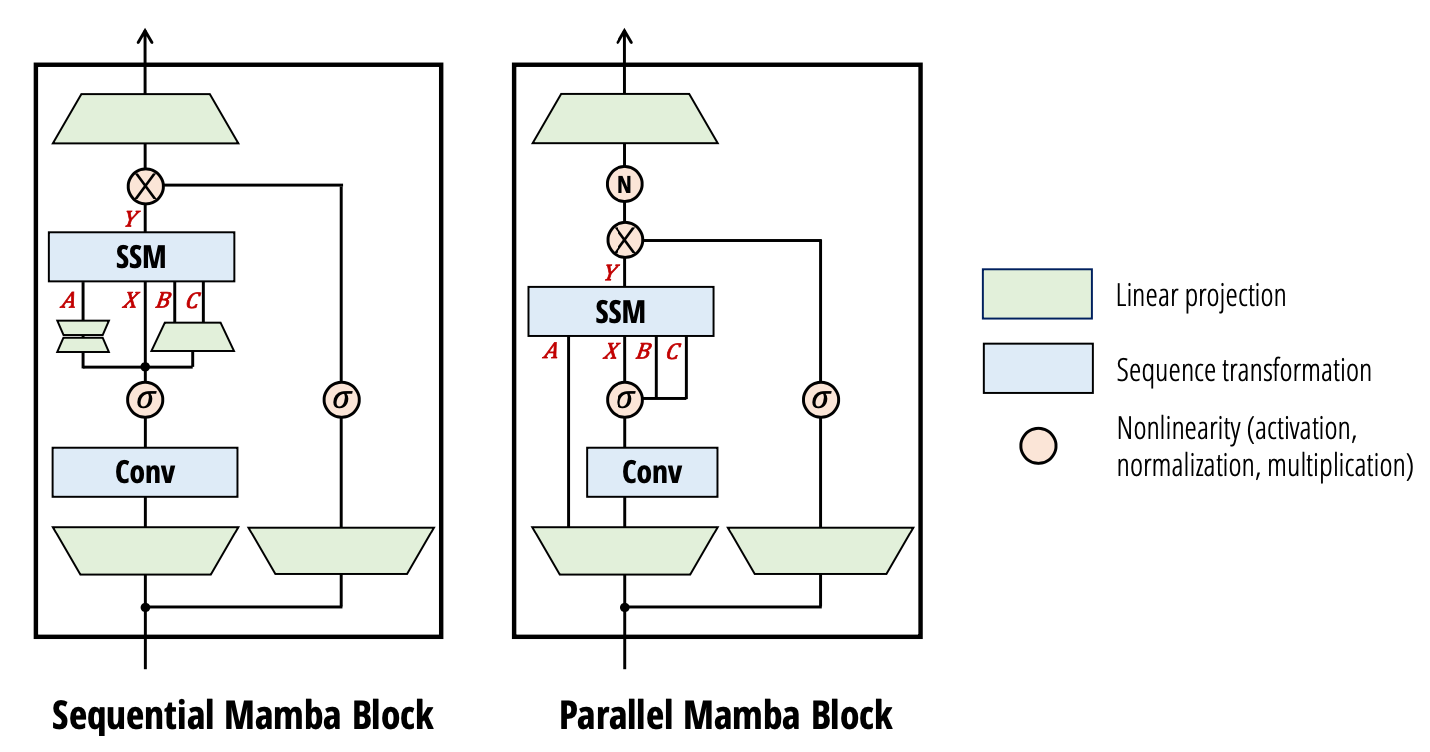
\includegraphics[width=1\linewidth]{images/mamba-2_architecture.png}
    \caption{\justifying Les paramètres du SSM \( A, B, C \) sont directement générés en début de bloc, plutôt qu'en fonction de l'entrée \( X \), ce qui permet une parallélisation plus efficace et une réduction des délais d'inférence. De plus, une couche de normalisation supplémentaire, inspirée de NormFormer \cite{shleifer2021normformer}, est ajoutée pour améliorer la stabilité de l'entraînement. Enfin, les projections $B$ et $C$ utilisent une seule tête partagée entre les différentes têtes $\mathbf{X}$, de manière analogue à l'attention multi-valeurs (Multi-Value Attention, MVA) \citep{dao2024mamba2}.}
    \label{fig:enter-label}
\end{figure}

\paragraph{Projections de paramètres parallèles.} Dans Mamba-1, une vision centrée sur les SSM était adoptée, dans laquelle la couche SSM sélective était considérée comme une application $\mathbf{X} \mapsto Y$. Les paramètres SSM $A, B, C$ étaient alors considérés comme secondaires et définis comme des fonctions de l’entrée $\mathbf{X}$. Ainsi, les projections linéaires définissant $(A, B, C)$ étaient appliquées \emph{après} la projection linéaire initiale produisant $\mathbf{X}$.\\

Dans Mamba-2, la couche SSD est considérée comme une application $(A, X, B, C) \mapsto Y$. Il est donc jugé logique que $A, X, B, C$ soient produits en parallèle, à l’aide d’une seule projection au début du bloc. Cette approche est analogue aux architectures d’attention classiques, où $\mathbf{X}, B, C$ correspondent respectivement aux projections $Q, K, V$ qui sont générées simultanément.\\

L’adoption des projections parallèles pour les entrées $A, B, C, X$ du SSM permet une réduction modérée du nombre de paramètres, mais surtout, elle rend le modèle plus compatible avec le parallélisme tensoriel, en particulier dans le cadre de modèles de grande taille, selon les schémas de partitionnement proposés dans Megatron \citep{shoeybi2019megatron}.

\paragraph{Normalisation supplémentaire.}Lors d’expériences préliminaires, des instabilités ont été constatées dans les grands modèles. Ces instabilités ont pu être atténuées par l’ajout d’une couche de normalisation supplémentaire (comme LayerNorm, GroupNorm ou RMSNorm) juste avant la projection de sortie finale du bloc.\\

L’usage de cette normalisation s’inspire directement de l’architecture NormFormer \citep{shleifer2021normformer}, où des couches de normalisation sont également ajoutées à la fin des blocs MLP et MHA.\\

Il est également noté que cette modification est similaire à celles introduites dans d’autres modèles récents proches de Mamba-2, conçus selon une perspective d’attention linéaire. Dans les formulations d’attention linéaire d’origine, une normalisation est effectuée par un terme au dénominateur simulant celle de la fonction softmax utilisée dans l’attention classique. Les modèles TransNormerLLM \citep{qin2023transnormerllm} et RetNet \citep{sun2023retnet} ont montré que cette forme de normalisation pouvait induire de l’instabilité, ce qui a motivé l’ajout d’une couche LayerNorm ou GroupNorm supplémentaire après la couche d’attention linéaire.\\

La couche de normalisation supplémentaire proposée ici diffère légèrement : elle est placée après la branche de porte multiplicative (multiplicative gate), et non avant.

\paragraph{Schémas multi-têtes pour les transformations de séquence.} En rappelant  que les SSMs sont définis comme des transformations de séquence dans lesquelles :
\begin{itemize}
    \item les paramètres $A, B, C$ ont une dimension d'état $N$ ;
    \item ils définissent une transformation de séquence $\mathbb{R}^T \rightarrow \mathbb{R}^T$, qui peut par exemple être représentée par une matrice $M \in \mathbb{R}^{T \times T}$ ;
    \item cette transformation opère sur une séquence d'entrée $\mathbf{X} \in \mathbb{R}^{T \times P}$, indépendamment sur l'axe $P$.
\end{itemize}

\newpage

Cela peut être interprété comme la définition d'une seule tête de transformation de séquence.

\begin{definition}[Schémas multi-têtes] Une transformation de séquence multi-têtes est composée de $H$ têtes indépendantes, pour un modèle de dimension totale $D = d \cdot H$. Les paramètres peuvent être partagés entre les têtes, ce qui définit un schéma de têtes.
\end{definition}

La taille d'état $N$ et la dimension de tête $P$ sont respectivement analogues à la dimension des têtes $QK$ et à celle des têtes $V$ dans l'attention. De même que dans les architectures Transformer modernes \citep{chowdhery2023palm, touvron2023llama}, dans Mamba-2, ces dimensions sont généralement choisies comme des constantes (typiquement 64 ou 128). Lorsque la dimension du modèle $D$ augmente, le nombre de têtes est augmenté, tout en gardant les dimensions $N$ et $P$ constantes. Pour décrire cette stratégie, les idées issues de l'attention multi-têtes peuvent être transférées et généralisées afin de définir des schémas similaires pour les SSMs ou toute autre transformation de séquence générale :
\begin{itemize}
    \item MHS (Multihead SSM) : chaque tête est une copie indépendante du SSM avec ses propres paramètres $A, B, C$. Le nombre de têtes est $H = D / P$. Ce schéma est analogue à l'attention multi-têtes classique (MHA), mais généralisable à toute transformation de séquence.
    \item MCS (Multi-contract SSM) : les paramètres $B$ et $\mathbf{X}$ (analogues à $V$ et $K$ dans l'attention) sont partagés entre les têtes, tandis que $C$ est spécifique à chaque tête. Cela rappelle le schéma de l'attention multi-queries (MQA), connu pour accélérer l'inférence autoregressive \citep{shazeer2019multiquery}.
    \item MES (Multi-expand SSM) : $C$ et $\mathbf{X}$ sont partagés entre les têtes, mais $B$ est indépendant, ce qui permet une expansion différente des états cachés pour chaque tête (analogue à multi-key attention).
    \item MIS (Multi-input SSM) : ici, $\mathbf{X}$ est vu comme l’entrée principale du SSM, et $B$, $C$ sont partagés à travers tous les canaux. Ce schéma, appelé aussi MVA (multi-value attention), correspond à l’architecture de Mamba originale, où chaque canal d’entrée a sa propre dynamique $A$ mais partage les paramètres $B, C$.
\end{itemize}

\newpage

\begin{proposition} La couche SSM sélective (S6) dans l’architecture Mamba \citep{gu2023mamba} peut être interprétée ainsi comme une dimension de tête $P = 1$ : chaque canal possède une dynamique SSM indépendante définie par $A$. Lastructure de tête MIS (ou MVA) : les matrices $B$ et $C$ (équivalentes à $K$ et $Q$ dans l’attention) sont partagées entre tous les canaux d’entrée $\mathbf{X}$ (analogue à $V$).
\end{proposition}

Ces variantes de schémas de tête peuvent être ablatées dans les SSD. Malgré un contrôle strict du nombre de paramètres et de la dimension d’état totale, des différences notables de performance sont observées en aval. Il a été empiriquement constaté que le schéma MVA utilisé dans Mamba donne les meilleurs résultats.\\

Au-delà des innovations architecturales, les performances de Mamba-2 reposent également sur une série d’optimisations système pensées pour l'entraînement et l'inférence à grande échelle. Ces optimisations exploitent pleinement les caractéristiques des matrices semi-séparables, tout en assurant une compatibilité maximale avec les schémas de parallélisme modernes.

\subsubsection{Optimisation pour Mamba-2}

Il est ainsi présenté plusieurs optimisations système pour les modèles à espace d’état, en particulier dans l’architecture Mamba-2, afin d’assurer un entraînement et une inférence efficaces à grande échelle.

\paragraph{Parallélisme tensoriel}

Le parallélisme tensoriel est une technique de parallélisation du modèle qui consiste à décomposer chaque couche (comme l’attention ou les MLPs) pour les faire fonctionner sur plusieurs dispositifs (ex : GPUs). Cette approche est largement utilisée pour entraîner des modèles de grande taille \citep{shoeybi2019megatron, brown2020gpt3, chowdhery2023palm, touvron2023llama}.

\newpage

Dans Mamba-1, soit une entrée $u \in \mathbb{R}^{L \times d}$ (pas de batching pour simplifier), les projections linéaires s’effectuent comme suit :
\begin{align*}
    x &= u \mathcal{W}^{(x)\top} \in \mathbb{R}^{L \times ed} \\
    z &= u \mathcal{W}^{(z)\top} \in \mathbb{R}^{L \times ed} \\
    x_c &= \text{conv1d}(x) \in \mathbb{R}^{L \times ed} \\
    (\Delta, B, C) &= \text{projection faible rang}(x_c) \\
    y &= \text{SSM}_{A,B,C,\Delta}(x_c) \in \mathbb{R}^{L \times ed} \\
    y_g &= y \cdot \phi(z) \quad \text{(gating, avec $\phi$ = SiLU)} \\
    \text{out} &= y_g \mathcal{W}^{(o)\top} \in \mathbb{R}^{L \times d}
\end{align*}

Toutefois, lorsque l’on tente de décomposer $\mathcal{W}^{(x)}$ et $\mathcal{W}^{(z)}$ sur deux GPUs, il faut faire un \textit{all-reduce} entre les GPUs pour récupérer $x_c$ avant de pouvoir projeter $(\Delta, B, C)$. Cette synchronisation ajoute une communication supplémentaire par rapport à l’attention classique (qui n’en nécessite qu’une seule).\\

C’est pourquoi avec Mamba-2, pour n’avoir qu’un seul \textit{all-reduce} par bloc (comme dans les Transformers), Mamba-2 définit $(\Delta, B, C)$ directement depuis $u$ au lieu de $x_c$. Cela permet de paralléliser les projections dès le début.

\begin{align*}
    x^{(i)} &= u \mathcal{W}^{(x)\top} \in \mathbb{R}^{L \times ed} \\
    z^{(i)} &= u \mathcal{W}^{(z)\top} \in \mathbb{R}^{L \times ed} \\
    (\Delta^{(i)}, B^{(i)}, C^{(i)}) &= \text{projection}(u) \quad \text{(par GPU)} \\
    x^{(i)}_c &= \text{conv1d}(x^{(i)}) \in \mathbb{R}^{L \times ed} \\
    y^{(i)} &= \text{SSM}_{A,B,C,\Delta}(x_c^{(i)}) \in \mathbb{R}^{L \times ed} \\
    y^{(i)}_g &= y^{(i)} \cdot \phi(z^{(i)}) \\
    y^{(i)}_n &= \text{GroupNorm}(y_g^{(i)}) \quad \text{(nombre de groupes divisible par degré TP)} \\
    \text{out}^{(i)} &= y_n^{(i)} \mathcal{W}^{(o)\top} \in \mathbb{R}^{L \times d}
\end{align*}

Ainsi, les matrices de projection $\mathcal{W}^{(x)}, \mathcal{W}^{(z)}, \mathcal{W}^{(o)}$ peuvent être décomposées. Aussi, un seul \textit{all-reduce} est requis en fin de bloc de fait chaque GPU contient un sous-ensemble de $(\Delta, B, C)$ ("groupes logiques").\\

Formalisme pour 2 GPUs : pour un degré de TP = 2, il est décomposé :
\begin{align*}
    \mathcal{W}^{(x)} &= [\mathcal{W}^{(x)}_1, \mathcal{W}^{(x)}_2], \quad \mathcal{W}^{(x)}_i \in \mathbb{R}^{d \times ed/2} \\
    \mathcal{W}^{(z)} &= [\mathcal{W}^{(z)}_1, \mathcal{W}^{(z)}_2], \quad \mathcal{W}^{(z)}_i \in \mathbb{R}^{d \times ed/2} \\
    \mathcal{W}^{(o)} &= \begin{bmatrix} \mathcal{W}^{(o)}_1 \\ \mathcal{W}^{(o)}_2 \end{bmatrix}, \quad \mathcal{W}^{(o)}_i \in \mathbb{R}^{ed/2 \times d}
\end{align*}

Chaque GPU effectue alors le traitement sur sa propre partition $x^{(i)}, z^{(i)}$, produit $y^{(i)}$, applique $\phi$, la normalisation, puis produit $\text{out}^{(i)}$. Finalement, un \textit{all-reduce} est appliqué :

\[
\text{out} = \sum_i \text{out}^{(i)}
\]

Grâce à cette architecture \autoref{fig:mamba2_gpu}, Mamba-2 rend le parallélisme tensoriel aussi efficace que celui de l’attention ou des MLP dans les Transformers. L’utilisation de GroupNorm évite les synchronisations intermédiaires.

\begin{figure}[H]
    \centering
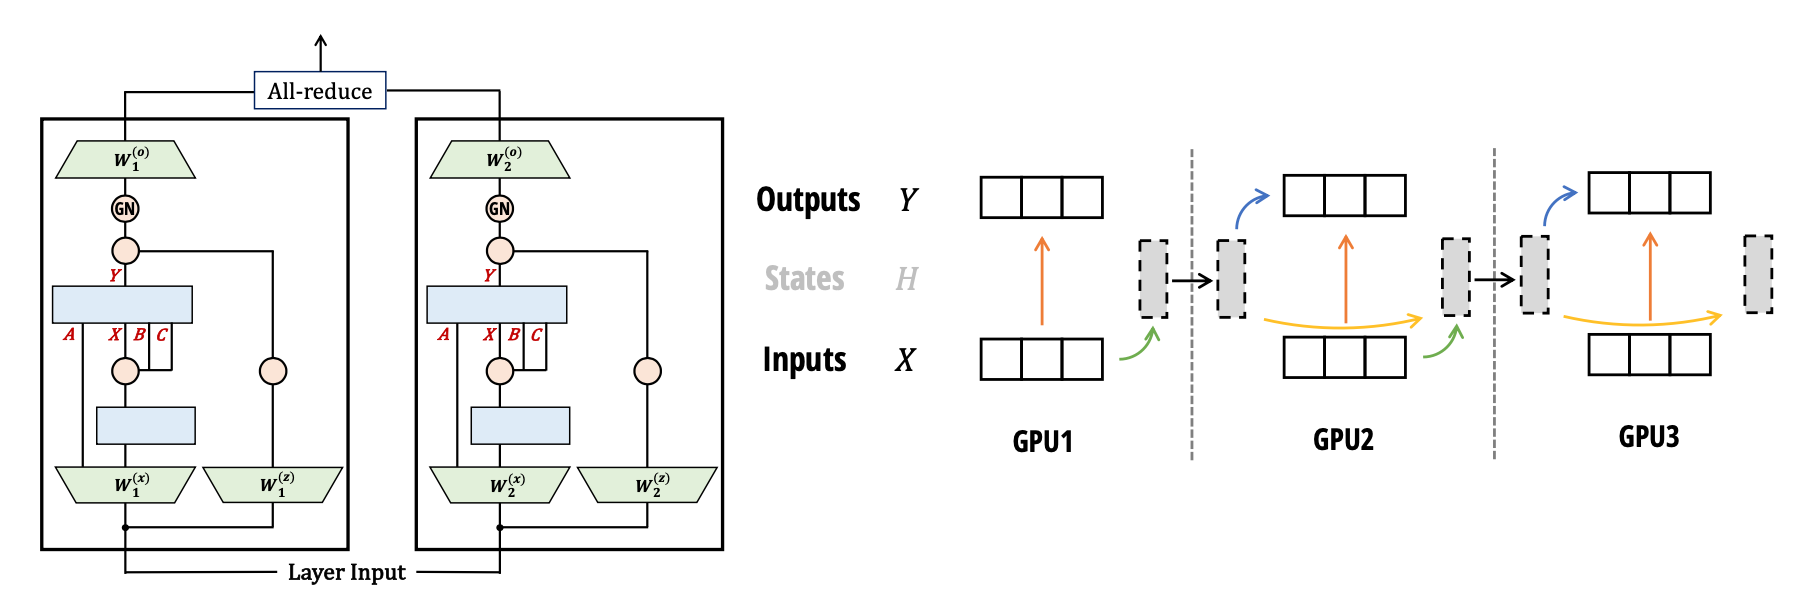
\includegraphics[width=1.0\linewidth]{images/mamba2_gpu.png}
    \caption{Parallélisme avec le bloc Mamba-2 \citep{dao2024mamba2}.}
    \label{fig:mamba2_gpu}
\end{figure}

À gauche : parallélisme tensoriel. Les matrices de projection d’entrée $\mathcal{W}^{(x)}$, $\mathcal{W}^{(z)}$ ainsi que la matrice de projection de sortie $\mathcal{W}^{(o)}$ sont divisées entre les dispositifs. Chaque tête SSM, correspondant à la transformation $(A, B, C, X) \mapsto Y$, est exécutée sur un seul GPU. La normalisation finale est assurée par une GroupNorm, ce qui permet d’éviter toute communication supplémentaire entre les dispositifs. Une unique opération \textit{all-reduce} est effectuée à la fin de chaque couche, à l’image de ce qui est réalisé dans les blocs MLP ou attention des Transformers. A droite : parallélisme de séquence (ou de contexte). Une approche similaire à l’algorithme SSD est suivie. La séquence d’entrée est découpée selon la dimension temporelle et répartie entre plusieurs dispositifs. Chaque appareil est chargé de calculer l’état caché correspondant à sa portion de séquence, puis cet état est transmis au GPU suivant.

\paragraph{Parallélisme de séquence} Pour les très longues séquences, les entrées et activations peuvent être réparties entre différents GPU le long de la dimension temporelle. Deux grandes techniques sont alors appliquées.\\

D'abord, le parallélisme de séquence (SP) pour les opérations résiduelles et de normalisation. Cette technique, initialement proposée par \citep{korthikanti2023}, consiste à décomposer le \textit{all-reduce} classique du TP en deux étapes : un \textit{reduce-scatter} suivi d’un \textit{all-gather}. En remarquant que les opérations résiduelles et de normalisation sont appliquées de manière identique sur chaque GPU d’un même groupe TP, les activations sont découpées selon la longueur de la séquence, puis les étapes suivantes sont réalisées : \textit{reduce-scatter}, opérations résiduelles et de normalisation localisées, puis \textit{all-gather}.\\

Ensuite, le parallélisme de contexte (CP) pour les opérations de mélange de tokens (attention ou SSM). Ce parallélisme est également appelé parallélisme de séquence dans certains contextes. Pour les couches d’attention, plusieurs techniques ont été développées (ex. : Ring Attention \citep{liu2024ring, liu2023bandwidth}), impliquant des stratégies sophistiquées de répartition de charge \citep{brandon2023balanced}. Une difficulté principale réside dans le fait que chaque bloc de requêtes (queries) doit interagir avec tous les blocs de clés (keys), menant à une communication quadratique en fonction du nombre de dispositifs.\\

Avec les SSMs, cette difficulté est évitée. La séquence peut être simplement découpée : chaque GPU reçoit un état initial, effectue le calcul SSM sur sa portion de séquence, puis transmet l’état final au GPU suivant. Ainsi, la bande passante de communication est linéaire en fonction du nombre de dispositifs. Cette décomposition correspond exactement à la structure en blocs introduite dans l’algorithme SSD.\\

En s’appuyant sur la dualité structurée (SSD), Mamba-2 étend les capacités des SSMs en les reliant formellement aux architectures attentionnelles tout en maintenant une complexité linéaire. Par ses apports structurels et systèmes (parallélisme tensoriel et de séquence), Mamba-2 s’impose comme une alternative crédible aux Transformers dans les scénarios de traitement de séquences longues. Cependant, malgré ses nombreux avantages, l’architecture Mamba-2 reste coûteuse en ressources lors de l'entraînement de très grands modèles. C’est dans ce contexte qu'intervient Llamba, une déclinaison légère et distillable de Mamba-2, pensée pour combiner la rapidité d’inférence et la compacité des modèles tout en conservant les performances des grands modèles de type Llama. 

\subsection{Llamba}

L’émergence de Llamba, proposée par \citep{bick2025llamba}, marque une nouvelle étape dans l’évolution des modèles à espace d’état sélectifs adaptés au traitement de séquences longues. Alors que Mamba-2 avait déjà démontré qu’il était possible de concilier expressivité, efficacité séquentielle et parallélisation, Llamba va plus loin en répondant à un double enjeu : proposer une alternative concrète aux Transformers pour les grands modèles de langage, tout en rendant l’inférence plus légère et accessible pour des déploiements sur appareils grand public (edge devices). L'innovation majeure de Llamba réside dans son intégration explicite d’un protocole de distillation architecturale, appelé MOHAWK qui permet de transférer les représentations apprises par un enseignant (de type Llama) vers un élève récurrent reposant sur une version discrétisée de Mamba-2. Pour ce faire, une présentation des apports par rapport à Mamba-2 sera effectuée. Puis, une description approfondie du cadre MOHAWK, son fonctionnement mathématique. Ensuite, une formalisation du modèle Discrete Mamba-2, qui est la base Llamba, enfin, une analyse de l’architecture complète de Llamba dans ses différentes variantes (1B, 3B, 8B).

\subsubsection{Apports par rapport à Mamba-2}

Llamba repose sur un processus de distillation innovant appelé \textit{MOHAWK}, qui permet de transférer les connaissances de modèles Llama-3.x vers une architecture récurrente issue de Mamba-2. Ce mécanisme rend possible l'entraînement de Llamba avec moins de 0{,}1\% des données habituellement nécessaires, réduisant drastiquement les coûts de calcul. Une version modifiée de Mamba-2, dite \textit{Discrete Mamba-2}, est également introduite : elle se distingue par la suppression de la normalisation avant projection de sortie, le retrait de l'activation post-convolution, ainsi que l’élimination du paramètre de discrétisation $\Delta$, remplacé par une projection directe de la matrice $A$ depuis l'entrée.\\

Par ailleurs, Llamba adopte une structure modulaire alternée, combinant blocs Mamba et blocs MLP (inspirés des Transformers), ce qui permet de limiter la profondeur temporelle et d’accélérer les calculs. L’architecture intègre aussi un schéma multi-têtes étendu avec 32 têtes de dimension 64, 96 ou 128, et une taille d’état de 64, marquant une divergence par rapport au schéma MVA utilisé dans Mamba-2 tout en préservant une grande efficacité en inférence.\\

Ces adaptations structurelles ne suffisent toutefois pas, à elles seules, à garantir des performances comparables à celles des modèles enseignants de type Llama. Afin de tirer pleinement parti de l’architecture allégée de Llamba, un protocole de distillation dédié a été conçu. Celui-ci, baptisé MOHAWK, vise à transférer les dynamiques internes d’un modèle Transformer vers une architecture récurrente.

\subsubsection{MOHAWK : Matching Output Head and Activations With Knowledge}

Le schéma MOHAWK est un protocole de distillation architecturale visant à transférer efficacement les dynamiques internes d’un modèle enseignant (typiquement un Transformer comme Llama-3) vers un modèle élève récurrent tel que Llamba. Il se distingue des approches classiques par l’alignement explicite de plusieurs niveaux de représentations entre les deux architectures.\\

De nombreuses méthodes ont récemment été proposées pour distiller des modèles Transformers vers des architectures plus légères tout en préservant leurs performances. SUPRA \citep{mercat2024supra} propose de linéariser l’attention softmax en une forme d’attention linéaire en copiant les matrices de poids puis en ajustant par fine-tuning. LoLCATs \citep{zhang2024lolcats} introduit une méthode de transfert d’attention combinée à une adaptation bas-rang pour remplacer l’attention softmax par une attention linéaire, ce qui permet la création de modèles linéarisés à grande échelle plus efficaces. Wang et al. \citep{wang2025ssd} s’appuient sur la dualité espace d’état (SSD) de \citep{dao2024ssd} pour transférer les poids de projection linéaire des couches d’attention vers des modèles Mamba. Leurs expériences incluent des modèles hybrides combinant attention et SSM, montrant qu’un bon équilibre entre les deux préserve les performances tout en améliorant l’efficacité. Enfin, MOHAWK \citep{bick2024transformers} propose une distillation progressive alignant les représentations intermédiaires, permettant aux modèles sous-quadratiques d’exploiter les ressources d’entraînement des Transformers. Ces approches confirment la faisabilité de distiller efficacement des Transformers coûteux vers des modèles compacts aux performances compétitives.\\

Conformément au cadre MOHAWK \citep{bick2024transformers}, l’initialisation des modèles Llamba a été réalisée en paramétrant la couche convolutionnelle de chaque bloc Mamba comme un noyau identité (rendant son effet nul), et en configurant la connexion multiplicative comme un simple passage direct de l’entrée, ce qui revient à initialiser chaque bloc comme une fonction identité. Soient $\mathcal{T}$ le modèle enseignant (de type Llama) et $\mathcal{S}$ le modèle étudiant (Llamba, basé sur Mamba-2). Ces deux modèles sont des réseaux profonds composés de $L$ blocs successifs (numérotés $1,\dots,L$), chacun contenant un mélangeur de séquence (self-attention pour $\mathcal{T}$, couche SSM Mamba-2 pour $\mathcal{S}$) suivi d’autres transformations (par ex. MLP). Notons $h^T_l$ le vecteur d’état caché (hidden state) de l’enseignant à la sortie du $l$-ième bloc, et $h^S_l$ celui de l’étudiant au même niveau. En particulier, $h^T_0 = h^S_0 = x$ représente l’entrée du modèle (embeddings initiaux de la séquence de tokens d’entrée). Le vecteur de logits de sortie (scores non normalisés des probabilités de prédiction) est noté $z^T = \mathcal{T}(x)$ pour l’enseignant et $z^S = \mathcal{S}(x)$ pour l’étudiant. Chaque bloc $l$ du modèle enseignant est noté $\mathcal{T}_l$, avec paramètres $\Theta^T_l$, et de même $\mathcal{S}_l$ (paramètres $\Theta^S_l$) pour l’étudiant. L’ensemble des paramètres du modèle complet est $\Theta^T = {\Theta^T_l}{l=1}^L$ et $\Theta^S = {\Theta^S_l}{l=1}^L$. Le protocole MOHAWK (“Matching Output Head and Activations With Knowledge”) est un processus de distillation de connaissance multi-niveaux visant à apprendre $\Theta^S$ à partir de $\Theta^T$.

Trois étapes principales ont ensuite été mises en œuvre :

\newpage

\textbf{Orientation des matrices.} La première étape vise à aligner directement le mélangeur de séquence de l’étudiant avec celui de l’enseignant. Autrement dit, on souhaite que la transformation de séquence effectuée par la matrice SSM de Mamba-2 imite celle de la matrice de self-attention du Transformer. Formellement, notons $W^T_l(x)$ la matrice effective de mélange du bloc enseignant $\mathcal{T}_l$ pour une entrée $x$ donnée, et $W^S_l$ la matrice (paramétrée par $\Theta^S_l$) du mélangeur SSM de $\mathcal{S}_l$. (Dans le cas de l’attention, $W^T_l(x)$ dépend de $x$ car la matrice d’attention est calculée via les similarités requête-clé du token, alors que $W^S_l$ est une matrice fixe, dérivée des paramètres SSM. On utilise ici une entrée $x$ typique ou un échantillon de données pour représenter la matrice d’attention «matérialisée ».) L’objectif d’alignement matriciel s’écrit : trouver les paramètres $\Theta^S_l$ pour chaque couche $l$ minimisant l’erreur quadratique entre ces matrices :

\begin{equation}
\min_{\Theta^S_l} \; \mathcal{L}_{\text{mat},l} \quad \text{où} \quad \mathcal{L}_{\text{mat},l} \;=\; \mathbb{E}_{x \sim \mathcal{D}} \big\| W^T_l(x)\;-\;W^S_l(\Theta^S_l)\big\|_F^2~.
\end{equation}

\textbf{Alignement des états cachés.} Malgré l’accord obtenu au niveau des matrices de mélange, les sorties de bloc de $\mathcal{S}$ peuvent encore différer de celles de $\mathcal{T}$, à cause des autres composantes du bloc (normalisation, connexion résiduelle, MLP, etc.) ou d’erreurs d’approximation. L’étape 2 vise donc à aligner les représentations intermédiaires des deux modèles couche par couche. Pour chaque bloc $l$, on va ajuster $\Theta^S_l$ afin que le vecteur de sortie $h^S_l$ coïncide avec $h^T_l$ lorsque les deux reçoivent la même entrée. Plus précisément, on maintient l’entrée de $\mathcal{S}l$ égale à $h^T_{l-1}$ (on alimente la couche étudiante $l$ avec la sortie réelle de la couche $(l-1)$ de l'enseignant, évitant ainsi la propagation d’erreurs accumulées). On minimise alors la distance $\ell_2$ entre les sorties de bloc :

\begin{equation}
\min_{\Theta^S_l} \; \mathcal{L}_{\text{hid},l} \quad \text{où} \quad \mathcal{L}_{\text{hid},l} \;=\; \mathbb{E}_{h^T_{l-1}} \big\|\, h^T_l \;-\; h^S_l(\Theta^S_l\,;\; h^T_{l-1})\big\|_2^2~.
\end{equation}

Ici $h^T_l = \mathcal{T}_l(h^T_{l-1})$ est la sortie du $l$-ième bloc enseignant, et $h^S_l(\Theta^S_l; h)$ représente la sortie du bloc étudiant $l$ lorsqu’on lui fournit une entrée $h$. En pratique, $h^T_{l-1}$ est pris sur la distribution réelle des états de l'enseignant, c'est-à-dire le vrai $h^T_{l-1}$ pour chaque donnée d’entraînement, de sorte à respecter la dynamique d’entrée naturelle de la couche. On procède ainsi indépendamment pour chaque couche (couche gelée par couche, en quelque sorte), ce qui évite que l’optimisation d’un étage n’affecte les autres – un choix important pour la stabilité de l’alignement. En parallèle sur $l=1\dots L$, on ajuste les poids de sorte que chaque bloc étudiant reproduise l’état caché du bloc enseignant correspondant. Dans le cas de Llamba (Mamba-2), on a au préalable modifié ou initialisé certains composants pour faciliter cet alignement complet : par exemple, on fixe le coefficient de gating interne à 1 (pour neutraliser son effet) et on supprime la normalisation juste avant la projection de sortie, ces éléments n’ayant pas d’équivalent direct dans le bloc self-attention de l'enseignant. Ainsi, l’étape 2 aboutit à des blocs $\mathcal{S}_l$ dont l’output est très proche de celui des blocs $\mathcal{T}_l$ respectifs (en norme Euclidienne), couche par couche. En d’autres termes, toutes les activations intermédiaires majeures de l’étudiant sont alignées sur celles du professeur. Cet alignement des états cachés constitue une forme de distillation intermédiaire qui prépare l’étape finale de raffinage global.\\

\textbf{Transfert de poids et distillation des connaissances.} Le transfert initial concerne les poids des MLPs, les couches de normalisation, les embeddings d’entrée et la tête de sortie. Contrairement à des travaux antérieurs \citep{wang2025ssd, bick2024transformers}, les poids MLP ne sont pas figés, mais optimisés avec le même taux d’apprentissage que les couches de mélange. Lors de la distillation, chaque modèle Llamba est aligné avec son enseignant via une perte d'entropie croisée appliquée aux logits. Une fois cette phase stabilisée, une distillation finale est opérée sur les jetons restants à partir de Llama-3.1-70B-Instruct.\\

Après les deux premières phases, l’architecture étudiante a hérité de la structure de l'enseignant et produit des activations comparables couche par couche. La troisième étape effectue une distillation de bout en bout des prédictions du modèle, tout en transférant certains paramètres restants du professeur. On initialise cette phase en copiant directement dans $\mathcal{S}$ les poids du professeur pour lesquels une correspondance directe existe : typiquement les poids des MLPs de chaque bloc, les matrices de normalisation (LayerNorm), les embedding initiaux des tokens, et la couche de sortie (tête language model pour les logits). Notons $\Theta^S_{\text{MLP}} \leftarrow \Theta^T_{\text{MLP}}$ ce transfert (l’étudiant hérite des MLP de l'enseignant, etc.). Après ce transfert de poids, l’entraînement final consiste à ajuster l’ensemble du modèle étudiant par distillation des logits de l'enseignant, afin d’affiner les petits écarts restants et d’améliorer les performances finales. Plus précisément, on entraîne $\mathcal{S}$ en minimisant la perte de distillation $\mathcal{L}_{KD}$ définie comme la cross-entropie entre la distribution de sortie de l’étudiant et celle de l’enseignant (pour les mêmes entrées). Par exemple, si $p^T(y|x) = \operatorname{Softmax}(z^T)$ est la distribution de probabilité sur le prochain token $y$ prédite par l'enseignant et $p^S(y|x) = \operatorname{Softmax}(z^S)$ celle de l’étudiant, on minimise :

\begin{equation}
\mathcal{L}_{KD} \;=\; \mathbb{E}_{x \sim \mathcal{D}} \Big[ H\big(p^T(\cdot|x),\; p^S(\cdot|x)\big) \Big] \;=\; \mathbb{E}_{x}\Big[-\sum_{y} p^T(y|x)\, \ln p^S(y|x)\Big]~.
\end{equation}

où $H(q,p)$ est l’entropie croisée. Cette optimisation se fait sur un grand corpus non étiqueté (p. ex. extraits de texte) pour lequel l'enseignant fournit des prédictions servant de cible pour l’élève. L’ensemble des paramètres $\Theta^S$ est affiné par descente de gradient en vue de reproduire au mieux les logits du professeur (distillation classique type Hinton et al., 2015). On obtient ainsi en fin d’étape 3 un modèle $\mathcal{S}$ dont les sorties $z^S$ approchent la distribution des sorties $z^T$ sur la distribution d’entraînement. Notons que, durant cette phase, il est possible de garder certains paramètres figés. Par exemple, on a constaté expérimentalement qu’on pouvait geler les poids des MLP du student tout en conservant une performance optimale. Cela s’explique par le fait que les MLP capturent une grande partie du savoir préentraîné de l'enseignant ; en les transférant tels quels à l’étudiant, on peut réduire de plus de moitié le nombre de paramètres à entraîner pendant la distillation finale, tout en évitant un oubli catastrophique éventuel de ces connaissances transférées.
.

\begin{demonstration}
On considère deux distributions de probabilité \(p^T(\cdot|x)\) et \(p^S(\cdot|x)\), respectivement les sorties normalisées (via softmax) d’un modèle enseignant et d’un modèle étudiant, conditionnellement à une entrée \(x \in \mathcal{D}\). La fonction de perte utilisée dans le cadre de la distillation des connaissances est l'espérance de l'entropie croisée entre ces deux distributions.

L'entropie croisée entre \(p^T\) et \(p^S\), pour une entrée donnée \(x\), est définie par :
\[
H\big(p^T(\cdot|x), p^S(\cdot|x)\big) = - \sum_{y} p^T(y|x) \ln p^S(y|x).
\]

En prenant l’espérance sur toutes les entrées \(x \sim \mathcal{D}\), on obtient la forme attendue de la perte de distillation :
\[
\mathcal{L}_{KD} = \mathbb{E}_{x \sim \mathcal{D}} \left[ H\left(p^T(\cdot|x), p^S(\cdot|x)\right) \right] = \mathbb{E}_{x \sim \mathcal{D}} \left[ - \sum_{y} p^T(y|x) \ln p^S(y|x) \right].
\]

Cette égalité découle directement de la linéarité de l'espérance et de la définition élémentaire de l'entropie croisée. Elle permet de formaliser la minimisation de la divergence entre les distributions de sortie de l’enseignant et de l’étudiant sur le support des données.
\end{demonstration}

Dans le cadre de Llamba, la phase 3 de distillation a été réalisée en deux temps avec deux enseignants successifs pour maximiser le transfert de connaissances. D’abord, on entraîne l’étudiant avec un enseignant initial de même taille (par ex. Llama-3B-Instruct pour Llamba-3B) durant la première partie de l’étape 3. Une fois la perte de distillation stabilisée (saturation du cross-entropie, indiquant que l’élève a presque atteint les performances du premier enseignant), on change de professeur et on continue l’entraînement de $\mathcal{S}$ sur le reste des données en utilisant un enseignant instructif de plus grande échelle (par ex. Llama-70B-Instruct). Cette distillation instructive supplémentaire permet d’incorporer les connaissances plus riches du grand modèle dans l’élève sans repartir de zéro. Formellement, si l’on note $p^{T_1}$ la distribution du premier enseignant et $p^{T_2}$ celle de l'enseignant instructif final, on minimise d’abord $\mathcal{L}{KD}[T_1] = \mathbb{E}{x} H(p^{T_1}, p^S)$ jusqu’à convergence, puis $\mathcal{L}{KD}[T_2] = \mathbb{E}{x} H(p^{T_2}, p^S)$ sur une nouvelle période d’entraînement. La condition de transition est donc l’atteinte d’un palier sur $\mathcal{L}_{KD}$ avec le premier enseignant (ou un nombre fixé de tokens d’entraînement consommés). Empiriquement, cette stratégie a montré son efficacité : par exemple, Llamba-8B a d’abord été distillé depuis Llama-3.1-8B-Instruct, puis affiné sur la fin du processus avec Llama-3.1-70B-Instruct, ce qui a amélioré ses performances zero-shot sans augmenter drastiquement le budget de données (12 milliards de tokens au total, soit <0,1\% des données de préentraînement usuelles).\\


Il est également possible de désigner $\mathcal{A}$ comme l'ensemble des paramètres alignés au sens des deux premières phases du cadre MOHAWK. Cela peut être vu comme une projection de l'espace de recherche vers une variété d'alignement pré-conditionnée :

\begin{equation}
\mathcal{A} = \left\{ \phi \ \middle| \ \left\| M_T(u) - M_{\phi}(u) \right\|_F \leq \varepsilon_1,\ \left\| B_T(u) - B_{\phi}(u) \right\|_2 \leq \varepsilon_2 \right\}
\end{equation}

Une spécificité importante du cadre est que la distillation ne se fait pas uniquement sur un enseignant fixe. On considère deux modèles enseignants successifs :

\begin{itemize}
  \item $T_1(x)$ : enseignant initial, typiquement un Llama-3.x
  \item $T_2(x)$ : enseignant instructif, par ex. Llama-3.1-70B-Instruct, appliqué aux jetons restants.
\end{itemize}
Le problème de distillation s'exprime alors sous la forme :

\begin{equation}
\min_\phi \ \mathbb{E}_{x \in \mathcal{D}_1} \mathcal{L}_{\text{CE}}(T_1(x), S_{\phi}(x)) + \mathbb{E}_{x \in \mathcal{D}_2} \mathcal{L}_{\text{CE}}(T_2(x), S_{\phi}(x))
\end{equation}

soit encore, 

\begin{equation}
\min_\phi \ \mathbb{E}_{x \in \mathcal{D}_1} \left[ -\sum_{i=1}^{d} T_{1,i}(x) \ln S_{\phi,i}(x) \right] + \mathbb{E}_{x \in \mathcal{D}_2} \left[ -\sum_{i=1}^{d} T_{2,i}(x) \ln S_{\phi,i}(x) \right]
\end{equation}

avec $\mathcal{D}_1$ les jetons utilisés pour la distillation de base et $\mathcal{D}_2$ les jetons finaux raffinés par un second enseignant plus robuste.\\

Cette approche est aussi dynamique, car elle dépend de la convergence de la première phase. Soit $t^*$ l'instant (ou nombre d'époques) où la perte saturée est atteinte pour $T_1$, alors le schéma est :

\begin{equation}
\phi_{t^*} = \arg\min_{\phi} \mathbb{E}_{x \in \mathcal{D}_1} \mathcal{L}_{\text{CE}}(T_1(x), S_{\phi}(x))
\end{equation}

puis, pour $t > t^*$,

\begin{equation}
\phi_{t} = \arg\min_{\phi} \mathbb{E}_{x \in \mathcal{D}_2} \mathcal{L}_{\text{CE}}(T_2(x), S_{\phi}(x))
\end{equation}

Ce qui revient à faire de l'optimisation par \textit{régime successif} selon un critère de saturation de la perte. Cette double phase permet de découpler le signal d'apprentissage selon la qualité des jetons ou des exemples.

\begin{demonstration}
On souhaite minimiser la fonction de perte d'entropie croisée entre la distribution de sortie d’un modèle enseignant $T(x)$ et celle d’un modèle étudiant $S_\phi(x)$, sous la contrainte que les paramètres $\phi$ de l’étudiant appartiennent à un sous-ensemble admissible $\mathcal{A}$ correspondant à un alignement structurel.

\[
\min_{\phi \in \mathcal{A}} \mathcal{L}_{\text{CE}}(T(x), S_\phi(x)) = -\sum_{i=1}^d T_i(x) \ln S_{\phi,i}(x)
\]

où $T(x), S_\phi(x) \in \Delta^{d-1}$ sont des distributions de probabilité sur un vocabulaire de taille $d$, obtenues via une softmax sur les logits respectifs des deux modèles.

L’ensemble admissible $\mathcal{A}$ est défini par des contraintes d’alignement entre les modules internes des deux architectures :

\[
\mathcal{A} = \left\{ \phi \ \middle| \ \|M_T(u) - M_\phi(u)\|_F \leq \varepsilon_1,\quad \|B_T(u) - B_\phi(u)\|_2 \leq \varepsilon_2 \right\}
\]

où $M_T$, $M_\phi$ désignent les matrices de mélange (self-attention ou SSM), et $B_T$, $B_\phi$ les blocs complets (comprenant normalisation, MLP, etc.).

Le problème s’inscrit donc dans le cadre de l’optimisation non-linéaire sous contrainte :

\[
\min_{\phi \in \mathbb{R}^p} \mathcal{L}_{\text{CE}}(T(x), S_\phi(x)) \quad \text{s.c.} \quad \phi \in \mathcal{A}
\]

L’entropie croisée entre deux distributions $p = (p_1, \ldots, p_d)$ et $q = (q_1, \ldots, q_d)$ est donnée par :

\[
H(p, q) = -\sum_{i=1}^d p_i \ln q_i
\]

Dans notre cas, $p = T(x)$ et $q = S_\phi(x)$, d’où :

\[
\mathcal{L}_{\text{CE}}(\phi) = -\sum_{i=1}^d T_i(x) \ln S_{\phi,i}(x)
\]

Le gradient de cette fonction de perte par rapport aux paramètres $\phi$ est obtenu par la règle de chaîne. On suppose que $S_\phi(x) = \operatorname{Softmax}(z_\phi(x))$, où $z_\phi(x)$ sont les logits produits par le modèle étudiant. Alors :

\[
\frac{\partial S_{\phi,i}(x)}{\partial z_{\phi,j}(x)} = S_{\phi,i}(x)(\delta_{ij} - S_{\phi,j}(x))
\]

ce qui donne, via rétropropagation :

\[
\nabla_\phi \mathcal{L}_{\text{CE}} = \nabla_\phi z_\phi(x)^\top (S_\phi(x) - T(x))
\]

où $J_\phi := \nabla_\phi z_\phi(x)$ est la jacobienne des logits.

Le problème de minimisation s’écrit alors comme suit :

\[
\begin{aligned}
\min_\phi & \quad \mathcal{L}_{\text{CE}}(\phi) \\
\text{s.c.} & \quad g_1(\phi) = \|M_T(u) - M_\phi(u)\|_F^2 - \varepsilon_1^2 \leq 0 \\
           & \quad g_2(\phi) = \|B_T(u) - B_\phi(u)\|_2^2 - \varepsilon_2^2 \leq 0
\end{aligned}
\]

On introduit alors le Lagrangien associé :

\[
\mathcal{L}(\phi, \lambda_1, \lambda_2) = \mathcal{L}_{\text{CE}}(\phi) + \lambda_1 g_1(\phi) + \lambda_2 g_2(\phi)
\]

Les conditions de Karush-Kuhn-Tucker (KKT) pour un minimum local $\phi^*$ s’écrivent :

\[
\nabla_\phi \mathcal{L}_{\text{CE}}(\phi^*) + \lambda_1 \nabla_\phi g_1(\phi^*) + \lambda_2 \nabla_\phi g_2(\phi^*) = 0
\]

avec $\lambda_1, \lambda_2 \geq 0$ et $g_i(\phi^*) \leq 0$.

Ainsi, le problème :

\[
\min_{\phi \in \mathcal{A}} \; -\sum_{i=1}^d T_i(x) \ln S_{\phi,i}(x)
\]

correspond à une distillation contrainte dans un espace réduit des paramètres, assurant que les représentations internes de l’étudiant restent alignées à celles du professeur, tout en minimisant la divergence entre leurs sorties.

\end{demonstration}

MOHAWK constitue le centre de la procédure de distillation, son efficacité repose également sur l’adoption d’une variante simplifiée et optimisée de l’architecture Mamba-2. C’est dans cette optique qu’a été introduit le modèle Discrete Mamba-2, dont la structure allégée facilite l’alignement des représentations tout en réduisant les coûts d’inférence. 

\subsubsection{Mamba-2 discrétisé}

Le modèle Discrete Mamba-2 est une simplification de l'architecture Mamba-2, conçue pour améliorer l'efficacité computationnelle et faciliter la distillation dans le cadre de Llamba. Il repose sur trois modifications. D'abord, une suppression de la couche de normalisation précédant la projection de sortie. Puis, une élimination de l'activation non-linéaire appliquée après la convolution depthwise. Enfn, un  remplacement du paramètre de discrétisation $\Delta$ par une projection directe de la matrice d'état $A$ depuis l'entrée :

\begin{equation}
A = f_A(u), \quad B = f_B(u), \quad C = f_C(u)
\end{equation}

Ces paramètres sont obtenus via des projections linéaires appliquées directement sur l'entrée $u$, ce qui permet d'éviter les dépendances intermédiaires coûteuses en mémoire. La chaîne de calcul devient donc :

\begin{align*}
x &= u \mathcal{W}^{(x)\top} \in \mathbb{R}^{L \times ed} \\
z &= u \mathcal{W}^{(z)\top} \in \mathbb{R}^{L \times ed} \\
A, B, C &= \text{LinearProjs}(u) \\
x_c &= \text{conv1d}(x) \\
y &= \text{SSM}_{A,B,C}(x_c) \\
y_g &= y \cdot \phi(z) \\
\text{out} &= y_g \mathcal{W}^{(o)\top}
\end{align*}

Ce design allégé conserve les propriétés séquentielles efficaces de Mamba-2 tout en rendant l'architecture plus facilement parallélisable et adaptée à la distillation et à l'inférence embarquée.\\

L’introduction du bloc Discrete Mamba-2 a permis de concevoir une architecture plus légère et mieux adaptée à la distillation. Toutefois, la performance finale de Llamba repose également sur une conception d’ensemble cohérente du modèle. 

\subsubsection{Architecture Llamba}

Contrairement aux architectures Mamba et Mamba-2 qui ont été conçues pour un entraînement depuis zéro, le modèle Llamba a été spécifiquement pensé dans une logique de distillation architecturale. Le cadre MOHAWK repose sur l'alignement progressif de sous-réseaux entre l'élève et l'enseignant, à différents niveaux de granularité. Cette contrainte a conduit Llamba à conserver la structure générale du modèle enseignant (Llama), avec pour principal changement la substitution du mécanisme d'attention par une alternative sous-quadratique.

\begin{definition}[Attention sous-quadratique]
L'attention sous-quadratique est toute opération d'attention appliquée à une séquence $\mathbf{X} \in \mathbb{R}^{L \times d}$ dont la complexité temporelle totale est strictement inférieure à celle de l'attention classique, c’est-à-dire :

\[
\text{Complexité temporelle} \quad \mathcal{C}(L) = o(L^2)
\]

Autrement dit, l'attention sous-quadratique remplace le produit matriciel $QK^\top \in \mathbb{R}^{L \times L}$ par une structure ou une approximation permettant un coût de calcul plus faible, typiquement $\mathcal{O}(L \ln L)$ ou $\mathcal{O}(L)$. Cela inclut notamment :
\begin{itemize}
    \item les attentions linéaires, il est supposé une factorisation du type :
    \[
    \text{Attention}(Q, K, V) = (Q \cdot \phi(K)^\top)(\phi(V))
    \]
    avec $\phi$ une fonction d'encodage choisie ;
    
    \item les convolutions causales, comme dans Mamba, où il y a :
    \[
    y_t = \sum_{s \leq t} K_{t,s} x_s
    \]
    avec $K$ semi-séparable ou exprimé comme un noyau convolutionnel ;
    
    \item les attentions creuses ou locales, où la matrice $QK^\top$ est masquée (localement ou hiérarchiquement), réduisant le nombre d’interactions à $w \ll L$ :
    \[
    \text{Complexité} = \mathcal{O}(L \cdot w)
    \]
\end{itemize}
\end{definition}


Les modèles Llamba-1B, 3B et 8B intègrent respectivement 16, 28 et 32 blocs résiduels de type Mamba-2, suivis de couches feed-forward. Ils conservent le tokenizer et le vocabulaire de Llama-3.1, avec des dimensions cachées de 2048, 3072 et 4096. Plusieurs modifications importantes les différencient toutefois de Mamba-2. Tout d'abord, des blocs MLP sont intercalés entre les blocs Mamba, contrairement aux architectures précédentes qui n’utilisaient que des blocs SSM. Ensuite, une variante multi-têtes de Mamba-2 est utilisée, avec 32 têtes de dimensions 64, 96 ou 128, et une taille d’état fixée à 64. Ce schéma remplace l’architecture MVA classique tout en conservant une faible complexité d’inférence.\\

Par ailleurs, la normalisation avant projection de sortie et l’activation après convolution sont supprimées, car ces non-linéarités, absentes dans les blocs d’attention, nuisent à l’alignement pendant la distillation. Enfin, la version "Discrete Mamba-2" est adoptée, dans laquelle la matrice $A$ est projetée directement depuis l’entrée, sans paramètre de discrétisation $\Delta$, afin d’approcher au mieux les mécanismes discrets de l’attention (\autoref{fig:llamba-bloc}).

\begin{figure}[H]
    \centering
    \begin{minipage}{0.45\textwidth}
        \centering
        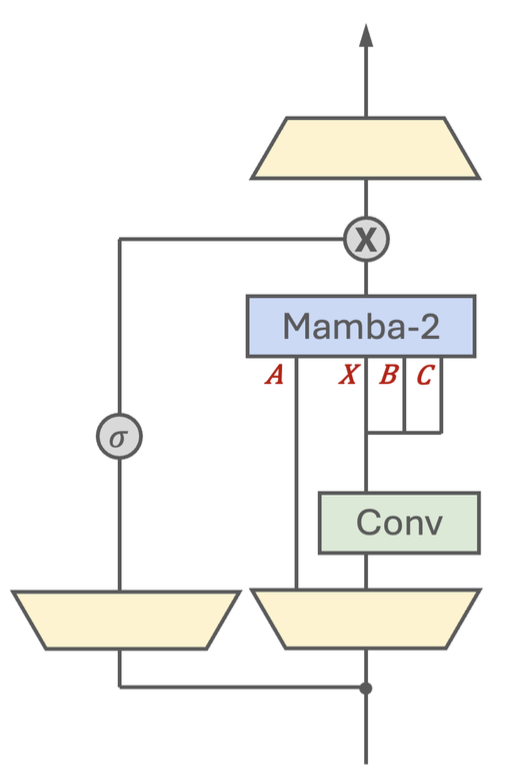
\includegraphics[width=\linewidth]{images/discrete_mamba2.png}
        \caption*{\justifying \small (a) Le bloc \textbf{Discrete Mamba-2} modifie l'architecture originale Mamba-2 en supprimant l'activation post-convolution et la normalisation pré-projection. Le paramètre de discrétisation $\Delta$ est éliminé, et la matrice $A$ est directement projetée depuis l'entrée.}
    \end{minipage}
    \hfill
    \begin{minipage}{0.45\textwidth}
        \centering
        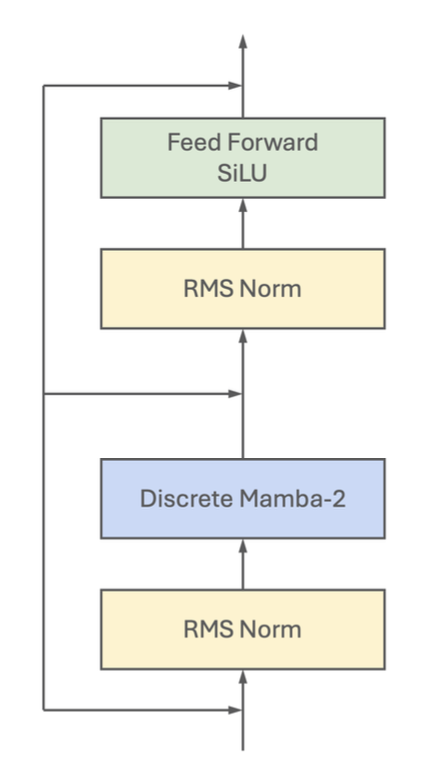
\includegraphics[width=\linewidth]{images/llamba_block.png}
        \caption*{\justifying \small (b) Les modèles \textbf{Llamba-1B, 3B, 8B} adoptent une structure dérivée de leurs enseignants Llama. Chaque bloc est composé de deux sous-blocs résiduels : (1) normalisation RMS suivie d’un bloc Discrete Mamba-2, et (2) normalisation RMS suivie d’une couche feed-forward.}
    \end{minipage}
    \caption{Comparaison entre le bloc Discrete Mamba-2 et l’architecture des modèles Llamba \citep{bick2025llamba}.}
    \label{fig:llamba-bloc}
\end{figure}

Ces modifications ne facilitent pas seulement la distillation, elles améliorent également l'efficacité de l'entraînement. L'alternance avec des MLPs permet de réduire le nombre de couches de mélange temporel, ce qui accélère les calculs. De plus, l’absence de normalisation allège les opérations de synchronisation inter-GPU, rendant l’entraînement plus simple et plus rapide.\\

Les modèles Transformers, Mamba, Mamba-2 et Llamba constituent aujourd’hui une classe émergente d’architectures séquentielles capables de rivaliser avec les Transformers sur des tâches de modélisation de séquences longues, tout en conservant une complexité linéaire et une efficacité computationnelle remarquable. Leur ancrage mathématique dans les systèmes dynamiques linéaires à espace d’état, enrichis de mécanismes de sélection contextuelle et d’algorithmes structurés comme la dualité SSD, permet de concevoir des modèles à la fois expressifs, interprétables et adaptés aux contraintes de mémoire et d'inférence. Dans ce travail, ces modèles sont mobilisés dans un objectif précis : construire un indicateur continu de forward guidance (FG) à partir des discours de politique monétaire. Grâce à leurs propriétés de généralisation sur séquences longues et à leur capacité à moduler dynamiquement l’information, ils fournissent une base robuste pour extraire un signal latent reflétant l’orientation expansionniste ou restrictive du discours de la BCE.\\

Cependant, pour étudier l’effet de cette forward guidance sur le stress systémique par le CISS, une autre classe de modèles s’avère nécessaire. Il s’agit désormais de modéliser des relations temporelles entre les variables, en intégrant à la fois des dynamiques séquentielles et une incertitude potentiellement non gaussienne. C’est dans ce contexte que s’inscrit la suite de ce mémoire qui introduit deux familles de réseaux neuronaux adaptées à la modélisation de séries temporelles : les modèles LSTM, largement utilisés pour capturer des dépendances longues, et les auto-encodeurs Wasserstein, qui permettent une modélisation probabiliste et générative utile pour l’analyse contrefactuelle et la quantification des incertitudes.

\section{Modèles neuronaux de séries temporelles : LSTM et WAE}

Dans le cadre de ce mémoire, deux familles de modèles neuronaux adaptés aux séries temporelles vont être mobilisées, chacune apportant une perspective complémentaire sur la dynamique des phénomènes étudiés. Il s’agit, d’une part, des réseaux Long Short-Term Memory (LSTM), qui prolongent les réseaux récurrents classiques en y intégrant des mécanismes de mémoire interne permettant de capturer les dépendances à long terme de manière stable et contrôlée. Grâce à l’introduction de portes multiplicatives, ces modèles sont capables de filtrer l’information temporelle de façon adaptative, ce qui les rend particulièrement efficaces dans des contextes où la mémoire joue un rôle crucial. D’autre part, les WAE seront utilisés dans une approche de transport optimal comme solution à la structuration de l'espace latent et non supervisée. Leur capacité à projeter les données séquentielles dans un espace latent structuré et régularisé permet non seulement d’extraire des représentations compactes des trajectoires temporelles, mais également de modéliser de manière implicite des régimes dynamiques sous-jacents, en capturant la variabilité des structures temporelles du stress systémique.\\

L’architecture des LSTM est d'abord détaillée, en mettant l’accent sur la dynamique interne des cellules, les mécanismes de contrôle par portes multiplicatives, ainsi que sur la capacité de ces réseaux à maintenir et exploiter une mémoire à long terme sans souffrir de gradient évanescent. Ce paragraphe soulignera également leur pertinence pour la modélisation de séries temporelles économiques à forte persistance. Le cadre théorique des WAE sera ensuite présenté à travers la formulation de la distance de Wasserstein, la régularisation entropique et l'algorithme de Sinkhorn. L’architecture encodeur-décodeur ainsi que le procédé de réparamétrisation, nécessaire à l’apprentissage différentiable des représentations latentes, seront également exposés. L’objectif est de combiner ces approches afin de modéliser de manière précise, robuste et complémentaire l’impact de la politique monétaire, en particulier de la forward guidance, sur le stress systémique au sein de la zone euro.

\subsection{Réseaux Long Short-Term Memory}

Les réseaux LSTM sont un type de réseaux neuronaux récurrents conçus pour apprendre des dépendances à long terme dans des séquences. Introduits par \citep{hochreiter1997long}, ils ont constitué l’une des premières solutions efficaces au problème du \textit{gradient évanescent} dans les RNN classiques \citep{hochreiter1997long, d2l2020}. L’idée principale du LSTM est d’ajouter à l’architecture récurrente une cellule de mémoire interne dotée de connexions récurrentes à poids fixe égal à 1, ce qui permet au gradient de se propager sur de très longues séquences sans s’annuler ni exploser \citep{d2l2020}. En pratique, chaque cellule de mémoire LSTM conserve un état interne $c_t$ (aussi appelé \textit{état de cellule}) qui joue le rôle de mémoire à long terme, ainsi qu’un état caché $h_t$ (mémoire à court terme ou sortie de la cellule).

\subsubsection{Présentation de la structure des LSTM}

L’architecture d’un LSTM repose sur l’enchaînement de cellules identiques dans le temps, chacune recevant une entrée $x_t$ et transmettant un état caché $h_t$ ainsi qu’un état mémoire $c_t$ à la cellule suivante. L’ensemble du réseau forme une structure récurrente dans laquelle le signal peut être propagé à travers des dizaines ou centaines de pas de temps, tout en conservant la stabilité du gradient grâce aux mécanismes internes de mémoire, le fonctionnement d'une cellule schématiquement est consigné en \autoref{fig:lstm_schema}.\\

\begin{figure}[H]
    \centering
    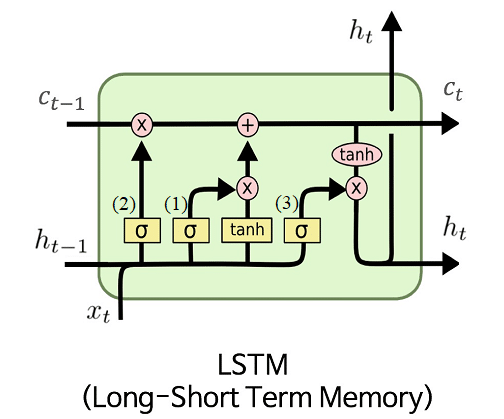
\includegraphics[width=0.5\linewidth]{images/lstm_schema.png}
    \caption{Schéma d'une cellule LSTM.}
    \label{fig:lstm_schema}
\end{figure}

Les cellules peuvent être empilées pour former des architectures multi-couches (\textit{deep LSTM}) \autoref{fig:lstm_schema_replicate}., permettant d’augmenter la capacité du modèle à extraire des représentations hiérarchiques. 

\begin{figure}[H]
    \centering
    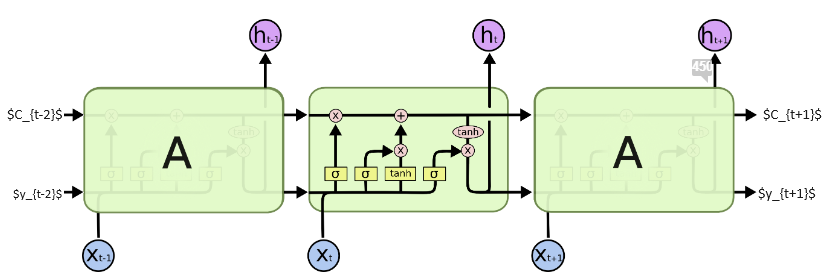
\includegraphics[width=1\linewidth]{images/lstm_relicates_cells.png}
    \caption{Schéma de fonctionnement du LSTM.}
    \label{fig:lstm_schema_replicate}
\end{figure}

De plus, des variantes bidirectionnelles \autoref{fig:lstm_bidirectionnel} peuvent être utilisées pour traiter les séquences dans les deux sens temporels, en concaténant les sorties forward et backward. 

\begin{figure}[H]
    \centering
    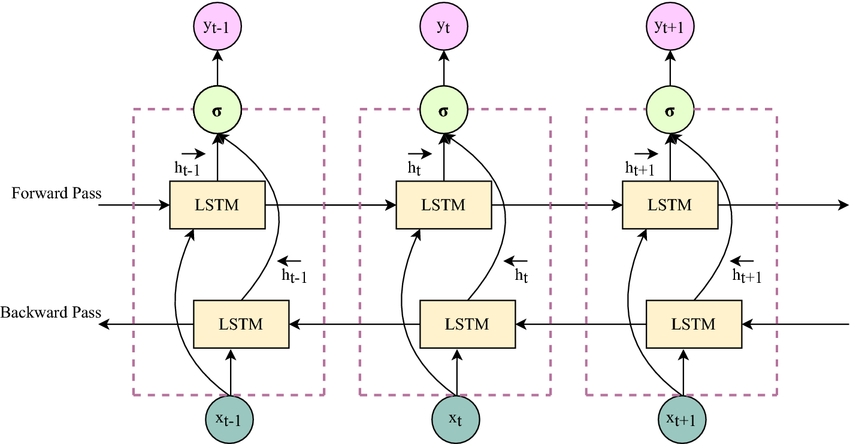
\includegraphics[width=1\linewidth]{images/lstm_bidirectionnel.png}
    \caption{Schéma de fonctionnement du LSTM Bidirectionnel.}
    \label{fig:lstm_bidirectionnel}
\end{figure}

L’ensemble de la structure est entraîné bout-à-bout via rétropropagation dans le temps, et peut être combiné à d’autres modules neuronaux dans des architectures plus complète, comme les autoencodeurs séquentiels, les modèles de séquence à séquence (seq2seq) ou les réseaux hybrides avec attention.\\

Après avoir présenté l’architecture générale des réseaux LSTM et leur capacité à modéliser des séquences via l’empilement de cellules récurrentes, il convient désormais d’examiner plus en détail le fonctionnement interne de ces cellules. En particulier, les mécanismes de mémoire contrôlée reposent sur des structures de portes multiplicatives.

\subsubsection{Cellules mémoires}

Pour contrôler l’accès et la modification de la mémoire interne $c_t$, le LSTM utilise des mécanismes de porte multiplicatives qui filtrent et régulent le flux d’information \citep{d2l2020}. Classiquement, une cellule LSTM est dotée de trois portes principales :

\begin{itemize}
    \item \textbf{Porte d’entrée (input gate)}, notée $i_t$, elle détermine dans quelle mesure l’information nouvelle (à l’instant $t$) doit être ajoutée à l’état interne de la cellule. Autrement dit, elle filtre l’apport de la nouvelle entrée dans la mémoire.
    
    \item \textbf{Porte d’oubli (forget gate)}, notée $f_t$, elle décide quelle fraction de l’état interne précédent $c_{t-1}$ doit être oubliée (remise à zéro) au temps $t$. Une valeur proche de 1 signifie que la cellule conserve complètement l’ancienne mémoire, tandis qu’une valeur proche de 0 signifie qu’elle l’efface. Historiquement, cette porte d’oubli a été introduite ultérieurement par Gers et al. (1999) pour permettre à la cellule de réinitialiser son contenu de manière apprise \citep{gers1999learning}.
    
    \item \textbf{Porte de sortie (output gate)}, notée $o_t$, elle module l’extraction de l’information depuis la cellule de mémoire vers l’état caché (et donc vers la sortie du LSTM). Elle décide quelle partie de la mémoire interne influencera la sortie $h_t$ de la cellule.
\end{itemize}

Ces portes sont implémentées par des neurones sigmoïdes (activation $\sigma$) produisant des coefficients dans $[0,1]$ qui multiplient (opération de Hadamard) les informations véhiculées \citep{d2l2020}. En plus des trois portes, la cellule LSTM calcule un nouveau contenu candidat $\tilde{c}_t$ pour la mémoire, à partir de l’entrée courante et de l’état caché précédent, via une activation $\tanh$ bornée entre $-1$ et $1$. Ce contenu candidat représente les nouvelles informations pouvant entrer en mémoire à $t$. Grâce aux portes d’entrée et d’oubli, le LSTM peut décider d’écraser une partie de son état interne par de nouvelles informations pertinentes ou au contraire de conserver des informations anciennes sur de longs intervalles de temps. Ce comportement peut être démontré de manière formelle dans un cas limite simple :

\begin{demonstration}
Soit l’équation de mise à jour de la mémoire :

\[
c_t = f_t \odot c_{t-1} + i_t \odot \tilde{c}_t
\]

Supposons que $f_t = \mathbf{1}$ (vecteur de 1) et $i_t = \mathbf{0}$ (vecteur de 0), alors :

\[
c_t = \mathbf{1} \odot c_{t-1} + \mathbf{0} \odot \tilde{c}_t = c_{t-1}
\]

Ainsi, la mémoire est exactement conservée à l’identique. Cela illustre la capacité du LSTM à maintenir l’information sur de longues durées sans altération.
\end{demonstration}

Ce mécanisme de mémoire contrôlée permet d’atténuer drastiquement le problème des gradients évanescents et d’apprendre des dépendances à long terme bien plus facilement qu’avec des RNN simples. La conception du LSTM fait que se rappeler des informations sur de longues durées devient le comportement par défaut du réseau, plutôt qu’une difficulté à surmonter \citep{colah2015lstm}. Les portes confèrent alors au LSTM sa capacité distinctive à filtrer, mémoriser ou oublier sélectivement l’information à chaque pas de temps. Pour en comprendre le fonctionnement précis, il est nécessaire de formaliser les équations internes qui gouvernent l’évolution de l’état mémoire et de l’état caché, et d’analyser les opérations élémentaires qui s’enchaînent au sein d’une cellule LSTM.

\subsubsection{Opérations internes d'un LSTM}

Formellement, à chaque pas de temps $t$, le LSTM reçoit en entrée un vecteur $x_t$ (par exemple, les observations de la série temporelle à l’instant $t$), ainsi que l’état caché $h_{t-1}$ et l’état de cellule $c_{t-1}$ issus du pas précédent. La cellule LSTM effectue alors les calculs internes suivants :

\begin{align*}
i_t &= \sigma\left(W_i x_t + U_i h_{t-1} + b_i\right) \quad &\text{(porte d’entrée)}\\
f_t &= \sigma\left(W_f x_t + U_f h_{t-1} + b_f\right) \quad &\text{(porte d’oubli)}\\
o_t &= \sigma\left(W_o x_t + U_o h_{t-1} + b_o\right) \quad &\text{(porte de sortie)}
\end{align*}

Chaque porte $i_t, f_t, o_t$ est un vecteur de même dimension que l’état caché, obtenu par une combinaison linéaire de l’entrée $x_t$ et de l’état caché précédent $h_{t-1}$, passée dans une fonction sigmoïde $\sigma(u) = \frac{1}{1 + e^{-u}}$ qui produit un facteur multiplicatif compris entre 0 et 1. Les matrices $W_*$, $U_*$ et les biais $b_*$ sont les paramètres appris du modèle.

Ensuite, la cellule calcule le contenu candidat $\tilde{c}_t$ susceptible de mettre à jour la mémoire interne :

\begin{equation}
\tilde{c}_t = \tanh\left(W_c x_t + U_c h_{t-1} + b_c\right) 
\end{equation}

où $\tanh(u) = \frac{e^u - e^{-u}}{e^u + e^{-u}}$ est la tangente hyperbolique, produisant des valeurs bornées entre $-1$ et $1$. Ce vecteur $\tilde{c}_t$ représente les nouvelles informations susceptibles d’être injectées dans la mémoire.

L’état interne de la cellule est alors mis à jour par pondération entre l’ancien état $c_{t-1}$ et le nouveau contenu :

\begin{equation}
c_t = f_t \odot c_{t-1} + i_t \odot \tilde{c}_t 
\end{equation}

où $\odot$ désigne le produit élément-par-élément (produit de Hadamard). Le vecteur $f_t$ contrôle la rétention de l’information ancienne (si $f_{t,j} \approx 1$, la composante $j$ de $c_{t-1}$ est conservée ; si $f_{t,j} \approx 0$, elle est oubliée), tandis que $i_t$ module l’intégration des nouvelles informations contenues dans $\tilde{c}_t$. Par exemple, si $f_t \approx \mathbf{1}$ et $i_t \approx \mathbf{0}$, alors $c_t \approx c_{t-1}$ : la mémoire est conservée parfaitement sur de longues séquences. Cette formulation présente un avantage crucial en termes de stabilité du gradient, comme le montre la dérivée suivante :


\begin{demonstration}
Considérons la dérivée partielle de $c_t$ par rapport à $c_{t-1}$ :

\[
c_t = f_t \odot c_{t-1} + i_t \odot \tilde{c}_t \quad \Rightarrow \quad
\frac{\partial c_t}{\partial c_{t-1}} = \frac{\partial (f_t \odot c_{t-1})}{\partial c_{t-1}} = \text{diag}(f_t)
\]

La dérivée est simplement une matrice diagonale avec les composantes de $f_t$ sur la diagonale. Si $f_t$ reste proche de 1, alors le gradient à travers le temps n’est pas atténué, ce qui explique pourquoi le LSTM évite le problème du gradient évanescent rencontré dans les RNN classiques.
\end{demonstration}

Enfin, l’état caché $h_t$ est calculé à partir de la mémoire mise à jour et de la porte de sortie :

\begin{equation}
h_t = o_t \odot \tanh(c_t) 
\end{equation}

La porte $o_t$ agit comme un filtre dynamique qui décide quelles composantes de l’état mémoire $c_t$ doivent être transmises à la sortie $h_t$ de la cellule. Lorsque $o_{t,j} \approx 0$, la composante $j$ de la mémoire est bloquée ; lorsqu’elle est proche de 1, elle est pleinement transmise. L’état caché $h_t$ est ensuite utilisé pour prédire l’observation suivante ou pour alimenter la couche suivante, et il sert également d’entrée au pas de temps suivant $(t+1)$. 

En résumé, ces équations décrivent le fonctionnement interne d’une cellule LSTM standard. Les fonctions d’activation sigmoïde et $\tanh$ régulent l’échelle des activations et facilitent la rétropropagation du gradient. Lors de l'entraînement, les paramètres $\{W_*, U_*, b_*\}$ sont ajustés par rétropropagation dans le temps tronquée (BPTT, \textit{Backpropagation Through Time}) pour minimiser une fonction de coût adaptée à la tâche (par exemple, l’erreur de prédiction d’une série temporelle).

Grâce à ces mécanismes de portes adaptatives, le LSTM peut apprendre à oublier, mémoriser et exploiter sélectivement les informations, ce qui le rend extrêmement performant pour modéliser des dépendances à long terme dans les données séquentielles \citep{greff2017lstm}. De nombreuses études ont confirmé l’efficacité des LSTM dans des domaines variés tels que la reconnaissance vocale, la traduction automatique, ou encore les séries temporelles économiques et financières \citep{greff2017lstm}.\\

En définitive, les réseaux LSTM permettent bien la modélisation de séries temporelles, en particulier lorsqu’il s’agit de capturer des dépendances à long terme. Grâce à l’introduction de cellules mémoire et de portes multiplicatives, ils permettent de contrôler finement le flux d’information au sein du réseau, tout en évitant les problèmes classiques de gradient évanescent qui affectent les architectures récurrentes standards. Leur capacité à apprendre des représentations dynamiques profondes et à conserver des informations sur de longues séquences en fait un outil important dans ce cas, notamment pour l’orientation de la politique monétaire ou l’évolution du stress systémique. Toutefois, malgré leur expressivité, les réseaux LSTM demeurent fondamentalement déterministes et n’intègrent pas, par construction, une modélisation explicite de l’incertitude ou des structures latentes sous-jacentes aux données. Afin de surmonter cette limite et de capturer la variabilité inhérente aux régimes dynamiques du stress systémique, il devient pertinent de s’appuyer sur des modèles génératifs probabilistes. 

\subsection{Wasserstein AutoEncoders}

Les Wasserstein Auto-Encoders (WAE) forment une famille récente de modèles génératifs à variables latentes qui visent à combiner les atouts des autoencodeurs variationnels (VAE) et des réseaux adverses génératifs (GAN). Introduits par \citep{tolstikhin2018wasserstein}, les WAE proposent un nouvel objectif d’apprentissage fondé sur la distance de Wasserstein entre la distribution générée par le modèle et la distribution réelle des données. Contrairement aux VAE classiques, dont l’apprentissage maximise une borne inférieure du log-vraisemblance (ELBO) et impose une contrainte point-par-point entre la distribution a posteriori $Q(Z|X)$ et le prior $P_Z$, les WAE cherchent à minimiser directement une mesure de divergence globale entre la distribution des données $P_X$ et la distribution du modèle $P_G$. Cette approche induit un terme de régularisation différent de celui des VAE, encourageant la distribution agrégée des codes latents (c’est-à-dire la loi de $Z$ lorsque $X$ suit la loi des données) à coïncider avec la loi a priori choisie . En pratique, les WAE conservent de nombreux avantages des VAE (une architecture encodeur-décodeur stable, un entraînement généralement facile à optimiser, et un espace latent structuré propice à l’interpolation) tout en générant des échantillons de meilleure qualité visuelle (par exemple mesurée par le score FID).\\

L’idée des WAE découle en partie des limitations observées avec les VAE et les GAN traditionnels. Les VAE ont une fondation théorique élégante mais ont tendance à produire des échantillons flous dans le cas de données complexes comme les images naturelles . Ce problème est lié à leur critère d’entraînement : la minimisation de la divergence de Kullback-Leibler (KL) entre la distribution postérieure $Q(Z|X)$ et le prior $P_Z$ pour chaque point d’entraînement. En forçant chaque encodage individuel à suivre la même distribution $P_Z$, le VAE contraint fortement l’allocation de l’espace latent et peut provoquer un chevauchement des codes latents associés à des données différentes (on parle alors de « holes » dans l’espace latent). Ce phénomène est illustré par la figure ci-dessous : chaque point de données (cercles blancs dans l’espace $X$) est encodé en une distribution latente (zones rouges autour des triangles verts dans l’espace $Z$) que le VAE tente de forcer à coïncider avec le prior $P_Z$ (zone bleue) individuellement. À mesure de l’entraînement, ces distributions encodées pour chaque exemple se superposent de plus en plus, si bien que certaines régions latentes (par exemple autour du triangle vert central) deviennent admissibles pour reconstruire plusieurs exemples différents, ce qui entre en conflit avec le caractère déterministe du décodeur (un même code $z$ ne pouvant reconstruire qu’un seul $x$)

\begin{figure}[H]
    \centering
    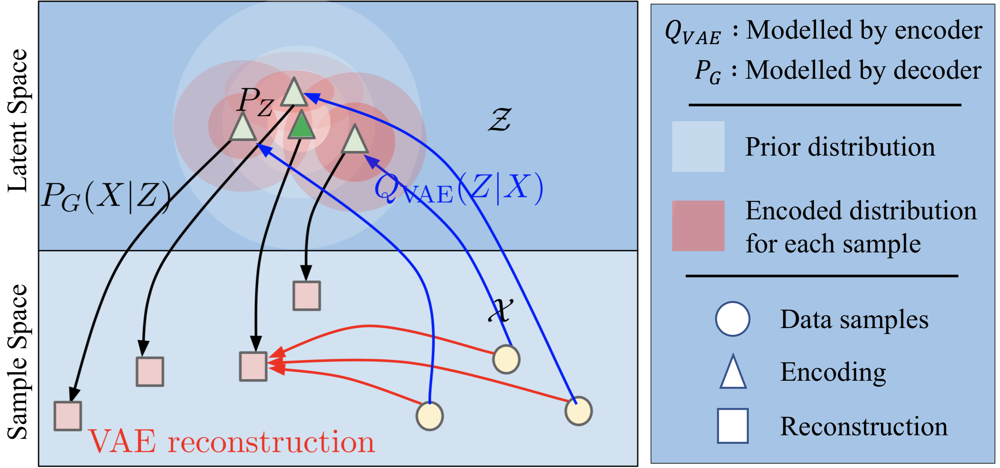
\includegraphics[width=1.0\linewidth]{images/pb_vae.png}
    \caption{\justifying Illustration du problème des VAE : en voulant faire matcher la distribution latente de chaque exemple (zones rouges) au prior global $P_Z$ (bleu), les encodages de différents points finissent par se chevaucher. Un code latent dans une région de chevauchement (triangle vert) serait alors considéré comme valide pour plusieurs données d’entraînement, alors que le décodeur ne peut en reconstruire qu’une seule, d’où un compromis qui dégrade la reconstruction.}
    \label{fig:enter-label}
\end{figure}

Plus généralement, l’emploi de divergences de type $f$-divergence (KL, divergence de Jensen-Shannon, etc.) pour ajuster des modèles génératifs peut poser problème lorsque le support des distributions ne coïncide pas exactement – situation fréquente lorsque les données $X$ sont concentrées sur des variétés de dimension inférieure dans l’espace ambient. Dans de tels cas, les $f$-divergences « maxent » à une valeur constante (par exemple la KL diverge vers $+\infty$ si $P_X$ n’est pas absolument continue par rapport à $P_G$), ce qui empêche d’obtenir un gradient utile pour l’apprentissage. À l’inverse, la distance de Wasserstein (issue de la théorie du transport optimal) définit une topologie beaucoup plus faible, c’est-à-dire qu’elle reste sensible aux différences entre distributions même lorsque celles-ci n’ont pas de support commun. En particulier, la distance de Wasserstein peut fournir un signal de gradient non nul pour entraîner un générateur même si les échantillons générés ne couvrent qu’une partie du support des données – un avantage crucial pour éviter le « mode collapse » souvent rencontré avec les GAN classiques. Ces considérations ont motivé l’émergence de nouvelles méthodes alliant autoencodeurs et distances de Wasserstein, notamment l’Autoencodeur Adversarial (Adversarial Auto-Encoder, AAE) de \citep{makhzani2016adversarial} et le WAE \citep{tolstikhin2018wasserstein}. Le WAE généralise d’ailleurs l’AAE : avec un coût de reconstruction quadratique et un régulateur adversarial, le WAE se confond exactement avec l’AAE, fournissant ainsi une première justification théorique du fait que l’AAE minimise effectivement une distance de Wasserstein entre $P_X$ et $P_G$ (en l’occurrence $W_2$).\\

le WAE propose de relâcher la contrainte imposée par le VAE sur chaque encodage individuel, en n’exigeant plus que la distribution agrégée des codes latents $Q_Z$ corresponde au prior $P_Z$, plutôt que chaque $Q(Z|X!=!x)$ pris isolément. L’encodeur a ainsi davantage de liberté pour disposer les représentations latentes des différentes observations à des emplacements distincts, ce qui facilite une reconstruction précise de chaque donnée (réduction du compromis entre reconstruction et régularisation). Le coût de reconstruction (erreur de reconstruction) demeure inchangé par rapport à un autoencodeur classique, mais le terme de régularisation est repensé : au lieu d’une KL locale, le WAE introduit un terme pénalisant l’écart entre $Q_Z$ et $P_Z$ dans l’espace latent, écart mesuré par la distance de Wasserstein ou une approximation de celle-ci. La figure suivante illustre l’approche WAE : toutes les données d’entraînement (cercles blancs) sont encodées en des points latents (triangles verts) dont la distribution globale $Q_Z$ (zone verte) est ajustée pour matcher le prior $P_Z$ (zone bleue), sans forcer chaque point individuellement.

\begin{figure}[H]
    \centering
    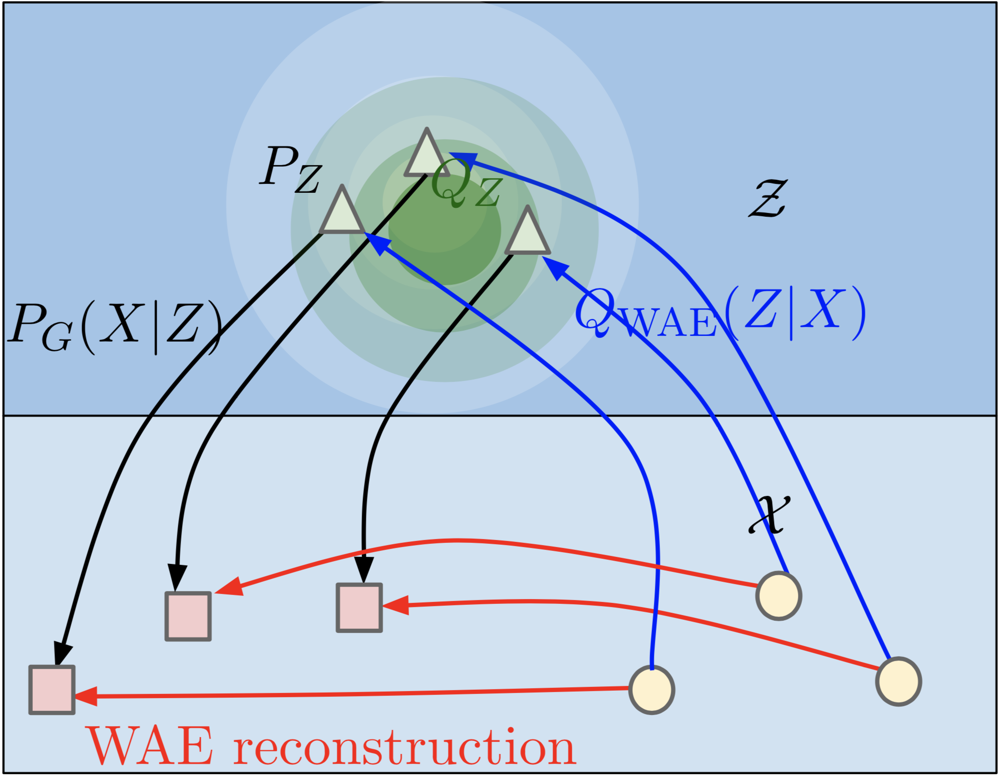
\includegraphics[width=0.7\linewidth]{images/wae.png}
    \caption{\justifying Principe du WAE : plutôt que de forcer chaque encodage individuellement à suivre le prior, on contraint la distribution agrégée de l’ensemble des codes latents $Q_Z$ (en vert) à coïncider avec la distribution prior $P_Z$ (en bleu). Un discriminateur entraîné dans l’espace latent peut servir à distinguer les codes issus de l’encodeur (échantillons de $Q_Z$) de ceux tirés du prior $P_Z$, et l’encodeur est entraîné à tromper ce discriminateur. Le décodeur, lui, est optimisé pour reconstruire les données ($X$) à partir des codes latents, via le coût de reconstruction (flèches rouges).}
    \label{fig:enter-label}
\end{figure}

Pour rappel, un VAE classique joint un \textit{encodeur} (réseau d’inférence) et un \textit{décodeur} (réseau génératif) reliés par un espace latent probabiliste représenté en \autoref{fig:vae_schema}, typiquement un espace de dimension réduite où $z$ suit une certaine loi \textit{a priori} simple (souvent une gaussienne standard). Intuitivement, l’encodeur associe à chaque donnée d’entrée une \textit{distribution} dans l’espace latent (plutôt qu’un point unique), et le décodeur échantillonne une variable latente depuis cette distribution pour générer une donnée reconstruite. Ce passage par une distribution au lieu d’un codage déterministe permet de \textit{généraliser} et d’\textit{éviter le surapprentissage}, tout en fournissant un cadre pour la génération aléatoire de nouvelles séquences ressemblant aux données d’entraînement.

\begin{figure}[H]
    \centering
    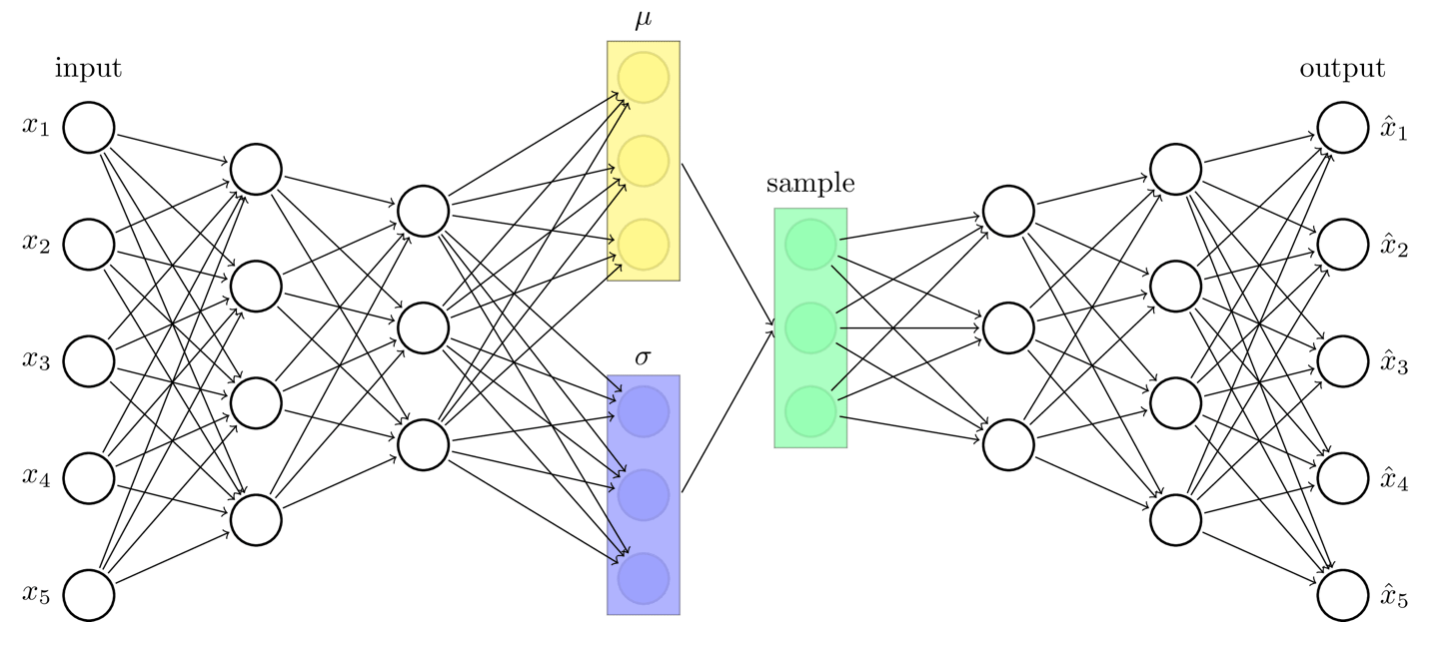
\includegraphics[width=1\linewidth]{images/vae.png}
    \caption{Schéma de fonctionnement d'un autoencodeur variationnel.}
    \label{fig:vae_schema}
\end{figure}

Pour ce faire, les fondements du Wasserstein Auto-Encoder sont d’abord introduits à travers la distance de Wasserstein, qui offre une mesure géométriquement plus pertinente que la divergence de Kullback–Leibler pour comparer des distributions de probabilité. Ensuite, la régularisation entropique du transport optimal est présentée, permettant de stabiliser et d’accélérer les calculs. Cette régularisation est ensuite reformulée dans le cadre discret, conduisant à l’algorithme de Sinkhorn qui fournit une solution efficace au problème régularisé. Enfin, l’architecture encodeur-décodeur du WAE est décrite, en précisant comment la distance de Wasserstein est utilisée pour régulariser l’espace latent dans un cadre d’apprentissage profond entièrement différentiable, adapté à la modélisation de séries temporelles.

\subsubsection{La distance de Wasserstein}

Considérons deux mesures de probabilité $p$ et $q$ sur $\mathbb{R}^k$ ayant un second moment fini – c’est-à-dire
$\displaystyle \int_{\mathbb{R}^k}\|x\|^{2}\,dp(x)<\infty$ et de même pour $q$. La distance de Wasserstein d’ordre 2 (ou coût quadratique de transport optimal) se définit alors par le problème de Kantorovich :
    
\begin{equation}
W_{2}^{2}(p,q)\;=\;
\min_{\Gamma\in\Pi(p,q)}
\int_{\mathbb{R}^k\times\mathbb{R}^k}\|x-y\|^{2}\,d\Gamma(x,y),
\end{equation}

où l’ensemble des plans de transport admissibles est

\begin{equation}
\Pi(p,q)\;=\;
\Bigl\{\Gamma\ge 0\;\bigm|\;
\forall\,A\subset\mathbb{R}^k,\;
\Gamma(A\times\mathbb{R}^k)=p(A),\;
\Gamma(\mathbb{R}^k\times A)=q(A)
\Bigr\}.
\end{equation}

Une mesure $\Gamma$ couple la masse de $p$ et celle de $q$ :
$\Gamma(dx,dy)$ indique quelle proportion de la masse initialement située en $x$ est déplacée vers $y$.
L’intégrale représente alors le coût total du déplacement lorsque déplacer une unité de masse de $x$ à $y$ coûte $\|x-y\|^{2}$. Le minimum porte sur tous les couplages compatibles avec les deux marginales ; le résultat est une véritable distance métrique sur l’espace $\mathcal{P}_{2}(\mathbb{R}^k)$ des lois à variance finie. Elle induit la topologie de la convergence faible plus convergence des seconds moments et possède les propriétés usuelles : positivité, symétrie, inégalité triangulaire, complétude.\\

L'existence (de la solution) et le caractère quadratique est possible si $p$ est absolument continue (par rapport à la mesure de Lebesgue), le minimum est atteint par un transport de Monge : il existe une application $\,T:\mathbb{R}^k\to\mathbb{R}^k$ telle que $T_{\#}p=q$ et $\displaystyle{W_{2}^{2}(p,q)=\int\|x-T(x)\|^{2}\,dp(x)}$. Sous ce coût quadratique, le théorème de Brenier assure que $T$ est le gradient d’une fonction convexe : $T=\nabla\varphi$. Dans le cas général (supports quelconques, mesures discrètes), le problème doit être résolu au niveau du couplage $\Gamma$. En général, le plan optimal $\Gamma^$ n’est pas forcément déterministe (on est dans le cadre relâché de Kantorovich, plus général que le problème original de Monge), mais il existe sous des conditions faibles (par exemple si les distributions ont des supports compacts ou des moments finis). Trouver $\Gamma^$ revient à résoudre un programme linéaire de grande taille en dimension discrète, ou un problème variationnel en dimension continue, ce qui est coûteux (en $O(n^3)$ pour $n$ points) et délicat pour des applications sur de grands ensembles de données.

\subsubsection{Régularisation entropique}

Pour remédier aux difficultés de calcul du transport optimal classique, \citep{cuturi2013} a introduit la régularisation entropique de la distance de Wasserstein. L’idée est d’ajouter au problème de Kantorovich une pénalité favorisant la dispersion de $\Gamma$, sous la forme de l’entropie de Shannon de $\Gamma$. On définit ainsi, pour un paramètre $\varepsilon > 0$, une version régularisée du coût de transport :
\begin{equation}
W_{2,\varepsilon}^2(p,q) \;=\; \min_{\Gamma \in \Pi(p,q)} \Big\{\sum_{i,j} \Gamma_{ij}\,C_{ij} \;+\; \varepsilon \sum_{i,j} \Gamma_{ij}\ln(\Gamma_{ij})\Big\}\
\end{equation}

\begin{demonstration}[Lien avec l'entropie relative]
Soit \(\mu = p\otimes q\) et \(\gamma\ll\mu\).
Par Radon–Nikodym, il existe \(f=\frac{d\gamma}{d\mu}\)
tel que \(\displaystyle{\int h\,d\gamma = \int h\,f\,d\mu}\).
La divergence de Kullback–Leibler s’écrit
\[
\mathrm{KL}(\gamma\|\mu)
      =\int \ln f(x,y)\;d\gamma(x,y),
\]
et l’entropie relative
\(H(\gamma\|\mu):=-\mathrm{KL}(\gamma\|\mu)\)
vaut donc
\[
H(\gamma\|\mu)
      =-\int \ln\!\Bigl(\tfrac{d\gamma}{d(p\otimes q)}(x,y)\Bigr)\,d\gamma(x,y).
\]
Lorsque \(\mu=p\otimes q\), cette quantité mesure exactement la
déviation du plan \(\gamma\) vis-à-vis d’une indépendance parfaite
des marginales; prendre \(-\varepsilon H(\gamma\|\mu)\) revient donc à récompenser les couplages « flous ».
\end{demonstration}

\begin{demonstration}[Discrétisation de l'entropie relative]
Soient $p=(a_i)_{i=1}^{n}$ et $q=(b_j)_{j=1}^{m}$ les distributions
discrètes, et
$\gamma=(\gamma_{ij})$ un plan dans $\Pi(p,q)$.
Il vient
\(
(p\!\otimes\! q)(x_i,y_j)=a_i b_j
\)
et
\(
\gamma(x_i,y_j)=\gamma_{ij}
\),
d’où
\[
\frac{d\gamma}{d(p\otimes q)}(x_i,y_j)=\frac{\gamma_{ij}}{a_i b_j}.
\]
Ainsi
\[
H(\gamma)
= -\!\sum_{i,j}\gamma_{ij}\ln\!\Bigl(\tfrac{\gamma_{ij}}{a_i b_j}\Bigr)
= -\!\sum_{i,j}\gamma_{ij}\ln\gamma_{ij}
  +\sum_i a_i\ln a_i
  +\sum_j b_j\ln b_j.
\]
Or les deux derniers termes sont constants quand
$\gamma$ varie dans $\Pi(p,q)$.
On peut donc les omettre dans le problème d’optimisation, ce qui donne
\[
\boxed{\,H(\Gamma)\;=\;-\sum_{i,j}\gamma_{ij}\ln\gamma_{ij}\,}.
\]
\end{demonstration}

où $C_{ij} = |x_i - y_j|^2$ est la matrice des coûts quadratiques entre les $i$-èmes et $j$-èmes points de support de $p$ et $q$ respectivement. Ici $\Gamma_{ij}$ désigne la quantité de masse transportée de $x_i$ vers $y_j$, et les contraintes $\sum_j \Gamma_{ij}=p_i$, $\sum_i \Gamma_{ij}=q_j$ (i.e. $\Gamma\in\Pi(p,q)$) s’appliquent toujours. La pénalité entropique $ \varepsilon \sum_{i,j}\Gamma_{ij}\ln(\Gamma_{ij})$ décourage les plans de transport trop concentrés en favorisant ceux qui ont une entropie élevée (ce terme est maximal pour un couplage “flou” étalé uniformément, et minimal pour un couplage dégénéré sur une seule correspondance). On peut montrer que cette régularisation rend le problème strictement convexe et assure l’unicité de la solution $\Gamma^{\varepsilon}$ du transport régularisé. En l’absence de régularisation ($\varepsilon=0$), on retrouve bien sûr le transport optimal usuel de coût $W_2^2(p,q)$. L’ajout d’entropie a initialement été proposé pour accélérer les calculs : en effet, le problème régularisé peut être résolu bien plus efficacement que le transport classique, tout en fournissant une approximation du vrai optimum. Notons que $W_{2,\varepsilon}^2(p,q)$ sous-estime en général $W_2^2(p,q)$ car la solution entropique $\Gamma^{\varepsilon}$ peut sacrifier un peu de coût (en transportant une petite partie de la masse vers des cibles moins naturelles) en échange d’une entropie accrue qui diminue l’objectif total. Plus $\varepsilon$ est grand, plus le plan optimal est diffus, ce qui tend à biaiser à la baisse la valeur du coût de transport (voire $W_{2,\varepsilon}(p,p) > 0$ pour $p$ non trivial). En revanche, pour $\varepsilon$ très petit, $W_{2,\varepsilon}^2$ se rapproche de $W_2^2$ car la pénalité entropique devient négligeable et le couplage optimal se concentre davantage sur une correspondance presque monogame entre points de $p$ et de $q$.

\subsubsection{Discrétisation et algorithme de Sinkhorn}

En formulation discrète (avec $p=(p_i)*{i=1}^N$ et $q=(q_j)*{j=1}^N$ des vecteurs de probabilités sur $N$ supports chacun), le problème régularisé ci-dessus se ramène à un problème d’optimisation convexe différentiable de dimension $N\times N$. La condition d’optimalité de ce programme (par la méthode de Lagrange) implique que, au point optimal $\Gamma^*_{\varepsilon}$, on puisse factoriser la matrice de transport sous la forme diagonale suivante :
\begin{equation}
\Gamma^*_{\varepsilon} \;=\; \mathrm{Diag}(u)\;K\;\mathrm{Diag}(v)
\end{equation}

\begin{demonstration}
Soit $p,q\in\Delta_{N-1}$ deux distributions discrètes et 
\[
F(\Gamma)
    =\sum_{i,j}\Gamma_{ij}C_{ij}
    +\varepsilon\sum_{i,j}\Gamma_{ij}\ln\Gamma_{ij},
    \qquad 
    \Pi(p,q)=\{\Gamma\ge0\mid\Gamma\mathbf 1=p,\;\Gamma^{\!\top}\mathbf 1=q\}.
\]
Le minimiseur unique $\Gamma^*_{\varepsilon}=\arg\min_{\Gamma\in\Pi(p,q)}F(\Gamma)$ est obtenu en formant le lagrangien
\[
\mathcal{L}(\Gamma,\alpha,\beta)
    =\sum_{i,j}\Gamma_{ij}C_{ij}
    +\varepsilon\sum_{i,j}\Gamma_{ij}\ln\Gamma_{ij}
    +\sum_{i}\alpha_i\!\Bigl(p_i-\sum_{j}\Gamma_{ij}\Bigr)
    +\sum_{j}\beta_j\!\Bigl(q_j-\sum_{i}\Gamma_{ij}\Bigr).
\]

\medskip
En dérivant par rapport à $\Gamma_{ij}$ (et en supposant $\Gamma_{ij}>0$ au point
optimal) :
\[
\frac{\partial\mathcal{L}}{\partial\Gamma_{ij}}
    =C_{ij}+\varepsilon\bigl(\ln\Gamma_{ij}+1\bigr)-\alpha_i-\beta_j
    \;=\;0.
\]
Il vient ainsi
\[
\Gamma_{ij}
    =\exp\!\Bigl(-\tfrac{C_{ij}}{\varepsilon}-1+\tfrac{\alpha_i}{\varepsilon}
                 +\tfrac{\beta_j}{\varepsilon}\Bigr)
    \;=\;
    \underbrace{e^{\alpha_i/\varepsilon}}_{u_i}
    \;e^{-C_{ij}/\varepsilon}\;
    \underbrace{e^{\beta_j/\varepsilon-1}}_{v_j}
    \;=\;u_i\,K_{ij}\,v_j.
\]

\medskip
En posant $u_i=e^{\alpha_i/\varepsilon}$ et
$v_j=e^{\beta_j/\varepsilon-1}$ il y a bien
$\Gamma^*_{\varepsilon}=\mathrm{Diag}(u)K\mathrm{Diag}(v)$.
Les multiplicateurs $(\alpha,\beta)$ (donc $(u,v)$) se fixent
uniquement en imposant
\(
\Gamma^*_{\varepsilon}\mathbf 1=p
\)
et
\(
{\Gamma^*_{\varepsilon}}^{\!\top}\mathbf 1=q,
\)
ce qui achève la preuve.
\end{demonstration}

où $u=(u_1,\dots,u_N)$ et $v=(v_1,\dots,v_N)$ sont des vecteurs positifs de $\mathbb{R}^N$, et $K$ est la matrice de Gibbs définie par $K_{ij}=\exp\big(-\frac{C_{ij}}{\varepsilon}\big)$. Intuitivement, $K_{ij}$ représente une affinité (ou noyau) entre le point $x_i$ et le point $y_j$ décroissant avec la distance $|x_i-y_j|$ – plus $\varepsilon$ est petit, plus $K_{ij}$ accentue les correspondances de coût faible et discrimine celles de coût élevé. La factorisation $\Gamma^*_{\varepsilon}= \mathrm{Diag}(u)K\mathrm{Diag}(v)$ traduit une propriété cruciale : le plan optimal régularisé est obtenu en ajustant multiplicativement un noyau de Gibbs par des poids en ligne ($u$) et en colonne ($v$) pour satisfaire les contraintes de marginales*. Trouver $\Gamma^*_{\varepsilon}$ revient donc à déterminer les vecteurs $u$ et $v$ tels que $\mathrm{Diag}(u)K\mathrm{Diag}(v)$ ait bien $p$ et $q$ comme sommes de lignes et de colonnes respectivement. Ceci peut se faire efficacement via l’algorithme de Sinkhorn-Knopp, aussi appelé méthode d’ajustement itératif par projections. Il est initialisé par exemple $v^{(0)} = (1,\dots,1)$ (vecteur de 1), puis on alterne des mises à jour en clôture :

\begin{itemize}
    \item $\displaystyle u^{(t+1)} = \frac{p}{K,v^{(t)}}$  (division terme-à-terme, le résultat est un vecteur de taille $N$)
    \item $\displaystyle v^{(t+1)} =  \frac{q}{K^T u^{(t+1)}}$  (division terme-à-terme)
\end{itemize}

Ces étapes itératives, qui correspondent à normaliser successivement les lignes puis les colonnes de $\mathrm{Diag}(u)K\mathrm{Diag}(v)$, convergent vers les $u^*$ et $v^*$ optimaux. Il est obtenu alors le plan couplage $\Gamma^*_{\varepsilon} = \mathrm{Diag}(u^*)K\mathrm{Diag}(v^*)$ solution du problème régularisé. L’algorithme de Sinkhorn réalise chaque itération en $O(N^2)$ et converge généralement en quelques dizaines d’itérations pour des valeurs raisonnables de $\varepsilon$, ce qui le rend beaucoup plus rapide que la résolution du transport non régularisé par un solver linéaire ($O(N^3)$ en général). Il est par ailleurs stabilisé numériquement par la présence de l’entropie (qui évite des valeurs trop extrêmes dans $\Gamma$) et peut bénéficier d’implémentations GPU efficaces, ce qui explique son succès en apprentissage automatique.\\

Le paramètre de régularisation $\varepsilon$ joue un rôle crucial dans l’équilibre entre fidélité au transport optimal et stabilité/rapidité du calcul. Une valeur de $\varepsilon$ plus petite rapproche $W_{2,\varepsilon}$ de la vraie distance de Wasserstein, avec un plan $\Gamma^{\varepsilon}$ plus concentré géométriquement (proche de la solution non-régularisée). Cependant, un $\varepsilon$ trop petit ralentit la convergence de Sinkhorn (car le noyau $K_{ij}=e^{-C_{ij}/\varepsilon}$ devient très contrasté, rendant l’ajustement plus difficile) et peut causer des problèmes numériques dus à des arrondis et des underflows (valeurs quasi-nulles dans $K$). À l’inverse, une régularisation plus forte (grand $\varepsilon$) assure une convergence très stable et rapide de l’algorithme, au prix d’un plan de transport beaucoup plus diffus (il est transporté de la masse sur de plus longues distances pour gagner de l’entropie). Dans ce régime, la solution s’écarte notablement du transport optimal classique : le coût $W_{2,\varepsilon}^2$ obtenu est plus faible (biaisé) par rapport à $W_2^2$, et la correspondance entre $p$ et $q$ perd en fidélité géométrique (les couplages « flous » ainsi obtenus tendent à moyenner les associations au lieu de respecter les voisinages les plus proches). En pratique, le paramètre $\varepsilon$ doit donc être choisi avec soin pour obtenir un bon compromis. Des valeurs modérées de $\varepsilon$ offrent souvent le meilleur rapport signal/bruit : suffisamment petites pour préserver les structures géométriques pertinentes dans le transport, mais assez grandes pour que le calcul soit stable et que les gradients propagés soient exploitables en apprentissage. Notons enfin que la régularisation entropique confère au problème des propriétés statistiques avantageuses (e.g. une meilleure différentiabilité et des estimations plus lisses des gradients), ce qui peut améliorer la généralisation lors de l’apprentissage machine, au-delà de la simple considération du biais sur la valeur de la distance.\\

Après avoir exposé l'architecture des autoencodeurs Wasserstein, il convient désormais de formaliser leur architecture encodeur-décodeur (notamment sur la fonction de perte). Cela implique d’introduire le cadre des modèles à variables latentes, de décrire les distributions impliquées dans le processus génératif, et de présenter la méthode utilisée pour estimer les paramètres du modèle.

\subsubsection{Architecture encodeur-décodeur}

Il est tout d'abord nécessaire de rappeler qu’un autoencodeur standard apprend deux réseaux : un encodeur $q_\phi(z\mid x)$ qui projette chaque observation $x$ dans l’espace latent etun décodeur $p_\theta(x\mid z)$ qui reconstruit $x$ à partir de son code $z$.

Dans un VAE classique il ya une régularisation de ce code via la divergence de Kullback–Leibler qui prend la forme $D_{\mathrm{KL}}\bigl(q_\phi(z\mid x)\,\|\,p(z)\bigr)$.
Le Wasserstein Auto-Encoder remplace cette divergence par une distance de transport optimal entre la loi agrégée des latents $q_\phi(z)$ et le prior $p(z)$, fournissant ainsi une contrainte géométriquement plus informative. Ainsi, en considérant un mini-lot de taille $B$. Pour chaque observation $x^{(i)}$ on tire
\begin{equation}
z^{(i)}\sim q_\phi(z\mid x^{(i)}), \qquad  
\widehat{x}^{(i)}=\widehat{x}^{(i)}_{\theta,\phi}=p_\theta(x\mid z^{(i)})
\end{equation}

et il est échantillonné en parallèle $B$ latents du prior :

\begin{equation}
{z'}^{(j)}\sim p(z)\quad(j=1,\dots,B)
\end{equation}

Le premier terme est un terme de reconstruction,

\begin{equation}
\mathcal{L}_{\text{rec}}
\;=\;
\frac{1}{B}\sum_{i=1}^{B}
\bigl\|x^{(i)}-\widehat{x}^{(i)}\bigr\|^{2}.
\end{equation}

Puis, un terme de régularisation Sinkhorn qui définit la matrice des coûts

\begin{equation}
C_{ij}= \bigl\|z^{(i)}-{z'}^{(j)}\bigr\|^{2},
\quad
\Pi_B=\Bigl\{\Gamma\ge0:
\Gamma\mathbf 1=\tfrac1B\mathbf 1,\,
\Gamma^{\!\top}\mathbf 1=\tfrac1B\mathbf 1\Bigr\},
\end{equation}

puis il est évalué la distance de Wasserstein-2 régularisée

\begin{equation}
W_{2,\varepsilon}^{2}\bigl(q_\phi(z),p(z)\bigr)
=\min_{\Gamma\in\Pi_B}
\Bigl[
\sum_{i,j}\Gamma_{ij}C_{ij}
\;+\;
\varepsilon\sum_{i,j}\Gamma_{ij}\ln\Gamma_{ij}
\Bigr],  
\end{equation}

où le plan optimal $\Gamma^*_\varepsilon=\mathrm{Diag}(u)K\mathrm{Diag}(v)$ est obtenu par $T$ itérations de l’algorithme de Sinkhorn appliqué au noyau de Gibbs $K_{ij}=e^{-C_{ij}/\varepsilon}$.

Ce qui permet d'obtenir la fonction de perte totale du WAE–Sinkhorn

\begin{equation}
\boxed{\;
\mathcal{L}_{\text{WAE}}
\;=\;
\mathcal{L}_{\text{rec}}
\;+\;
\lambda\,
W_{2,\varepsilon}^{2}\bigl(q_\phi(z),p(z)\bigr)
\;}
\end{equation}

Ici $\lambda>0$ règle l’équilibre entre fidélité de reconstruction et alignement de la distribution latente avec le prior, tandis que $\varepsilon>0$ contrôle la finesse du plan de transport : $\varepsilon$ petit  →  approximation plus fidèle du vrai $W_2$ mais gradients plus instables. Au contraire pour $\varepsilon$ grand  →  convergence rapide et stable, au prix d’un couplage plus diffus. En pratique, il est souvent fixé  $\lambda\simeq1$ et il est choisit $\varepsilon$ (ainsi que le nombre d’itérations Sinkhorn $T$) par validation croisée afin d’obtenir un compromis satisfaisant entre la qualité de reconstruction et la cohérence géométrique du latent, tout en bénéficiant de la différentiabilité complète de l’objectif pour un entraînement end-to-end.

\newpage

Ce chapitre a constitué une étape de présentation de la méthodologique de ce mémoire, en posant les bases théoriques nécessaires à la modélisation quantitative de la FG et de son interaction avec le stress systémique. L’ambition était double : d’une part, cartographier les principaux paradigmes de l’apprentissage profond appliqués à la modélisation de données séquentielles et textuelles, d’autre part, identifier parmi ces paradigmes, ceux qui présentent les meilleures synergies possibles avec les spécificités de la problématique empirique étudiée. Le \autoref{tab:comparaison_modeles_detailles} résume les modèles présentés. 

\begin{table}[H]
\centering
\resizebox{\textwidth}{!}{
\begin{tabular}{lccccc}
\hline
\textbf{Critère} & \textbf{LSTM} & \textbf{VAE} & \textbf{WAE} & \textbf{Transformer} & \textbf{Mamba} \\
\toprule
\textbf{Type de modèle} 
  & Réseau séquentiel 
  & Autoencodeur probabiliste 
  & Autoencodeur Wasserstein 
  & Modèle à attention 
  & Modèle à espace d'état \\
\midrule
\textbf{Mémoire des dépendances} 
  & Locale (via récursivité) 
  & Latente (via \( z \)) 
  & Latente structurée (via \( z \)) 
  & Globale (attention) 
  & Longue portée (scan convolutif) \\
\midrule
\textbf{Traitement des séquences} 
  & Séquentiel 
  & Non séquentiel (via reconstruction) 
  & Non séquentiel (via reconstruction) 
  & Parallélisable 
  & Linéaire dans le temps \\
\midrule
\textbf{Apprentissage} 
  & Instable sur longues séquences 
  & Délicat (ELBO, vanishing KL) 
  & Plus stable (Wasserstein) 
  & Optimisé sur séquences massives 
  & Optimisé sur séquences très longues \\
\midrule
\textbf{Représentation latente} 
  & États cachés séquentiels 
  & \( z \sim p(z) \) 
  & \( z \sim p(z) \), contrainte OT 
  & Représentations attentionnelles 
  & États dynamiques continus \\
\midrule
\textbf{Interprétabilité} 
  & Moyenne 
  & Faible 
  & Bonne (géométrie latente) 
  & Moyenne à faible 
  & Faible (états abstraits) \\
\midrule
\textbf{Coût de calcul} 
  & Modéré à élevé 
  & Élevé (double passe) 
  & Élevé (transport optimal) 
  & Élevé (complexité quadratique) 
  & Faible (linéaire) \\
\midrule
\textbf{Applications typiques} 
  & Séries temporelles 
  & Génération de données 
  & Encodage structuré 
  & NLP, vision, génération 
  & Séries longues, audio, bio \\
\midrule
\textbf{Avantages} 
  & Simple, robuste 
  & Modélisation probabiliste 
  & Géométrie contrôlée 
  & Excellente généralisation 
  & Haute efficacité séquentielle \\
\midrule
\textbf{Limites} 
  & Mauvaise scalabilité 
  & Difficulté d’optimisation 
  & Coût OT élevé 
  & Mémoire élevée, attention floue 
  & Difficulté d’interprétation \\
\bottomrule
\end{tabular}
}
\caption{Comparaison détaillée entre LSTM, VAE, WAE, Transformer et Mamba}
\label{tab:comparaison_modeles_detailles}
\end{table}


Le premier paragraphe de ce chapitre s’est attachée à récapituler les bases constitutives des réseaux de neurones artificiels. En tant que cadre général d’apprentissage automatique, les réseaux neuronaux multicouches possèdent la capacité d’approximer n’importe quelle fonction mesurable continue, pour peu qu’ils soient dotés d’un nombre suffisant de couches et de neurones. Cette propriété d’universalité, bien qu’établie dans un cadre théorique, justifie leur adoption comme briques élémentaires dans la majorité des architectures contemporaines. En pratique, leur expressivité dépend non seulement de leur structure, mais également du choix des fonctions d’activation non linéaires (ReLU, tanh, GELU), des schémas de normalisation et de régularisation (dropout, batch normalization), ainsi que des algorithmes d’optimisation (descente de gradient, Adam, RMSProp). Ces mécanismes, combinés, permettent à l’apprentissage profond de généraliser des régularités complexes à partir de grands volumes de données.\\

L’attention s’est portée sur les architectures Transformers, qui incarnent une rupture paradigmatique dans le traitement du langage naturel. Contrairement aux modèles récurrents classiques, les Transformers s’affranchissent de la séquentialité dans le traitement des données grâce au mécanisme d’attention. L’attention permet à chaque mot ou jeton de se représenter en fonction de tous les autres dans la séquence, capturant ainsi des dépendances longues sans perte de signal liée à l’amnésie des réseaux RNN traditionnels. Cette capacité est néanmoins assortie d’un coût computationnel quadratique, lié à la construction de matrices d’attention globales. Ce coût devient prohibitif pour de longues séquences ou dans des environnements à ressources limitées comme c’est le cas dans des applications embarquées, ou dans des contextes nécessitant une grande rapidité de traitement. Cette limite a donné lieu à une série de travaux visant à réconcilier efficacité computationnelle et performance. Parmi ceux-ci, l’architecture Mamba propose une avancée importante en réintroduisant une dynamique d’état inspirée des systèmes linéaires continus. Le modèle s’inscrit dans le courant récent des State Space Models, qui capturent les dépendances temporelles via des convolutions implicites dans l’espace des états latents, permettant à la fois une parallélisation efficace et une expression temporelle supérieure. La version Mamba-2, enrichie par le cadre SSD, propose une réinterprétation théorique solide des mécanismes d’apprentissage sur séquences longues, et montre des résultats compétitifs dans une large gamme de tâches séquentielles, tout en réduisant drastiquement les coûts d’inférence. Son intérêt pour ce projet est multiple : il combine la puissance expressive des Transformers, la mémoire explicite des RNN, et l’efficacité numérique propre aux systèmes à espace d’état.\\

Dans le même esprit d’adaptation aux contraintes pratiques, le modèle distillé Llamba a été présenté comme une solution compacte, dérivée de Llama-3, permettant de conserver les bénéfices de la modélisation de langage à grande échelle tout en allégeant les charges mémoire et temps de calcul. Cette approche est particulièrement pertinente dans le cadre de la construction d’un indicateur de Forward Guidance à partir de plusieurs centaines de textes, parfois très longs, où la rapidité d’encodage est un facteur critique. Llamba permet de tirer profit de l’apprentissage préalable de Llama-3, tout en déployant des versions optimisées adaptées à des infrastructures locales.\\

En parallèle des modèles de traitement de texte, ce chapitre a présenté les principales familles de modèles neuronaux pour séries temporelles, qui seront utilisées dans l’analyse du stress systémique. Deux approches complémentaires ont été retenues. D’un côté, les réseaux LSTM, avec leurs cellules de mémoire contrôlant le flux d’information, permettent de capturer des régularités temporelles profondes, notamment les effets retardés ou persistants d’une intervention de politique monétaire. De l’autre, les autoencodeurs variationnels Wasserstein, en tant que modèles génératifs probabilistes, permettent d’extraire une structure latente des séries, et donc d’identifier des régimes économiques sous-jacents (calme, crise, transition), sans supervision. Cette dualité LSTM/WAE offre une double lecture : les LSTM rendent compte des dynamiques observables, les WAE des dynamiques cachées.\\

Forts des outils exposés dans ce chapitre, il est désormais possible de mesurer et de passer à la phase empirique de ce mémoire. Le chapitre suivant s’attache à exploiter concrètement ces méthodes pour modéliser la Forward Guidance de la Banque Centrale Européenne. Il s’agit dans un premier temps d’extraire, à partir d’un corpus de discours, un indicateur continu de tonalité monétaire à l’aide des modèles de langage précédemment décrits. Ce signal sera ensuite utilisé comme variable explicative pour tester empiriquement l’impact de la communication stratégique de la BCE sur le niveau de stress systémique dans la zone euro. Ce passage à l’analyse empirique suppose une préparation des données, à la fois textuelles et numériques. Il requiert également des choix méthodologiques précis quant à l’architecture à privilégier pour chaque étape (extraction textuelle, modélisation latente, étude la causalité temporelle) que le chapitre 3 se propose de justifier de manière détaillée.\\

En somme, les fondements théoriques posés ici constituent la base sur laquelle s’articulera la mise en œuvre empirique du modèle de transmission de la FG au stress systémique. Le chapitre 3 marque ainsi l’entrée dans l’analyse quantitative, où les méthodes présentées seront appliquées concrètement et directement liées aux enjeux contemporains de la politique monétaire européenne.

\chapter{Modélisation de la Forward Guidance et impact sur le stress systémique : le cas européen}
\minitoc

Après avoir introduit les fondements des architectures de réseaux neuronaux modernes, incluant les modèles Transformers, les SSM de type Mamba, LSTM et WAE l’accent avait été mis sur leur capacité à représenter de manière expressive et structurée les données séquentielles, tant textuelles que temporelles. C’est sur cette base méthodologique que s’appuie désormais l’exploration empirique, qui a pour objet principal de quantifier le rôle de la communication monétaire (en particulier la Forward Guidance) dans la dynamique du stress systémique européen mesuré par le CISS. Dans cette optique, un corpus textuel exhaustif a été constitué à partir des discours, déclarations et publications officielles de la BCE couvrant une période allant de janvier 2005 à décembre 2024. Ce corpus a été traité, encodé et analysé à l’aide de modèles de langage, permettant la construction d’un indicateur directionnel continu de Forward Guidance, capturant les nuances sémantiques des communications monétaires. Cette construction fait l’objet d’une section méthodologique dédiée dans laquelle sont décrites les étapes d’encodage, de projection vectorielle, de normalisation statistique, et d’évaluation comparative entre modèles linguistiques afin de choisir le meilleur score. L'objet de ce chapitre est donc d'évaluer si les déclarations de politique monétaire de la BCE 
mesurées par l'intensité de la FG accentuent ou atténuent le niveau de stress systémique en contrôlant les conditions macro-financières.\\

Le chapitre débute par une analyse statistique des données, à la fois du corpus textuel BCE et des indicateurs de stress systémique. Le traitement des discours inclut une exploration des volumes, de la longueur des documents et de leur distribution temporelle, mettant en évidence des pics de communication associés aux phases de crise. En parallèle, une série d’indicateurs de stress systémique, notamment les sous-composantes du CISS pour les marchés actions, monétaires et des changes, est analysée.
Des représentations graphiques et statistiques viennent illustrer la volatilité, les asymétries, et la co-mouvements de ces indicateurs au fil des chocs macro-financiers.\\

Une fois les données empiriques présentées, la construction de l’indicateur de FG est entreprise. Elle repose sur l’exploitation conjointe de plusieurs modèles de langage pré-entraînés (ModernBERT, Mamba, Mamba-2, Llamba) pour encoder chaque document en un vecteur dense, projeté ensuite sur un axe sémantique latent allant de la tonalité expansionniste à restrictive. Cet axe est défini à partir de phrases d’ancrage générées par des Large Language Models (LLaMA-3, Mistral 7B et Gemini), et validées selon une procédure rigoureuse. Un score directionnel est calculé pour chaque discours BCE puis normalisé, ce qui constitue une série temporelle de tonalité monétaire destinée à être exploitée dans les modèles d’impact. Une régression Ridge est alors mise en œuvre pour évaluer la capacité explicative de chaque version de l’indicateur sur le stress systémique, et pour sélectionner l’encodeur le plus performant à cette fin.\\

Le chapitre aborde ensuite la modélisation de l’impact de la Forward Guidance sur le stress systémique, en mobilisant une architecture neuronale WAE-LSTM. Deux variantes sont construites : un modèle conditionnel intégrant la FG comme signal exogène, et un modèle non conditionnel fondé uniquement sur les dynamiques internes des séries temporelles. Les fenêtres temporelles des données sont encodées, projetées dans un espace latent régularisé par la distance de Wasserstein, puis reconstruites via un LSTM. L’erreur de reconstruction obtenue est interprétée comme une mesure indirecte du stress latent, permettant de comparer l’effet différentiel de la FG dans la réduction du stress.\\

Les résultats empiriques sont ensuite présentés selon trois horizons temporels distincts. À court terme, la FG semble redondante, les marchés intégrant rapidement l’information disponible. Toutefois, des effets indirects sont mis en évidence : stabilisation des anticipations, réduction des asymétries d’information, ancrage comportemental. À moyen terme, l’effet de la FG devient plus complexe acec une efficacité qui baisse en période de crise, notamment en raison de la sémantique, d’une fragmentation du discours, ou d’un décalage entre intentions déclarées et politiques effectivement mises en œuvre. Le signal peut alors devenir instable, voire contre productif. À long terme, en revanche, un effet différé significatif est observé avec une FG apparaît comme un facteur explicatif robuste du stress latent, en raison de son rôle d’ancrage des anticipations, de crédibilité institutionnelle et de signal stratégique. Enfin, une section est consacrée aux recommandations opérationnelles à destination des régulateurs, en particulier de la BCE. Il y est proposé de renforcer la cohérence institutionnelle des discours, d’intégrer des dispositifs de suivi sémantique automatisé, d’internaliser les effets différés dans la stratégie de communication, et de mieux articuler la FG avec les instruments macroprudentiels et de liquidité. L’efficacité de la Forward Guidance est ainsi replacée dans une logique d’architecture intégrée de gestion des chocs financiers, où la parole n’est efficace que si elle est crédible, traçable et alignée sur les instruments. Il est ainsi ambitionné de démontrer que la FG, au-delà de son contenu discursif, peut être rigoureusement quantifiée dans une approche explicative du stress systémique.

\section{Analyse statistique des données}

L’analyse statistique des données constitue le point de départ de ce chapitre. Elle s’inscrit dans la continuité logique de l’approche méthodologique développée précédemment, en ancrant empiriquement les modèles présentés dans des jeux de données concrets. Ce paragraphe vise précisément à caractériser les données mobilisées dans l’étude, à la fois sur le versant textuel et sur le versant quantitatif via l’indicateur composite de stress systémique. D’abord, un corpus de textes a été constitué à partir des publications officielles de la BCE couvrant la période de janvier 2005 à décembre 2024. Cette base documentaire, extraite automatiquement par web scraping, regroupe l’ensemble des discours, communiqués et interventions institutionnelles. Chaque document a été structuré, horodaté et catégorisé, de manière à garantir une traçabilité complète et une compatibilité avec les techniques de traitement automatique du langage naturel. L’objectif est de permettre, in fine, l’encodage sémantique de la tonalité monétaire afin de construire un indicateur directionnel de Forward Guidance. Une première analyse statistique est réalisée pour apprécier la richesse, la diversité et l’évolution temporelle de cette communication. Ensuite, les données de stress systémique sont examinées à travers l’étude des sous-indicateurs du CISS relatifs aux marchés monétaires, actions et changes. Leur dynamique est analysée à la fois graphiquement et statistiquement, révélant des comportements hétérogènes selon les segments, mais également une forte interdépendance en période de crise. Ces observations serviront de socle à la modélisation ultérieure du stress latent, et permettront de mieux appréhender les canaux de transmission entre les signaux des discours de la BCE et la stabilité financière de la zone euro.

\subsection{Sources des données textuelles : discours et communiqués de la BCE}

Dans le cadre de la construction d’un indicateur quantitatif de FG, un corpus textuel étendu a été constitué à partir des publications officielles de la BCE. Cette base de données couvre une période allant de janvier 2005 à décembre 2024, permettant ainsi d’englober une diversité de régimes macro-financiers et monétaires (entre crises, normalisation et période déflationniste). Elle inclut notamment la grande crise financière de 2008, la crise des dettes souveraines européennes, la période de politique monétaire non conventionnelle marquée par des taux proches de zéro et des programmes d’achats d’actifs, la crise sanitaire mondiale liée au COVID-19, ainsi que la récente phase de resserrement des conditions monétaires face à la remontée de l’inflation.\\

La collecte des données textuelles a été réalisée par le biais d’une procédure automatisée de type \textit{web scraping}. À cette fin, un script Python a été développé, reposant sur l’utilisation de la bibliothèque \texttt{Selenium} mais aussi \texttt{BeautifulSoup}, laquelle permet d’interagir dynamiquement avec des pages web complexes. Le site institutionnel de la BCE a été exploré de manière systématique, ont été extraits l’ensemble des discours publics, déclarations officielles, communiqués de presse, conférences de presse post-réunion du Conseil des gouverneurs, ainsi que les interventions des membres du Directoire dans des forums, des conférences ou devant les parlements nationaux et européens. Chaque document a été conservé dans son intégralité, avec mention de la date, du lieu d’intervention, du type de document, et de l’intervenant (présidents successifs de la BCE à savoir Jean-Claude Trichet, Mario Draghi et Christine Lagarde ainsi que d’autres membres du Directoire).

Le corpus final ainsi constitué se compose de 3005 documents avant alignement temporel, représentant plusieurs millions de mots. Afin d’apprécier empiriquement la diversité et la complexité de ce corpus, des statistiques descriptives ont été établies sur la longueur des documents (mesurée en nombre de mots). Les résultats sont présentés dans le \autoref{tab:stats_des_textes} :

\begin{table}[H]
\centering
\begin{tabular}{lr}
\toprule
\textbf{Statistique} & \textbf{Valeur} \\
\midrule
Nombre de documents analysés & 3005 \\
Longueur moyenne             & 2239 \\
Écart-type                   & 1557 \\
Minimum                      & 44 \\
1er quartile (Q1)            & 1117.0 \\
Médiane (Q2)                 & 1907.0 \\
3e quartile (Q3)             & 3184.0 \\
Maximum                      & 5809 \\
\bottomrule
\end{tabular}
\caption{Statistiques descriptives de la longueur des documents BCE (en nombre de mots)}
\label{tab:stats_des_textes}
\end{table}

Il est ainsi observé une forte hétérogénéité dans les longueurs des documents. Certains sont relativement courts, souvent de simples communiqués de presse ou réponses brèves à des questions, tandis que d'autres atteignent plusieurs milliers de mots, typiquement dans le cas des conférences de presse post-réunion ou des discours structurés du président de la BCE. La médiane de 1907 mots suggère un volume tout de même conséquent pour une majorité de publications, ce qui reflète le caractère argumentatif et technique de la communication de politique monétaire. Enfin, une analyse du corpus permet de mettre en évidence les fluctuations du volume de communication institutionnelle dans le temps. La \autoref{fig:nb_docs_par_annee} suivante illustre le nombre de documents publiés chaque année entre 1998 et 2025 :

\begin{figure}[H]
    \centering
    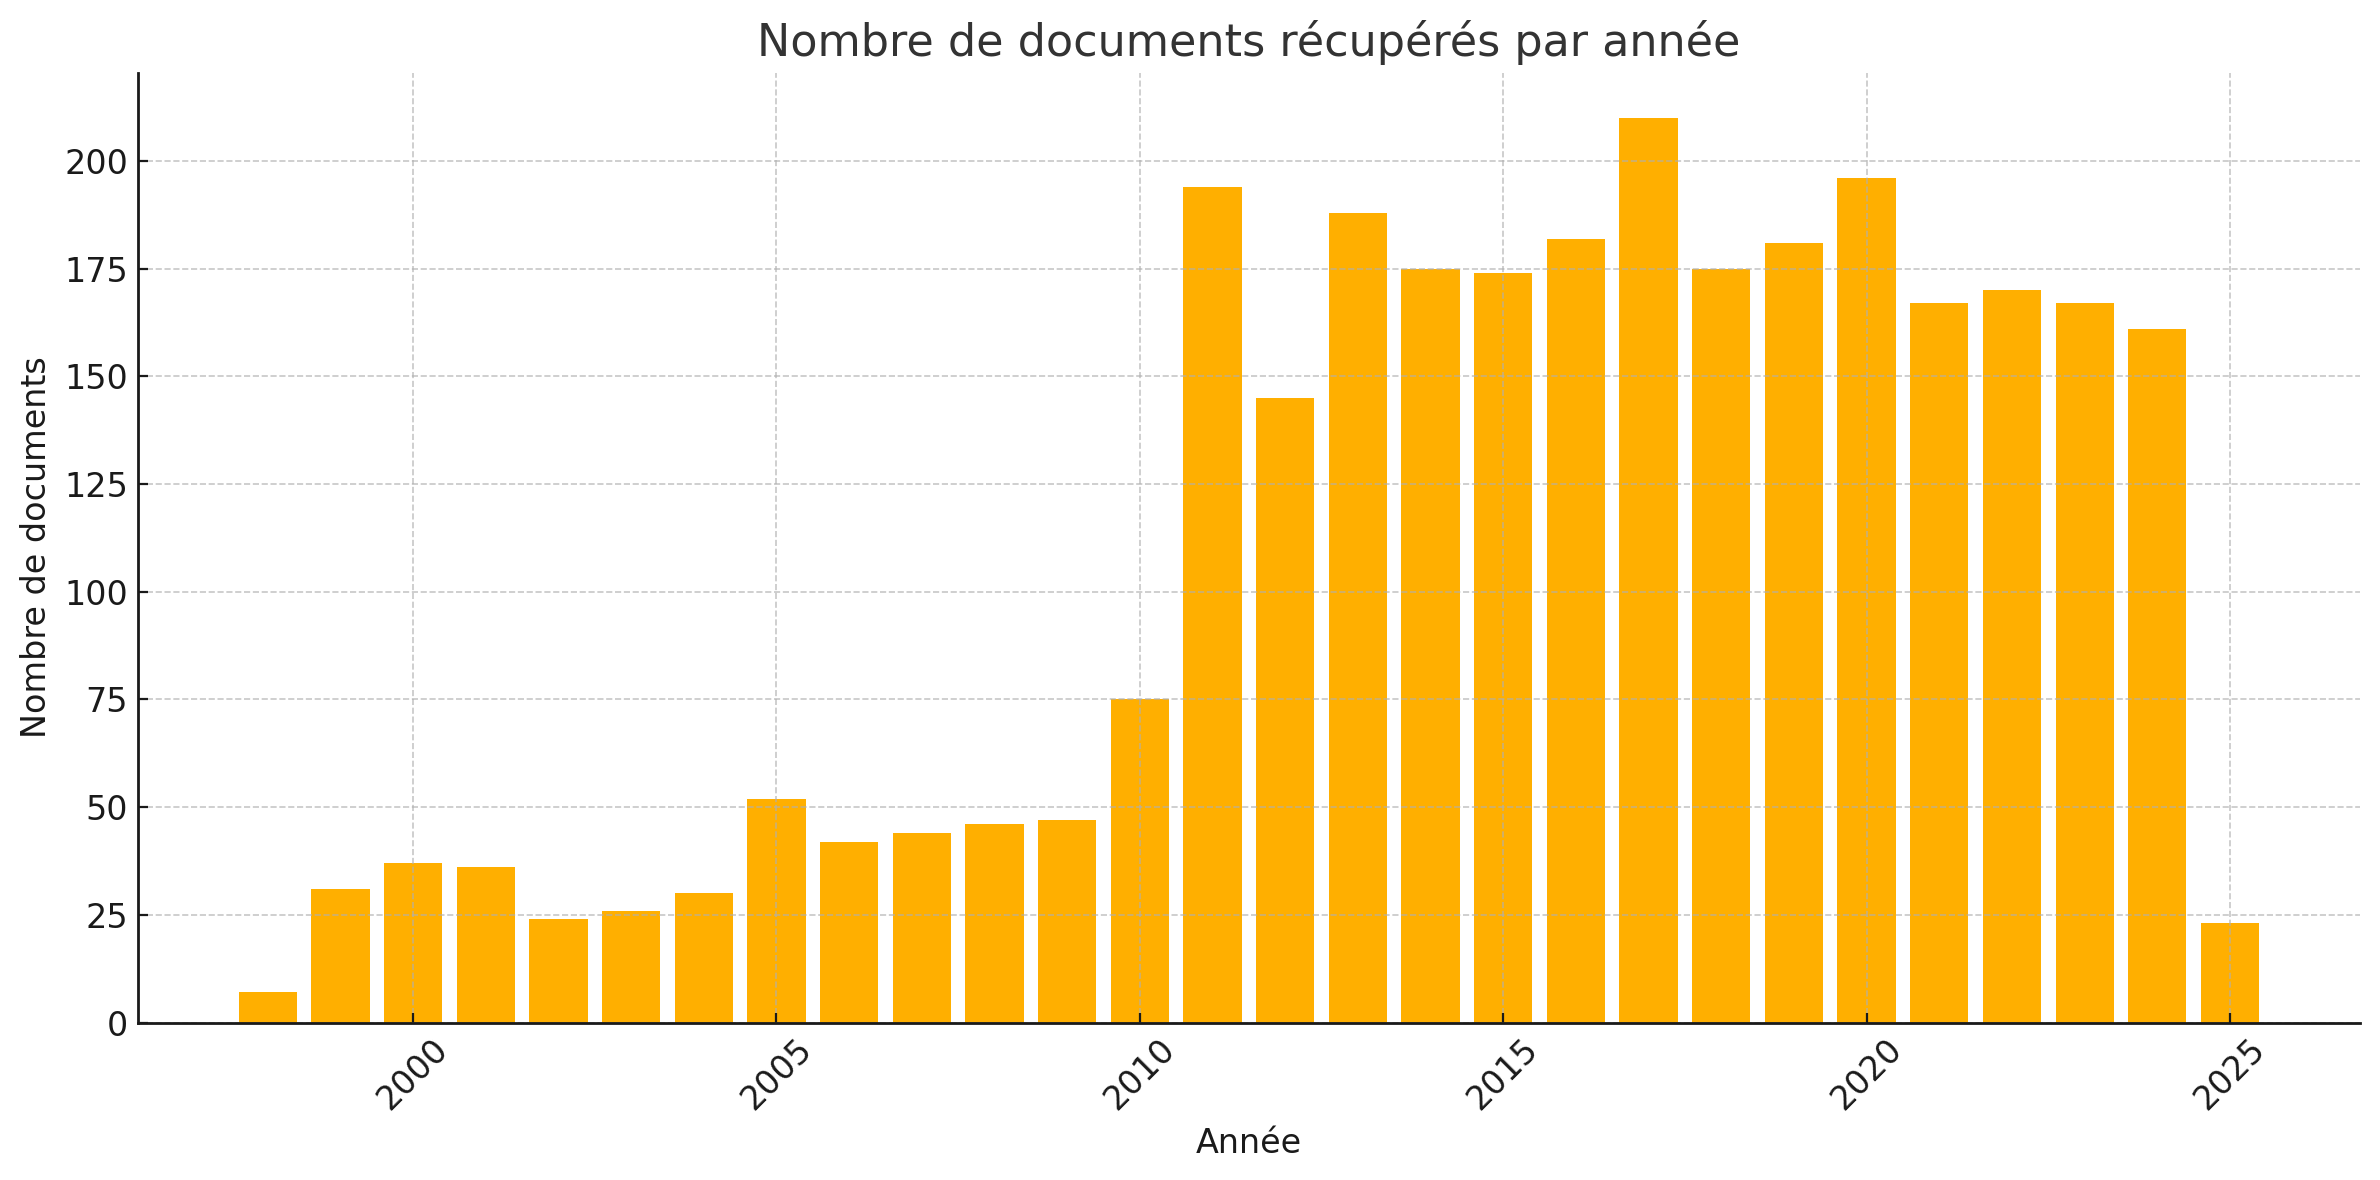
\includegraphics[width=0.9\linewidth]{images/docs_par_annee.png}
    \caption{Nombre de discours et communiqués publiés par la BCE par année (2005–2024)}
    \label{fig:nb_docs_par_annee}
\end{figure}

Il est possible de repérer visuellement plusieurs pics d’activité, généralement corrélés à des périodes de tensions financières ou de révisions majeures de l’orientation monétaire. Ces observations confirment que la fréquence et la densité des discours peuvent elles-mêmes constituer des variables d’intérêt dans l’étude du rôle de la Forward Guidance. Elles suggèrent également l’existence de liens potentiels entre l’intensité de la communication monétaire et les épisodes de stress financier. Afin d’explorer ces liens de manière plus systématique, il convient désormais d’analyser les données relatives au stress systémique, en s’appuyant sur les sous-composantes du CISS, qui mesurent les tensions observées sur les principaux segments des marchés financiers.


\subsection{Données de stress systémique : CISS et sous-composantes}

L'évolution des sous-indicateurs de stress des trois principaux segments financiers : le marché monétaire, le marché des actions et le marché des changes est analysé sous un angle graphique dans la \autoref{fig:graphindicateurs} puis par rapport aux statistiques descriptives dans le \autoref{fig:statsdescriptives}.

\begin{figure}[H]
    \centering
    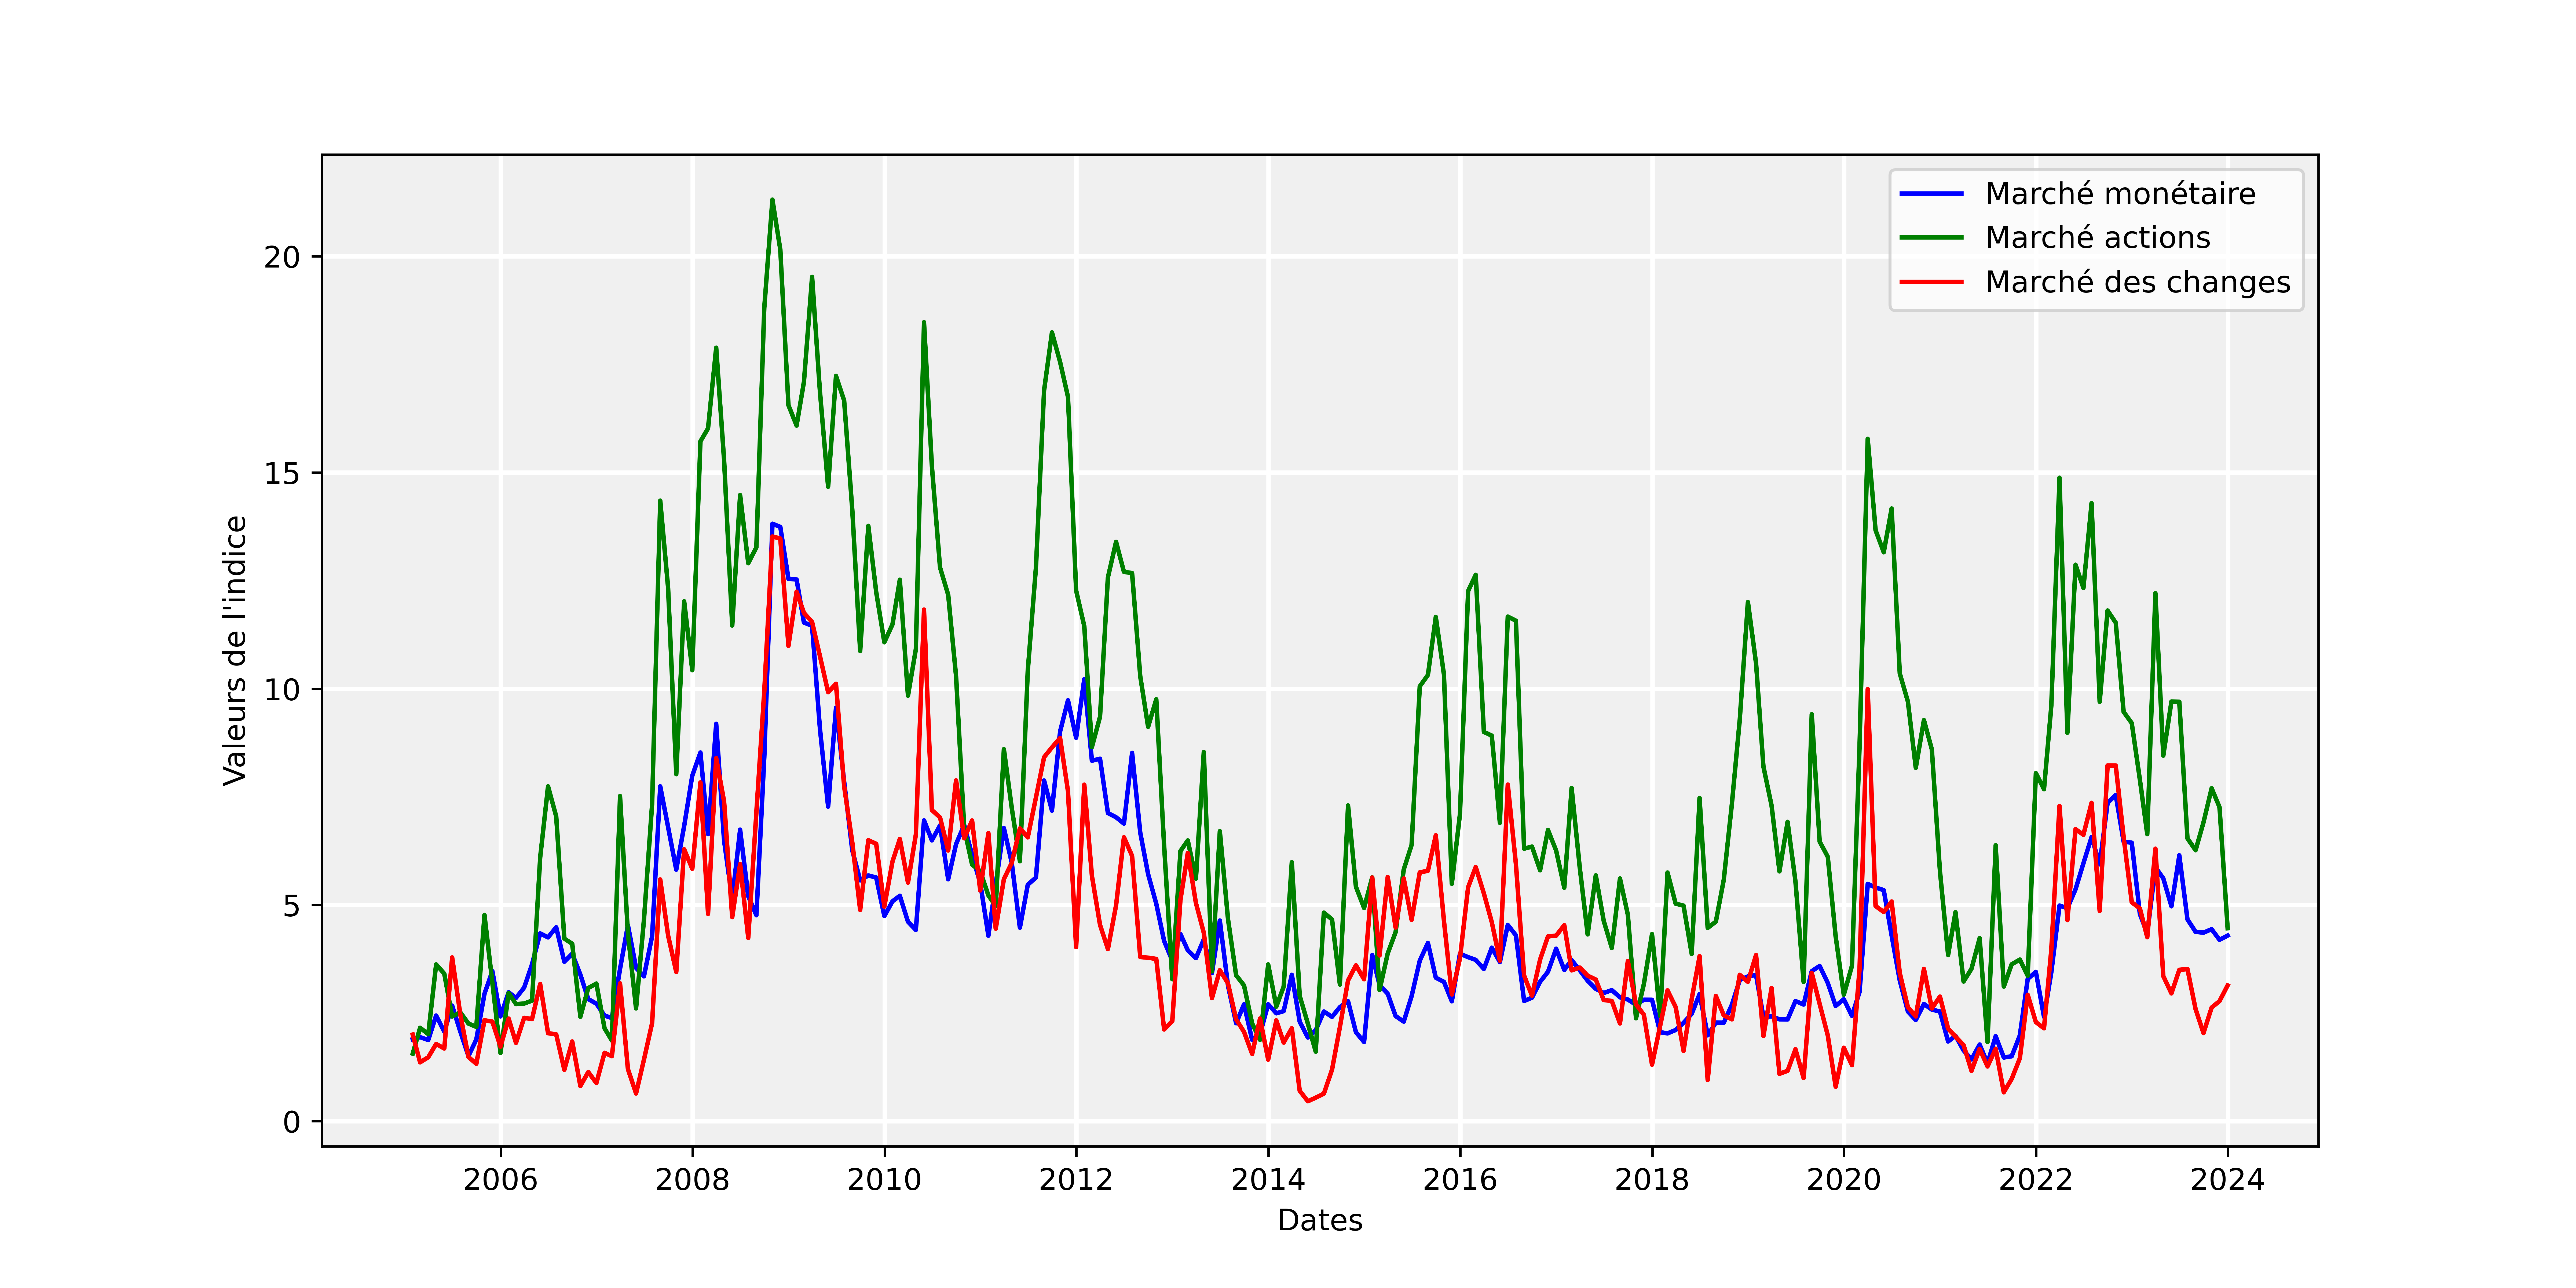
\includegraphics[width=1\linewidth]{images/sous_indicateurs_stress.png}
    \caption{Sous-indicateurs de stress entre janvier 2005 et décembre 2024.}
    \label{fig:graphindicateurs}
\end{figure}

Le graphique montre l'évolution des sous-indicateurs de stress des trois principaux segments financiers (marché monétaire, marché des actions, et marché des changes) entre janvier 2005 et décembre 2024. Chaque indicateur est représenté par une courbe distincte : le marché monétaire est en bleu, le marché des actions en vert, et le marché des changes en rouge.\\

Le marché des actions montre la plus grande volatilité parmi les trois indicateurs. À plusieurs reprises, notamment entre 2008 et 2012 ainsi que vers 2020, des pics marqués, correspondant à des périodes de forte tension sur ce marché. Le stress sur le marché des actions est particulièrement élevé lors des crises financières, comme celle de 2008, où le graphique montre une nette augmentation du stress. Après cette période de crise, le stress sur le marché des actions diminue progressivement, bien que des pics sporadiques apparaissent, notamment en 2020, ce qui pourrait être attribué à la crise liée à la pandémie de COVID-19. En général, la courbe verte représente des variations assez brusques, ce qui reflète la nature plus volatile du marché des actions, particulièrement sensible aux événements macroéconomiques et aux changements dans les conditions du marché mondial.

\begin{figure}[H]
    \centering
    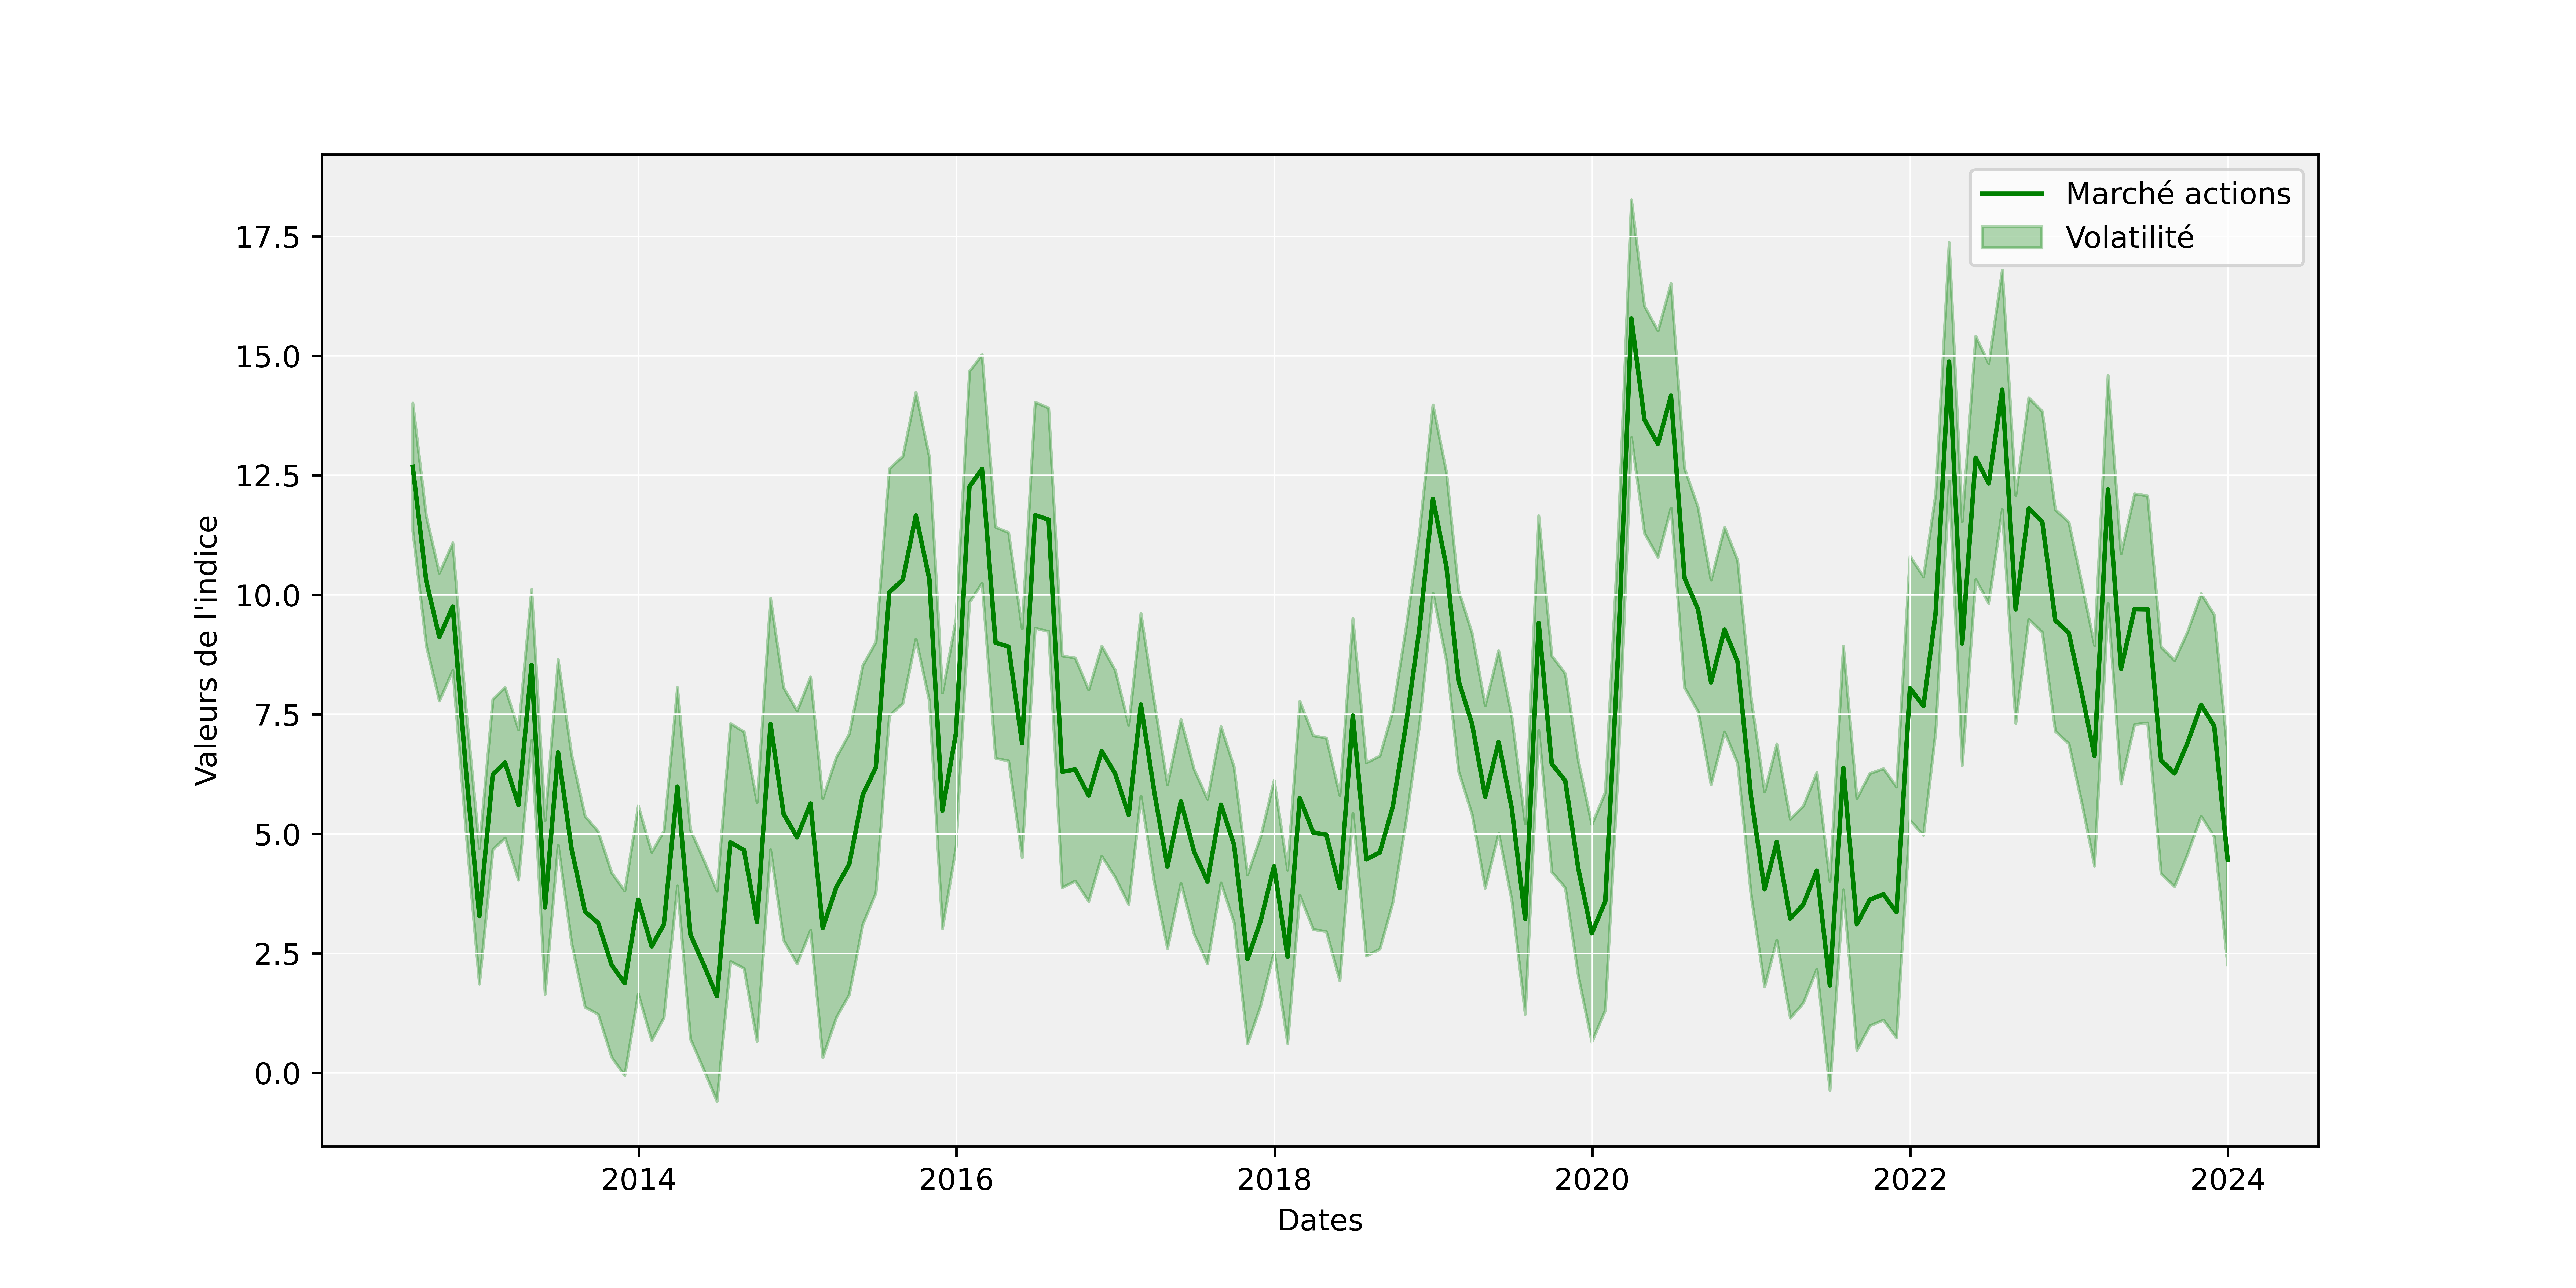
\includegraphics[width=1\linewidth]{images/sous_indicateurs_equity_stress_equity.png}
    \caption{Stress sur le marché actions et volatilité associée entre janvier 2005 et décembre 2024.}
    \label{fig:enter-label}
\end{figure}

La volatilité observée sur le marché des actions suggère que les investisseurs réagissent fortement aux événements qui affectent la confiance dans les entreprises et l’économie en général. Les pics de volatilité élevés, particulièrement en 2008 et 2020, indiquent que les actions subissent des ajustements massifs des portefeuilles des investisseurs, souvent en raison de ventes paniquées ou de changements rapides dans les perspectives économiques.\\

En ce qui concerne le marché monétaire, cela montre des variations plus modérées par rapport aux autres marchés. Bien qu’il y ait des pics de stress, notamment autour des crises financières majeures, les valeurs de l'indicateur restent globalement plus stables. Cela reflète la nature plus régulée et contrôlée du marché monétaire, où les banques centrales interviennent régulièrement pour stabiliser les conditions de liquidité. Il est possible d'observer des pics importants autour de 2008 et un autre vers 2012, correspondant à la crise de la dette souveraine en Europe, ainsi que de légères hausses durant d'autres périodes de tension comme la crise de 2020. Cependant, contrairement au marché des actions, le marché monétaire retourne rapidement à des niveaux de stress plus bas après ces périodes de tension. Cela montre une capacité de stabilisation plus rapide dans ce segment du marché.

\begin{figure}[H]
    \centering
    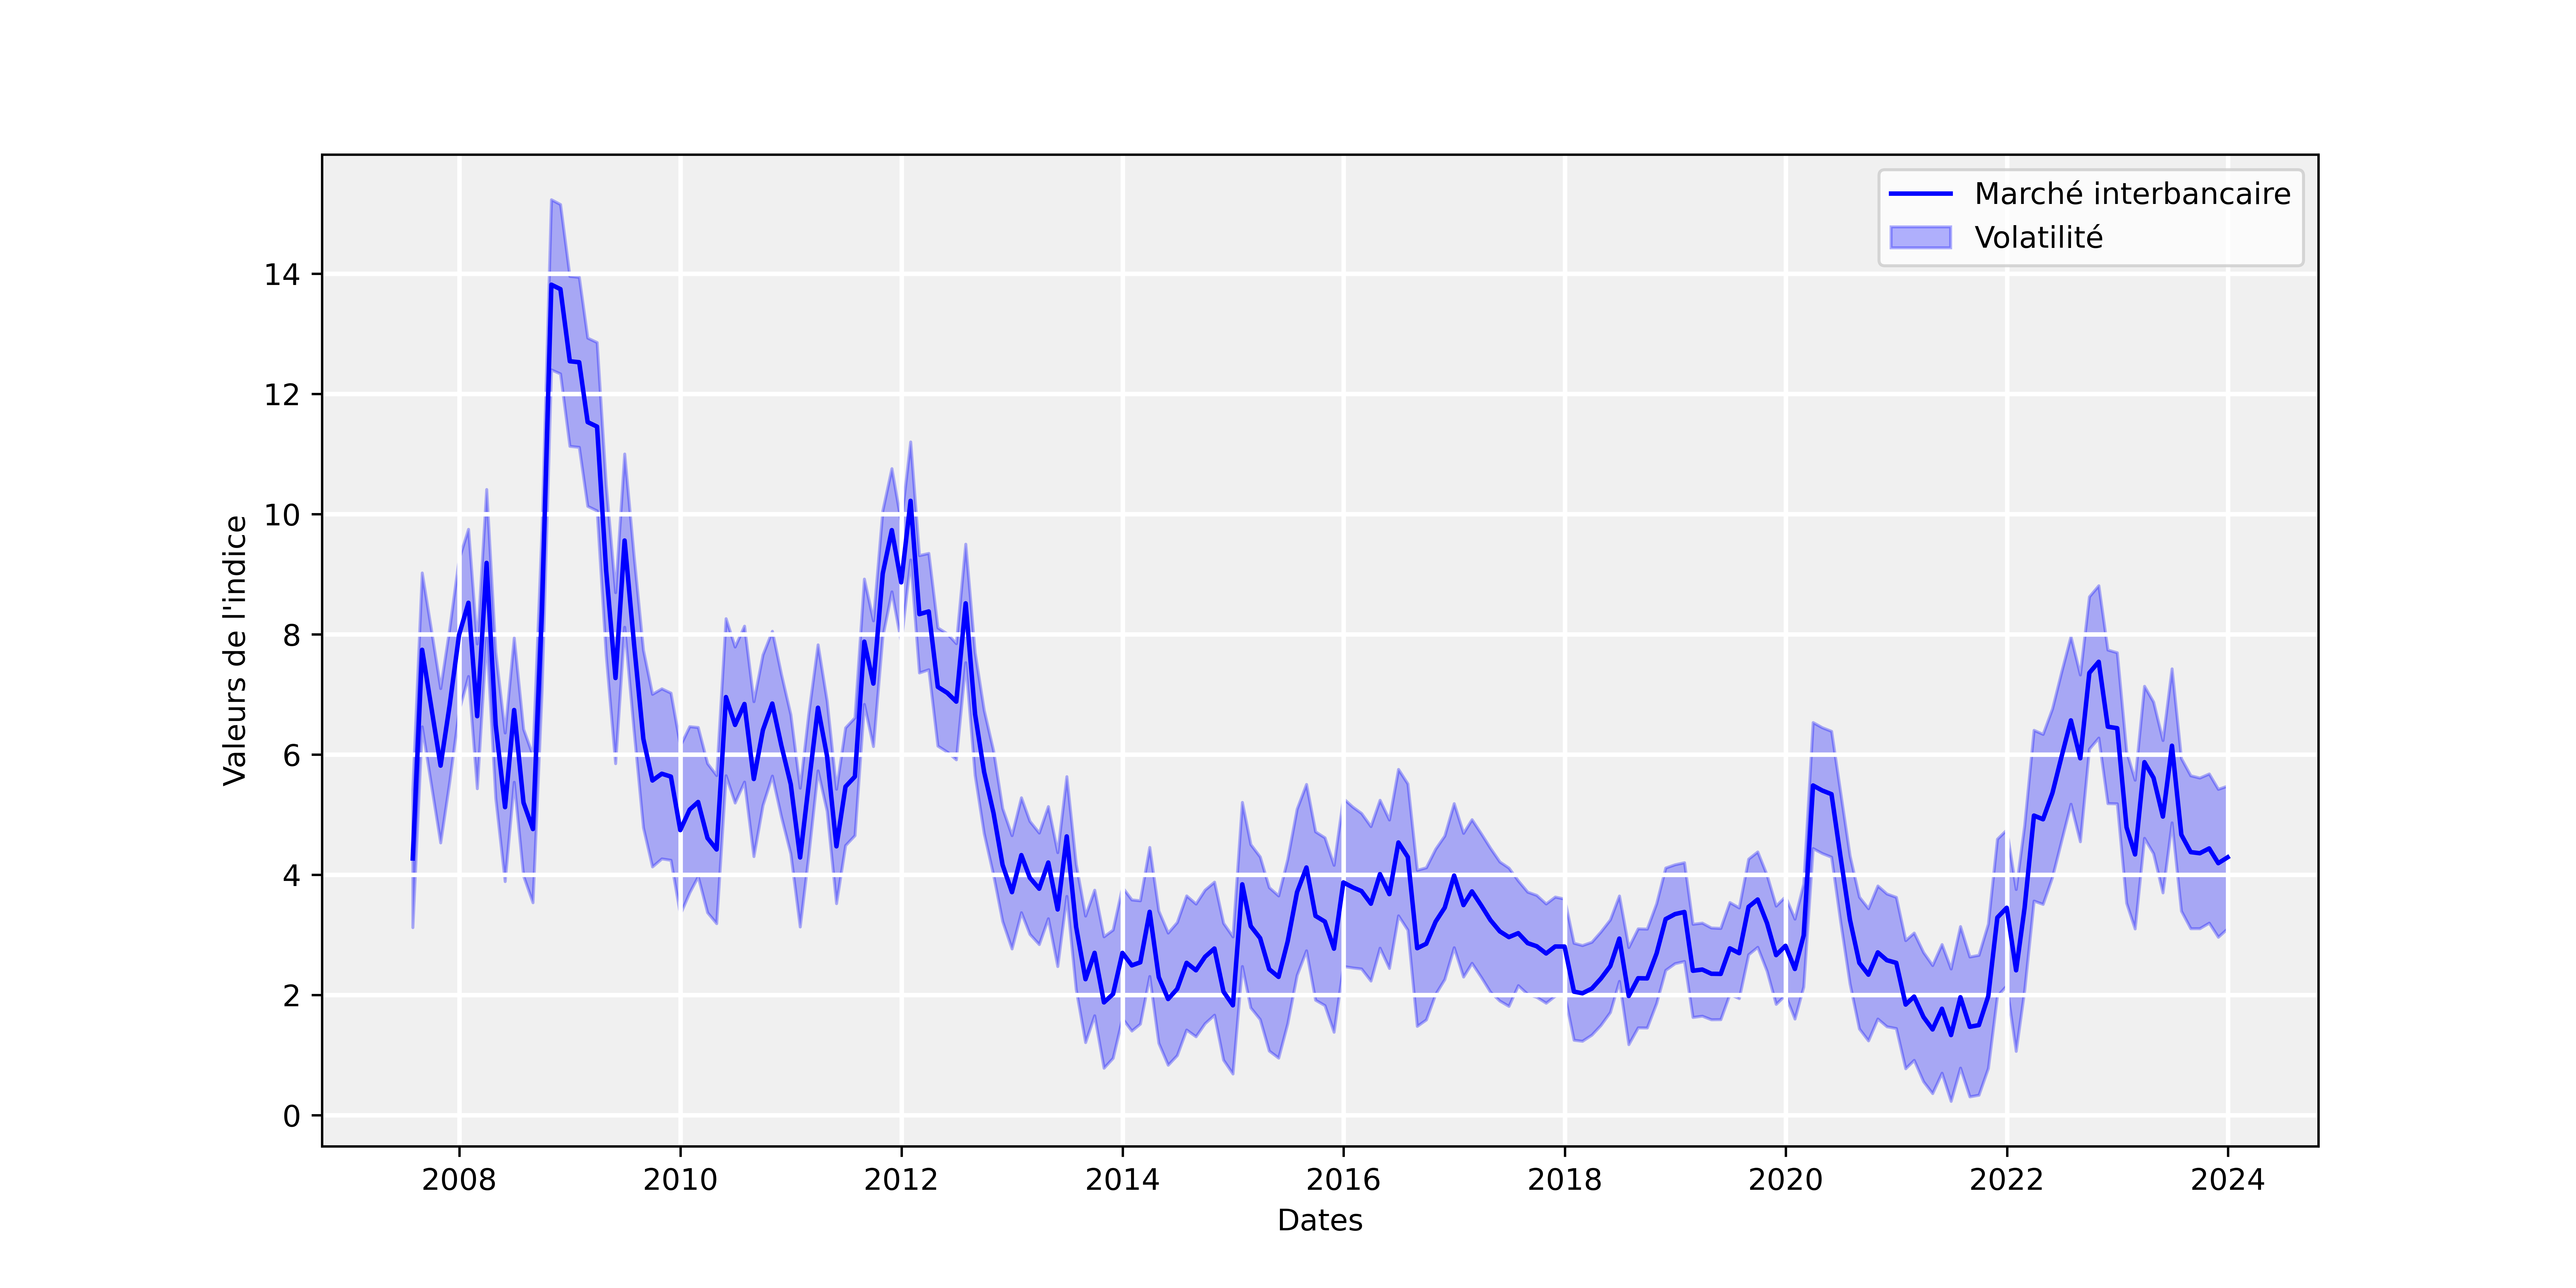
\includegraphics[width=1\linewidth]{images/sous_indicateurs_stress_imm.png}
    \caption{Stress sur le marché monétaire et volatilité associée entre janvier 2005 et décembre 2024.}
    \label{fig:enter-label}
\end{figure}

La volatilité modérée associée au stress sur le marché monétaire, par rapport au marché des actions, est en partie due à la capacité des banques centrales à stabiliser ce marché via leurs outils de politique monétaire. Les pics de volatilité, en particulier en 2008 et 2011, sont le reflet des périodes où les banques hésitent à se prêter mutuellement, indiquant un risque accru de crise de liquidité. Cependant, après les interventions des régulateurs, la volatilité diminue rapidement, témoignant de la résilience de ce marché.\\

Enfin, le marché des changes est globalement le moins stressé parmi les trois segments, comme en témoignent les niveaux relativement bas de la courbe rouge. Cependant, ce marché montre également des épisodes de stress ponctuels, en particulier autour de 2008 et 2010-2012, ainsi que quelques augmentations notables dans les années plus récentes (vers 2020). La nature décentralisée et liquide du marché des changes lui permet de mieux absorber les chocs, bien que des périodes de forte volatilité, notamment causées par les fluctuations des taux de change et les crises monétaires, entraînent des pics soudains. Le stress sur ce marché semble être plus transitoire et moins soutenu que sur le marché des actions, où les tensions persistent souvent sur une plus longue période.

\begin{figure}[H]
    \centering
    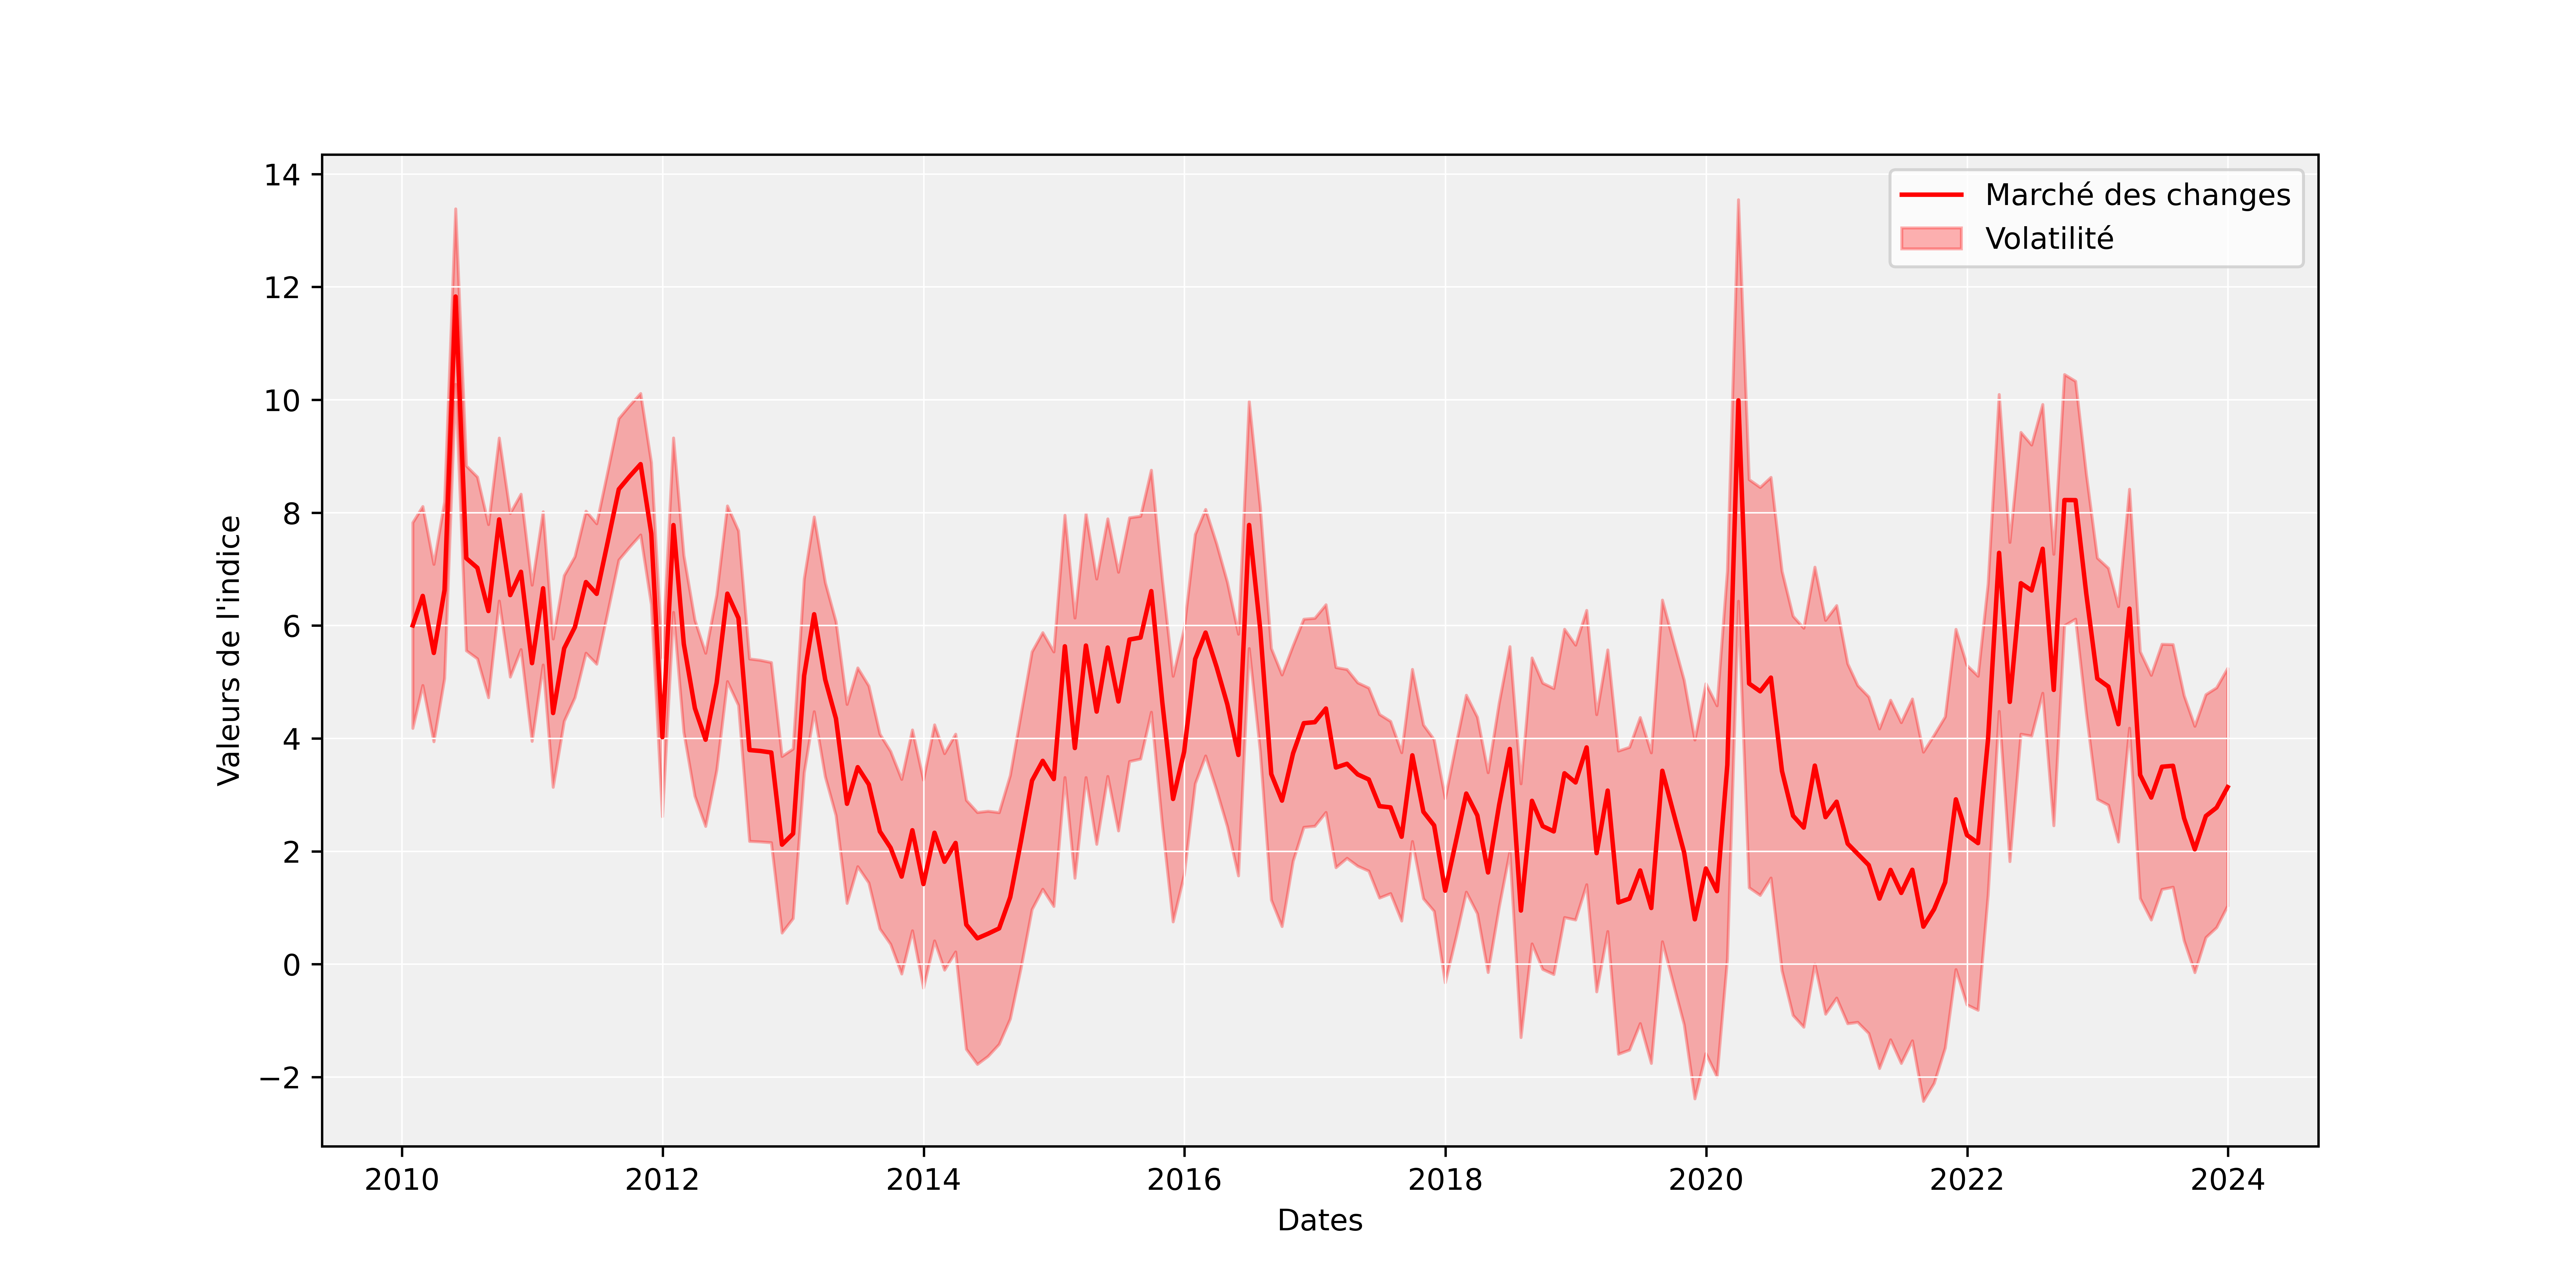
\includegraphics[width=1\linewidth]{images/sous_indicateurs_forex_stress_forex.png}
    \caption{Stress sur le marché des changes et volatilité associée entre janvier 2005 et décembre 2024.}
    \label{fig:enter-label}
\end{figure}

La volatilité, qui accompagne les hausses de stress, est particulièrement importante autour de ces périodes. Les fluctuations observées en 2020 peuvent être attribuées aux mouvements des taux de change lors de la pandémie, ainsi qu'à la réponse des banques centrales à travers des ajustements des taux d'intérêt et des mesures non conventionnelles. Cependant, même si des périodes de stress apparaissent, le marché des changes tend à revenir à des niveaux de stress modérés sur le long terme, reflétant sa capacité à absorber les chocs grâce à sa liquidité élevée et à son caractère global.\\

En somme, l'interconnexion entre ces trois indicateurs de stress est bien visible. Lors des grandes crises financières, comme celle de 2008, on observe des pics simultanés dans les trois indicateurs, ce qui reflète un stress systémique à travers plusieurs segments financiers. Cependant, chaque marché semble réagir différemment en fonction de sa structure et de sa régulation. Le marché des actions tend à subir des chocs plus fréquents et plus sévères, tandis que le marché des changes montre une capacité à absorber les chocs avec des variations moins marquées. Le marché monétaire, quant à lui, présente une stabilité relative, malgré des tensions durant les périodes de crise.\\

Cette analyse démontre l'importance de surveiller l'évolution simultanée des sous-indicateurs de stress pour comprendre comment les tensions dans un segment peuvent se propager aux autres, exacerbant ainsi les crises financières. Après avoir effectué une analyse graphique des sous-indicateurs de stress pour les trois principaux segments financiers, l'analyse des statistiques descriptives va être menée. Cette approche permettra de mieux comprendre la distribution et les caractéristiques des différents indicateurs de stress en quantifiant leur tendance centrale, leur dispersion.

\begin{table}[H]
    \centering
    \sffamily
    \scalebox{0.9}{\begin{tabular}{lccccccc}
        \toprule
        \textbf{Indicateurs} & \textbf{Moyenne} & \textbf{Médiane} & \textbf{Maximum} & \textbf{Minimum} & \textbf{Écart-type} & \textbf{Skewness} & \textbf{Kurtosis} \\
        \midrule
        IMM      & 4.39  & 3.68  & 13.82  & 1.33  & 2.38  & 1.45  & 5.35  \\
        FOREX    & 4.19  & 3.52  & 13.52  & 0.46  & 2.65  & 1.09  & 4.07  \\
        EQUITY   & 8.02  & 6.91  & 21.31  & 1.56  & 4.56  & 0.68  & 2.64  \\
        \bottomrule
\end{tabular}
}
    \caption{Statistiques descriptives.}
    \label{fig:statsdescriptives}
\end{table}

L'analyse des moyennes montre que l'indicateur de stress sur le marché des actions  présente la valeur moyenne la plus élevée avec 8.02, suivie par les marchés interbancaire et des changes avec des moyennes respectives de 4.39 et 4.19. Cela suggère que, dans l'ensemble, le marché des actions tend à subir un stress plus important que les marchés des changes et interbancaire. En observant les valeurs médianes, il est possible de voir que le marché des actions affiche également la valeur médiane la plus élevée (6.91), ce qui renforce l'idée que ce marché est plus fréquemment sujet à des périodes de stress élevé. Les marchés interbancaire et des changes ont des valeurs médianes plus proches de leur moyenne, respectivement à 3.68 et 3.52, ce qui indique une distribution des données plus symétrique, bien que des périodes de stress aigu existent.\\

Les valeurs maximales et minimales montrent que marché des actions a connu des pics de stress beaucoup plus élevés, avec une valeur maximale de 21.31, contre 13.82 pour l'IMM et 13.52 pour le FOREX. De plus, les valeurs minimales montrent que le marché des changes a subi des périodes de stress très faibles avec une valeur minimale de 0.46, beaucoup plus basse que celles observées sur les marchés interbancaire (1.33) et des actions (1.56). Cela suggère que le marché des changes est potentiellement plus volatil avec des périodes de très faible stress ainsi que des pics de stress relativement élevés.

\newpage

L'écart-type permet de mesurer la dispersion des données autour de la moyenne, il est aussi une mesure de la volatilité. L'indicateur de stress du marché des actions présente une dispersion plus large (4.56), indiquant une plus grande volatilité des niveaux de stress par rapport aux autres marchés. Le FOREX montre également une volatilité non négligeable avec un écart-type de 2.65, tandis que l'IMM affiche la plus faible volatilité avec 2.38.\\

En examinant les coefficients d'asymétrie, tous les indicateurs présentent une asymétrie positive, ce qui signifie que les périodes de stress extrême sont plus fréquentes du côté des valeurs élevées. Le marché interbancaire présente la plus forte asymétrie (1.45), ce qui indique que ce marché connaît des épisodes de stress élevé relativement rares mais intenses. Le FOREX est également assez asymétrique avec une valeur de 1.09, tandis que le marché des actions présente une asymétrie plus modérée avec un coefficient de 0.68. Enfin, les coefficients de kurtosis montrent des informations sur la forme de la distribution des stress. Le marché interbancaire présente une kurtosis de 5.35, ce qui indique une distribution leptokurtique, caractérisée par des extrêmes plus fréquents et des périodes de stress aigu prononcées. Le FOREX affiche également une kurtosis élevée à 4.07, tandis que le marché des actions présente une distribution plus aplatie (2.64), indiquant une distribution plus proche de la normale.\\

Cela montre donc que le marché des actions tend à subir un stress plus élevé et plus volatil que les marchés des changes et interbancaire. Cependant, les périodes de stress intense sur le marché interbancaire se caractérisent par des épisodes plus rares mais plus extrêmes, comme le montrent ses valeurs de skewness et de kurtosis.

\subsection{Alignement temporel et granularité}

Afin de permettre une analyse cohérente entre les discours de la BCE et les indicateurs de stress financier, un alignement temporel des séries de données a été mis en œuvre. Les deux ensembles (textuel et quantitatif) ont été synchronisés à une fréquence hebdomadaire, considérée comme le compromis optimal dans le cadre de l’analyse de la politique monétaire et de l’impact de la Forward Guidance. Cette granularité permet de capturer des dynamiques suffisamment fines sans être affectées par le bruit de haute fréquence, tout en assurant une représentation temporelle compatible avec le rythme des communications institutionnelles et les évolutions des marchés financiers.\\

Pour chaque date hebdomadaire correspondant à une observation du CISS (de janvier 2005 à décembre 2024), un discours de la BCE a été associé selon une règle précise : si plusieurs discours étaient disponibles durant la semaine, celui correspondant exactement à la date d’observation du CISS était privilégié. En l’absence de discours à cette date, le discours le plus proche dans le passé (mais jamais postérieur) a été sélectionné. Ce choix méthodologique garantit une stricte antériorité du signal discursif par rapport à l’indicateur de stress, condition nécessaire pour préserver la validité causale dans les analyses ultérieures. Du côté des données quantitatives, les sous-indicateurs de stress extraits du CISS sont directement exploitables à fréquence hebdomadaire, sans nécessité d’agrégation supplémentaire. L’ensemble du dispositif aboutit ainsi à la constitution de couples temporels $(X_t, y_t)$, où $X_t$ désigne le discours institutionnel sélectionné à la date $t$ et $y_t$ la valeur du stress systémique observée cette même semaine. Cette construction permet une mise en correspondance rigoureuse des données textuelles et numériques, indispensable pour évaluer de manière crédible l’impact différé de la Forward Guidance sur la stabilité financière.\\

En définitive, l’analyse statistique exploratoire menée a permis de caractériser en détail les deux piliers empiriques du présent mémoire : d’une part, la structure et la temporalité des discours officiels de la Banque Centrale Européenne ; d’autre part, la dynamique et la distribution des tensions financières captées par les sous-indicateurs du CISS. La mise en lumière des régularités statistiques propres à chaque segment constitue une étape préparatoire à la modélisation intégrée. Elle justifie notamment le recours à des approches capables de capturer simultanément les dimensions sémantiques de la communication monétaire et les réponses structurelles des marchés. C’est dans cette perspective que s’ouvre désormais le paragraphe suivant, consacrée à la construction d’un indicateur directionnel de FG. À partir du corpus textuel analysé, il s’agira de quantifier, à l’aide de modèles de langage avancés, la tonalité implicite des discours de la BCE sur un axe allant de l’accommodant au restrictif. Cette mesure permettra d’intégrer la dimension sémantique de la politique monétaire dans un cadre de modélisation dynamique du stress systémique.

\section{Construction de l’indicateur de Forward Guidance}

Précédemment, il a été posé les fondations empiriques de ce travail, en décrivant la structure des données textuelles issues des publications de la BCE ainsi que les dynamiques observées des tensions financières à travers les composantes du CISS. Cette double caractérisation met en évidence la nécessité de relier de manière formalisée le contenu sémantique de la communication monétaire aux évolutions du stress systémique. Dans cette optique, ce paragraphe introduit une méthodologie de construction d’un indicateur directionnel de FG, fondé sur des techniques d’apprentissage profond appliquées au traitement automatique du langage. L’objectif est de transformer des discours non structurés en une variable continue, reflétant le ton monétaire implicite véhiculé par la BCE au fil du temps. L’approche adoptée combine la richesse contextuelle des modèles transformeurs de dernière génération avec la simplicité interprétative d’un axe latent construit à partir d’exemples de référence générés par LLM. Trois LLM ont été choisis : Llama 3, Mistral 7B et Gemini. Chaque phrase $x$ est d’abord encodée en un vecteur dense de dimension $d$ grâce à ModernBERT, Mamba, Mamba-2 et Llamba. Elle est ensuite projetée sur un vecteur directionnel $\hat V$ obtenu par différence entre phrases canoniquement expansives et restrictives. Le coefficient de projection brut, qui reflète la proximité sémantique de $x$ avec les déclarations expansives, est finalement centré et réduit à l’aide des mêmes phrases d’ancrage afin de produire un score normalisé $z_x$.  Contrairement à une classification binaire, cette
construction fournit un indice continu qui capture les nuances de la communication de la BCE, tant au niveau intra-phrase qu’au niveau agrégé, sans nécessiter de supervision exhaustive. Il est ainsi détaillé successivement le processus d’encodage des textes, la modélisation de la direction sémantique, le calcul du score directionnel, et enfin, l’évaluation comparative des différents encodeurs via une analyse de régression. L’objectif est de sélectionner l’indicateur le plus informatif pour expliquer les fluctuations du stress systémique, dans la perspective d’une modélisation.

\newpage

\subsection{Encodage des textes et modèles de langage}

Afin de quantifier la tonalité de ces communications, chaque document du corpus a été encodé en vecteur numérique à l’aide de modèles de langage pré-entraînés. Trois modèles différents ont été retenus pour générer ces représentations sémantiques : ModernBERT, Mamba et Llamba. ModernBERT est un modèle de type BERT « modernisé » (intégrant des améliorations récentes des transformeurs, comme présenté dans le paragraphe précédent) offrant des embeddings contextuels bidirectionnels. Mamba correspond à une architecture alternative de nouvelle génération réputée pour capturer efficacement les dépendances longues. Enfin, Llamba est dérivé d’un large modèle de langage de la famille LLaMA, exploité ici pour produire des embeddings textuels.\\

Pour chaque document, le texte complet est passé dans chacun de ces modèles afin d’en extraire une représentation vectorielle dense. Concrètement, il est utilisé les représentations du dernier niveau de chaque modèle et appliqué une opération de mean pooling c’est-à-dire une moyenne des vecteurs de tous les tokens du document afin d’obtenir un unique vecteur par document. Mathématiquement, soit un document constitué de $L$ tokens, auxquels le modèle associe une matrice d’embeddings :

\begin{equation}
\mathbf{H} = \begin{bmatrix}
h_1^\top \\
h_2^\top \\
\vdots \\
h_L^\top
\end{bmatrix} \in \mathbb{R}^{L \times d}
\quad \text{où } h_i \in \mathbb{R}^d
\end{equation}

L’opération de mean pooling consiste à réduire cette matrice $L \times d$ en un vecteur unique $\bar{h} \in \mathbb{R}^d$ selon :

\begin{equation}
\bar{h} = \frac{1}{L} \sum_{i=1}^L h_i
\end{equation}

Cette réduction de dimension se fait donc uniquement sur l’axe des tokens (longueur du document $L$), tout en conservant la dimension sémantique $d$ du modèle. Le passage de $\mathbb{R}^{L \times d}$ à $\mathbb{R}^d$ permet d'obtenir une représentation compacte, fixe et exploitable par la suite pour des tâches telles que la classification, la projection directionnelle ou la régression.\\

La dimension $d$ de ces vecteurs dépend du modèle (par exemple, ~768 composantes pour ModernBERT base, davantage pour des modèles plus volumineux), mais dans chaque cas il s’agit de vecteurs dans un espace sémantique de haute dimension. Chaque document est ainsi associé à un vecteur numérique résumé de sa teneur textuelle.\\

Ainsi, chaque document est désormais représenté par un vecteur dense dans un espace sémantique de grande dimension, propre à chaque modèle de langage. Ces embeddings constituent une base vectorielle unifiée permettant d’analyser les discours de la BCE sous un angle quantitatif. Toutefois, pour que cette représentation prenne sens dans le cadre spécifique de la Forward Guidance, il convient d’y superposer une structure directionnelle pertinente. C’est l’objet suivant, qui vise à définir un axe sémantique latent capturant l’opposition entre tonalités monétaires expansives et restrictives. Ce vecteur directionnel permettra de projeter chaque document dans une dimension interprétable, en traduisant sa proximité avec les discours typiques d’assouplissement ou de resserrement.

\subsection{Direction sémantique de restrictive à expansive}

L’élaboration de l’indicateur directionnel de Forward Guidance repose sur la modélisation d’un axe sémantique latent dans l’espace des représentations vectorielles issues d’un modèle de langage. Cet axe vise à capturer la dimension sémantique dominante opposant les discours de type dovish (orientés vers un assouplissement monétaire) à ceux de type hawkish (orientés vers un resserrement monétaire). Contrairement aux approches traditionnelles où les phrases d’ancrage sont sélectionnées manuellement, une génération automatisée a été adoptée dans cette étude. Plus précisément, les phrases d’ancrage représentant les deux extrémités du spectre sémantique sont générées à l’aide de trois LLM, en l’occurrence LLaMA-3 Mistral-7B et Gemini, via des instructions construites pour produire des énoncés caractérisant des tonalités de politique monétaire fortement expansionniste ou fortement restrictive.\\

Les prompts fournis au modèle sont calibrés pour produire des phrases dans le style des déclarations de la BCE, mais contenant explicitement un biais accommodant ou restrictif. Des contraintes syntaxiques et lexicales ont été imposées afin de garantir la clarté des exemples générés. Une validation humaine a ensuite été réalisée afin de s’assurer de la pertinence sémantique des sorties du modèle.

Par exemple, les phrases suivantes ont été retenues :
\begin{itemize}
\item Tonalité expansionniste : « La politique monétaire restera accommodante aussi longtemps que nécessaire pour soutenir la reprise. »
\item Tonalité restrictive : « Le resserrement de la politique monétaire est indispensable pour contenir durablement les tensions inflationnistes. »
\end{itemize}

Ces phrases générées ont été encodées à l’aide des différents encodeurs retenus, afin d’obtenir des représentations vectorielles denses dans un espace sémantique de dimension $d$. Soient $\{ h_1^{+}, \ldots, h_N^{+} \} \subset \mathbb{R}^d$ les vecteurs associés aux phrases expansionnistes, et $\{ h_1^{-}, \ldots, h_M^{-} \} \subset \mathbb{R}^d$ ceux des phrases restrictives. Les centroïdes sémantiques des deux classes sont calculés par moyenne vectorielle simple :

\begin{equation}
\mu^{+} = \frac{1}{N} \sum_{i=1}^N h_i^{+}, \qquad \mu^{-} = \frac{1}{M} \sum_{j=1}^M h_j^{-}
\end{equation}

La direction sémantique latente, notée $\vec{d} \in \mathbb{R}^d$, est alors définie comme :

\begin{equation}
\vec{d} = \mu^{-} - \mu^{+}
\end{equation}

Ce vecteur $\vec{d}$ représente une dimension sémantique orientée, capturant la transition graduelle entre les deux pôles discursifs. Il définit un axe dans l’espace latent des embeddings, le long duquel les discours peuvent être projetés pour en regarder leur tonalité relative.\\

La construction de cette direction sémantique latente permet ainsi de doter l’espace des représentations vectorielles d’une structure interprétable, où chaque point peut être situé relativement à un axe allant des déclarations les plus accommodantes aux plus restrictives. Cette orientation dans l’espace sémantique fournit le fondement nécessaire à la quantification systématique de la tonalité des discours. Il s’agit à présent d’exploiter cette direction pour attribuer à chaque document un score de tonalité, c’est-à-dire une mesure numérique reflétant son positionnement relatif sur l’axe expansionniste–restrictif.

\subsection{Score de tonalité}

La direction sémantique $\vec{d} \in \mathbb{R}^d$, construite à partir des centroïdes de phrases d’ancrage générées par les LLM, définit une dimension latente pertinente dans l’espace des représentations vectorielles. Cette direction est interprétée comme un axe sémantique structurant la communication monétaire selon une opposition entre deux régimes discursifs : expansionniste (ou accommodant) et restrictif (ou resserré). Une fois cette direction construite, elle permet d’attribuer à chaque document de politique monétaire un score directionnel de Forward Guidance, lequel quantifie la position du discours sur l’axe défini. Le passage d’un texte non structuré à un tel score s’opère en plusieurs étapes, qui sont détaillées ci-après.\\

La position du document par rapport à la direction sémantique $\vec{d}$ est ensuite déterminée par la projection directionnelle du vecteur $h_x$ sur $\vec{d}$. Cette projection n’est pas réalisée de manière orthogonale, mais plutôt en mesurant l’alignement directionnel, évalué par la similarité cosinus entre les deux vecteurs. Ce choix permet d’ignorer l’échelle absolue de $h_x$ et de se concentrer sur son orientation relative. Le score brut de FG est alors défini comme :

\begin{equation}
s(x) = \cos(\theta_x) = \frac{\langle h_x, \vec{d} \rangle}{\|h_x\| \cdot \|\vec{d}\|}
\end{equation}

où $\theta_x$ est l’angle entre le vecteur du document et la direction sémantique.\\

Ce score $s(x) \in [-1, 1]$ permet une interprétation directe :

\begin{itemize}
    \item Une valeur $s(x) \approx 1$ indique un alignement fort avec le pôle restrictif, caractérisant un discours orienté vers un resserrement monétaire.
    \item Une valeur $s(x) \approx -1$ traduit une proximité sémantique avec le pôle expansionniste, typique d’un ton accommodant.
    \item Une valeur proche de zéro implique un positionnement neutre ou ambigu sur l’axe directionnel.
\end{itemize}

Bien que le score $s(x)$ soit déjà compris dans un intervalle borné, une standardisation est appliquée pour assurer une comparabilité temporelle et faciliter l’interprétation statistique. En effet, la distribution empirique de $s(x)$ peut être centrée sur une valeur non nulle, et sa dispersion peut varier selon les périodes. Il est donc procédé à un centrage-réduction, définissant un score normalisé $z_x$ :

\begin{equation}
z_x = \frac{s(x) - \mu_s}{\sigma_s}, \quad \text{où } \mu_s = \frac{1}{T} \sum_{t=1}^T s(x_t), \quad \sigma_s^2 = \frac{1}{T} \sum_{t=1}^T \left(s(x_t) - \mu_s \right)^2.
\end{equation}

Cette opération garantit que l’espérance empirique de $z_x$ sur l’échantillon est nulle : $\mathbb{E}[z_x] = 0$ et que la variance est unitaire : $\mathbb{V}[z_x] = 1$. Le score $z_x \in \mathbb{R}$ peut alors être interprété comme une déviation standardisée de la tonalité du discours $x$ par rapport à l’ensemble des communications de la période.\\

L’indice directionnel $z_x$, associé à chaque document $x$, constitue un indicateur numérique unidimensionnel de la tonalité de Forward Guidance exprimée dans le discours. Une valeur $z_x > 0$ reflète un discours plus restrictif que la moyenne historique, tandis qu’une valeur $z_x < 0$ indique une communication plus accommodante que la norme. Ce type de mesure permet d'une part de suivre l’évolution temporelle de la posture de la BCE. D'autre part de comparer la tonalité de documents au sein d’une même année ou entre cycles de politique monétaire. Enfin, cela permet d'analyser les ruptures de ton associées à des événements macroéconomiques majeurs. L’utilisation d’un espace latent de grande dimension combiné à une projection vectorielle linéaire permet de quantifier des phénomènes sémantiques jusque-là difficilement mesurables de manière systématique.\\

L’indice $z_x$ ainsi obtenu est conçu pour être utilisé comme variable explicative dans des modèles temporels, en vue d’évaluer l’impact de la tonalité de Forward Guidance sur le stress systémique tel que mesuré par l’indicateur CISS. Il est également possible de dériver des statistiques agrégées (moyennes mobiles, quantiles temporels, chocs sémantiques) pour en dégager des dynamiques structurelles.\\

L’indice directionnel $z_x$ constitue ainsi une mesure continue, standardisée et interprétable de la tonalité des discours de politique monétaire. Il permet de quantifier finement l’orientation de la communication de la BCE, tout en conservant une compatibilité avec les approches économétriques traditionnelles comme les régressions linéaires, modèles VAR ou encore à changements de régime. Sa construction, fondée sur des techniques d’encodage sémantique et une structuration vectorielle explicite, permet une exploitation empirique. Il convient désormais d’évaluer empiriquement la pertinence de cet indicateur, en examinant dans quelle mesure les différentes versions de $z_x$ (issues de plusieurs encodeurs) permettent d’expliquer les variations observées du stress systémique. C’est l’objet du prochain paragraphe, qui s’appuie sur un modèle de régression Ridge pour comparer leur pouvoir explicatif.

\subsection{Évaluation quantitative par régression Ridge}

Plusieurs indicateurs de Forward Guidance ont donc été construits, chacun étant dérivé d’un encodeur différent. Plus précisément, quatre versions alternatives de l’indicateur directionnel $z_x$ ont été générées à partir des représentations produites respectivement par ModernBERT, Mamba, Mamba-2 et Llamba. Chaque encodeur fournit une représentation vectorielle propre à chaque discours, sur la base de laquelle un score de Forward Guidance est calculé par projection dans l’espace latent, comme exposé précédemment. Ces indicateurs sont conceptuellement équivalents, mais diffèrent par la manière dont l’information sémantique est encodée dans l’espace des embeddings.\\

L’objectif est alors de déterminer quel encodeur produit l’indicateur le plus informatif pour l’analyse du stress systémique. Pour ce faire, une analyse de régression supervisée a été mise en place afin de relier chaque version de l’indicateur $z_x^{(m)}$ (où l’exposant $(m) \in \{\text{ModernBERT}, \text{Mamba}, \text{Mamba-2}, \text{Llamba}\}$ identifie l’encodeur utilisé) à une variable cible représentant le niveau du stress systémique, tel que mesuré par le CISS.\\

Le modèle de régression retenu est une régression Ridge, c’est-à-dire une régression linéaire pénalisée par une norme quadratique $\ell_2$. Ce choix méthodologique se justifie par plusieurs considérations :
\begin{itemize}
\item Tout d’abord, la pénalisation quadratique permet de contrôler la variance de l’estimation, en particulier dans un cadre où les signaux extraits sont fortement corrélés temporellement et peuvent contenir du bruit sémantique résiduel.
\item Ensuite, la régularisation assure une meilleure robustesse hors échantillon, ce qui est crucial lorsqu’un score directionnel est utilisé dans un cadre prédictif ou de stress testing.
\item Enfin, l’usage d’une pénalisation $\ell_2$ permet d’opérer une comparaison équitable entre les modèles : en contrôlant la complexité effective des régressions, les performances sont rendues comparables même si les embeddings initiaux diffèrent en structure ou en richesse expressive.
\end{itemize}

La forme fonctionnelle du modèle estimé est la suivante :

\begin{equation}
y_t = \beta_0^{(m)} + \beta_1^{(m)} z_t^{(m)} + \varepsilon_t,
\end{equation}

où :

$y_t$ désigne l’indice de stress systémique à la date $t$, $z_t^{(m)}$ est le score de Forward Guidance associé à l’encodeur $m$, $\beta_0^{(m)}, \beta_1^{(m)}$ sont les paramètres estimés sous pénalisation Ridge et $\varepsilon_t$ est un terme d’erreur gaussien supposé centré et homoscédastique.\\

La qualité explicative de chaque modèle est évaluée au moyen du coefficient de détermination $R^2$, calculé soit sur un jeu de test, soit par validation croisée. Ce coefficient reflète la proportion de la variance du stress systémique qui est expliquée par la variation du score de Forward Guidance :

\begin{equation}
R^2 = 1 - \frac{\sum_{t} \left( y_t - \hat{y}_t^{(m)} \right)^2}{\sum_{t} \left( y_t - \bar{y} \right)^2}.
\end{equation}

Le meilleur encodeur est sélectionné comme celui dont le score directionnel $z_x^{(m)}$ maximise le $R^2$, c’est-à-dire celui dont l’indicateur de Forward Guidance explique le mieux les fluctuations du stress systémique. Ce critère permet de guider le choix du modèle linguistique sous-jacent à la construction de l’indice, en vue d’une utilisation dans des modèles causaux ou prédictifs ultérieurs. Les résultats empirique sont consignés dans \autoref{tab:resultats_empiriques_encodeurs} : 

\begin{table}[H]
    \centering
    \sffamily 
    \begin{tabular}{lccc}
     \toprule
     \textbf{Embedding Model} & \textbf{Input Type} & \textbf{FG Score Dim.} & \textbf{$R^2$ (Ridge)} \\
     \midrule
     \textbf{Mamba (130M)} & Sentence mean pooling & $\mathbb{R}^{768}$ & \textbf{0.77} \\
      \textbf{Mamba-2 (130M)} & Sentence mean pooling & $\mathbb{R}^{768}$   & 0.74 \\
     \textbf{Llamba (7B)} & Sentence mean pooling & $\mathbb{R}^{4096}$ & 0.68 \\
     \textbf{ModernBERT} & Sentence mean pooling & $\mathbb{R}^{768}$ & 0.58 \\
     \bottomrule
    \end{tabular}
    \caption{Résultats empiriques de la régression Ridge sur les encodeurs.}
    \label{tab:resultats_empiriques_encodeurs}
\end{table}

L’analyse du tableau met en évidence une hiérarchie claire entre les encodeurs selon leur capacité à extraire une information économiquement pertinente sur la Forward Guidance. Le modèle Mamba, bien qu’étant le plus léger en termes de paramètres (130 millions), surpasse nettement ses concurrents avec un $R^2$ de 0.77, indiquant qu’il explique plus de 77\% de la variance du stress systémique à partir des scores directionnels. Ce résultat est remarquable compte tenu de sa compacité et suggère que l’architecture Mamba capture efficacement les signaux dynamiques implicites dans les discours, grâce à sa structure à espace d’état.\\

Le modèle Llamba, dérivé de Llama-3, atteint un $R^2$ de 0.68. Bien que performant, il reste inférieur à Mamba malgré une capacité bien supérieure (7 milliards de paramètres) et des embeddings de très haute dimension ($\mathbb{R}^{4096}$). Ce résultat suggère que la taille du modèle n’est pas le seul déterminant de la pertinence économique du score extrait. Le mécanisme interne de traitement séquentiel (via SSM dans Mamba) semble ici jouer un rôle plus décisif. Enfin, l’indicateur basé sur ModernBERT obtient un $R^2$ de 0.58, confirmant une performance plus modeste. Bien qu’il capture une partie significative de la variation du CISS, il reste en retrait par rapport aux architectures plus récentes, notamment en raison de ses limitations à encoder des dépendances longues ou dynamiques.\\

Le meilleur encodeur est ainsi sélectionné comme celui dont le score directionnel $z_x^{(m)}$ maximise le $R^2$, c’est-à-dire celui dont l’indicateur de Forward Guidance explique le mieux les fluctuations du stress systémique. L’ensemble des développements présentés ont permis d’établir une méthode systématique et rigoureuse pour extraire un indicateur directionnel de Forward Guidance à partir des discours de la BCE. En mobilisant des modèles de langage et en structurant l’espace sémantique par une direction latente définie à partir de phrases d’ancrage générées automatiquement, il a été possible de construire un score continu $z_x$ mesurant la tonalité de chaque document. Cette approche présente l’avantage de ne nécessiter aucune annotation manuelle, tout en capturant de manière fine les inflexions discursives dans un cadre économétriquement exploitable. L’évaluation quantitative par régression Ridge a permis d’opérer une première sélection entre les différents encodeurs, en identifiant celui dont les projections sémantiques expliquent le mieux les variations contemporaines de stress systémique. Ce filtre empirique renforce la pertinence du score $z_x$ en tant que variable explicative et justifie son usage dans les modèles dynamiques à venir. L'analyse suivante s’appuie donc sur cet indicateur pour analyser plus en profondeur la relation entre la Forward Guidance et le stress systémique, en mobilisant des architectures temporelles capables de modéliser à la fois les effets contemporains et différés de la tonalité monétaire sur les tensions financières.

\section{Modélisation de l’impact sur le stress systémique}

Après la construction d’un indicateur directionnel de FG, ici il est attaché à modéliser son influence sur le stress systémique à l’aide d’une architecture générative combinant auto-encodeurs Wasserstein et réseaux LSTM. L’objectif est de quantifier dans quelle mesure les inflexions sémantiques de la politique monétaire, telles que captées par l’indicateur $z_x$, contribuent à moduler la dynamique du stress latent au sein du système financier. Pour ce faire, des séries temporelles multivariées représentatives des tensions financières sont encodées dans un espace latent régularisé par une contrainte de transport optimal. L’apprentissage de cet espace repose sur la minimisation conjointe d’une erreur de reconstruction et d’une distance de Wasserstein entre la distribution des représentations latentes et une loi normale standard. L’introduction du signal de FG dans ce dispositif permet de conditionner le codage ou le décodage de la série temporelle, de manière à capturer les effets structurels de la communication monétaire sur l’évolution du stress. Deux configurations sont ainsi étudiées : l’une dans laquelle le modèle reconstruit la série sans information sur la FG (modèle non conditionnel), et l’autre dans laquelle l’indicateur $z_x$ est introduit explicitement comme variable exogène à chaque pas de temps (modèle conditionnel). La comparaison des performances de reconstruction dans ces deux cas permet d’isoler l’effet propre de la FG sur le niveau de stress latent. Ce différentiel d’erreur, interprété comme une variation marginale du stress due à la tonalité de la communication monétaire, constitue une mesure indirecte mais robuste de l’impact de la FG. L’ensemble du dispositif vise à dépasser une approche purement descriptive ou corrélationnelle, en introduisant un cadre dynamique et génératif apte à représenter les effets différés, non linéaires et conditionnels de la politique monétaire verbale sur les tensions financières systémiques.

\subsection{Modèle WAE-LSTM conditionnel et non conditionnel}

L’approche adoptée repose sur la construction de représentations latentes à partir des séries temporelles financières et des signaux de FG à l’aide des modèles WAE. Ce modèle a été conçu pour intégrer les contraintes de transport optimal (Wasserstein) dans l’espace latent, ce qui permet de régulariser l’apprentissage en tenant compte des relations géométriques entre les distributions de données. La principale distinction entre les modèles conditionnels et non conditionnels réside dans l’introduction d’une variable exogène conditionnant l'espace latent dans le modèle conditionnel. La différence entre les deux modèles réside dans l'inclusion ou non des signaux de FG dans l’encodage : 

\begin{itemize}
    \item Modèle conditionnel : un signal de contrôle externe $C_t$ (par exemple, un indicateur de \textit{Forward Guidance}) est ajouté à chaque vecteur latent avant la phase de décodage, permettant de capturer les effets de la politique monétaire dans la reconstruction de la série temporelle.
    \item Modèle non conditionnel : le modèle ne prend pas en compte le signal de contrôle externe, et les vecteurs latents sont générés à partir des séries temporelles seules, ce qui permet de capturer les dépendances temporelles internes sans l'influence explicite des décisions de politique monétaire.
\end{itemize}

La distinction entre les versions conditionnelle et non conditionnelle du modèle WAE-LSTM permet ainsi de formaliser deux approches complémentaires : l’une cherchant à isoler les dynamiques du stress systémique, l’autre intégrant explicitement les signaux de politique monétaire pour en mesurer l’influence. Ce cadre conceptuel ouvre la voie à une modélisation comparative, dans laquelle l’effet de la FG peut être isolé par différence de comportement entre les deux architectures. Il convient de préciser la mise en œuvre technique de ces modèles, en détaillant les étapes, l'encodage et de décodage, ainsi que les fonctions de coût utilisées pour contraindre l’espace latent et optimiser l’apprentissage.

\subsection{Construction du modèle WAE-LSTM}

La première étape consiste à préparer les données temporelles sous forme de fenêtres glissantes. Étant donné une série temporelle multivariée ${x_t \in \mathbb{R}^d}_{t=1}^T$, celles-ci sont découpées en sous-séquences temporelles (ou fenêtres) de longueur $L$. Pour chaque indice $i$, on forme une fenêtre $X_i$ définie comme :

\begin{equation}
X_i = \left[x_i, x_{i+1}, \dots, x_{i+L-1}\right] \in \mathbb{R}^{L \times d}
\end{equation}

l’objectif étant de capturer la dynamique temporelle ainsi que les dépendances structurelles de long terme dans les données. Chaque fenêtre $X_i$ est ensuite encodée à l’aide d’un encodeur LSTM paramétré par $\phi$, qui génère une représentation latente $h_i \in \mathbb{R}^h$ :

\begin{equation}
h_i = \mathrm{LSTM}_{\phi}(X_i)
\end{equation}

Dans la version conditionnelle du modèle, ce vecteur est concaténé à un signal exogène $C_i \in \mathbb{R}$ (par le score de Forward Guidance) pour former le vecteur d’entrée :

\begin{equation}
v_i = \begin{bmatrix} h_i \\ C_i \end{bmatrix} \in \mathbb{R}^{h+1}
\end{equation}

En revanche, dans la version non conditionnelle, le vecteur $v_i$ correspond simplement à $h_i$. Le vecteur $v_i$ est ensuite projeté dans un espace latent de dimension $k$ à l’aide d’une couche affine paramétrée par des poids $W_\phi \in \mathbb{R}^{k \times h}$ et un biais $b_\phi \in \mathbb{R}^k$ :

\begin{equation}
z_i = W_\phi v_i + b_\phi \in \mathbb{R}^k
\end{equation}

Afin d'imposer une structure géométrique régularisée à cet espace latent, la distribution empirique des vecteurs latents ${z_i}_{i=1}^B$ est contrainte à se rapprocher d’une distribution a priori, choisie ici comme la loi normale standard $p(z) = \mathcal{N}(0, I)$. Ce rapprochement est mesuré par une version entropiquement régularisée de la distance de Wasserstein-2 :

\begin{equation}
W^2_{\varepsilon, 2}\left(q_\phi(z), p(z)\right)
\end{equation}

où $\varepsilon > 0$ est un paramètre de régularisation contrôlant la douceur du plan de transport. Le décodeur du modèle est également implémenté sous forme d’un réseau LSTM paramétré par $\theta$. Il prend comme entrée une répétition du vecteur latent (et du signal $C_i$ en cas de conditionnement) sur $L$ pas de temps :

\begin{equation}
U_i = \text{Repeat}(z_i \text{ ou } [z_i; C_i], L) \in \mathbb{R}^{L \times k} \text{ ou } \mathbb{R}^{L \times (k+1)}
\end{equation}

La séquence reconstruite $\widehat{X}_i$ est alors obtenue via :

\begin{equation}
\widehat{X}_i = \mathrm{LSTM}_\theta(U_i)
\end{equation}

Enfin, la fonction de coût du modèle WAE-LSTM est définie comme la somme de deux termes, d'une part une erreur quadratique moyenne de reconstruction, d'autre part une pénalité de transport Wasserstein :

\begin{equation}
\mathcal{L}_{\mathrm{WAE}} = \frac{1}{B} \sum_{i=1}^B \|X_i - \widehat{X}_i\|^2 + \lambda W_{\varepsilon,2}^2(q_\phi(z), p(z))
\end{equation}

où $B$ est la taille du batch et $\lambda$ un coefficient de pondération. L’ensemble des paramètres du modèle ($\phi$, $W_\phi$, $\theta$, etc.) est appris par descente de gradient stochastique. Ce cadre permet non seulement de capturer les dynamiques internes des séries temporelles, mais aussi d’intégrer des facteurs exogènes tels que les signaux de Forward Guidance, dont l’effet sur la reconstruction (et donc sur le stress latent) peut être étudié avec précision dans une vision causale.\\

Ainsi, l’architecture WAE-LSTM permet de capturer à la fois les dépendances temporelles des séries financières et les effets potentiellement non linéaires de la politique monétaire sur ces dynamiques. L’intégration d’un espace latent structuré par la distance de Wasserstein offre un cadre géométriquement cohérent pour modéliser les régularités cachées dans les données, tandis que le conditionnement sur les signaux de FG permet d’en évaluer l’impact direct sur la capacité du modèle à reconstruire fidèlement les trajectoires observées. Il convient désormais de formaliser la manière dont cette erreur de reconstruction peut être interprétée comme un indicateur de stress systémique latent, et comment l’effet différentiel de la FG sur ce stress peut être quantifié.

\subsection{Modèle de stress systémique : définition et calcul}

Une fois les représentations latentes obtenues via les modèles WAE-LSTM, l’impact de la FG sur le stress systémique est évalué. Le stress est mesuré à partir de l’erreur de reconstruction, qui est utilisée comme un indicateur indirect du niveau de stress financier latent.\\

La reconstruction d’un signal sans l'effet de la FG est comparée à celle d'un modèle prenant en compte ce signal. La différence entre les erreurs de reconstruction (avant et après l’intégration de la FG) peut être interprétée comme une mesure du niveau de stress associé à l'absence de FG.\\

Le stress systémique $\text{Stress}_i$ à un instant $i$ est défini comme l’erreur de reconstruction de la série temporelle associée au vecteur latent :

\begin{equation}
\text{Stress}_i = e_i = \frac{1}{Ld} \sum_{t=1}^L \sum_{j=1}^d |X_i(t,j) - \widehat{X}_i(t,j)|
\end{equation}

Deux zones peuvent être définies :

\begin{itemize}
    \item \textit{Zone calme} : $\text{Stress}*i \leq T*{\alpha}$\footnote{$\alpha$ représente un seuil arbitraire choisie qui permet d'avoir une métrique pour les points de retournement.}.
    \item \textit{Zone de stress élevé} : $\text{Stress}*i > T*{\alpha}$.
\end{itemize}

La différence entre les stress latents avec et sans FG donne :

\begin{equation}
\Delta_i = \text{Stress}_i^{\text{nc}} - \text{Stress}_i^{\text{c}}
\end{equation}

où $\text{Stress}\_i^{\text{nc}}$ représente le stress sans FG, et $\text{Stress}_i^{\text{c}}$ est le stress résiduel après l’application de la FG. Cette différence $\Delta_i$ peut être interprétée comme l’impact marginal de la FG sur la réduction du stress systémique.\\

Ainsi, il est possible de formaliser l’influence latente de la Forward Guidance sur les dynamiques de stress systémique, en s’appuyant sur un double dispositif d’apprentissage : d’une part, un auto-encodeur Wasserstein pour structurer l’espace latent des séries temporelles ; d’autre part, un mécanisme de conditionnement permettant d’introduire explicitement les signaux de politique monétaire dans le processus de reconstruction. L’erreur de reconstruction, interprétée comme un proxy du stress latent, devient alors un instrument de mesure du déséquilibre informationnel associé à l’absence de Forward Guidance. La différence $\Delta_i$ fournit ainsi une mesure causale implicite de l’effet de la FG, que ce soit dans une optique de réduction du stress ou de stabilisation anticipée des marchés. Cette approche permet non seulement de dépasser les modèles purement corrélationnels en introduisant une structure générative et conditionnelle, mais également de capturer les non-linéarités et hétérogénéités dans la réponse du système financier aux signaux monétaires. Elle ouvre enfin la voie à une évaluation plus fine des effets temporels différés et des interactions entre discours et régimes de marché. Le paragraphe suivant présente les résultats empiriques issus de la mise en œuvre de ce modèle sur les données européennes. L’analyse met en lumière les régularités observées, les cas de rupture ou d’inflexion dans l’effet de la Forward Guidance, ainsi que les différences de performance entre les modèles conditionnés et non conditionnés. Ces résultats fournissent des éléments tangibles pour juger de la portée réelle de la communication monétaire dans la gestion des épisodes de stress systémique.
 
\section{Résultats empiriques et recommandations pour le régulateur}

Les paragraphes précédentes ont permis de poser les fondations méthodologiques d’une approche innovante de la modélisation du stress systémique, en intégrant explicitement les signaux sémantiques issus de la communication monétaire. En mobilisant une architecture de type WAE-LSTM, il a été possible de construire un indicateur latent de stress financier, dont la dynamique est influencée par la présence ou l’absence de signaux de Forward Guidance. Cette structuration offre un cadre empirique rigoureux pour quantifier l’impact de la parole des banques centrales sur la stabilité du système financier, en différenciant les effets selon la temporalité des anticipations de marché. L'objectif  ici est d’examiner les résultats empiriques obtenus à partir de cette modélisation, en analysant dans quelle mesure la Forward Guidance parvient à réduire le stress latent, et selon quelles modalités cette efficacité varie en fonction des contextes macro-financiers et des horizons temporels considérés. L’analyse se décline en trois temps : un premier consacré aux effets immédiats de la FG, à très court terme puis un second à son impact différé à l’échelle du mois, et enfin un dernier à l’évaluation de son pouvoir explicatif sur un horizon de six mois\footnote{Les horizons temporels sont définis de manière opérationnelle : le court terme correspond à une semaine, le moyen terme à un mois, et le long terme à trois mois, conformément aux usages courants en analyse macro-financière à fréquence hebdomadaire.}. Cette approche multiniveaux permet de restituer la complexité des canaux de transmission de la FG, en tenant compte à la fois de sa nature verbale, de son interprétation par les agents économiques, et de sa résonance dans les comportements agrégés.\\

L’analyse s’appuie sur des comparaisons systématiques entre les erreurs de reconstruction des modèles conditionnel et non conditionnel. Ces écarts permettent de mesurer empiriquement l’apport informationnel de la communication de la BCE dans la prévision des tensions financières latentes. Mais au-delà des résultats quantitatifs, il sera également mis en lumière les effets indirects, parfois difficilement mesurables mais essentiels, de la Forward Guidance sur la formation des anticipations, la gestion des incertitudes et la stabilisation des comportements de marché. Sur la base des enseignements tirés de cette évaluation empirique, des recommandations opérationnelles seront formulées à destination des autorités de régulation monétaire et macroprudentielle. Ces recommandations viseront à renforcer l’impact de la Forward Guidance en tant qu’outil stratégique, en insistant sur la nécessité d’une communication plus structurée, cohérente et intégrée dans une architecture de réponse coordonnée aux chocs. En ce sens, ce dernier paragraphe prolonge le cadre analytique en proposant des pistes concrètes d’amélioration de la gouvernance sémantique des politiques monétaires, dans une perspective de prévention et d’atténuation des risques systémiques. Afin d’évaluer de manière robuste la qualité des reconstructions générées par le modèle, le 95\textsuperscript{e} percentile des erreurs absolues a été retenu comme indicateur. Ce choix méthodologique se justifie par sa capacité à capturer les comportements extrêmes tout en limitant l’influence des valeurs aberrantes, contrairement à l’usage du maximum. Il permet également d’appréhender les situations dans lesquelles le modèle échoue à reproduire fidèlement les dynamiques sous-jacentes, ce qui est d'une importance particulière dans le cadre de la surveillance du stress systémique. En effet, les erreurs de reconstruction élevées sont susceptibles de correspondre aux phases les plus critiques du cycle financier. En comparant les distributions conditionnelle et non conditionnelle des erreurs à ce seuil, l’apport informationnel de la Forward Guidance est mis en évidence, notamment en ce qui concerne la réduction des erreurs dans les régions extrêmes de la distribution. Cette approche permet ainsi d’évaluer la valeur ajoutée de la FG dans les contextes de forte incertitude ou de transition latente.

\subsection{Impact à court terme}

À court terme, les résultats dans la figure \autoref{fig:vae_lstm_short_term} montrent que la FG n’améliore que marginalement la reconstruction du stress systémique. Cette observation, bien que statistiquement valide, ne doit pas occulter les effets potentiellement cruciaux que la FG peut exercer pour un régulateur, même lorsque les marchés financiers semblent intégrer rapidement les informations par eux-mêmes.

\begin{figure}[H]
    \centering
    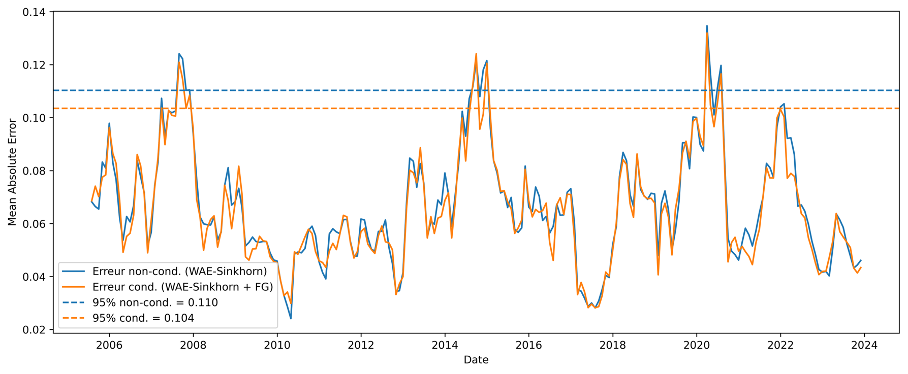
\includegraphics[width=0.9\linewidth]{images/results_ct.png}
    \caption{Erreurs de reconstruction superposées des modèles conditionnel et non conditionnel (court terme).}
    \label{fig:vae_lstm_short_term}
\end{figure}

\subsubsection{Effet de confirmation et de validation des signaux du marché}

Même si la FG n’apporte pas d’information supplémentaire significative dans la dynamique immédiate du stress systémique, elle joue un rôle important de signal de confirmation. La communication explicite de la banque centrale valide ou nuance les anticipations spontanées du marché, renforçant la crédibilité des prévisions économiques et financières.\\

Pour le régulateur, cela réduit l’incertitude liée à la prise de décision, en offrant une source d’information officielle et transparente, indispensable notamment dans des périodes de forte volatilité. Ainsi, même sans gains significatifs en termes de prédiction, la FG facilite la stabilité des anticipations, contribuant à limiter les mouvements excessifs des marchés. Ainsi, la FG peut atténuer les asymétries d’information entre les différents acteurs du marché et entre les agents économiques et le régulateur. À court terme, la disponibilité de signaux clairs issus de la politique monétaire permet une meilleure coordination des décisions, évitant que certains agents n’aient un avantage informationnel indu, facteur de volatilité et d’instabilité.\\

Cela peut avoir un impact indirect mais non négligeable sur le stress systémique, en limitant les comportements d’anticipation extrêmes ou les réactions disproportionnées à des rumeurs ou événements exogènes.

\subsubsection{Effet stabilisateur par la gestion des attentes}

La Forward Guidance contribue à orienter les anticipations des marchés financiers, même à court terme, en ancrant les attentes sur l’évolution future des conditions monétaires. Cette ancre comportementale réduit la probabilité d’ajustements brusques et inattendus, ce qui, en retour, diminue la probabilité d’une montée rapide du stress systémique. Pour le régulateur, c’est un outil précieux permettant de moduler les comportements de marché, notamment dans les phases de transition économique ou de crise naissante, en assurant une certaine fluidité dans les mécanismes de transmission de la politique monétaire.\\

Même si les marchés anticipent rapidement les chocs, la communication de la banque centrale par la FG peut influencer les conditions de liquidité à court terme, par exemple en rassurant les investisseurs sur la continuité du soutien monétaire. Cette influence indirecte sur les spreads de crédit, la volatilité ou les volumes échangés peut moduler le stress systémique, bien que cet effet ne soit pas directement observable dans la reconstruction statistique des signaux latents.

\subsubsection{Limites liées à la rapidité d’intégration des marchés}

La faible amélioration observée de la FG dans la reconstruction à court terme s’explique notamment par la sophistication et la rapidité d’adaptation des marchés financiers. Ceux-ci, en particulier les acteurs professionnels, intègrent très rapidement les informations publiques, rendant la FG redondante à ces horizons temporels.\\

Cela suggère que la valeur ajoutée de la FG réside davantage dans les horizons intermédiaires à longs termes, où la communication peut guider les anticipations et influencer durablement les comportements de marché, plutôt que dans la simple capacité à réduire les erreurs de prévision immédiates.

\subsubsection{Importance stratégique de la Forward Guidance dans la gestion des crises}

Enfin, même à court terme, la FG peut jouer un rôle stratégique en période de crise ou d’instabilité élevée. La communication claire et cohérente de la banque centrale peut prévenir des réactions de panique, en stabilisant les anticipations et en assurant aux marchés que des mesures de soutien sont en place ou envisagées. Cette fonction stabilisatrice, bien que difficile à quantifier dans les modèles à court terme, est essentielle pour le régulateur, qui doit non seulement comprendre le stress systémique, mais aussi agir pour le contenir.\\

À court terme, bien que la Forward Guidance ne semble pas améliorer significativement la capacité de reconstruction ou d’anticipation du stress systémique par rapport aux dynamiques endogènes du marché, ses effets pour le régulateur ne se limitent pas à la seule prédiction. Elle joue un rôle clé dans la réduction des incertitudes, la stabilisation des anticipations, la réduction des asymétries d’information, et la gestion des comportements de marché, particulièrement dans les phases critiques. Ces fonctions sont cruciales pour assurer la résilience du système financier, et justifient pleinement le recours à la Forward Guidance comme un outil complémentaire de la politique monétaire, même à court terme.\\

En définitive, si la Forward Guidance n’améliore que marginalement la qualité statistique des reconstructions du stress systémique à très court terme, elle joue néanmoins un rôle non négligeable dans la régulation qualitative des comportements de marché. En renforçant la lisibilité des intentions de la banque centrale, en réduisant les asymétries d’information et en stabilisant les anticipations, elle contribue à la résilience du système financier, même lorsqu’elle ne modifie pas directement les dynamiques observables du stress. Toutefois, ces effets demeurent limités par la rapidité d’intégration des marchés, ce qui tend à atténuer la portée immédiate des signaux de Forward Guidance. Il convient désormais de s’interroger sur l’effet différé de cette communication stratégique, en élargissant l’horizon temporel d’analyse. L’objectif est de déterminer si, au-delà de la réaction instantanée des marchés, la Forward Guidance parvient à façonner plus durablement les anticipations et à influencer la trajectoire latente du stress systémique. C’est ce qui est exploré dans la section suivante, consacrée à l’impact à moyen terme.

\subsection{Impact à moyen terme}

À l’horizon de 30 jours (considéré comme moyen terme), les effets différés de la communication de la BCE commencent à se manifester comme le montre la \autoref{fig:vae_lstm_mid_term}. Contrairement au court terme, où les modèles conditionnel et non conditionnel présentent des erreurs de reconstruction presque superposées, on observe ici une divergence plus marquée entre les deux dynamiques. En particulier, le modèle conditionnel  affiche une plus grande variabilité, avec des épisodes d’augmentation localisée de l’erreur — notamment durant les périodes de crise intense, comme la crise des dettes souveraines (2009–2015) et les turbulences associées à la pandémie de COVID-19 (2020–2021).

\begin{figure}[H]
    \centering
    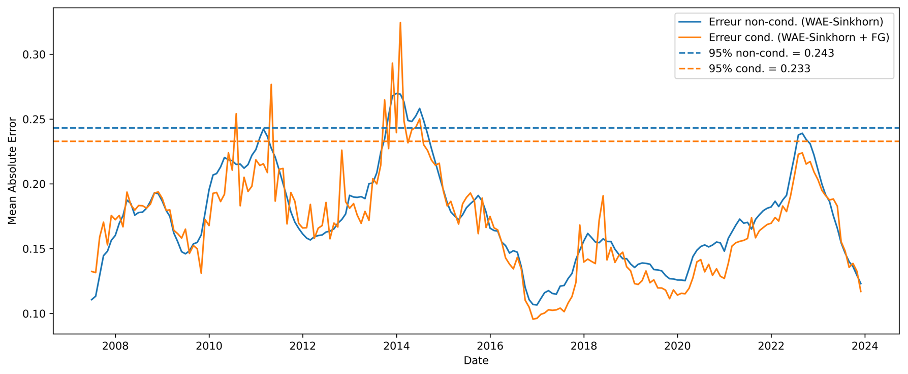
\includegraphics[width=0.9\linewidth]{images/results_mt.png}
    \caption{Erreurs de reconstruction superposées des modèles conditionnel et non conditionnel (moyen terme).}
    \label{fig:vae_lstm_mid_term}
\end{figure}

Bien que la moyenne des erreurs conditionnelles (MAE à 95\%) soit légèrement inférieure à celle du modèle non conditionné (0.233 vs 0.243), cette amélioration globale cache une instabilité structurelle : la courbe orange présente de fortes oscillations, surtout en contexte de stress économique, ce qui laisse entrevoir une difficulté du modèle à tirer parti de la FG lorsque le régime informationnel devient incertain.

\subsubsection{Un signal informatif, mais instable dans les phases de crise}

Ce comportement erratique du modèle conditionnel s’explique par plusieurs facteurs, d'une part, la variabilité accrue du discours en période de crise, durant les épisodes de forte incertitude macroéconomique, la FG devient souvent plus fréquente, plus nuancée et potentiellement plus ambiguë. D'autre part, la BCE ajuste son ton, introduit des précautions oratoires ou des formulations conditionnelles (« data-dependent », « à un rythme approprié », etc.), ce qui complique l’encodage sémantique fiable de la tonalité du discours. Le message devient moins clair et donc plus difficile à traduire dans l’espace latent vectoriel utilisé par les modèles conditionnels.\\

Ensuite, le décalage entre discours et action en situation de stress, la communication peut prendre une valeur stratégique pour temporiser les attentes, rassurer les marchés, gagner du temps. Cela peut produire une dissociation entre les intentions exprimées et les politiques effectivement mises en œuvre, créant un bruit informationnel qui altère la cohérence des projections basées sur la FG.\\

Cela est aussi dû à la réception biaisée ou instable des marchés. L’efficacité de la Forward Guidance repose sur sa crédibilité et sur la capacité des agents économiques à l’intégrer rationnellement dans leurs anticipations. Or, en période de crise, les comportements deviennent plus erratiques (effets de panique, mimétisme, changement de régime d’anticipation), réduisant la capacité de la FG à ancrer efficacement les attentes. Les marchés peuvent mal interpréter les signaux ou accorder davantage de poids aux indicateurs conjoncturels qu’aux intentions déclarées.\\

Enfn, la fragmentation sémantique dans les discours en période de crise est présente. Le discours de la BCE devient souvent moins unifié, avec une diversité de porte-parole (membres du Directoire, présidente, gouverneurs nationaux), chacun tenant un discours parfois légèrement divergent. Cette hétérogénéité de tonalité rend le signal agrégé plus difficile à interpréter pour les modèles d’apprentissage automatique.

\subsubsection{Un signal potentiellement contre-productif à moyen terme}

Dans ces conditions, la Forward Guidance peut devenir moins informative, voire contre-productive, à l’horizon de 30 jours. Les erreurs de reconstruction plus élevées dans certaines phases reflètent une situation paradoxale où l’ajout d’information exogène (ici la FG) ne réduit pas l’incertitude, mais au contraire accroît l’instabilité des prédictions du modèle.\\

Cela peut être interprété comme le retour d’un bruit communicationnel, où la complexité sémantique dépasse la capacité des encodeurs à extraire un signal directionnel robuste. Autrement dit, le modèle apprend une représentation « instable » du stress latent, trop influencée par des signaux discursifs ambigus ou contradictoires.

\subsubsection{Implications stratégiques pour les régulateurs}

Pour la BCE et les autres autorités monétaires, ces résultats soulèvent plusieurs enjeux stratégiques. Il ya clairement une nécessité de clarté accrue en période de crise : les régulateurs doivent veiller à délivrer une communication plus homogène, cohérente et lisible. Cela suppose de limiter les signaux contradictoires, d’harmoniser les discours entre les membres de l’institution, et d’éviter l’usage excessif de formulations conditionnelles qui ajoutent de la complexité sémantique.\\

En ce qui concerne l'encadrement du rôle de la FG dans les outils de gestion de crise, il ne faut pas surévaluer la capacité de la FG à stabiliser les anticipations à moyen terme durant une crise. Son efficacité diminue lorsque le bruit informationnel augmente. En ce sens, la FG doit être complémentaire à des actions crédibles, mesurables et rapides, et non un substitut à l’action monétaire.\\

Il est également possible de voir que la Forward Guidance n’est efficace que si elle s’inscrit dans une trajectoire crédible, soutenue par des décisions concrètes. Les écarts entre paroles et actes dégradent rapidement l’impact du discours, comme le montre l’augmentation de l’erreur conditionnelle dans les périodes où la politique monétaire est perçue comme hésitante ou tardive.\\

L'importance du contexte de réception pour la FG n’est pas perçue de manière uniforme dans tous les régimes économiques. Les régulateurs doivent intégrer cette réalité dans leur stratégie de communication : un même message peut être stabilisateur en période calme, mais source de confusion en période de stress. La Forward Guidance commence à produire un effet différé sur les dynamiques latentes du stress, mais cet effet est fortement dépendant du régime économique. En période de stabilité, la FG peut enrichir utilement l’information intégrée dans les modèles. En revanche, lors des crises, elle peut devenir difficile à encoder, instable, voire contre-productive. Cela plaide pour une utilisation contextualisée, prudente et stratégiquement coordonnée de cet instrument de communication, et pour un arbitrage intelligent entre clarté, cohérence et crédibilité.\\

Ces résultats à moyen terme révèlent une dynamique plus ambivalente de la Forward Guidance. Bien qu’un effet différé soit perceptible sur la trajectoire du stress systémique, sa stabilité et sa lisibilité s’amenuisent dès lors que le contexte devient incertain ou marqué par des tensions économiques aiguës. L’introduction du signal exogène issu des discours de la BCE, loin de toujours clarifier la trajectoire anticipée, peut en certaines circonstances introduire une volatilité supplémentaire dans la modélisation du stress. Cela souligne les limites de la Forward Guidance lorsqu’elle n’est pas adossée à une stratégie de communication cohérente et à une action monétaire perçue comme crédible. Dès lors, son efficacité ne dépend pas uniquement de sa fréquence ou de sa tonalité, mais surtout de la manière dont elle est perçue et interprétée par les marchés dans un environnement donné. Il reste à déterminer si, sur des horizons plus longs, la Forward Guidance parvient à dépasser ces limitations conjoncturelles. En d'autres termes, son impact s’inscrit-il dans une logique d’ancrage progressif des anticipations ou s’efface-t-il au fil du temps sous l’effet des chocs exogènes ? Il est dorénavant proposé d’examiner cette question en analysant les dynamiques observées à long terme.

\newpage

\subsection{Impact à long terme}

Les résultats empiriques obtenus à l’horizon de six mois dans la \autoref{fig:vae_lstm_long_term} mettent clairement en évidence la supériorité explicative du modèle conditionnel, c’est-à-dire celui intégrant l’indice directionnel de FG. L’écart entre les erreurs absolues moyennes (MAE à 95\%) est significatif : 0.166 pour le modèle conditionnel contre 0.213 pour le modèle non conditionné. Ce gain de performance reflète une capacité accrue à anticiper les évolutions latentes du stress systémique lorsque le modèle est informé par la tonalité des discours de la BCE.

\begin{figure}[H]
    \centering
    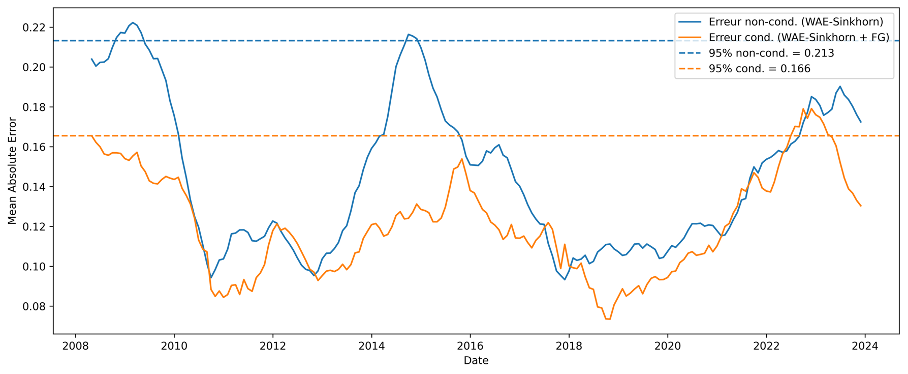
\includegraphics[width=0.9\linewidth]{images/results_lt.png}
    \caption{Erreurs de reconstruction superposées des modèles conditionnel et non conditionnel (long terme).}
    \label{fig:vae_lstm_long_term}
\end{figure}

Plus encore, l’analyse visuelle des trajectoires révèle des décalages temporels marqués entre les deux modèles, en particulier sur certaines périodes structurellement instables ou marquées par des transitions de régime monétaire — notamment entre 2011 et 2016 (phase post-crise souveraine en zone euro) et 2021 à 2023 (retour de l’inflation et réorientation vers une politique monétaire plus restrictive). Dans ces moments charnières, le modèle conditionnel parvient non seulement à anticiper l’intensification du stress, mais aussi à capter ses fluctuations différées, en lien avec les ajustements graduels des anticipations de marché.

\subsubsection{Un signal sémantique à effet différé : transmission longue de la FG}

L’analyse de ces résultats suggère une propriété centrale de la Forward Guidance : son impact sur le stress systémique est temporellement différé. Contrairement aux interventions monétaires directes (taux, opérations de refinancement, achats d’actifs), qui peuvent produire des effets immédiats sur la liquidité ou les prix d’actifs, la FG opère principalement via les anticipations. Les canaux par lesquels la FG influence le stress latent sont fondamentalement intertemporels.\\

D'abord, le canal des anticipations de taux futurs avec les déclarations orientent les croyances des agents économiques sur la trajectoire future des taux directeurs. Ces ajustements progressifs des anticipations affectent les décisions d’investissement, de crédit et de couverture avec un temps de latence significatif. Ensuite, le canal de crédibilité institutionnelle : une communication cohérente et récurrente renforce la confiance des marchés dans la capacité de la BCE à agir en cohérence avec ses annonces. Cette confiance ne se construit pas instantanément, mais s’accumule sur plusieurs mois, expliquant pourquoi l’indicateur directionnel devient plus prédictif à long terme. Enfin, le canal d’ancrage des anticipations d’inflation et de risque systémique où la FG contribue à stabiliser les anticipations macroéconomiques de long terme (inflation, croissance, volatilité financière), ce qui modère ex post la survenance de chocs de stress à horizon éloigné.\\

Ainsi, la baisse marquée de l’erreur du modèle conditionnel à 6 mois s’explique par le fait que la FG agit comme un indicateur avancé des futurs déséquilibres systémiques, mais que son impact ne se matérialise que dans un second temps — après diffusion dans les comportements d’allocation de portefeuille, les ajustements de bilans bancaires ou encore la reconfiguration des régimes de risque.

\subsubsection{Rôle différencié de la FG selon le régime macro-financier}

Les résultats montrent également que la valeur informative de la FG varie selon le contexte et le régime. En période de stabilité (par exemple 2013–2016), la FG joue un rôle de signal anticipatif puissant, guidant les marchés de manière douce et prévisible. Les discours de la BCE ont alors un effet de stabilisation stratégique, permettant aux acteurs de se repositionner graduellement, ce qui se traduit par une réduction effective du stress latent.\\

En période de transition ou de tension sous-jacente (par exemple 2021–2023), la FG agit comme un révélateur de rupture. La sémantique change, les mots employés deviennent plus restrictifs, ce qui précède — parfois de plusieurs mois — les inflexions effectives de la politique monétaire. Ces inflexions sont captées par les marchés dans un second temps, ce qui explique pourquoi le modèle conditionnel permet de détecter des ruptures anticipées dans les dynamiques du stress.\\

En période de crise ouverte, la FG ne semble pas être la source principale de variation du stress comme montré précédemment à moyen terme. Toutefois, à long terme, une communication résolument accommodante ou un changement de cap affirmé peut finir par rassurer les marchés, induisant une décrue progressive du stress systémique (exemple : les annonces de Draghi en 2012 « whatever it takes »).

\subsubsection{Implications de politique économique}

Ces résultats ont plusieurs implications fondamentales pour les régulateurs, en particulier les banques centrales et les autorités macroprudentielles. La Forward Guidance est un instrument stratégique de moyen-long terme : elle ne doit pas être évaluée uniquement à l’aune de ses effets instantanés. Son efficacité se manifeste dans sa capacité à préparer les ajustements structurels, à façonner les anticipations, et à ancrer la trajectoire future des politiques économiques.\\

La stabilité, la clarté et la cohérence de la communication sont cruciales, plus la communication est lisible, plus l’effet différé est net. Cela appelle une gestion rigoureuse de la séquence des discours, un encadrement strict des divergences narratives internes à l’institution, et un suivi continu des effets sémantiques.\\

La FG peut être utilisée comme indicateur avancé de stress latent dans une logique de prévention : au-delà de sa fonction de transmission, la tonalité agrégée des discours constitue un signal exploitable pour calibrer les politiques macroprudentielles, anticiper les points de rupture potentiels ou déclencher des mesures de soutien préventives. Aussi, l’efficacité différée de la FG invite à combiner les horizons de pilotage : une politique monétaire efficace doit s’articuler sur plusieurs niveaux temporels : instruments à effet immédiat (taux, opérations de marché), mécanismes de stabilisation de moyen terme (filet de sécurité bancaire, interventions ciblées), et communication de long terme visant les anticipations.\\

L’analyse empirique montre que, parmi les différents horizons temporels étudiés, c’est à long terme que la Forward Guidance révèle toute sa puissance explicative. Sa nature discursivement anticipative, son ancrage institutionnel et sa capacité à structurer les anticipations macro-financières en font un instrument d’orientation des comportements économiques plus qu’un outil de réaction immédiate. Les performances du modèle conditionnel indiquent que la tonalité des discours de la BCE est fortement corrélée, avec un décalage temporel, aux évolutions latentes du stress systémique. Cela confirme empiriquement la dimension stratégique de la communication monétaire, non seulement comme outil d’accompagnement, mais aussi comme mécanisme d’amortissement et de pilotage à horizon long dans la gestion des risques systémiques.\\

Ainsi, l’analyse à long terme met clairement en lumière la dimension stratégique de la Forward Guidance dans le pilotage du stress systémique. Contrairement aux horizons plus courts, où ses effets peuvent être atténués par la rapidité d’ajustement des marchés, son rôle se révèle pleinement lorsqu’on observe les dynamiques financières sur des périodes étendues. La communication monétaire, lorsqu’elle est cohérente, lisible et inscrite dans un cadre institutionnel stable, constitue un levier puissant pour orienter les anticipations collectives, amortir les transitions de régime et stabiliser progressivement les équilibres systémiques. Le caractère différé de son efficacité impose toutefois une vigilance accrue quant à la qualité du signal émis, à la clarté du message délivré et à la synchronisation entre les intentions exprimées et les instruments mobilisés. L’analyse appelle désormais une réflexion plus normative : comment les régulateurs, et en particulier la Banque centrale européenne, peuvent-ils optimiser l’usage de la Forward Guidance dans leur arsenal d’intervention ? Quelles recommandations concrètes peut-on formuler en matière de communication, de coordination inter-institutionnelle ou de conception des outils macroprudentiels ? La section suivante propose de répondre à ces interrogations en formulant un ensemble de recommandations opérationnelles à destination des autorités monétaires et de supervision.

\subsection{Recommandations opérationnelles pour la BCE et les autorités macroprudentielles}

Les résultats empiriques présentés dans ce chapitre ont mis en évidence le rôle différencié de la Forward Guidance (FG) selon les horizons temporels et les régimes macro-financiers. Si son effet est limité à court terme, la FG se révèle particulièrement efficace à moyen et long termes, notamment en tant qu’ancre anticipative des comportements de marché. Afin de renforcer cette efficacité, plusieurs recommandations opérationnelles peuvent être formulées à destination de la Banque Centrale Européenne (BCE) et, plus largement, des autorités chargées de la stabilité financière. Ces recommandations visent à améliorer la clarté, la crédibilité et la cohérence de la communication monétaire, en articulant plus étroitement les messages sémantiques et les instruments de politique économique.

\subsubsection{Renforcer la cohérence et la traçabilité de la communication monétaire}

Il a été observé que la fragmentation de la communication institutionnelle, notamment dans les phases de crise, tend à générer du bruit sémantique, compromettant la lisibilité des signaux monétaires. Cette hétérogénéité, souvent causée par la multiplicité des porte-parole ou par des divergences narratives entre les membres du Conseil des gouverneurs, se traduit par une volatilité accrue du stress latent. Afin de limiter ce phénomène, une harmonisation de la voix institutionnelle doit être systématiquement recherchée. Cela peut passer par l’instauration d’un calendrier officiel structurant les prises de parole prioritaires (notamment celles de la présidence ou du chef économiste) et par la définition ex ante de lignes directrices sémantiques à respecter dans les communications publiques.

Par ailleurs, la crédibilité de la FG pourrait être consolidée en l’adossant à des jalons d’action observables. Il serait opportun que les annonces de politique monétaire fassent explicitement référence à des seuils ou des indicateurs vérifiables, tels que le taux d’inflation sous-jacent, la dispersion des primes de risque souverain ou le niveau d’output gap. L’adoption d’une matrice condition–action, même simplifiée, renforcerait la transparence du processus de décision, tout en préservant une marge d’ajustement. Une communication exprimée sous forme de plages cibles, plutôt que de points fixes, permettrait d’éviter toute rigidité excessive, tout en maintenant une orientation stratégique.

\subsubsection{Mettre en place un système de suivi sémantique intégré et réactif}

L’efficacité de la communication de politique monétaire repose en grande partie sur la clarté, la cohérence et la stabilité des signaux transmis. Dans cette perspective, il apparaît essentiel de doter l’autorité monétaire d’un système de suivi sémantique capable de capter en temps réel les inflexions discursives et d’en mesurer l’impact potentiel sur les anticipations de marché. Une telle infrastructure permettrait d’objectiver le contenu sémantique des discours, d’assurer leur alignement avec les objectifs stratégiques de la politique monétaire, et de prévenir les dissonances narratives susceptibles d’accroître l’incertitude ou de générer un stress financier inutile.\\

À cet effet, il est proposé la mise en place d’un tableau de bord dédié à l’analyse de la Forward Guidance, dont la conception pourrait s’inspirer des méthodes développées dans la présente étude. Ce tableau de bord intégrerait plusieurs indicateurs complémentaires, actualisés à chaque nouvelle publication institutionnelle. Tout d’abord, une mesure directionnelle, analogue à l’indice $z_t$, permettrait de quantifier la tonalité sémantique de chaque discours selon un axe latent allant de l’accommodant au restrictif. Cette mesure serait calculée sur la base d’un encodage sémantique automatisé, projeté sur une direction vectorielle construite à partir de phrases d’ancrage générées et validées selon une procédure standardisée. En complément, un indicateur de dispersion inter-locuteur pourrait être introduit afin de mesurer l’hétérogénéité des positions discursives entre les différents membres du Conseil des gouverneurs. Ce coefficient de dispersion, calculé par exemple comme l’écart-type des scores $z_t$ sur une période donnée, permettrait d’identifier les périodes où les signaux envoyés aux marchés apparaissent ambigus ou contradictoires. Une telle situation est généralement corrélée à une perte de lisibilité de la stratégie monétaire, et peut induire une volatilité excessive, comme le suggèrent les résultats empiriques observés à moyen terme dans les phases de crise.\\

Par ailleurs, une métrique de stabilité temporelle devrait être ajoutée, par exemple sous la forme d’une variance mobile des scores sémantiques sur un horizon glissant de plusieurs semaines ou mois. Cette mesure permettrait de suivre la cohérence inter-temporelle de la communication, et de détecter d’éventuels glissements discursifs non intentionnels. Une montée soudaine de la variance sémantique constituerait ainsi un signal d’alerte, susceptible de déclencher une intervention corrective.\\

Afin de donner une portée opérationnelle à ce tableau de bord, il conviendrait d’y associer un mécanisme de gouvernance. Il est proposé que des seuils d’alerte soient fixés pour chacun des indicateurs, de manière à identifier les situations nécessitant une réponse institutionnelle. En cas de dépassement de ces seuils, un comité éditorial interne pourrait être mobilisé. Sa mission consisterait à analyser les causes de la divergence sémantique, à recommander des ajustements de formulation, voire à coordonner les prochaines prises de parole afin de rétablir l’unité narrative. Ce comité, composé de représentants de la direction de la communication, du département de politique monétaire et du secrétariat général, jouerait un rôle central dans la régulation qualitative de la FG.\\

Parallèlement, il apparaît souhaitable d’exploiter les avancées récentes en NLP pour automatiser une partie de ce suivi. L’usage de modèles de type transformeurs, notamment BERT, Mamba ou Llamba, permettrait de mettre en œuvre des outils de surveillance sémantique en temps réel. Grâce à des techniques d’attention contextuelle et de classification latente, il deviendrait possible de détecter automatiquement les glissements de tonalité, les ruptures stylistiques, ou encore les contradictions implicites entre différents segments de discours. Cette surveillance algorithmique, couplée à une interface visuelle interactive, constituerait un appui précieux pour les responsables de la communication stratégique. Toutefois, le pilotage qualitatif de la FG ne saurait se limiter à un contrôle ex ante. Une démarche d’évaluation ex post s’impose, à l’image de ce qui est pratiqué pour les outils non conventionnels tels que les programmes d’achats d’actifs. Il serait donc recommandé de publier, à intervalles réguliers (par exemple semestriellement), un rapport d’évaluation de la communication monétaire. Ce rapport relierait, à l’aide de méthodes économétriques rigoureuses, les caractéristiques sémantiques des discours publiés à l’évolution des indicateurs de stress systémique, des spreads de taux d’intérêt, ou encore de la volatilité implicite sur les marchés financiers.\\

En cas d’écart significatif entre les effets attendus de la FG et les dynamiques observées sur les marchés, une révision des stratégies discursives pourrait être envisagée. Cette révision porterait soit sur le contenu (simplification du message, clarification des intentions), soit sur la forme (choix du canal de communication, fréquence des publications, identité du parleur). Ainsi, le lien entre analyse sémantique et pilotage stratégique serait pleinement institutionnalisé.

\subsubsection{Intégrer la Forward Guidance dans une architecture de réponse coordonnée aux chocs}

Les résultats empiriques ont révélé que, durant les périodes de forte instabilité, la FG ne produit ses effets que lorsqu’elle est accompagnée de mesures tangibles. La communication verbale, lorsqu’elle est isolée, tend à perdre de sa capacité d’ancrage. Dès lors, une coordination renforcée entre FG et instruments de liquidité s’impose. Les annonces de FG gagneraient à être systématiquement couplées à la publication de calendriers d’intervention, à l’annonce des montants prévus ou à la réactivation de dispositifs ciblés tels que les T-LTRO, PELTRO ou lignes de swap. Cette approche conjointe permettrait d’amplifier l’effet de signal et de renforcer la crédibilité de la trajectoire annoncée. Par ailleurs, la FG devrait être articulée de manière plus explicite avec la politique macroprudentielle. Les outils tels que le coussin contracyclique, les réserves obligatoires différenciées ou les orientations sectorielles devraient être calibrés en cohérence avec les signaux sémantiques envoyés par la BCE. Une telle coordination réduirait le risque de messages contradictoires et renforcerait l’efficacité globale du cadre de stabilisation financière. Enfin, les résultats suggèrent qu’une adaptation de la granularité temporelle de la FG est nécessaire. Étant donné l’efficacité différée de la communication observée à l’horizon de six mois, il conviendrait de privilégier une guidance explicite pour les thématiques de moyen et long termes (politique de bilan, trajectoire des taux d’intérêt nominaux), tout en maintenant une guidance plus qualitative ou contingente à court terme. Cette flexibilité temporelle permettrait d’éviter les effets de sur-interprétation immédiate, tout en assurant un encadrement stratégique durable des anticipations. L’ensemble de ces recommandations vise à faire de la Forward Guidance non plus seulement un vecteur d’intentions, mais un instrument intégré à l’architecture de stabilisation macro-financière. Lorsqu’elle est bien faite, la communication de la BCE peut devenir un puissant levier de réduction du stress systémique, en particulier sur les horizons temporels où les canaux de transmission sont les plus actifs.

\newpage

Ce chapitre a proposé une architecture intégrée pour analyser empiriquement l’impact de la Forward Guidance sur le stress systémique, à l’aide de méthodes avancées en traitement automatique du langage naturel et en modélisation de séries temporelles. L’objectif principal était d’établir une passerelle rigoureuse entre les signaux sémantiques émis par la Banque centrale européenne et les dynamiques latentes de vulnérabilité financière, en montrant que le langage de politique monétaire, loin d’être un simple artefact rhétorique, constitue une variable économique de premier plan.\\

La première étape de cette analyse a consisté à encoder la tonalité des discours de politique monétaire. Pour cela, un indicateur directionnel de Forward Guidance a été construit en projetant chaque document textuel dans un espace sémantique latent, à l’aide de modèles de langage pré-entraînés. Des architectures distinctes, telles que ModernBERT, Mamba, Mamba-2 et Llamba, ont été mobilisées pour produire des représentations vectorielles de haute dimension, à partir desquelles des scores directionnels ont été extraits par projection dans un axe discursif structuré allant du registre restrictif vers l’orientation expansionniste. L’évaluation comparative de ces représentations, via des régressions Ridge appliquées à un indicateur de stress financier comme le CISS, a permis de sélectionner les encodeurs offrant la meilleure capacité explicative du stress systémique pour Mamba. Sur cette base, un modèle d’autoencodeur Wasserstein-LSTM conditionnel a été développé afin de capturer les dynamiques structurelles du stress latent. Ce modèle s’appuie sur la régularisation de l’espace latent via une contrainte de transport optimal, assurant une géométrie probabiliste cohérente, tout en permettant d’intégrer de manière conditionnelle les signaux exogènes issus de la Forward Guidance. Cette architecture a été appliquée aux séries temporelles financières découpées en fenêtres glissantes, afin d’en reconstruire l’évolution à différents horizons temporels, en comparant les erreurs issues d’un modèle conditionné par la FG à celles d’un modèle non informé.\\

Les résultats empiriques ont révélé une hétérogénéité significative des effets de la Forward Guidance selon l’horizon temporel. À très court terme, la valeur ajoutée de la communication apparaît limitée : les marchés financiers, par leur nature hautement réactive, semblent intégrer rapidement les signaux disponibles, rendant la FG redondante d’un point de vue prédictif. Toutefois, cette observation ne doit pas masquer le rôle stratégique que joue la FG dans la réduction des incertitudes, la stabilisation des anticipations, et la prévention des asymétries informationnelles. La FG agit comme une boussole narrative, utile pour encadrer les interprétations de marché même lorsqu’elle ne modifie pas substantiellement les trajectoires. À moyen terme, les effets deviennent ambigus. En période de stabilité relative, la FG peut continuer à guider les anticipations de manière efficace. En revanche, en période de crise ou d’incertitude accrue, la complexité sémantique des discours, (due à l’usage accru de formulations conditionnelles, à la multiplicité des porte-parole, ou à des ajustements tactiques dans la communication) peut altérer la lisibilité du signal. Cette dégradation du contenu informationnel se traduit, dans les modèles conditionnels, par une instabilité accrue des reconstructions, voire par une perte de performance prédictive. Ce paradoxe – où un excès de communication nuit à la capacité d’anticipation souligne les limites opérationnelles de la Forward Guidance en contexte de stress aigu. C’est à long terme que la puissance explicative de la Forward Guidance s’affirme avec le plus de netteté. Les modèles conditionnels surpassent de manière robuste les versions non conditionnelles, tant en termes d’erreur moyenne que de capacité à détecter les transitions de régime. Cette supériorité s’interprète comme la manifestation différée d’un canal d’anticipation structurel : en orientant les croyances sur les trajectoires futures de la politique monétaire, la FG influence les décisions d’investissement, la gestion des risques, et les arbitrages de portefeuille, avec un effet amorti mais cumulatif. L’ancrage des anticipations opère donc dans un espace-temps élargi, compatible avec la temporalité des ajustements macro-financiers.\\

L’utilisation d’architectures issues du deep learning se justifie donc par la nature même des données mobilisées et des dynamiques recherchées. Les méthodes traditionnelles, fondées sur des hypothèses linéaires ou paramétriques fortes, se heurtent à la complexité structurelle des séries financières et à la richesse sémantique des discours de politique monétaire. En effet, le langage de la Forward Guidance ne suit pas une syntaxe standardisable ni des relations fixes entre variables, mais mobilise des tournures implicites, conditionnelles ou stratégiques, difficilement capturables par des modèles linéaires classiques. De même, les trajectoires du stress systémique obéissent à des régimes multiples, parfois latents, dont les transitions ne peuvent être appréhendées de manière satisfaisante par des approches stationnaires. En combinant des modèles de langage non supervisés, capables de structurer l’information textuelle dans des espaces latents complexes, avec des autoencodeurs dynamiques régularisés par le transport optimal, le deep learning offre une capacité unique à extraire, intégrer et projeter des signaux discontinus et multidimensionnels. Ce paradigme permet non seulement une meilleure reconstruction des dynamiques observées, mais aussi une modélisation plus réaliste des mécanismes d’anticipation et de propagation du stress. Il ne s’agit donc pas d’un simple choix technique, mais d’un cadre méthodologique cohérent avec l’hypothèse d’une économie informationnellement dense, où la communication devient une variable structurelle à part entière.\\

Ces résultats soulignent le caractère intertemporel de la FG, qui se distingue fondamentalement des instruments traditionnels de politique monétaire. Là où les taux d’intérêt ou les programmes d’achat produisent des effets immédiats, la FG agit par diffusion lente à travers les canaux de communication, de crédibilité et de coordination. Elle constitue un levier de stabilisation dont l’efficacité repose sur la cohérence narrative, la lisibilité des signaux, et l’alignement entre intentions déclarées et actions réelles. En définitive, ce chapitre apporte une double contribution : méthodologique, en proposant une chaîne de traitement unifiée combinant NLP avancé et modélisation du stress latent ; et empirique, en mettant en évidence la nature temporellement différée et stratégiquement conditionnée de l’impact de la Forward Guidance sur le stress systémique. Il en résulte une perspective renouvelée sur le rôle de la communication monétaire, non pas comme simple accompagnement rhétorique des décisions, mais comme instrument actif de gestion des risques financiers. Cette perspective invite à repenser la place de la FG dans les outils de régulation contemporains, et appelle à une réflexion approfondie sur les conditions de son efficacité. C’est à cette réflexion opérationnelle que s'est consacré cette étude.
\chapter*{Conclusion}
\addcontentsline{toc}{chapter}{Conclusion}

Dans ce mémoire il a été démontré l’impact de la Forward Guidance de la Banque Centrale Européenne sur le stress systémique au sein de la zone euro mesuré par le CISS, en mobilisant des outils de NLP et d’apprentissage profond. Ainsi, dans ce mémoire, sur la base d’une approche textuelle, computationnelle et empirique, il a été montré dans quelle mesure la communication anticipative de la BCE permettait de réduire les tensions sur les marchés financiers, ou au contraire, pouvait les amplifier en période d’incertitude sur une période hebdomadaire allant de janvier 2005 à décembre 2024 sur données hebdomadaires.\\

Une analyse historique et conceptuelle a d'abord permis de retracer l’évolution du rôle de la forward guidance dans l’arsenal de la politique monétaire européenne. Apparue initialement comme une réponse à la borne inférieure des taux d’intérêt nominaux, la FG s’est progressivement institutionnalisée comme un instrument stratégique, mobilisé tant dans des contextes expansionnistes que restrictifs. Cependant, cette montée en puissance s’est accompagnée de nombreuses interrogations sur ses canaux de transmission, sa crédibilité, et son efficacité face aux chocs macro-financiers. Aussi, le concept de stress systémique s’est imposé comme une dimension centrale de la stabilité financière, incarnée notamment par la création de l’indicateur composite de stress systémique par la BCE. Contrairement aux simples mesures de volatilité, le stress systémique capte les dynamiques de contagion, les ruptures de confiance et les interdépendances entre marchés. Il constitue dès lors un outil pertinent pour étudier les effets potentiels de la communication monétaire sur l’architecture financière dans son ensemble.\\

Le mémoire a introduit une méthodologie innovante, articulée autour de l’analyse sémantique des discours de la Banque Centrale Européenne. Cette étape a consisté à mobiliser des modèles de langage de nouvelle génération, parmi lesquels ModernBERT, Mamba, Mamba-2 et Llamba, capables de capturer des représentations contextuelles fines et hiérarchisées des textes. Ces modèles, fondés sur des architectures de type transformeur ou espace d’état, ont permis d’extraire des vecteurs sémantiques à haute dimension, à partir desquels un indicateur directionnel de tonalité a été construit. Ce score continu, projeté dans un espace latent structuré, permet de quantifier la posture implicite de la BCE à chaque instant, sur un axe allant de l’orientation expansionniste à la posture plus restrictive. L’indicateur a été calculé pour l’ensemble des discours officiels de la BCE sur une période couvrant près de vingt ans (janvier 2005 à décembre 2024), intégrant ainsi une large diversité de contextes macroéconomiques et de régimes monétaires. Cette modélisation sémantique permet non seulement de saisir les nuances lexicales des communiqués, mais également de rendre compte des transitions progressives dans les discours, des inflexions de ton et des variations de cadre rhétorique (selon le président). Dans une dernière phase, cet indicateur a été intégré dans des modèles dynamiques de séries temporelles, afin d’en évaluer l’effet sur la trajectoire latente du stress systémique. À cette fin, des réseaux récurrents de type LSTM ont été mobilisés pour modéliser la dépendance séquentielle des données financières, tandis que l’espace latent a été régularisé par des techniques issues des Wasserstein Auto-Encoders. Cette approche a permis d’imposer une géométrie probabiliste cohérente à la représentation du stress, tout en autorisant une injection conditionnelle des signaux de forward guidance. L’ensemble du dispositif a ainsi permis d’évaluer, de manière intégrée, la capacité de la communication monétaire à influencer les dynamiques de vulnérabilité financière.\\

Les résultats empiriques mettent en évidence une hétérogénéité marquée dans l’impact de la FG selon l’horizon temporel et les régimes macro-financiers. À court terme, les résultats empiriques montrent que l’intégration de la FG dans les modèles conditionnels n’entraîne qu’une amélioration marginale des erreurs de reconstruction du stress systémique. Cette faible valeur ajoutée s’explique par la forte réactivité des marchés financiers, qui absorbent rapidement les informations publiques et ajustent leurs anticipations en conséquence. Néanmoins, la FG demeure un levier pertinent pour la stabilisation dans l'ancrage des agents économiques. Elle contribue à réduire l’asymétrie  entre acteurs, en clarifiant les intentions de la banque centrale, et permet d’aligner plus efficacement les décisions des participants de marché sur un cadre commun. Son utilité réside donc des les anticipations collectives, en particulier en période de transition ou d’incertitude modérée. À l’horizon moyen terme (environ 30 jours), les effets de la FG deviennent plus ambigus. En contexte de stabilité macro-financière, la tonalité des discours conserve une valeur explicative modérée : elle continue d’influencer la dynamique latente du stress en guidant progressivement les réajustements de portefeuille et les anticipations de liquidité. Toutefois, dans les épisodes de crise ou d’incertitude aiguë, la cohérence des signaux émis par la BCE s’affaiblit. Le recours accru à des formulations conditionnelles, la multiplication des voix institutionnelles, et les différences de tons complexifient le traitement automatique du signal. Les performances du modèle conditionnel deviennent alors plus volatiles, et peuvent se dégrader par rapport au modèle non conditionné, traduisant un bruit accru. La FG peut, dans ces conditions, introduire une incertitude supplémentaire, en altérant la lisibilité globale des marchés. À long terme, les résultats suggèrent que l’introduction de la Forward Guidance dans le modèle conditionnel n'améliore pas la capacité à anticiper les dynamiques latentes du stress systémique. Bien que les erreurs moyennes soient plus faibles en moyenne pour le modèle conditionnel, une observation plus fine des trajectoires révèle un retard persistant dans la dynamique reconstruite. La courbe du modèle conditionnel apparaît régulièrement décalée vers l’aval, indiquant que l’information contenue dans les discours de la BCE est intégrée avec un temps de latence (environ 6 mois), et que la Forward Guidance agit davantage comme un révélateur a posteriori que comme un signal prédictif immédiat. Ce décalage temporel peut s’interpréter comme le reflet d’un processus lent de transmission des signaux discursifs vers les anticipations effectives des agents économiques. Contrairement aux instruments directs de politique monétaire, la Forward Guidance ne produit pas d’effet instantané : sa réception, son interprétation et son incorporation dans les arbitrages financiers nécessitent un temps d’ajustement. Les comportements d’investissement, de couverture ou de refinancement peuvent ne répondre que progressivement aux inflexions de langage, surtout lorsque le discours reste ambigu, conditionnel ou sujet à interprétation. Ainsi, la tonalité agrégée des discours ne constitue pas ici un indicateur avancé du stress, mais plutôt un signal coïncident voire légèrement retardé dans les phases de tensions systémiques. Cela ne remet pas en cause la pertinence de la FG comme outil stratégique, mais souligne la nécessité de mieux encadrer ses modalités de diffusion et de renforcer sa lisibilité. Un discours plus clair, mieux synchronisé avec les autres instruments de politique économique, pourrait réduire ce décalage et renforcer l’efficacité temporelle de la communication anticipative.

\newpage

Il apparaît que la FG ne peut être traitée comme un instrument isolé : son efficacité dépend de la complémentarité avec d’autres leviers de politique monétaire et macroprudentielle. En période d’incertitude accrue, la simple émission de signaux verbaux, non assortis de mesures concrètes, tend à perdre de son impact. La coordination inter-institutionnelle (banques centrales, régulateurs prudentiels, autorités budgétaires) devient alors essentielle pour renforcer la crédibilité du signal. Ensuite, la stabilité des anticipations dépend fortement de la clarté sémantique et de la constance temporelle des messages. Une forward guidance changeante, ambiguë ou après coup modifiée peut engendrer de l’instabilité interprétative, en particulier dans des contextes de fragmentation des marchés ou de divergence des anticipations nationales. D’où l’importance d’un ancrage linguistique cohérent. En outre, les résultats empiriques de ce mémoire confirment que les outils issus de l’intelligence artificielle (IA) peuvent jouer un rôle croissant dans l’analyse de la politique monétaire. En capturant des dimensions sémantiques fines, ces modèles permettent de construire des indicateurs dynamiques sensibles aux évolutions discursives, et utiles à la fois pour l’analyse académique et pour le suivi opérationnel par les autorités.\\

Dans cette perspective, plusieurs enseignements opérationnels peuvent être formulés à destination des régulateurs. D’abord, les résultats plaident en faveur d’une structuration plus rigoureuse de la communication monétaire. Lorsque les messages sont multiples, fragmentés ou conditionnels, leur valeur informative s’amenuise. Il serait pertinent que les autorités adoptent des lignes directrices plus explicites en matière de tonalité et de constance des discours, en particulier en période de crise, où les risques d’interprétation divergente sont amplifiés. Cela implique de mieux coordonner les prises de parole entre les membres des comités de politique monétaire et de limiter les écarts narratifs susceptibles de brouiller la lecture des signaux par les agents économiques. Ensuite, il apparaît nécessaire de renforcer le lien  de la Forward Guidance à des actions mesurables. Les annonces doivent être accompagnées de points observables, comme des plages de taux, des seuils macroéconomiques ou des éléments calendaires, afin de maximiser leur pouvoir d’ancrage. La parole seule ne suffit que si elle s’inscrit dans un continuum stratégique crédible. À cet égard, la guidance devrait être systématiquement articulée avec les outils de liquidité pour éviter tout écart entre les intentions déclarées et les instruments effectivement mobilisés.\\

Il serait également recommandé d’intégrer la FG dans un système de suivi sémantique en temps réel. Les banques centrales pourraient tirer parti des techniques de traitement du langage développées ici pour surveiller l’évolution de la perception externe de leur communication. Des tableaux de bord internes, fondés sur des modèles de langage modernes, pourraient permettre d’évaluer en continu la stabilité, la dispersion et la direction des signaux envoyés. En cas de divergence marquée ou d’instabilité dans la tonalité perçue, des ajustements correctifs pourraient être envisagés rapidement. Ce qui permettrait de renforcer l’agilité de la politique monétaire dans un environnement actuel pris dans les crises. Enfin, la temporalité différée de l’effet de la Forward Guidance appelle à une révision des horizons de pilotage des régulateurs. Il ne suffit pas de mesurer l’impact immédiat d’une communication sur les marchés pour en juger la pertinence. Il convient de suivre son influence sur les anticipations et la structure des bilans bancaires à moyen et long termes. Cette approche multi-horizons permettrait d’éviter une focalisation excessive sur les réactions de court terme, souvent bruitées, au profit d’une évaluation plus différée.\\

Cependant, plusieurs limites demeurent et ouvrent la voie à de nouvelles pistes de recherche. L’analyse a été centrée sur les discours institutionnels de la BCE. Il serait intéressant d’y intégrer les discours décentralisés ou encore les échos médiatiques, pour cartographier la diffusion effective des signaux de forward guidance. De plus, les modèles de langage utilisés reposent sur des bases généralistes : l'entraînement sur des corpus spécifiquement monétaires pourrait améliorer leur sensibilité aux nuances techniques et macroéconomiques. Enfin, une ouverture majeure réside dans l’analyse de l’espace latent généré par les Wasserstein Auto-Encoders. Si ceux-ci permettent d’inférer des représentations structurellement régularisées du stress systémique, l’espace latent résultant pourrait faire l’objet d’une exploration plus approfondie. Il serait notamment prometteur de développer des méthodes capables de détecter les points de retournement structurels dans cet espace c’est-à-dire des configurations latentes préfigurant un changement de régime, une contagion accrue ou un basculement de la dynamique systémique. À terme, une formalisation géométrique plus riche de cet espace latent pourrait être envisagée. En s'appuyant sur des hypothèses de courbure issues de la géométrie riemannienne, par exemple via l’utilisation de variétés à courbure négative, il serait alors possible de structurer l’espace latent de manière à mieux refléter les transitions non linéaires. Cette perspective ouvre un champ de recherche à la croisée de la géométrie différentielle, du deep learning et de l’analyse de la politique monétaire. Dans un monde financier interconnecté, comprendre la morphologie des signaux latents et leur évolution pourrait fournir un avantage décisif pour anticiper les vulnérabilités systémiques. En somme, l’intelligence artificielle ne constitue pas seulement un outil d’analyse, mais bien un nouvel outil pour la stabilité systémique.\\

Enfin, une ouverture complémentaire peut être formulée autour de l’étude des mécanismes de contagion financière et macroéconomique, en particulier au sein du système interbancaire européen. Si le stress systémique a été ici modélisé sous la forme d’une trajectoire latente globale, reflétant les tensions agrégées sur les principaux marchés financiers, il demeure possible d’affiner cette lecture en analysant la manière dont ce stress se diffuse au sein du réseau bancaire. Le système interbancaire constitue en effet un vecteur privilégié de transmission des chocs de liquidité, des ruptures de confiance et des ajustements de portefeuilles induits par les signaux de politique monétaire. L’architecture WAE-LSTM développée dans ce mémoire pourrait ainsi être adaptée pour intégrer explicitement des données de réseau bancaire, telles que les expositions croisées. Une telle extension permettrait d’identifier si, et comment, les signaux de Forward Guidance contribuent à amplifier ou atténuer les dynamiques de contagion entre banques. Par exemple, une communication perçue comme restrictive pourrait accroître les tensions de liquidité en périphérie du réseau, provoquant une fragmentation accrue du marché interbancaire. Inversement, une guidance perçue comme crédible et coordonnée pourrait renforcer la confiance mutuelle et réduire les besoins de précaution au bilan, limitant ainsi la propagation du stress. L’analyse des effets de la FG dans l’architecture financière pourrait ainsi devenir un axe à part entière. Plus largement, cette perspective invite à repenser la politique monétaire comme un processus d’influence systémique multi-échelle. Au-delà de son impact agrégé sur les anticipations de marché, la Forward Guidance produit des effets différenciés selon la position institutionnelle des agents et leur rôle dans la chaîne de transmission financière. Intégrer cette nuance  permettrait non seulement d’enrichir les modèles prédictifs du stress, mais aussi d’améliorer la capacité des régulateurs à anticiper les points de rupture. D'autre part, à cibler leurs interventions selon les agents.

\newpage

Ce mémoire a donc contribué à une réflexion plus large sur l’avenir de la politique monétaire dans un environnement numérique ett saturé d’informations. Dans ce contexte, la forward guidance pourrait évoluer vers une communication plus interactive et stratégiquement augmentée par les technologies d’IA. Il est envisageable que les banques centrales disposent, à l’avenir, de tableaux de bord en temps réel intégrant des indicateurs de texte et des alertes. Au-delà de la seule stabilité financière, cette approche ouvre la voie à une politique monétaire mieux informée des dynamiques comportementales et donc plus réactive aux signaux de désancrage des anticipations. La communication deviendrait ainsi un important poids pour la résilience systémique. En somme, l’intégration des méthodes d’IA dans l’analyse monétaire ne vise pas à remplacer le jugement du banquier central, mais à en renforcer la lucidité, à condition de rester rigoureusement encadrée et de respecter les principes de transparence. Ces approches pourraient constituer une avancée dans la conduite de la politique monétaire future.

%------------ Liste of listings----------------

\newpage
\end{spacing}

\appendix
\pagestyle{plain} % ou empty si tu ne veux ni en-tête ni pied de page
\chapter*{Annexe}
\addcontentsline{toc}{chapter}{Annexes}
\label{sec-annexe}

\begin{preuve}[Formule du gradient d’un MLP avec rétropropagation]

Considéranr une fonction de coût \( \mathcal{L}(f(x;\theta), y) \), avec \( f \) une composition de couches \( f = f_L \circ f_{L-1} \circ \dots \circ f_1 \). Il est utilisé la règle de la chaîne :

\[
\frac{\partial \mathcal{L}}{\partial \theta^{(\ell)}} = \frac{\partial \mathcal{L}}{\partial f} \cdot \prod_{k=\ell+1}^{L} \frac{\partial f_k}{\partial f_{k-1}} \cdot \frac{\partial f_\ell}{\partial \theta^{(\ell)}}
\]

Le terme \( \displaystyle \frac{\partial f_k}{\partial f_{k-1}} \) est exactement la dérivée de l’activation de la couche \( k \), et \( \displaystyle \frac{\partial f_\ell}{\partial \theta^{(\ell)}} \) donne le gradient local. Cela justifie que les gradients peuvent être calculés de façon récursive en partant de la couche de sortie vers les couches d’entrée (backward pass).
\end{preuve}


\begin{preuve}[Taux de convergence de la descente de gradient dans le cas convexe]

Soit \( f \) une fonction convexe à gradient \( L \)-Lipschitz. Pour un pas \( \lambda \in (0, 1/L) \), la descente de gradient vérifie :

\[
f(w_t) - f(w^*) \leq \frac{1}{2\lambda t} \|w_0 - w^*\|^2.
\]

La preuve repose sur le développement de Taylor de \( f \), l’inégalité de convexité :

\[
f(w_{t+1}) \leq f(w_t) + \nabla f(w_t)^\top (w_{t+1} - w_t) + \frac{L}{2} \|w_{t+1} - w_t\|^2,
\]

et la mise en évidence d’une décroissance du résidu quadratique. La convergence est donc sublinéaire en \( O(1/t) \).
\end{preuve}


\begin{preuve}[Le LSTM atténue le problème du gradient évanescent]
Considérant la dynamique interne de la mémoire dans une cellule LSTM :

\[
c_t = f_t \odot c_{t-1} + i_t \odot \tilde{c}_t
\]

où $f_t = \sigma(W_f x_t + U_f h_{t-1} + b_f)$ est la porte d’oubli, $i_t$ la porte d’entrée, et $\tilde{c}_t$ le contenu candidat. Par récurrence, il est possible d'écrire :

\[
c_t = \left( \prod_{k=1}^t f_k \right) \odot c_0 + \sum_{j=1}^t \left( \left( \prod_{k=j+1}^{t} f_k \right) \odot i_j \odot \tilde{c}_j \right)
\]

En dérivant $c_t$ par rapport à $c_{t-k}$, il est obtenu :

\[
\frac{\partial c_t}{\partial c_{t-k}} = \prod_{j=1}^{k} \text{diag}(f_{t-j+1})
\]

où $\text{diag}(f_{t-j+1})$ est une matrice diagonale avec les composantes de $f_{t-j+1}$ sur la diagonale.\\

Ainsi, si $f_t \approx \mathbf{1}$ (vecteur de 1), alors :

\[
\frac{\partial c_t}{\partial c_{t-k}} \approx \mathbf{I}
\quad \text{(identité)},
\]

et donc le gradient à travers le temps ne s’atténue pas. C’est ce qui distingue les LSTM des RNN classiques : la dynamique multiplicative des portes permet de préserver le flux du gradient sur de longues séquences. Inversement, dans un RNN classique avec état $h_t = \tanh(W x_t + U h_{t-1})$, il y a :

\[
\frac{\partial h_t}{\partial h_{t-k}} = \prod_{j=1}^{k} \tanh'(a_{t-j}) U,
\]

ce produit pouvant rapidement tendre vers 0 (gradient évanescent) ou diverger (explosion) selon les valeurs spectrales de $U$ et les activations.\\

Ainsi, les LSTM permettent, par construction, de contrôler dynamiquement le passage du gradient à travers le temps en adaptant la valeur des portes $f_t$, ce qui explique leur performance dans l’apprentissage de dépendances à long terme.
\end{preuve}

\begin{preuve}[Lien fondamental entre WAE et transport optimal]
Soit \( P_X \) la distribution des données réelles, et \( Q(Z|X) \) un encodeur stochastique. Celui-ci induit une distribution agrégée sur l’espace latent :
\[
Q_Z(z) = \int Q(z|x) \, dP_X(x).
\]

On note $G(z)$ le décodeur générant des échantillons dans l’espace des données. Le couplage induit par la chaîne :

\[
x \sim P_X, \quad z \sim Q(z|x), \quad \hat{x} = G(z)
\]

définit une mesure jointe $\tilde{\gamma}(x, \hat{x})$ entre $P_X$ et une distribution générée $Q_G = G_\# Q_Z$. La distance de Wasserstein d’ordre 2 entre $P_X$ et $P_G$ vérifie :

\[
W_2^2(P_X, P_G) = \inf_{\gamma \in \Pi(P_X, P_G)} \mathbb{E}_{(x,\hat{x}) \sim \gamma} \left[ \| x - \hat{x} \|^2 \right],
\]

où $\Pi(P_X, P_G)$ est l'ensemble des couplages de marges $P_X$ et $P_G$.\\

Le plan de transport défini par la composition ci-dessus n’est pas optimal en général, mais fournit une borne supérieure :

\[
W_2^2(P_X, P_G) \leq \mathbb{E}_{x \sim P_X} \mathbb{E}_{z \sim Q(z|x)} \left[ \| x - G(z) \|^2 \right].
\]

De plus, si l’on impose $Q_Z \approx P_Z$, alors $Q_G \approx P_G$, ce qui permet d’approcher indirectement $P_G$ par $Q_G$ dans la borne précédente.\\

Ainsi, l’objectif du WAE s’interprète comme la minimisation de :

\[
\mathcal{L}_{\text{WAE}} = \mathbb{E}_{x \sim P_X} \mathbb{E}_{z \sim Q(z|x)} \left[ \| x - G(z) \|^2 \right] + \lambda D(Q_Z, P_Z),
\]

où $D$ est une divergence entre la loi agrégée des latents $Q_Z$ et le prior $P_Z$ (typiquement une distance de Wasserstein régularisée ou une MMD).\\

Il en est déduit que :

\[
W_2^2(P_X, P_G) \leq \mathcal{L}_{\text{WAE}} \quad \text{(pour $\lambda$ bien choisi)},
\]

ce qui justifie que le WAE fournit une relaxation du transport optimal sur $P_X$ et $P_G$, en le reformulant comme un transport plus simple dans l’espace latent.
\end{preuve}

\begin{preuve}[Justification du lien entre minimisation de la distance Wasserstein et régularisation de l’espace latent]
Soit \( P_X \) la distribution des données réelles, et \( Q(Z|X) \) un encodeur qui induit une distribution \( Q_Z \) sur l’espace latent via la composition \( X \sim P_X \Rightarrow Z \sim Q(Z|X) \). Soit \( P_G \) la distribution générée par un décodeur \( G(Z) \), où \( Z \sim P_Z \) (prior).

L’objectif du WAE est de minimiser une distance \( D(P_X, P_G) \), où \( P_G = G_{\#}Q_Z \) est la loi image de \( Q_Z \) par \( G \). La distance Wasserstein s’écrit :
\[
W_2^2(P_X, P_G) = \inf_{\gamma \in \Pi(P_X, P_G)} \mathbb{E}_{(x,\hat{x}) \sim \gamma} \left[ \| x - \hat{x} \|^2 \right],
\]
où \( \Pi(P_X, P_G) \) est l’ensemble des couplages à marges données.

Sous l’hypothèse que le modèle est « autoencodeur », i.e., que pour chaque \( x \), l’échantillon généré est \( \hat{x} = G(z) \) avec \( z \sim Q(Z|x) \), alors \( \gamma \) est déterminée par la composition suivante :
\[
x \sim P_X, \quad z \sim Q(Z|x), \quad \hat{x} = G(z).
\]

Ce couplage induit une distribution jointe \( \tilde{\gamma}(x,\hat{x}) \), et l’espérance devient :

\[
\mathbb{E}_{x \sim P_X} \mathbb{E}_{z \sim Q(Z|x)} \left[ \| x - G(z) \|^2 \right].
\]

Autrement dit, la distance de Wasserstein entre \( P_X \) et \( P_G \) est minimisée en minimisant une perte de reconstruction et en s’assurant que \( Q_Z \approx P_Z \), puisque \( P_G = G_{\#}P_Z \) et \( Q_G = G_{\#}Q_Z \).\\

Ainsi, l’approximation suivante est justifiée :

\[
W_2^2(P_X, P_G) \leq \mathbb{E}_{x \sim P_X} \mathbb{E}_{z \sim Q(Z|x)} \left[ \| x - G(z) \|^2 \right] + \lambda \cdot D(Q_Z, P_Z),
\]

où \( D \) est une divergence entre distributions latentes (souvent une Wasserstein régularisée ou une MMD), et \( \lambda > 0 \) un facteur de pondération. Cette inégalité justifie l'objectif du WAE :

\[
\mathcal{L}_{\text{WAE}} = \underbrace{\mathbb{E}_{x \sim P_X} \mathbb{E}_{z \sim Q(Z|x)} \left[ \| x - G(z) \|^2 \right]}_{\text{coût de reconstruction}} + \lambda \cdot D(Q_Z, P_Z),
\]

ce qui réalise une relaxation pratique du transport optimal sur les distributions de données vers un transport dans l’espace latent, plus maniable numériquement.
\end{preuve}




\newpage
\listoffigures
\addcontentsline{toc}{chapter}{Liste des figures}

\newpage
\listoftables
\addcontentsline{toc}{chapter}{Liste des tableaux}

\newpage
\bibliography{refs}
\addcontentsline{toc}{chapter}{Bibliographie}
\label{sec-bibliographie}

% Table des matières complète à la fin
\clearpage
\etocsetnexttocdepth{3} % Inclut les sous-sous-sections
\etocarticlestyle
\addcontentsline{toc}{chapter}{Table des matières}
\tableofcontents

\end{document}
